% !BIB TS-program = biber
\documentclass[11pt,onehalf]{beavtex}
%\documentclass[12pt,twoside]{book}

% Importing packages and setting defaults

%
% misc important pacages
%
\usepackage{siunitx} % units and numbers
\usepackage{bm}
\usepackage{booktabs}
\usepackage{graphicx}
\usepackage{amsmath} %maths
\usepackage{csquotes} % quotation blocks

%
% for tabels and code
%
\usepackage{multirow} % multiple rows in tables
\usepackage{longtable} % long tables
\usepackage{minted} % code snipits
\usepackage{rotating} %rotation of figures {sidewaysfigure} command

%
% for algrythims
%
% DO NOT USE algrythim2e with this template!!!!!
\usepackage{algorithm}
\usepackage{algpseudocode}

%
% setting main text font
%
\usepackage[T1]{fontenc}
\usepackage{baskervald} % -- fav so far
\usepackage[baskerville,vvarbb]{newtxmath}

% some useful commands
\newcommand{ \nd }{$^{\text{nd}}$ }
\newcommand{ \ths }{$^{\text{th}}$ }

% used to put quotes at the beginning of a chapter
\usepackage{epigraph}
\renewcommand{\epigraphsize}{\footnotesize}

%
% URLs and doi links
%
\usepackage[hyphens]{url}
\usepackage[breaklinks=true, linkcolor=blue, citecolor=blue, colorlinks=true]{hyperref}
\newcommand*{\doi}[1]{\href{https://doi.org/#1}{#1}}
\newcommand*{\arxiv}[1]{\href{https://arxiv.org/abs/#1}{arXiv:#1}}

%
% Stuff for bibliography
%
\usepackage[backend=biber,
            hyperref=true,
            autolang=hyphen,
            style=phys,
            biblabel=brackets,
            citestyle=numeric-comp,
            sorting=none,
            bibencoding=UTF-8,
            giveninits=true,
            maxbibnames=100,
            maxcitenames=3,
            terseinits=true,
            citetracker=true,
            doi=true,
            articletitle=true,
]{biblatex}

\setcounter{biburlnumpenalty}{1000}  % allow breaks at numbers
\setcounter{biburlucpenalty}{1000}   % allow breaks at uppercase letters
\setcounter{biburllcpenalty}{1000}   % allow breaks at lowercase letters

\addbibresource{refs/unified_refs.bib}
%\addbibresource{refs/my_refs.bib}
\addbibresource{refs/diss.bib}

\newcommand{\maj}{\Sigma_{\text{maj}}}
%
% Command for manuscript notifications as required by OSU
%
\newcommand{\PaperHeader}[3]{
    %\phantom{}\newpage
    \phantom{}\vfill
    \begin{center}
    \heading
    #1
    \end{center}
    \vfill
    #2
    \vfill\noindent
    #3
    \vfill
}


\pdfinfo{/Author (Joanna Piper Morgan)
       /Title (Algorithms and software engineering schemes for radiation transport on heterogeneous compute architectures)
       /Keywords (radiation transport, phd, dissertation, Monte Carlo, source iteration, one cell inversion, GPU, Von Neumann analysis, Fourier analysis, numerical stability, Richardson iteration, DSA, diffusion synthetic acceleration, preconditioning, HPC, time dependent, surface tracking, delta tracking, woodcock tracking, neutron transport, stochastic solvers)}

% things to check or replace
% replace your name here.
\newcommand{\TheAuthors}{Joanna Piper Morgan}
\title{Algorithms and Software Engineering Schemes for Time-Dependent Radiation Transport on Heterogeneous Compute Architectures}
\degree{Doctor of Philosophy}
\major{Mechanical Engineering}

\submitdate{June 9$^{th}$, 2025}
\commencementyear{2025}

\author{\TheAuthors{}}
\doctype{Dissertation}
\department{Mechanical, Industrial, and Manufacturing Engineering}
\depttype{School}
\depthead{Head}

\advisor{Kyle E.~Niemeyer}


\abstract
{
Predicting the movement of neutrons through space and time is important when modeling inertial confinement fusion, pulsed neutron sources, and nuclear criticality safety experiments, among other systems.
Practical solutions to the transport equation are typically found via Monte Carlo or deterministic methods, or clever combinations of the two.
Both these families of methods prove computationally challenging, particularly for highly time-dependent systems, as the quantities of interest are functions of seven independent variables: time in space, and velocity.
Modern high-performance computing (HPCs) systems with heterogeneous architectures (CPUs and GPUs) are enabling high-fidelity modeling of these systems.
However, to exploit new architectures efficiently, software portability schemes and numerical methods are required.
In this dissertation I discuss both novel numerical methods and software engineering design for deterministic (S$_N$) and Monte Carlo transport on modern HPCs.
First, I introduce and analyze an alternative space-parallel (non-sweeping) iteration algorithm for 1D multi-group time-dependent transport on GPUs, making comparisons to a more traditional iteration algorithm.
I also present a method for converging the space-parallel algorithms iterations in fewer cycles for highly scattering problems in the diffusive limit.
The space-parallel algorithm operates better on modern GPUs and allows use of vendor supplied libraries instead of manually writing GPU functions.
As time step size is decreased the space-parallel algorithm converges in fewer iterations, that a second moment method can be used to converge the space-parallel algorithm in the scattering limit.
Second, I develop a Python and Numba software engineering scheme that allows for developing numerical methods rapidly and deploying at scale in a new open-source Monte Carlo transport application called MC/DC.
MC/DC performs similarly as traditionally compiled code on up to 256 nodes of GPU and CPU based HPCs far a time-dependent problem.
I also develop several novel hybrid Woodcock-delta surface tracking methods in MC/DC including a hybrid-in-energy scheme and a method of using the track-length estimator while Woodcock-delta tracking.
I compare various novel methods against traditional algorithms on CPUs and GPUs with four time-dependent problems, including a continuous energy four-phase reactor accident problem with continuously moving control rods.
}


\acknowledgements{
% 
It's hard for me to express in any meaningful way, the gratitude I have in my heart for those who have supported me through this journey.
These last few years have been the hardest of my life so far, but at every step of the way there have been mentors, teachers, colleagues, friends, and family who have provided harbor from the tempest.
As Newton said if I have done anything, it is only because I have stood on the shoulder's of giants.
You, all of you, are my giants.

I must first start by thanking my advisor, Dr.~Kyle Niemeyer.
In the last five years I have felt pushed and challenged, but never alone in the wilds of research.
Dr.~Niemeyer has been a constant supporter and continually pushes me to make sure that my work has the broadest impact it can.
He has been my bureaucratic warrior: always knowing what levers to pull to make sure everything runs on time.
He has somehow figured out how to be involved in all the fields of science he is interested in which is something I hope to emulate in my own career.

This dissertation would not have been possible without the constant support of Dr.~Todd Palmer who, beyond serving as my minor professor, has helped me---and my dyslexia---through the world of radiation transport.
When I talk to Dr. Palmer about I feel the excitement of discovery welling up through my heart. 
He demands excellence and impunes me when I inevitably fall short in frazzled dispare.
Beyond all the academic and professional accolades I could shower upon him the highest praise I think I can offer, is that he is kind, and that he is caring.
He has made me feel that I belong in this field and in this world.

I hope that I can continue to call the both of you my mentors and friends for many years to come.

Dr.~Ilham Variansyah also deserves a special mention.
This is not the first dissertation he has been acknowledged in and will not be the last.
I am in awe of his work ethic which is only rivaled by his huge heart and impish grin.
I extend a very special thanks to Dr.~Braxton Cuneo who is probably the smartest person I have every had the privileged of working with.
He can chew down on problems like no one I have ever met, demands that the tools we all use to make the world a better place, and is an incredible teacher.
I would like to thank all members of my committee including Dr.~Sourabh Apte, Dr.~Madicken Munk, Dr.~Joshua Gess, and Dr.~Mike Bailey.
All of you have supported me with not only your time and guidance through this multi-year long process but with warmth in the department and field.


I would like to thank my amazing colleagues in the Center for Exascale Monte Carlo Neutron Transport: Alex Mote, Dr.~Aaron Reynolds, Jordan Northrop, Caleb Shaw, Melek Derman, Ethan Lam\'e, and Vincent Novillino.
Dr.~Kayla Clements and Dr.~Sam Passman deserve specific mention as we have commiserated through the at-times sisyphusian process of grad school with me.
I have learned so much from each of you and it has been an absolute pleasure to work with on some of the most challenging and interesting problems of our day.
We have truly shared in \textit{our} victories and commiserate \textit{our} losses \textit{together}.

I would also like to thank my colleagues in the Niemeyer Research Group: Malik Jordan, Dr.~Anthony Walker, Diba Behnoudfar, Dr.~Jayani Jayasuriya, Ali Martz, and Jacob Adams.
As well as the broader OSU community: Michelle Gee, Jessy Urban, Pula Coto, Lindsey Randell, Rachael Macafee, Marshall Andersen, Mike Branco-Katcher, Sophie Windenbenner, Massimo Larsen, Sophie Brodish, Eric Hudec, and many many others.
Together this is the finest and most intellectually sophisticated group of colleagues a young academic could ask for.

To my co-authors and colleagues in the radiation transport and scientific computing community writ-large including: Dr.~Alex Long, Dr.~Kendra Long, Dr.~Travis Tehran, Dr.~Tim Burke, Dr.~Steven Hamilton, Dr.~Camille Palmer, Dr.~Damon MacDougall, Dr.~Dimity Anistrotov, Dr.~C.~T.~Kelley, and Dr.~Ryan McClarren.
I hope I am lucky enough continue this difficult, fascinating, and valuable work with such a talented, tough, and pleasant group of researchers.

The high performance computing staff at Lawrence Livermore National Laboratory have been ever present in my email in box where as that is where all the numerical experiments in this dissertation where conducted.
I thank my funders in the Dept. of Energy and the National Nuclear Security Administration and for the last time will get to say,
\emph{This work was supported by the Center for Exascale Monte-Carlo Neutron Transport (CEMeNT) a PSAAP-III project funded by the Department of Energy, grant number: DE-NA003967.}
I have gone to Oregon public schools my entire academic life: k thru 22\nd grade now.
In fact I still get in-state tuition at OSU so I would like to thank the tax payer who entirely funded this work and almost the entirety of my education.

% Preivous teachers
It's a long standing joke among my friends that, ``Piper can't read.`` While false, probably, I did have a hard time learning to read in the early parts of grade school.
In fact I have never been gifted, talented, or in anyway special when it comes to academic pursuits beyond my nerdy interests and dorky disposition.
If I have done any of this it is only on account of the tens to hundreds of fantastic educators I have had through out my whole life: elementary middle, high, undergrad, and now grad school.
They have supported me, cared for me, and loved me even when I couldn't do those things for myself.
The kicker is each one of them has not only done this for me but hundreds maybe even thousands of others.
If we did little more as a society than provide a life-long good education for all we would be a lot father to utopia.

%They have supported me, cared for me, and loved me even when I couldn't do those things for myself.
%The kicker is that each one of them have probably done that for hundreds if not thousands of people.
%They deserve the world and have my undying gratitude for the holy work they do.

% More casual friends
I would like to thank all my friends and acquaintances through out my life, weather we are currently now in-touch or have fallen to be more distant as the years have gone by.
I love that we dance in and out of each others lives as if a rapid version of the dance of the continents.
But know that as we keep getting thrown around, all of you have a friend-in me to call at any time.
%Sam Patton, Le Lani Fernandez, 

% Family
The reason I became an engineer is because I wanted to be like my grandfather Evan.
The reason I try to extend as much grace as I can to everyone is because of my grandmother Alice Fay.
The reason I try to have a quick whit and never hold back my cackle when something is funny is because of my grandmother Maureen.
The reason I demand my philosophies to be predicated on truth and justice is because of my brother Brooks.
The reason I love my family 
The reason I stand up for myself against bullies and hypocrites is because of my sister Maison.
The reason I know everything that I am doing is achievable because of my sister Marissa.
The reason I burry myself in a problem, don't give up, and dig till it's done is because of my bother Ethan.
The reason I am always an optimist and search for the best in ever person no matter seemingly how destitute they are is because of my brother Spencer.
Each one of you has taught me more then you could ever know.
The reason I am all of these things and anything at all is because of my father Lee and my mother Mary.
I love you guys.


% Serioud friends
Over the past few years my soul has been shattered and remade atom-by-atom.
It's the single most breathtakingly beautiful, empowering, and joyful experiences of my life thus far that I get to be a transgender woman.
But most streets are 2-way and the process of transitioning has also been the most painful and shattering
At this point in my transition I will never surrender on this ordinate my God has called me to, and I can say that I treat my calling with the dignity and respect it deserves.
But I didn't always.
It has only been through the love and compassion of a few that I have been able to rise live in the resplendent joy of truth and light and dreams.
Ediwn, Rosie, Ava, Joslin, and Tricia---I owe all of you everything I am and I live the rest of life trying to make up for the kindnesses you have shown me.

% Patti

To all those who I have the privileged of fighting with good humor, kindness, love, and grace for meaning in this world:
we are not now that strength which in old days
Moved earth and heaven, that which we are, we are,
One equal temper of heroic hearts,
Made weak by time and fate, but strong in will
To \textit{strive}, to \textit{seek}, to \textit{find}, and \textit{never} to yield. 

%\vspace{2em}

%\textit{Thank you}

}


\contributors{
The research objectives of this dissertation are explored in five presented manuscripts.
The following outlines the contributions to the included manuscripts of co-authors other than the major professor.

Dr.~Ilham Variansyah and Dr.~Todd Palmer assisted with the mathematics and writing of Chapters \ref{chap:therefore_paper},  \ref{chap:smom_paper}, \ref{chap:joss_paper}, \ref{chap:cise_paper}, and \ref{chap:delta_tracking_paper}.
Dr.~Ilham Variansyah also provided the models for the Kobayashi, Dragon, C5G7, and C5CE simulations implemented in Chapters \ref{chap:cise_paper} and \ref{chap:delta_tracking_paper}.
Dr.~Braxton Cuneo assisted with writing as well as running simulations in Chapter \ref{chap:cise_paper}. 
Dr.~Kayla Clements supported algorithms development and bug fixing in Chapter \ref{chap:delta_tracking_paper}.
All MC/DC developers (especially Dr.~Ilham Variansyah and Dr.~Braxton Cuneo) developed most of the components of MC/DC used in chapters \ref{chap:joss_paper}, \ref{chap:cise_paper}, and \ref{chap:delta_tracking_paper}.
}

\dedication{{To my grandfather Evan, my dog Rutabaga, \\and all the people who make life worth living.}}

\begin{document}

\maketitle

\mainmatter

% Font for everything after pretext pages
%\fontfamily{cmr}\selectfont
% cmr --- native
% ppl -- plaintino -- liked
% pbk -- bookman -- did not liked
% bch -- charter -- not a fan
% qpl -- tgpagella-- ok
% qbk -- tgbonum -- nope
% qtl -- tgtermes -- not egergious
% qcs -- tgschola -- bolder then above, no
% ptm -- mathptmx -- again not egergious
% qtm -- tgtermes -- hmmm
% lmr -- lmodern -- probs my 2nd fav so far <- what the template uses!
% lmdh -- lmodern -- oh god thats terrible
% put -- utopia / fourier -- too cambria math


% It is faster to make a four-inch mirror, then a six-inch mirror, than to make a six-inch mirror. - Thomspons Rule's for First time Telescope Makers
% It's like tockling the tail of the dragon. - Richard Feynman
% True patriotism springs from a belief in the dignity of the individual, freedom and equality not only for Americans but for all people on earth. - Elenor Roosevelt
% Freedom is nothing but a chance to be better. – Albert Camus
% The life of the nation is secure only while the nation is honest, truthful and virtuous. – Frederick Douglass
%  We are responsible for the world in which we find ourselves, if only because we are the only sentient force which can change it. - James Baldwin
% A civilization is not destroyed by wicked people; it is not necessary that people be wicked but only that they be spineless.
% I love America more than any other country in the world, and, exactly for this reason, I insist on the right to criticize her perpetually.


% setting inital commands for the manuscript header pages
\newcommand{\TheTitle}{BLANK}
\renewcommand{\TheAuthors}{BLANK}
\newcommand{\TheAddress}{BLANK}

%%%


%!TEX root = thesis.tex

\chapter{Introduction}
\label{chap:intro}

\epigraphhead[10]{\singlespacing
    \epigraph{
        The stupidest person on God's green earth is the 2nd lieutenant in the US army cus that's the first rank you get out of officer training school. The only person who might rival that; would be an engineer right out of school---don't be so f***ing stupid.
    }
    {Evan H Morgan (my grandfather)}
}

%\section{An Introduction for a General Audience}

Before jumping into equations and math and schemes and algorithms---imagine the warmth of the sun on your face.
Feel the golden rays that have danced across the faces of every person you have ever loved, hated, lost, cursed, and indeed every person who has ever lived.
You may ask how did resplendent power of the gods come to interact with your lovely face?
Before we answer that question we must make some simplifications form the physical truth, tell ourselves connivent lies so we can comprehend an \textit{approximation} of the truth.
Take on faith that there are infinitesimally small packets of energy called photons which for our purposes behave much like a billiard ball would.
Take on faith that these invisible billiard balls travel at a constant speed yet can still have differing energies from one another, which we call color.
Take on faith that they move on straight line paths between events like bouncing off a material or being absorbed by your face.

Now consider a single photon as at leaves the stealer atmosphere.
It and its comrades are traveling in all directions outward, but our photon and a few of its friends are amid squarely at a pale blue dot in the distance.
They travel on a straight line path, \textit{streaming} through the void region of space, not interacting with much of anything for about 5 minuets---all the while the pale blue dot is growing in size.
Once most of the horizon is filled with a view of Earth, some of our photons begin to interact with the air in the atmosphere we breath.
Not very often at first in the high altitudes where the atmosphere is thin, but then growing ever more common as our photons get closer and closer to the ground.
These ``interactions" are actually some of our photon's friends smashing into the gas molecules making up the atmosphere itself.
Most of that gas is nitrogen which really likes to interact with blue light.
These photons are then \textit{scattered} like billiard balls off of one-another where only there direction is changed.
This is why an Eastern Oregon sky (and occasionally a Willamette valley sky) appears so blue!
That's blue light from the sun hitting the atmosphere tens of hundreds of miles away bouncing off an N$_2$ molecule and heading straight for you!

Our photon however, interacts with nothing and keeps on that straight line patch from the stellar atmosphere to your face.
As you turn towards the sun our single measly photon (and about a gigllion\footnote{in the \num{1e21} range} of it's closest friends per second) hits your face.
Some of these photons are reflected off in such a way that they will project a rendering of it into little receptors in the eyes of those who get to behold you.
Others are \textit{absorbed}, each one imparting a tiny bit of energy into your skin you feel as heat.

Just as we described this process with words we can describe it with math using a bunch of operations which represent \textit{streaming}, \textit{absorbing}, and \textit{scattering}---or more generally sources and sinks of particles of light.
We do this because a rigorous mathematical definition has the added benefit of being more generally applicable to other problems.
Photons move in three dimensional space in a specific direction of travel (imagine being at a specific location and pointing like figure where its going) meaning to describe a single particle of light we need at least 6 independent variables.
If you allow things to change with respect to time then there's an additional 7\ths independent variable.
This is often referred to as the \textit{curse of dimensionality} and is one of the things that makes solving these equations so difficult.
Not just photons behave like this, \textit{streaming}, \textit{absorbing}, and \textit{scattering} their through the universe.
The movement of any neutral particle that doesn't interact with electric or magnetic fields can be described with similar equations.

For example another problem we are interested in simulating is how neutral particles are moving in problems undergoing nuclear fission.
Neutrons (unlike charged particles, and most of the time, photons) can interact with the nucleus of an atom because they are unaffected by the negatively charged orbital electrons and the positively charged core.
Some isotopes\footnote{Specific arrangements of the subatomic core of a given atom.} readily absorb neutrons into the nucleus, which may make such atoms unstable.
When an unstable atom \textit{fissions}\footnote{breaks apart}, it releases energy along with two daughter nuclei and subatomic particles, which may be more neutrons, depending on the parent atom.
If additional neutrons are released and encounter more material which can undergo this type of reaction, the release of subsequent neutrons can induce a \textit{chain} reaction.
A nuclear reactor's job is to keep this chain reaction in balance, producing enough heat to boil water, spin turbine, and generate electricity---but not too much heat that the system can't safely operate.
To ensure this process produces enough heat-generating reactions \textit{safely}, we need to understand where, how, and when neutrons are moving within the core of a reactor.
We use more or less the same equation (with some extra terms) to describe how neutrons are born, die, move, and interact within a nuclear reactor as we would photons hitting your face from the sun.

Other times we would want to solve these equations include during cancer radio therapy when we often target  neutral particles (like photons at x-ray energies) directly at cancerous cells while trying to avoid healthy tissue as much as possible.
Or when we want to model the wall of a rocket nozzle to ensure that it will not melt due to heat transfer from the burning gasses.
From the more pedestrian engineering applications all the way to accretion disks of block holes, supernova, cores of super-massive planets, and the core of our own sun (where our photon from earlier was born) can, in part, be modeled with equations that look similar to the ones I research in this dissertation.


\section{Motivation}

Transport equations are ubiquitous in nature, describing a number of physical systems including fluid dynamics, chemical reactions, electromagnetism, energy, and heat transfer.
Transport equations are, at their most fundamental, equations of continuity enforcing conservation of a given quantity across locations of phase space through time.
The radiation transport equations describes the movement of neutral sub-atomic particles (photons, neutrons, phonons, and neutrinos) in seven independent variables (space, velocity, and time).
Applications of the transport equation include nuclear reactor physics \cite{duderstadt_hamilton}, heat transfer \cite{radheattrans2003}, radiation health physics, and astrophysics \cite{chandrasekhar1960radiative}.
Studying the radiation transport equation does not seek to answer questions associated with the physical process by which events are occurring (e.g., the why and how a particle is undergoing a specific scattering event), only how known events impact the density of particles at a given point in space and time.
The primary quantities of interest of various radiation transport equations may go by names like \emph{intensity} or \emph{angular flux} but all are number densities of particles at given points in phase space.

My research contained herein focuses on \textit{neutron} radiation transport, but could easily be applied to other neutral particles, most relevantly photons.
Assuming no neutrons are being produced by fission, the neutron radiation transport equation takes the form of a linear intergro-partial differential Boltzmann-type equation \cite{duderstadt_hamilton}.
As with any other continuity equation it is written as a set of sources (on the right) and sinks (on the left):
\begin{multline}
    \label{eq:fullNTE}
    \frac{1}{v(E)}\frac{\partial \psi(\boldsymbol{r}, E, \boldsymbol{\hat{\Omega}},t)}{\partial t} + \boldsymbol{\hat{\Omega}} \cdot \nabla \psi(\boldsymbol{r}, E, \boldsymbol{\hat{\Omega}},t) + \Sigma(\bm{r}, E, t) \psi(\boldsymbol{r}, E, \boldsymbol{\hat{\Omega}},t) = \\
    \int_{4\pi}\int_{0}^{\infty}\Sigma_s(\boldsymbol{r}, E'\rightarrow E, \boldsymbol{\hat{\Omega}'} \rightarrow \boldsymbol{\hat{\Omega}}, t)
    \psi(\boldsymbol{r}, E', \boldsymbol{\hat{\Omega'}},t) dE' d\boldsymbol{\hat{\Omega}'} +
    s(\boldsymbol{r}, E, \boldsymbol{\hat{\Omega}},t) \;,
\end{multline}
where $\psi$ is the angular flux, $v$ is the velocity of the particles, $\Sigma$ is the macroscopic total material cross section, $\Sigma_s$ is the macroscopic scattering cross section, $\boldsymbol{r}$ is the location of the particle in three-dimensional space, $\boldsymbol{\hat{\Omega}}$ is the direction of travel in three-dimensional space, $s$ is the isotropic material source of new particles being produced, $t$ is the time, and $E$ is the energy (of particles) of the particles; all for $\boldsymbol{r} \in V$, $\boldsymbol{\hat{\Omega}} \in 4\pi$, $0<E<\infty$, and $0<t$ \cite{duderstadt_hamilton}. We also prescribe the initial condition
\begin{equation}
    \psi(\boldsymbol{r}, E, \boldsymbol{\hat{\Omega}},0) = \psi_{initial}(\boldsymbol{r}, E, \boldsymbol{\hat{\Omega}})
\end{equation}
and the boundary condition
\begin{equation}
    \psi(\boldsymbol{r}, E, \boldsymbol{\hat{\Omega}},t) = \psi_{bound}(\boldsymbol{r}, E, \boldsymbol{\hat{\Omega}},t) \text{ for } \boldsymbol{r} \in \partial V \text{ and } \boldsymbol{\hat{\Omega}} \cdot \boldsymbol{n} < 0 \;.
\end{equation}
A number of additional implicit assumptions are needed for the validity of this equation \textit{and} my research including: particle--particle interactions are rare and can be neglected, neutrons are points in space with no volume, collision events occur instantaneously, and nuclear properties are known \cite{lewis_computational_1984, duderstadt_hamilton}.

The transport equation is commonly solved using a deterministic or Monte Carlo (stochastic) \cite{lux_1998} numerical solution method or clever combinations of the two \cite{monke_phd, pasmann_phd} as analytic solutions are sparse.
Finding solutions to the transport equation with any numerical method can be incredibly computationally expensive due to the high number of independent variables (often referred to as the \textit{curse of dimensionality}), the geometric complexity of the systems of interest (e.g., nuclear reactor cores, human people), and the complex behavior of neutrons (specifically) in energy.

% determnistic methods
Deterministic methods rely on discretization or the assumption of functional shape on small pieces of phase space to form a solution in an entire simulated problem domain---in all independent variables---in single numerical method---in one simulation.
The different components of the transport equation (Eq. \eqref{eq:fullNTE}) (e.g., angular scattering integral, energy up-, down-scattering, streaming through space, changing in time) require different numerical schemes to efficiently discretize each component for solution on digital computers.
The full numerical method for a single deterministic transport simulation is actually a nested set of cooperating numerical methods for each of the components of the transport equation.
Due to the \textit{curse of dimensionality} direct numerical solution (e.g., LU-decomposition) to the discritization transport system is impossible for many problems due to the memory and computational burden.
This is especially true for time dependent problems, so most deterministic transport applications use an iterative algorithm at their most fundamental level.
How many times a given algorithm must iterate, how long each iteration takes, and where an algorithm allows for parallelism become the preeminent arbiters of time to solution.

% general Monte Carlo introduction
Monte Carlo (or direct simulation Monte Carlo) was invented in 1946-7 shortly after the conclusion of the Manhattan project by Stanisław Ulam and John von Neumann (amoung others) to model the behavior of neutrons (see chapter \ref{chap:mc_methods_intro} for more).
The path of a particle and the specific set of events that occur within its ``history" are governed by pseudo-random numbers, known probabilities (for example, from material data), and known geometries.
Data about how particles move and/or interact with the system are tallied to compute parameters of interest with an associated statistical error from the Monte Carlo process \cite{kayla_phd}.
As we cannot model the multiple moles of physical particles at any given moment in systems of interest, each simulated \textit{pseudo-}particle actually represents a group of physical particles by using a statistical weight.
Monte Carlo methods treat the \textit{curse of dimensionality} by only considering a single pseudo-particle at a time, contributing to a solution in parameter space only where that particle is simulated.
The trade off is that Monte Carlo methods are incredibly slow to converge as compared to deterministic methods, and take significant computational resources to forum a well resolved solution.
In fact for analog Monte Carlo there is no a-prioi grantee that a solution will occupy all locations of interest in phase space.
This is especially true for time dependent problems (e.g., burst criticality, reactor accidents) where particle populations and weight can very significantly through simulated time depending on a given Monte Carlo algorithm.
Solving high fidelity time-dependent problems using Monte Carlo methods requires massive computational resources.
Novel numerical methods may also get a better statistical solution with fewer simulated pseudo-particles, or transport the same number of particle faster on huge computational resources thus allowing for more particles to be simulated in the same wall clock time increasing the quality of the solution.

In general Monte Carlo methods provide an inexact solution---with a statistical error---to an exact problem.
Deterministic methods (which has also at times been described as the method of differential equations) provide an exact solution to an inexact problem---making assumptions for tractability.
These two solution methods are different sides of the same coin molding the physical behavior of neutrons.

% computational difficulty and modern HPCs
Modern high performance computers (HPCs) have a heterogeneous architecture, meaning they use both generic central processing units (CPUs) as well as specialized hardware accelerators to speed up a small subset of calculations called graphics processing units (GPUs).
Modern HPCs with CPUs and GPUs are enabling high-fidelity modeling of fully time dependent radiation transport problems using both deterministic and Monte Carlo solution techniques.
GPUs use a single instruction-multiple thread (SIMT) parallelism paradigm \cite{cuda}, where threads are bound together in teams called warps, or thread-blocks, and are required to do the same operations in absolute unison. 
If threads in the same warp need to take different paths in a program (e.g., different if/else branches or iterating loops a different number of times), each path must be executed serially, degrading performance.
This parallelism paradigm may require new numerical methods to exploit efficiently and run highly time dependent radiation transport problems on modern HPCs.
To rapidly prototype, develop, deploy and test new numerical methods at scale a new software engineering scheme which can be dynamically portably to CPUs and GPUs is also warranted.

Broadly this dissertation contributes solutions to:
\begin{enumerate}
    \item Rapidly exploring new numerical methods on and for GPUs; and
    \item Developing software engineering schemes to implement novel methods at scale;
\end{enumerate}
for both deterministic and Monte Carlo solution types.
This combined set questions has been an issue in high performance computing before.
Nicolas Metropolis, a father of the Monte Carlo method and of modern high performance computing among other significant contributions, proclaimed in 1987,
%[⟨cite⟩][⟨punct⟩]
\blockquote[\cite{metropolis_1987_history}][]{
``Still the magnitude of the endeavor to compute on massively parallel devices must not be underestimated. Some of the tools and techniques needed are: A high-level language and new architecture able to deal with the demands of such a sophisticated language (to the relief of the user); Highly efficient operating systems and compilers...; and A fresh look at numerical analysis and the preparation of new algorithms..."
}
He was speaking at a time when the multi-cored CPU was born; a revolution for scientific computing.
We sit now at another revolution---the end of Moor's law and the supremacy of the GPU.
These same directions of research are as imperative now, as they where then and as they where almost a century ago at the birth of modern computing. 
Only now: we are approaching the ability to model the full seven independent variable phase space of the transport equation, \emph{including in time}.

In this dissertation I solve difficult time-dependent problems with new algorithms and new software engineering methods.
I hope that the excitement and joy that I know I share with my mentors and colleagues during the development of these schemes is similar to that of our fore-bearers.
Cheery dispositions in the face of incredibly daunting challenges.

More specifically for deterministic numerical methods I investigate a space parallel-iteration algorithm and apply it to time-dependent radiation transport for the first time and make comparisons to the standard iteration algorithm.
I show how this impacts the convergence rate, time dependent numerical stability, and performance on a GPU.
I use vendor supplied software libraries to do the bulk of the space-parallel algorithm's calculations, rather then manually writing GPU code which is done when implementing the standard iteration scheme.
Finally I explore an efficient preconditioner to converge the space-parallel iteration method faster in the diffusive limit.

For Monte Carlo methods I investigate, analyze, and implement a new software engineering scheme that allows for the same Monte Carlo transport script to run on CPUs and GPUs and is used in the new open source software: Monte Carlo / Dynamic Code.
To demonstrate this claim I implement new Monte Carlo algorithms and conduct performance analysis on CPUs and GPUs by simulating a full four-phase reactor accident as well as a burst criticality experiment conducted during the Manhattan project, among other benchmarks.

\section{Dissertation Objectives and Overview}
\label{sec:research_qustions}

This manuscript-style dissertation is divided into a general introduction (chapter \ref{chap:intro}), two chapters in a part on deterministic methods (part \ref{part:mc}), three chapters in a part on Monte Carlo methods (part \ref{part:determ}), and a general conclusion (chapter \ref{chap:conclusion}).
Each of the two major parts begins with a chapter on more specific introductions for the relevant solution methods---chapters \ref{chap:determ_intro} and \ref{chap:mc_methods_intro} for deterministic and Monte Carlo respectively.
%These introductions both begin with brief historical anecdotes I have found in my research
%, they also have sections directed both at subject-area experts as well as members of the general public.
%This work has been entirely paid for by the public, so they deserves to have comprehendible content produced from it.

This dissertation contributes to my field by answering five research questions motivated by the previous section.
\begin{enumerate}
    \item Can relying on abstraction through using software libraries enable non-expert users to produce efficient-performing software for heterogeneous computing systems?
    \item Will a space-parallel deterministic iterative solution algorithm (that lags the incident information on the bounds of a cell from a previous iteration) outperform the standard angle-parallel iterative algorithm on modern heterogeneous architectures?
    \item For deterministic algorithms, does accounting for transient effects alter convergence rates of iterative solution algorithms?
    \item Can information coming from a low-order problem be used to inform cell boundary information and increase convergence rates of a one-cell inversion iteration algorithm?
    \item How can alternative Monte Carlo tracking schemes (namely Woodcock or delta tracking) be used be used to converge the quantities of interest faster?
\end{enumerate}

This dissertation is comprised of five manuscript chapters each of which may indirectly or directly answer multiple research questions.
Part introductions (in chapters \ref{chap:determ_intro} and \ref{chap:mc_methods_intro}) contain summaries of contributions of each manuscript chapter and directly relates them to these research questions.
Chapter \ref{chap:conclusion} further summarizes these contributions and the answers to research questions and discusses possible directions for future research.



\section{List of publications}

At the time of this writing, two manuscript chapters of this dissertation has been published and most of the remaining chapters have either been accepted for publication or are in prepration and near submission.
\begin{itemize}
    \item Chapter \ref{chap:therefore_paper}: \textsc{J. P. Morgan}, \textsc{I. Variansyah}, \textsc{T. S. Palmer}, and \textsc{K. E. Niemeyer}. (2025) One-Cell Inversion for Solving Higher-Order Time-Dependent Radiation Transport on GPUs. \emph{Accepted: Nuclear Science and Engineering}. AM DOI: \doi{10.48550/arXiv.2503.00264}.

    \item Chapter \ref{chap:smom_paper}: \textsc{J. P. Morgan},  \textsc{T. S. Palmer}, and \textsc{K. E. Niemeyer}. Efficient Preconditioning for Space-Parallel One Cell Inversions in Slab Geometry using a Second Moment Method. \emph{in preparation}

    \item Chapter \ref{chap:joss_paper}: \textsc{J. P. Morgan}, \textsc{I. Variansyah}, \textsc{S. Pasmann}, \textsc{K. B. Clements}, et. al. (2024) Monte Carlo / Dynamic Code (MC/DC): An accelerated Python package for fully transient neutron transport and rapid methods development. \emph{Journal of Open Source Software}. 9(96), 6415. DOI: \doi{10.21105/joss.06415}.

    \item Chapter \ref{chap:cise_paper}: \textsc{J. P. Morgan}, \textsc{I. Variansyah}, \textsc{B. Cuneo}, \textsc{T. S. Palmer}, and \textsc{K. E. Niemeyer}. (2025) Performant and Portable Monte Carlo Neutron Transport via Numba. \emph{Computing in Science and Engineering (IEEE)}. AM DOI: \doi{10.48550/arXiv.2409.04668}. DOI: \doi{10.1109/MCSE.2025.3550863}.

    \item Chapter \ref{chap:delta_tracking_paper}: \textsc{J. P. Morgan}, \textsc{I. Variansyah}, \textsc{K. B. Clements}, and \textsc{K. E. Niemeyer}. Hybrid Woodcock-delta Tracking Schemes Using a Track-Length Estimator. \emph{in preparation}
    
\end{itemize}

During the duration of my PhD I have authored fourteen manuscripts of which: on eleven I have been first author, seven have been published in peer-reviewer conference transactions or proceedings, and four have been published in field relevant journals.
A complete list of publications is in appendix \ref{chap:listopusb}.
Two of my additional published manuscripts are attached in the appendices, describing relevant preceding and tangential work.


\part{Deterministic Transport}
\label{part:determ}

\chapter{Introduction to Deterministic Methods}
\label{chap:determ_intro}

\epigraphhead[10]{\singlespacing
    \epigraph{
        Illusions are painfully shattered right where discovery starts.
    }
    {Rush}
}

This chapter provides more specific background and introduction to deterministic radiation transport methods.
I discuss the state of the art in deterministic radiation transport on GPUs and the various numerical methods needed to solve the 4 independent variable particle intergro-differential equation implemented in this work.
I also summarize manuscript chapters \ref{chap:therefore_paper} and \ref{chap:smom_paper} including their contributions and relationship to my research questions from section \ref{sec:research_qustions}.

\section{S$_N$ approximation in angle}

There are two major methods of treating the double integral over all angle in Eq. \ref{eq:fullNTE}.
The method of spherical harmonics or P$_{N}$ method which takes angular moments of the transport equation then makes a closure assumption at the N\ths  order.
This work focuses on the S$_N$ or discrete ordinance approximation which turns the Eq. \ref{eq:fullNTE} into a coupled (simultaneous) set of linear partial differential equations in each angular direction using quadrature integration.
It was first formulated by Chandrasekhar to describe radiative heat transfer in stellar media \cite{chandrasekhar1960radiative}.
The S$_N$ approximation was soon applied to neutron transport by Carlson \cite{precise1971carlson}, Lee \cite{discrete1961lee}, and Lathrop \cite{discrete1966lathnrop}.
The method of discrete ordinance was also adapted to general radiative heat transfer by Fiveland \cite{three1988fiveland} and Truelove \cite{discrete1987truelove}.

At this point it becomes necessary to describe the other governing assumptions I use in this work including:
slab geometry (1D-rectilinear coordinates), isotropic scattering and sources, as well as the multi-group assumption in energy distribution.
The methods I develop in this work are not restricted by these assumptions---and future work may explore the methods described here in anisotropic distributions in angle and/or solutions on unstructured meshes---but are made here for simplicity.
In fact, I make specific decisions in this work with the underlying discretization schemes to allow for eventual extension to these regimes.

When applied to Eq.~\eqref{eq:fullNTE} the resulting initialization point is described by
\begin{multline}
    \label{sn_nte_int}
    \frac{1}{v_g} \frac{\partial \psi_{m,g}(x,t)}{\partial t} + \mu_m \frac{\partial \psi_{m,g}(x,t)}{\partial x} + \Sigma_g(x) \psi_{m,g}(x,t)  \\
     = \frac{1}{2} \left( \sum\limits_{g' = 0}^G \Sigma_{s, g'\to g}(x) \sum\limits_{n=1}^N w_n \psi_{n, g'}(x,t) + Q_g(x,t) \right) \;, \\
    \qquad g=1 \ldots G \;, \qquad m=1 \ldots N \;, \qquad t > 0 \;, \qquad x \in [0,X] \;,
\end{multline}
where $\psi$ is the angular flux, $x$ and $t$ are independent continuous variables for 1D space and time respectively, $g$ is the group index, $v$ is velocity, $w$ is an angular quadrature weight, $\mu$ is the angular quadrature ordinate ($\cos(\hat{\Omega}_\theta)$), $m$ is the quadrature index, and $Q$ is the isotropic material source.
In this work I will exclusively use Gauss-Legendre quadrature, but if extended to higher dimensions other quadratures sets would be required to evaluate the double integral over both angular directions (e.g., level-symmetric). 
The initial and boundary conditions are again prescribed angular flux distributions:
\begin{equation*}
    \psi_{m,g}(x,0) = \psi_{m,0}(x), \qquad m=1 \ldots N \;,
\end{equation*}
\begin{equation*}
    \psi_{m,g}(0,t) = \psi_{m,L}(t), \qquad \mu_m >0 \;,
\end{equation*}
\begin{equation*}
    \psi_{m,g}(X,t) = \psi_{m,R}(t), \qquad \mu_m <0 \;.
\end{equation*}
From here additional discretization can be used to turn the continuous functions of angular flux, source, material data, and differential operators into numerical approximations.

\section{Time-Space discretization schemes}

To enable this work in both space and time, discretization schemes are needed to treat the differential operators and continuous functions.
As the goal of the research is for development on heterogeneous architectures, communication to work ratio may become an issue.
Numerical algorithms that require lots of communication back and forth between the host (CPU) and device (GPU) will limit the maximum allowable performance for most GPU accelerators.
To abate this issue higher (second) order discretization schemes can be used to add to the compute work required in every iteration, thus improving the communication to work ratio.

Various classes of spatial discretizations can be used in radiation transport.
Finite difference, finite element, and finite volume methods are all often employed with the most common in radiation transport being Diamond-Differencing $\mathcal{O}(2)$.
Diamond-Difference is popular as it is the only second order space discretization that uses a single interior (cell-averaged) degree of freedom; however it only works on orthogonal grids.
%Intended future investigation of the scheme in this research are into non-uniform meshes.
To allow future work to more readily extend the algorithms described here to unstructured grids I make specific decisions about a discritization scheme---in other words, not Diamond-Differencing.
Instead I use a finite volume scheme specifically designed for use on unstructured grids called corner-balance, which was originally developed by Adams~\cite{adams_subcell_1997}.
It is a finite volume method thus it enforces conservation within subcell volumes in a spatial cell.
Simple corner balance was determined to be sufficient as it is higher $\mathcal{O}(2)$ order.
%Simple corner blance is not acrurate in the thin-limit however a slight alteration to it 
Simple corner balance is equivalent to the lumped-linear discontinuous finite element method in 1D.
This spatial discritization is similar to what has previously been implemented in both iterative algorithms explored in this work \ref{c2:precon}.

%Solving the transport equation with deterministic methods typically involves iterative schemes to converge the scattering source and transport operators (this is discussed more in section \ref{sec:intro_itterative-scheme}).
To treat the continuous operators in time, implicit time marching schemes are often used to time step as they have desirable stability properties.
Specifically, implicit (backward) Euler $\mathcal{O}(1)$ or Crank--Nicolson $\mathcal{O}(2)$ \cite{nicolson_phd, Crank_Nicolson_1947} are the most often employed.
%These schemes are advantageous as they often act like a wrapper around a steady state deterministic transport solver with few changes needed to implement.
While Crank-Nicolson is second order accurate it is not robust and can produce negative solutions and spurious osculations.
Time dependent version of the multiple balance approach was derived by Variansyah, Larsen, and Martin~\cite{variansyah_robust_2021, ilham_phd} to be a robust, higher (second) order time discretization scheme.
The multiple-balance balance methods was originally developed as a space discretization scheme.

The full space-time-energy-angle discritization scheme is derived in chapter \ref{chap:therefore_paper} and is explicitly shown in Equations \eqref{eq:scatter_mg} and \eqref{eq:fullOCI_mg}.

\section{Iterative Methods}

The linear system of equations formed by the space-energy-time-angle discritization scheme described in the previous sections can be posed as
\begin{equation}
\label{eq:introaxb}
    \bm{A}x=b \; ,
\end{equation}
where $x$ is generically a dependent quantity of interest and specifically in this work: angular flux ($\psi$). 
This linear system of equations may be solved directly (e.g., LU decomposition with pivoting) or iteratively (e.g., Jacobi or Gauss--Seidel iterations).
The dimensions of these problems is \emph{huge} and \emph{sparse}, going by the number of:
\begin{itemize}
    \item angles in quadrature: \num{10}--\num{100};
    \item energy groups: \num{1}--\num{100};
    \item sub-cell discretizations: 4; and
    \item spatial cells: which can be hundreds upto millions for 1D problems.
\end{itemize}
This is the impact of the \emph{curse of dimensionality} and is only further compounded when moving to higher spatial dimensions. 
Direct simulations are often prohibitively memory and computationally expensive.
Most often these systems are solved with some kind of iterative scheme.

To solve the discritization system iteratively, a fixed point (or Richardson) scheme is often used.
They are broad class of iterative methods where \emph{old} information (from the immediately previous iteration) is used to forum a new right hand side, which in turn is re-solved for a new estimation of the quantity of interest.
Thus the direct formulation in Eq. \eqref{eq:introaxb} becomes
\begin{equation}
\label{eq:introopsplit}
    \bm{A}x^{(l+1)} = b x^{(l)}
\end{equation}
where $l$ is the iteration index.
At the first iterate the dependent variable is either guessed, estimated, or if running time dependent problem, the converged solution from the previous time step.
The iteration will continue until the quantity of interest stops changing between iterations: when the scheme has \emph{converged}.

There are other classes of iteration schemes. 
The most common is GMRES (\textbf{G}eneralized \textbf{M}inimal \textbf{RES}idual method) which is a more clever way of determining an \emph{optimal} guesses at the beginning of each iteration.
GMRES keeps solutions of the dependent variable at multiple iterations and finds a guess that is orthogonal to previous guesses \cite{kylov2004warsa, subspace2004warsa, gmres1996kelley, patton_gmres_2002}.
In effect it is a way of analyzing how the solution is chaining iteration-to-iteration then picking a new starting point at a location that is interpolated to be the closest to a \emph{converged} solution.
Newton iterations are another solver technique which uses information about the derivatives of the systems with respect to their independent variables to solve for a new guess \cite{ctkelle_newton}.
This work focuses on fixed point iterations but other iteration schemes could be explored for future work.

The process of separating components of the dependent variable to either side of an equation, letting one lag, and solving for an update is called \emph{operator splitting}.
The specifics of a given operator splitting will determine the organization of the linear systems in $\bm{A}$ and $b$, which in turn will determine how they can be efficiently solved within each iteration (to get $x^{(l+1)}$) and what tools can be used to implement those solvers (more on this in sections \ref{c2:source_iterations} and \ref{c2:oci}).
The operator splitting will also impact how many iterations it will take to reach convergence (more on this in sections \ref{c2:precon} and \ref{c2:specrad}).
For high fidelity problems these systems are still massive, and require their solution to be computed in parallel on modern high performance computers (more on this in section \ref{c2:hpc}).


\subsection{Eigenvalues and the Spectral Radius}
\label{c2:specrad}

Eigenvalues are useful to measure many parameters in numerical and physical analysis \cite{maggie_phd}.
In it's most pure forum an eigen-system (with eigenvalues and vectors) describes how a repeated process impacts the elements of a system and takes the forum
\begin{equation}
    \bm{T}v = \lambda v \;,
\end{equation}
where $v$ are the eigenvector and $\lambda$ is an eigenvalue.
For dynamical systems they can be used classify the regions of stability (e.g., in control theory).
For oscillatory systems they define regions where independent variable align to result in a maximum or minimum value we call a \emph{harmonic} (e.g., a fundamental frequency is repeated over and over again at even intervals of frequency).

In this work I exclusively use eigenvalues to describe how error of our dependent quantity of interest is propagated through either time stepping or through iterating.
For the former we use it to define stability, and prove that our space-time discritization scheme is \emph{unconditionally stable}.
We can do this because if the all eigenvalues are below a certain threshold the compounding effect of error incurred at every single time step will remain bounded.
For the latter we use the eigen spectrum of the iteration system formed by operator splitting and preconditioners to evaluate convergence rates.
For example we can describe \eqref{eq:introopsplit} as
\begin{equation}
    x^{(l+1)} = \bm{T}x^{(l)} \; ,
\end{equation}
where 
\begin{equation}
    \bm{T} = \bm{A}^{-1}b \; .
\end{equation}
$\bm{T}$ is applied to the quantity of interest over and over and over again as we iterate.
So if we wanted to we could reform our iteration as
\begin{equation}
    x^{(l)} = \bm{T}^{l}x^{(0)} \; ,
\end{equation}
where $x^{(0)}$ is the initial guess and $\bm{T}^{l}$ is raising $\bm{T}$ to the $l$\ths power.
In this forum we can see that our iteration is doing the same thing to a square matrix over and over again.
The concept is the same for time stepping as each time step is the reapplication of the same square time-stepping matrix.
To solve practical problems we never do that as usually $\bm{A}$ is to big to analytically invert and we don't know the structure of $T$ as it requires a priori information about the solution which we only have for problems known anaclitic solutions.
So we limit our analysis to model problems, often for radiation transport the infinite homogeneous pure absorber.

Deriving $T$ can be done with Von Neumann stability analysis also known as Fourier stability analysis.
The error on our discretization stencil is expanded in a series of temporal or spatial Fourier modes, where each mode has a coefficient, an amplitude ($\lambda$), and a shape function (commonly $e^{i\omega x}=\cos{\omega x} + i\sin{\omega x}$).
The amplitude is the eigenvalue at a given frequency $\omega$.
As this is a sinusoidal system we can evaluate all the eigenvalues by looking at a bounded $\omega \in [0, 2\pi]$
Once we construct $T$ we use a solver from a linear algebra library to compute it's eigenvalues ($\lambda_T$)\footnote{e.g., $\lambda_T =$ \texttt{numpy.linalg.eig(T)} \cite{van_der_walt_numpy_2011}}.

To ensure a time stepping scheme is unconditionally stable we have to ensure
\begin{equation}
    \sup_{\omega\in[0,2\pi]}|\lambda_T| \leq 1.0 \; ,
\end{equation}
which is the \emph{von Neumann stability criterion}.
This equation is for the maximum of the absolute values (eigenvalues can be complex and/or negative) of the eigenvalues to be less then or equal to one.
As the eigenvalues measure how much error is increasing through time we can say that if it's less then one it is bounded.
If it is greater then one then the error will grow exponentially time step to time step.
Notably $\bm{T}$ will have the time step size contained within it so this analysis can be repeated at various time steps.

For convergence rate we define
\begin{equation}
    \rho \equiv \sup_{\omega\in[0,2\pi]}|\lambda_T| < 1.0 \; ,
\end{equation}
and is the \emph{spectral radius} ($\rho$) of an iterative method.
The spectral radius is again a measure of error chaining through a repeated process, only here it's iteration to iteration.
In this case $T$ will have information about scattering, total absorption, and spatial discritization so we can evaluate the spectral radius over a parameter space.
For an iterative scheme to be convergent it must be wholly less then unity.
Furthermore as $\rho$ gets smaller between $[0,1)$, the iteration converges faster.
Effectively $\rho$ is the slope on a log-log plot of the residual which is computed to test convergence.
The spectral radius can be empirically measured by any transport solver by computing,
\begin{equation}
    \rho_e = \frac{||x^{l+1 } - x^{l}||_{2}}{||x^{l} - x^{l-1}||_{2}} = \frac{error^{l+1}}{error^{l}}
\end{equation}
This could be done for a number of reasons like to control of false convergence, trigger in-situ algorithm adaptions, or verify the implementation of a transport solver against anaclitic Fourier analysis as they should match when running the same problem.

One thing to note is that the spectral radius is defined as the absolute value.
However, the eigenvalues which actually govern convergence behavior may be complex.
In this complex eigen values arise in this work from both choices of time stepping scheme \cite{ilham_phd, ilham} and as a consequence of an iterative method used in this work.
This impacts convergence rate leading to oscillations in the residual and empirical measurements of spectral radius (see section \ref{sec:results-faoci} for more).
This was very surprising and took a while to sus out as I thought I was just wrong.

While not a novel discovery this is one of the most interesting findings of this work from my own perspective.
This bucked my understanding of something I learned from numerical methods classes and written in textbooks.
That spectral radius \emph{governed} convergence and it is always real.
At this depth of work we cannot always treat the sources of old as gospel truth.
Appendix \ref{chap:spec_rads} shows plots of the entire eigen function of the two iteration schemes explored in this dissertation at various points in phase space.

John Crank and Phyllis Nicolson briefly described this method of analysis in 1947 while investigating the stability of numerical methods for use in solving the heat equation \cite{nicolson_phd}.
Their work would later become the Crank--Nicolson method \cite{Crank_Nicolson_1947}
Charney, FjÖrtof, and von Neumann later described the method in greater detail while studying vorticity in the Earths atmosphere in 1950 \cite{charney_1950_stabilityAnylisys}.


\subsection{Source-iteration}
\label{c2:source_iterations}

The source iteration (SI) method is common operator splitting for the radiation transport equation.
The contribution to the solution from the scattering source (summation in the RHS of Eq.~\eqref{sn_nte_int}) is allowed to lag, while the angular flux is solved in every ordinate via transport ``sweeps" through the spatial domain \cite{lewis_computational_1984}.
It is often accompanied by preconditioners or synthetic accelerators (more on this in section \ref{c2:precon}) and GMRES.
SI sweeps in Cartesian geometries are readily parallelized over the number of angles, as the source term is known from the previous iteration, allowing the angular flux in each ordinate to be computed independently.
While any parallelization is a benifit to performance, a scheme that is embarrassingly parallel over the dimension with the greatest number of degrees of freedom---space---may be advantageous.
In a single spatial dimension SI is \textit{annoying serial} in space and cannot be parallelized.
In curvilinear geometries (e.g. spherical or cylindrical) other parallelism schemes may exist \cite{palmer_phd}.

In higher spatial dimensions, many S$_N$ production codes that implement SI use some kind of wavefront marching parallel algorithm also known as a Kockh-Baker-Alcouff scheme \cite{baker_kba_2017, colomer_parallel_2013} also called "full parallel sweeps" in literature.
In this scheme a sweep begins in a spatial location where all cell dependencies are known from boundary information (e.g., a corner).
From there on a hypothetical 2D grid, the two nearest neighbor cells are computed independently, potentially in parallel; the next step would be 4 cells.
This diagonally expanding wavefront continues to march and is able to better parallelize as many cells spatially as possible eventually saturating the number of work threads if the problem is large enough.
%On CPUs this has been shown to be performant but this changing amount of work is not optimal on GPUs where.
%Performance evaluations of production codes that implement KBA on GPUs is sparse in literature and when avaliable is from proxy-apps.
%Ardra has such a proxy app 
%KBA algorithms are also tricky to efficiently implement in domain decomposed where wave front propagation between boundaries can be tricky.
%While this work is concerned with 1 spatial dimension when analyzing the state of the art it is important to consider that this is done.

%This has proven successful in modern transport applications on CPUs 
%(e.g., PARTISN, which implements the Koch--Baker--Alcouffe or KBA algorithm). 
%The state of the art in deterministic S$_N$ radiation transport is multi-group in energy distribution, diamond differencing first order space discretizations or other FEM FVM schemes on unstructured meshes, backward euler time stepping, domain decomposition via parallel block Jacobi, wave front marching schemes like KBA in higher spatial dimensions within a subdomain, and source iterations with diffusion synthetic acceleration (DSA) and potentially accompanied by GMRES solvers. Some examples of production codes that implement this are Partisn, Ardra, Minerate, Capsaicin, Denovo, Silver Fir, etc.
%Here again this is included as a
%Each one of these points becomes more difficult to implement due to angle-parallel SI with KBA, for example domain decomposition 

%Published literature on what schemes are implemented, how and their performance on GPU accelerators is sparse.
%Most of my understanding of what is currently used comes from conversations held at conferences with the developers of the codes themselves.
%One place I was able to find performance data on is a mini-app called Kripky \cite{kunen_kripke_2015}.
%Kripke is the publicly distributed version of Ardra that has performance data available.
%Roofline anylisys of Kripke has been published for performance on an AMD MI200 GPUs \cite{wolfe2022roofline}. 
%Specific k
%We conject that this is due to the nonlinear work load a wavefront marching schemes incurred. 


\subsection{One-cell inversion-iteration}
\label{c2:oci}
% Intro to OCI and previous work including warsaw 

One-cell inversion (OCI) are a class of operator splittings where all angular fluxes in all ordinates and groups within a cell are computed in a single linear algebra solve, assuming that the angular fluxes incident on the surfaces of the cell are known from a previous iteration \cite{kang2000oci}.
OCI methods allow parallelizing over the number of cells, as each cell is solved independently in parallel.
OCI iterations can take the form of a cell-wise block-Jacobi, cell-wise block-Gauss--Seidel, or cell-wise red-black iteration depending on the order in which cells are inverted \cite{man1994parallel}.
Like SI, OCI iterations can be fixed-point (Richardson) or non-stationary schemes like GMRES \cite{kylov2004warsa}, with or without preconditioners (including diffusion synthetic acceleration \cite{kang2000oci}) (more on this in section \ref{c2:precon}) on structured and unstructured meshes.
Parallel block Jacobi and parallel block Gauss--Seidel iterations may also be used for domain decomposition with transport sweeps within subdomains \cite{qiao_improved_2021}.
In fact, OCI methods can be thought of as a cellular decomposed version of these schemes.

\cite{rosa_cellwise_2013} previously studied cell-wise block Jacobi and cell-wise block Gauss--Seidel as a potentially superior iterative scheme over SI preconditioned with diffusion synthetic acceleration on vectorized architectures.
They hypothesized that OCI schemes might outperform an SI preconditioned with diffusion synthetic acceleration and using full-parallel sweeps in terms of wall-clock runtime, because of OCI's parallelism over the dominant domain (space), the ability to take advantage of vendor-supplied LAPACK type libraries, high arithmetic-intensity operations present in an OCI algorithm, and superior spectral properties in the thick limit.
Rosa et al.\ conducted Fourier analysis for and implemented OCI in a 2D, multi-group, steady-state code using bilinear discontinuous finite elements to discretize space.
They paired this with either a cell-wise block Jacobi and cell-wise block Gauss--Seidel iteration algorithm.
The study was conducted on the (then) state-of-the-art RoadRunner supercomputer and took advantage of its 64-bit PowerXCell vectorized accelerator.
However, the acceleration per iteration in the block Gauss--Seidel OCI implementation did not make up for the degradation of convergence that OCI methods incur in the thin limit.
%They concluded by suggesting that future developments in GPU accelerators might overcome this hurtle.

OCI can require more iterations to converge to a solution for some problems, since no information exchanges between cells within an iteration.
Specifically, as cellular optical thickness decreases, OCI's relative performance degrades. %(weather, block Jacobi or block Gauss-Seidel).
Spectral radius ($\rho$) of OCI tends to unity in the thin cell limit---regardless of the scattering ratio---due to the algorithm decoupling cells from one another (i.e., asynchronicity) \cite{rosa_cellwise_2013, hoagland_hybrid_2021, man1994parallel}. 
Figure~\ref{fig:c2_ss-sepcrad} illustrates this behavior, showing the spectral radii of the two iteration schemes as a function of cellular optical thickness, $\delta$ (in mean free paths), and the scattering ratio, $c$.
We compute these values using Fourier analysis of an infinite medium slab problem using S$_{8}$ angular quadrature for block Jacobi OCI and unpreconditioned SI iterative schemes.
The spectral radius of SI depends strongly on the scattering ratio but is independent of $\delta$ for the homogeneous infinite-medium problem. 
Compared to SI, OCI rapidly converges in thicker cells, even in highly scattering problems except for scattering ratios closest to one.

\begin{figure}[htbp]
    \centering
    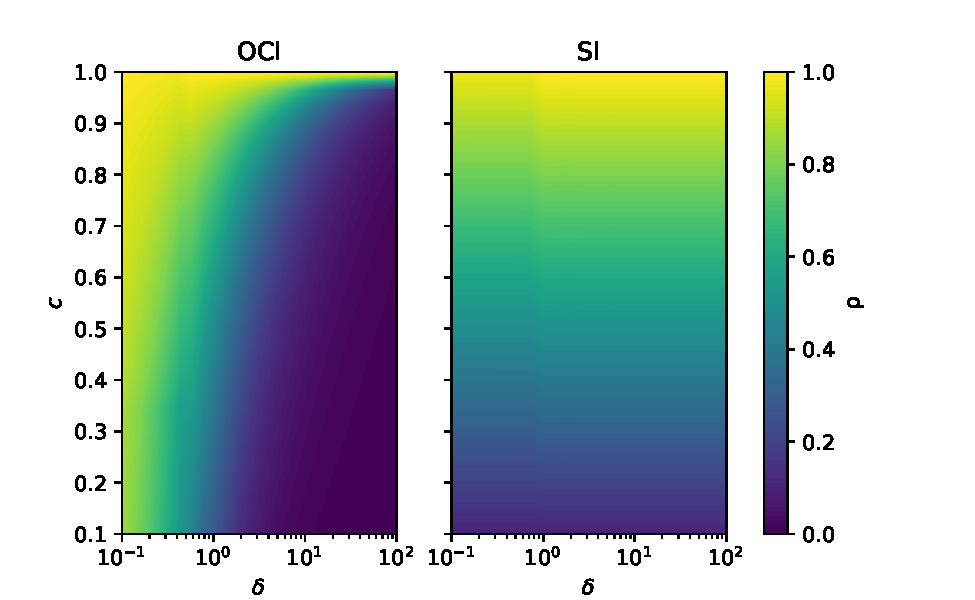
\includegraphics[width=\textwidth]{figures/therefore_figs/ss_specrads.pdf}
    \caption{Spectral radii (${\rho}$) of steady-state OCI (left) and SI (right), where $c$ is the scattering ratio and ${\delta}$ is the cellular optical thickness in mean free paths from Fourier analysis in S$_8$.}
    \label{fig:c2_ss-sepcrad}
\end{figure}

Others have explored OCI as an acceleration scheme for SI \cite{hoagland_hybrid_2021}, a component of a multi-grid solver \cite{man1995multigrid1, man1996multigrid2}, and a solution to the integral transport matrix method \cite{raffi2108pidotscom}.
However, previous investigations of OCI are limited to steady-state computations.

When employing implicit time-differencing schemes (e.g., Crank--Nicholson, backward Euler), each time step involves the solution of a steady-state transport problem with an effective total cross section that includes a time absorption term, proportional to $1/(v \Delta t)$, where $\Delta t$ is time step size and $v$ is radiation speed.
Returning to Fig.~\ref{fig:ss-sepcrad}, the macroscopic total cross section ($\Sigma$) influences both the optical thickness of the cell ($\delta$) and the scattering ratio ($c$), so increasing or decreasing $\Sigma$ will impact convergence behavior.
Spectral radius for both iterative methods decreases as the scattering ratio decreases, but \textit{the spectral radius of OCI also decreases with increasing optical thickness}, which in turn depends on $\Sigma$.
When solving optically thin and highly scattering problems, small increases to $\Sigma$ (and for time-dependent problems, decreases in $\Delta t$ or $v$) may drastically improve the relative performance of OCI compared to SI.
This hypothesis motivates our work, along with evaluating cell-wise algorithms on modern GPU accelerators and exploring higher-order space-time discretization schemes.

\subsection{Preconditioners and Synthetic acceleration}
\label{c2:precon}
Preconditioners can be used to aid convergence of iterative schemes for the neutron transport equation \cite{adams_fast_2002}.
Often physics informed preconditioners for transport iterations may be thought of as high-order method solving the full discretized transport equation and a low-order method informing intra-iteration updates to then be used in the next iteration of the high-order problem.
The low-order method is usually some physics-informed problem that is computationally cheaper to solve then the transport problem and models physical behavior that is difficult for a given operator splitting to converge (e.g., the diffusive limit, $c\rightarrow1$).

Synthetic acceleration schemes are a common subset of preconditioners for the source iteration operator splitting.
A synthetic acceleration method only \textit{accelerates} convergence to the same solution as transport and is fully consistent with the high-order transport method.
Generally for synthetic acceleration methods the low-order simulation is \textit{driven} by the error between iterates of a transport solve.
Synthetic acceleration techniques for source iterations include:
boundary projection acceleration \cite{adams_boundary_1988}, 
transport synthetic acceleration \cite{ramone_1997_tsa},
multi-grid methods \cite{man1994parallel},
and the venerable diffusion synthetic acceleration (DSA) \cite{larsen_1983_dsaforsn} among others.

Diffusion synthetic acceleration is a common preconditioner for the source iteration operator splitting \cite{adams_fast_2002, alcouffe_1977_dd, coale_2025_dsa}.
It implements a low-order diffusion solve driven by the error between subsequent transport iterations to inform a correction term for the scalar flux, which can in turn be used as the source in a subsequent high-order source iteration.
To make DSA consistent the specific structures of the low-order diffusion solve is governed by the spatial discretization scheme used in the high-order transport simulation.
Larsen's 4-step method can be used to yield a DSA scheme that is consistent with spatial discritization, however, the system of equations produced from a Larsen 4-step process can be difficult to solve, or forum inconsistent schemes for finite elements in higher dimensions \cite{larsen_1982_unconDSA, larsen_1982_unconDSAte, haut_2020_dsa}. 
The Adams-Martin modified 4-step process produces consistent schemes with finite element discritization methods \cite{adams_1992_dsadfe}.
Consistent DSA-SI schemes produce rapidly convergent iteration methods where $\rho<c/3$ in homogeneous regions.

Another class of physics informed preconditioners for the radiation transport equation that do not fall into the sub-category of synthetic acceleration are the moment expatiation methods including: second moment (also called Lewis \& Miller methods) \cite{olivier_2024_smoms, lewis_computational_1984, oliver_2025_secondmoment}, quasi-diffusion \cite{ani_1986_quasidiffusion, goldin_1964_quasidissuion}, and variable Eddington factor \cite{lou_2021_vef, coale_2024_rmomvef} methods.
All of these preconditioners are themselves a set of High-Low (HOLO) methods \cite{chacon_2017_holosurvey}.
They still use the same general algorithm as synthetic acceleration where information from the high-order transport solve somehow drives the low-order problem, often with additional physical characteristics (e.g., volumetric material source).
Then the low-order solution some how updates information going into the high-order system.
These methods are often inconsistent with the transport equation thus potentially solving a different physical interpretation of the problem physics, but they can be very rapidly convergent.

There is less research on preconditioners for OCI when used alone as the primary space-parallel iterative scheme.
OCI itself has previously been used as an acceleration method for source iterations in the forum of either a multi-grid in space solver \cite{kang2000oci, man1994parallel} or a true hybrid scheme (using the same transport mesh) with SI \cite{hoagland_hybrid_2021}.
Rosa and Warsa showed that transport synthetic acceleration (TSA) can resynchronize cells but TSA still requires a potentially expensive sweep operation \cite{tsa2009rosa}.
Figure \ref{fig:ss_spec_rads} at right shows the spectral radius of TSA-OCI (using no scattering information ($\beta=1$, e.g., a transport sweep between OCI solves).
Notably for OCI-TSA with $\beta=1$ the method is still potentially unconvergent in the diffusive limit.
However as $\beta\rightarrow0$ and more scattering physics is included in the low order simulation convergence in the diffusive limit will also be supported.
The search for non-sweeping---ideally space-parallel or otherwise computationally cheap---preconditioner for OCI to more rapidly converge in the diffusive and thin limits motivates this work.

Yavuz and Larsen described a second moment method they used to accelerate domain decomposed SI sweeps \cite{yavuz_spatial_1989}.
They use source iterations within a subdomain and Jacobi iterations to converge incident angular flux between subdomains.
Their method uses a low-order second moment system of equations to inform updates of incident angular flux on the boundaries of each subdomain.
Thus the high-order solver is \textit{not} the SI transport solve but instead the Jacobi iteration.
With their method Yavuz and Larsen showed decreased Jacobi iteration counts for 1D and 2D problems on rectilinear grids \cite{yavuz_spatial_1989, yavuz_1992_2ddd}.
This scheme may aid the convergence of OCI.


\section{Considerations for Parallel Computing}
\label{c2:hpc}


\section{Summary of Part and Relation to Research Questions}

Chapter \ref{chap:therefore_paper} analyzes how the convergence rate of an OCI scheme behaves when used for time-dependent neutron transport computations.
I derive a second-order space-time discretization method from the simple corner balance and multiple balance time discretization schemes and show via Fourier analysis that it is unconditionally stable through time.
Then, I derive and numerically solve the Fourier systems for both OCI and SI splittings of the discretization, showing that small mean-free times improve the spectral radius of OCI more than SI, and that the spectral radius for OCI tends to zero as mean free time gets smaller.
I extend both solvers to be energy dependent (using the multi-group assumption) and implement them on an AMD MI250X using vendor-supplied batched LAPACK solvers.
I show that smaller time steps improve the relative performance of OCI over SI, and, even when OCI requires more iterations to converge a problem, those iterations can be done much faster on a GPU.
This leads to OCI performing better overall than SI on GPUs.
This chapter answers research questions:
\begin{itemize}
    \item \emph{RQ1}: How to use software engineering libraries to implement work more efficiently;
    \item \emph{RQ2}: A space-parallel iterative scheme on modern HPC GPUs; and
    \item \emph{RQ3}: How transient behavior impacts convergence of a space-parallel iterative scheme.
\end{itemize}
This work is novel as it is the first time OCI has been implemented on modern GPUs, the firs time OCI has been used to solve transient systems, the first time the time dependent multiple balance approach has been used in conjunction with OCI or the simple corner balance spital discritization scheme, and the first published use of strided batched solvers for OCI on the GPU allowing the use of vendor supplied libraries instead of manually scripted GPU kernels.

Chapter \ref{chap:smom_paper} derives a preconditioner to converge OCI faster in the diffusive limit.
I derive a second moment cellular decomposition method in conjunction with a one-cell inversion iteration in an effort to produce a fully space parallel, rapidly convergent, transport iteration.
THe method we use is based on a preconditioner derived for domain decomposed problems.
The second moment preconditioner derived in this work does not converge to the same solution as unpreconditioned transport solutions suggesting inconsistencies between the high and low order equations.
Numerical experiments show the second moment preconditioner is rapidly convergent in the diffusive limit but dose not aid convergence in the optically thin limit.
This chapter answers research questions:
\begin{itemize}
    \item \emph{RQ1}: How to use software engineering libraries to implement work more efficiently on modern computing architectures; and
    \item \emph{RQ4}: How to accelerate the space-parallel iterative scheme to converge faster.
\end{itemize}


%Work in this part of my dissertation is in four independent variables in a single angle and spatial dimension.
%While this limits the practical applicability of the exact problems I am solving in this work, the methods may be imp
%In this work I limit to a single spatial dimension.
%This because the problems we are tying to solve (balancing parallelism, time dependence, convergence rate, and searching preconditioners) is dreadfully difficult.
%While the problems I solve are not
%In radiation transport it is common to develop novel numerical methods for simple slab wall problems as the linkage between must be correct in a single \cite{ragusa_robust_2012, larsen_asymptotic_1987, yauz, }
%Without good preconditioning the method described herein has extremely limited applicability to problems of interest which often contain optically thin cells.
%Wil
\newpage
\renewcommand{\TheTitle}{One-Cell Inversion for Solving Higher-Order Time-Dependent Radiation Transport on GPUs}
\renewcommand{\TheAuthors}{Joanna Piper Morgan,
  Ilham Variansyah,
  Todd S. Palmer, and
  Kyle E. Niemeyer}

\renewcommand{\TheAddress}{
    \textit{Acepted to Nuclear Science and Engineering} \\
    Vol.~VOLUME, PAGES, YEAR. \\
    \doi{10.1016/xxxx}
}

\PaperHeader{\TheTitle}{\TheAuthors}{\TheAddress}

\chapter{\TheTitle}
\label{chap:therefore_paper}

\epigraphhead[10]{\singlespacing
\epigraph{
    We loiter in the winter 
    while it is already spring.
	}{Henry David Thoreau}
}



\section*{Abstract}
To find deterministic solutions to the transient discrete-ordinates neutron-transport equation, source iterations (SI) are typically used to lag the scattering (and fission) source terms from subsequent iterations.
For Cartesian geometries in one dimension, SI is parallel over the number of angles but not spatial cells; this is a disadvantage for many-core compute architectures like graphics processing units.
One-cell inversion (OCI) is a class of alternative iterative methods that allow space-parallel radiation transport on heterogeneous compute architectures.
For OCI, previous studies have shown that, in steady-state computations, spectral radius tends to unity when cells are optically thin regardless of the scattering ratio.
In this work, we analyze how the convergence rate of an OCI scheme behaves when used for time-dependent neutron transport computations.
We derive a second-order space-time discretization method from the simple corner balance and multiple balance time discretization schemes and show via Fourier analysis that it is unconditionally stable through time.
Then, we derive and numerically solve the Fourier systems for both OCI and SI splittings of our discretization, showing that small mean-free times improve the spectral radius of OCI more than SI, and that spectral radius for OCI tends to zero as mean free time gets smaller.
We extend both solvers to be energy dependent (using the multi-group assumption) and implement on an AMD MI250X using vendor-supplied batched LAPACK solvers.
Smaller time steps improve the relative performance of OCI over SI, and, even when OCI requires more iterations to converge a problem, those iterations can be done much faster on a GPU.
This leads to OCI performing better overall than SI on GPUs.

\section{Introduction}

% more general intro problem applications -> Sn transport
Simulating transient particle transport is often required when computing the solution to a number of multi-physics problems, including burst criticality experiments, fission reactor accidents, and other highly dynamic systems.
% Problems to solve and Sn transport
Finding deterministic solutions to the transient neutron transport equation requires some method of treating the contribution of scattering described by an integral.
This is either done by taking moments of the neutron transport equation and making a closure assumption, or by using quadrature to discretize the integral over angle.
The latter is called the method of discrete ordinates (or S$_N$ method, where $N$ is the number of angles in a one-dimensional quadrature set) that forms a coupled set of simultaneous PDEs, with one for every direction in a given quadrature set.
The contribution to the scattering source can then be computed using a sum over angles of weights times quantities of interest.
Typically, iterative schemes from operator splitting are used to treat the scattering (and fission) source terms that arise in this coupled set of partial differential equations \cite{lewis_computational_1984}.

% State of the art of transport solvers on CPUs and GPUs warsaw paper
Source iteration (SI), often accompanied by preconditioners or synthetic accelerators, is a common iteration approach: the contribution to the solution from the scattering source lags, while the angular flux is solved in every ordinate direction via ``sweeps'' through the spatial domain~\cite{adams_subcell_1997}.
SI sweeps in Cartesian geometries readily parallelize over the number of angles.
While any parallelization improves performance, a scheme that is embarrassingly parallel over the dimension with the greatest number of degrees of freedom---space---would be advantageous, especially on vectorized hardware \cite{rosa_cellwise_2013, hoagland_hybrid_2021}.
In slab geometry, SI sweeps can be parallelized in angle and energy groups (via Jacobi iteration), but are serial in space as information about the angular flux incident on edges of each cell is required before the computation can proceed.

In higher spatial dimensions, many S$_N$ production codes that implement SI use a wavefront marching parallel algorithm known as a Koch--Baker--Alcouffe scheme \cite{baker_kba_2017}, also called ``full parallel sweeps.''
This algorithm begins a sweep in a spatial location where all cell dependencies are known from boundary information (e.g., a corner).
From there, on a hypothetical orthogonal 2D spatial grid the two nearest neighbor cells are computed independently in parallel; the next step would be across four cells.
This diagonally expanding wavefront continues to march and can compute quantities of interest in parallel for as many cells that lie on the diagonal sweep step.
These sweeps are done on structured or unstructured finite element or finite volume spatial discretizations with backward Euler or Crank--Nicholson time stepping iterations.
Source iteration is often solved with preconditioned fixed-point (Richardson) or Krylov sub-space methods (e.g., GMRES) \cite{adams_fast_2002}.

An alternative to SI is one-cell inversion (OCI), a class of operator splitting that computes all angular fluxes in all ordinates within a cell in a single linear algebra solve, assuming that the angular fluxes incident on the surfaces of the cell are known from a previous iteration \cite{kang2000oci}.
OCI methods allow parallelizing over the number of cells, as each cell is solved independently in parallel.
OCI iterations can take the form of a cell-wise block-Jacobi, cell-wise block-Gauss--Seidel, or cell-wise red-black iteration depending on the order in which cells are inverted \cite{man1994parallel}.
Like SI, OCI iterations can be fixed-point (Richardson) or non-stationary schemes like GMRES \cite{kylov2004warsa}, with or without preconditioners (including diffusion synthetic acceleration \cite{kang2000oci}) on structured and unstructured meshes.
Parallel block Jacobi and parallel block Gauss--Seidel iterations may also be used for domain decomposition with transport sweeps within subdomains \cite{qiao_improved_2021}.
In fact, OCI methods can be thought of as a cellular decomposed version of these schemes.

\cite{rosa_cellwise_2013} previously studied cell-wise block Jacobi and cell-wise block Gauss--Seidel as a potentially superior iterative scheme over SI preconditioned with diffusion synthetic acceleration on vectorized architectures.
They hypothesized that OCI schemes might outperform an SI preconditioned with diffusion synthetic acceleration and using full-parallel sweeps in terms of wall-clock runtime, because of OCI's parallelism over the dominant domain (space), the ability to take advantage of vendor-supplied LAPACK type libraries, high arithmetic-intensity operations present in an OCI algorithm, and superior spectral properties in the thick limit.
Rosa et al.\ conducted Fourier analysis for and implemented OCI in a 2D, multi-group, steady-state code using bilinear discontinuous finite elements to discretize space.
They paired this with either a cell-wise block Jacobi and cell-wise block Gauss--Seidel iteration algorithm.
The study was conducted on the (then) state-of-the-art RoadRunner supercomputer and took advantage of its 64-bit PowerXCell vectorized accelerator.
However, the acceleration per iteration in the block Gauss--Seidel OCI implementation did not make up for the degradation of convergence that OCI methods incur in the thin limit.

OCI can require more iterations to converge to a solution for some problems, since no information exchanges between cells within an iteration.
Specifically, as cellular optical thickness decreases, OCI's relative performance degrades.
Spectral radius ($\rho$) of OCI tends to unity in the thin cell limit---regardless of the scattering ratio---due to the algorithm decoupling cells from one another (i.e., asynchronicity) \cite{rosa_cellwise_2013, hoagland_hybrid_2021, man1994parallel}. 
Figure~\ref{fig:ss-sepcrad} illustrates this behavior, showing the spectral radii of the two iteration schemes as a function of cellular optical thickness, $\delta$ (in mean free paths), and the scattering ratio, $c$.
We compute these values using Fourier analysis of an infinite medium slab problem using S$_{8}$ angular quadrature for block Jacobi OCI and unpreconditioned SI iterative schemes\footnote{Gauss--Legendre quadrature is used in all presented work.}.
The spectral radius of SI depends strongly on the scattering ratio but is independent of $\delta$ for the homogeneous infinite-medium problem. 
Compared to SI, OCI rapidly converges in thicker cells, even in highly scattering problems except for scattering ratios closest to one.

\begin{figure}
    \centering
    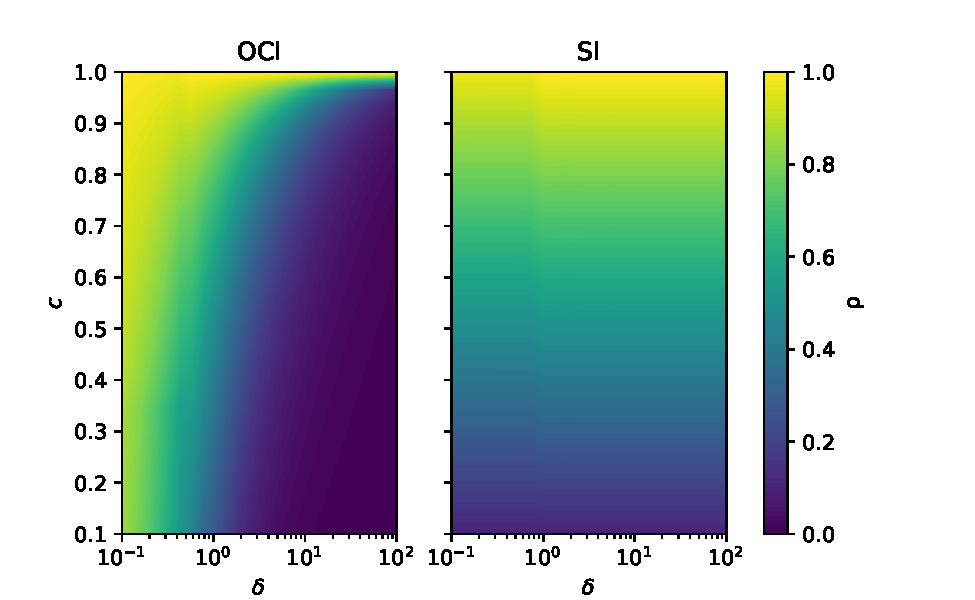
\includegraphics[width=\textwidth]{figures/therefore_figs/ss_specrads.pdf}
    \caption{Spectral radii (${\rho}$) of steady-state OCI (left) and SI (right), where $c$ is the scattering ratio and ${\delta}$ is the cellular optical thickness in mean free paths from Fourier analysis in S$_8$.}
    \label{fig:ss-sepcrad}
\end{figure}

Others have explored OCI as an acceleration scheme for SI \cite{ hoagland_hybrid_2021}, a component of a multi-grid solver \cite{man1995multigrid1, man1996multigrid2}, and a solution to the integral transport matrix method \cite{raffi2108pidotscom}.
However, previous investigations of OCI are limited to steady-state computations.

When employing implicit time-differencing schemes (e.g., Crank--Nicholson, backward Euler), each time step involves the solution of a steady-state transport problem with an effective total cross section that includes a time absorption term, proportional to $1/(v \Delta t)$, where $\Delta t$ is time step size and $v$ is radiation speed.
Returning to Fig.~\ref{fig:ss-sepcrad}, the macroscopic total cross section ($\Sigma$) influences both the optical thickness of the cell ($\delta$) and the scattering ratio ($c$), so increasing or decreasing $\Sigma$ will impact convergence behavior.
Spectral radius for both iterative methods decreases as the scattering ratio decreases, but \textit{the spectral radius of OCI also decreases with increasing optical thickness}, which in turn depends on $\Sigma$.
When solving optically thin and highly scattering problems, small increases to $\Sigma$ (and for time-dependent problems, decreases in $\Delta t$ or $v$) may drastically improve the relative performance of OCI compared to SI.
This hypothesis motivates our work, along with evaluating cell-wise algorithms on modern GPU accelerators and exploring higher-order space-time discretization schemes.

We previously derived a second-order space (simple corner balance), and time discretization (multiple balance) scheme for block Jacobi OCI (which we will call simply OCI in the remainder of this work) \cite{morgan2023oci}.
We previously showed that when there are more spatial degrees of freedom than in angle, a GPU implementation of OCI will outperform a similarly implemented version of SI in wall clock runtime, in all but the highest scattering problems, for quadrature orders between \num{16} and \num{64} for mono-energetic 1D problems. 

Some derivations from our previous work are included here (Section~\ref{sec:methods-derv}), because we extend it with a Fourier analysis of the discretization scheme through time to ensure it remains unconditionally stable.
We also perform a Fourier analysis on a single time step of OCI and SI to study convergence behaviors in various limits under transient conditions.
Furthermore we extend our derivations to multi-group problems and implement both OCI and SI on an AMD MI250X GPU using vendor-supplied libraries to confirm Fourier results and analyze performance.

\section{Methods}

In this section, we derive the discretized equations for the initial and boundary value problem and describe the OCI iteration.
We have chosen to implement robust second-order discretization methods: simple corner balance  \cite{adams_subcell_1997} in space and multiple balance \cite{variansyah_robust_2021} in time.
By coupling these higher accuracy schemes with an efficient iterative method, we hope to optimize the ratio of compute work to communication work to better suit the numerical method for GPUs.
To confirm that multiple balance time discretization remains unconditionally stable with simple corner balance, we conduct Fourier analysis for a non-scattering model problem.
Then, we derive the Fourier system for a single time step of simple corner balance + multiple balance discretization using both OCI and SI operator splitting to study the convergence rate.
Finally, we present systems for multi-group transport.

\subsection{Derivation of space and time discretization for one-cell inversion}
\label{sec:methods-derv}
We begin with the time-dependent, isotropic scattering slab geometry, S$_N$ transport equations with an isotropic source.
\begin{multline}
    \label{eq:sn_nte}
    \frac{1}{v} \frac{\partial \psi_{m}(x,t)}{\partial t} + \mu_m \frac{\partial \psi_{m}(x,t)}{\partial x} + \Sigma(x) \psi_{m}(x,t) 
     = \frac{1}{2} \left( \Sigma_{s}(x) \sum\limits_{n=1}^N w_n \psi_{n}(x,t) + Q(x,t) \right) \;, \\
    \qquad \qquad m=1, \ldots, N \;, \qquad t > 0 \;, \qquad x \in [0,X]
\end{multline} 
where $\psi$ is the angular flux, $t$ is time, $x$ is location, $v$ is speed, $\Sigma$ is the macroscopic total cross-section, $\Sigma_s$ is the macroscopic scattering cross-section, $w_m$ is angular quadrature weight, $\mu_m$ is the angular quadrature ordinate, $m$ is the quadrature index, $N$ is the quadrature order, and $Q$ is the isotropic material source.
The initial and boundary conditions are prescribed angular flux distributions:
\begin{equation*}
    \psi_{m}(x,0) = \psi_{init,m}(x), \qquad m=1 \ldots N \;,
\end{equation*}
\begin{equation*}
    \psi_{m}(0,t) = \psi_{inc,m}^+(t), \qquad \mu_m >0 \;,
\end{equation*}
\begin{equation*}
    \psi_{m}(X,t) = \psi_{inc,m}^-(t), \qquad \mu_m <0 \;.
\end{equation*}
We discretize these equations in time using multiple balance~\cite{variansyah_robust_2021}, which solves two coupled sets of equations. 
First is a backward Euler step (transport equation integrated over a time step):
\begin{subequations}
\begin{multline}
\frac{1}{v} \left( \frac{\psi_{m,k+1/2}(x) - \psi_{m,k-1/2}(x)}{\Delta t} \right) + \mu_m \frac{\partial \psi_{m,k}(x)}{\partial x} + \Sigma(x) \psi_{m,k}(x) \\
= \frac{1}{2} \left(  \Sigma_{s}(x) \sum\limits_{n=1}^N w_n \psi_{n,k}(x) + Q_{k}(x) \right) \;,
\end{multline}
and the second is a balance like auxiliary equation from the multiple balance principle:
\begin{multline}
\frac{1}{v} \frac{\psi_{m,k+1/2}(x) - \psi_{m,k}(x)}{\Delta t/2} + \mu_m \frac{\partial \psi_{m,k+1/2}(x)}{\partial x} + \Sigma(x) \psi_{m,k+1/2}(x) \\
= \frac{1}{2} \left( \Sigma_{s}(x) \sum\limits_{n=1}^N w_n \psi_{n,k+1/2}(x) + Q_{ k+1/2}(x) \right) \;,
\end{multline}
\end{subequations}
where $\Delta t$ is the time step size, $k$ indicates time-average quantities, and $k\pm1/2$ indicates time-edge quantities.
Then, we discretize in space using simple corner balance, which involves a spatial integration over the right and left halves of a spatial cell:
\begin{subequations}
\label{eq:scb-mb}
\begin{multline}
\label{eq:scb-mb-a}
\frac{\Delta x_j}{2} \frac{1}{v} \left( \frac{\psi_{m,k+1/2,j,L} - \psi_{m,k-1/2,j,L}}{\Delta t} \right)
 + \mu_m \left[ \frac{\left( \psi_{m,k,j,L} + \psi_{m,k,j,R} \right)}{2}  - \psi_{m,k,j-1/2} \right] \\
+ \frac{\Delta x_j}{2} \Sigma_{j} \psi_{m,k,j,L} 
= \frac{\Delta x_j}{2} \frac{1}{2} \left( \Sigma_{s,j} \sum\limits_{n=1}^N w_n \psi_{n,k,j,L} + Q_{k,j,L} \right) \;,
\end{multline}  
\begin{multline}
\label{eq:scb-mb-b}
\frac{\Delta x_j}{2} \frac{1}{v} \left( \frac{\psi_{m,k+1/2,j,R} - \psi_{m,k-1/2,j,R}}{\Delta t} \right) +
\mu_m \left[ \psi_{m,k,j+1/2} - \frac{\left( \psi_{m,k,j,L} + \psi_{m,k,j,R} \right)}{2}   \right] \\
+ \frac{\Delta x_j}{2} \Sigma_{j} \psi_{m,k,j,R} = \frac{\Delta x_j}{2} \frac{1}{2} \left( \Sigma_{s,j} \sum\limits_{n=1}^N w_n \psi_{n,k,j,R} + Q_{k,j,R} \right) \;,
\end{multline}  
\begin{multline}
\label{eq:scb-mb-c}
\frac{\Delta x_j}{2} \frac{1}{v} \left( \frac{\psi_{m,k+1/2,j,L} - \psi_{m,k,j,L}}{\Delta t/2} \right) \\
+ \mu_m \left[ \frac{\left( \psi_{m,k+1/2,j,L} + \psi_{m,k+1/2,j,R} \right)}{2}  - \psi_{m,k+1/2,j-1/2} \right]
+ \frac{\Delta x_j}{2} \Sigma_{j} \psi_{m,k+1/2,j,L} \\
= \frac{\Delta x_j}{2} \frac{1}{2} \left( \Sigma_{s,j} \sum\limits_{n=1}^N w_n \psi_{n,k+1/2,j,L} + Q_{k+1/2,j,L} \right) \;,
\end{multline}    
\begin{multline}
\label{eq:scb-mb-d}
\frac{\Delta x_j}{2} \frac{1}{v} \left( \frac{\psi_{m,k+1/2,j,R} - \psi_{m,k,j,R}}{\Delta t/2} \right) + \\
\mu_m \left[ \psi_{m,k+1/2,j+1/2} - \frac{\left( \psi_{m,k+1/2,j,L} + \psi_{m,k+1/2,j,R} \right)}{2}   \right]
+ \frac{\Delta x_j}{2} \Sigma_{j} \psi_{m,k+1/2,j,R} \\
= \frac{\Delta x_j}{2} \frac{1}{2} \left( \Sigma_{s,j} \sum\limits_{n=1}^N w_n \psi_{n,k+1/2,j,R} + Q_{k+1/2,j,R} \right) \;,
\end{multline} 
\end{subequations}
where $\Delta x$ is the cell width, $j$ is the spatial cell index, $L/R$ is the left or right half cell, respectively.
These equations contain the first of the two simple spatial closures---the angular flux at the cell midpoint is a simple average of the two half-cell average quantities:
\begin{subequations}
\begin{equation}
  \psi_{m,k}(x_j) =  \frac{\left( \psi_{m,k,j,L} + \psi_{m,k,j,R} \right)}{2} \;,
\end{equation}
\begin{equation}
  \psi_{m,k+1/2}(x_j) =  \frac{\left( \psi_{m,k+1/2,j,L} + \psi_{m,k+1/2,j,R} \right)}{2} \;.
\end{equation}
\end{subequations}
The second closure is an \textit{upstream} prescription for the cell-edge angular flux:
\begin{subequations}
    \begin{equation}
      \psi_{m,k,j+1/2} =
      \begin{cases}
      \psi_{m,k,j,R}, & \mu_m > 0, \\
      \psi_{m,k,j+1,L}, & \mu_m < 0 \;,
      \end{cases}
    \end{equation}
    \begin{equation}
      \psi_{m,k+1/2,j+1/2} =
      \begin{cases}
      \psi_{m,k+1/2,j,R}, & \mu_m > 0, \\
      \psi_{m,k+1/2,j+1,L}, & \mu_m < 0 \;.
      \end{cases}
    \end{equation}
\end{subequations}

Figure~\ref{fig:stencil} shows the stencil location for angular flux and source terms.
Figure~\ref{fig:stencil} shows the stencil location for angular flux and source terms. 
\begin{figure}
    \centering
    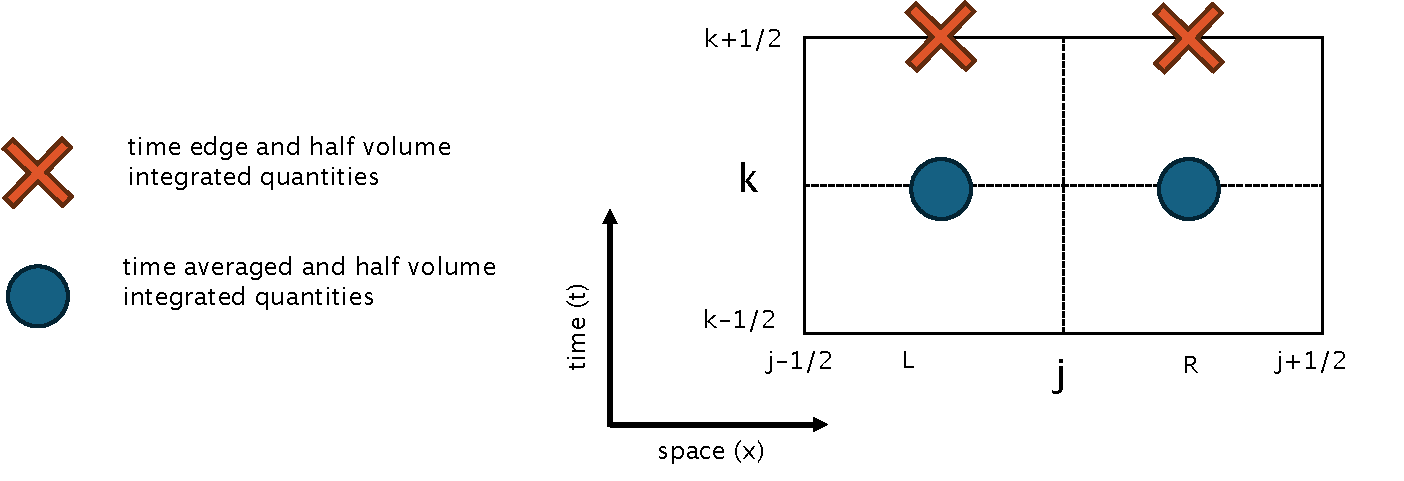
\includegraphics[width=\textwidth]{figures/therefore_figs/stencil.pdf}
    \caption{Discretization stencil for simple corner balance, multiple balance time discretization}
    \label{fig:stencil}
\end{figure}

Solving Eqs.~\eqref{eq:scb-mb} iteratively requires operator splitting.
Unknown values (from the current iteration, noted by $(l+1)$) are moved to the left-hand side to form a large system of linear equations.
In SI, the scalar flux in the scattering source is evaluated at the previous iteration $(l)$, decoupling angles and coupling space.
OCI allows the fluxes incident to the cell---defined by upstream closures---to lag, thus decoupling cells from one another within an iteration.

In OCI, the scattering source is subtracted to the left-hand side and  prior iteration values are employed for all information incident on cell $j$ (moved to the right-hand side).
This means that all $4N$ angular fluxes ($N$ angles at $L$ and $R$, $k$ and $k+1/2$) are computed simultaneously in cell $j$.
This yields a linear system for each cell $j$:
\begin{equation}
    \label{eq:oci}
    \left( \bm{L}_{c,j} - \bm{S}_j \right) \Psi_j^{(l+1)} = -\textbf{L}_{b,j} \Psi_j^{(l)} + \textbf{Q} \;, 
\end{equation}
where $l$ is the iteration index.
The right-hand side can be combined into a known vector
\begin{equation}
     \left( \bm{L}_{c,j} - \bm{S}_j \right) \Psi_j^{(l+1)}  = \bm{b}_j \; ,
\end{equation}
where $\bm{L}_{c,j}$ and $\bm{S}_j$ are both of size $4N\times4N$ and likewise $\bm{b}_j$ is a vector of length $4N$.
\newcommand{\lcmj}[1]{\begin{bmatrix} \bm{L}_{c,j,#1} \end{bmatrix} }
\newcommand{\zeros}{\begin{bmatrix} 0 \end{bmatrix} }
The within-cell operator is
\begin{subequations}
\begin{equation}
    \label{eq:Aja}
    \bm{L}_{c,j} = \begin{bmatrix}
        \lcmj{1} &  &  &  &  \\
          & \ddots  &  &  & \\
          &  & \lcmj{m} &  & \\
          &  &  & \ddots &  \\
          &  &  &  & \lcmj{N}
    \end{bmatrix} \;,
\end{equation}
with zeros elsewhere, where
\begin{equation} \bm{L}_{c,j,m} =
    \label{eq:Aj}
    \begin{bmatrix}
    \frac{|\mu_m| + \Delta x_j \Sigma_{j} }{2}  & \frac{\mu_m}{2} & \frac{\Delta x_j}{2 v \Delta t} & 0 \\
    - \frac{\mu_m}{2} & \frac{|\mu_m| +  \Delta x_j \Sigma_{j,g} }{2} & 0 & \frac{\Delta x_j}{2 v \Delta t} \\
    -\frac{\Delta x_j}{v \Delta t}  & 0 & \frac{\Delta x_j}{v \Delta t} + \frac{|\mu_m| + \Delta x_j \Sigma_{j,g} }{2}  & \frac{\mu_m}{2}  \\
    0 &  -\frac{\Delta x_j}{v \Delta t}  &  - \frac{\mu_m}{2} & \frac{\Delta x_j}{v \Delta t}+ \frac{|\mu_m| + \Delta x_j \Sigma_{j,g}}{2}  \\
    \end{bmatrix} \; .
\end{equation}
\end{subequations}
The right-hand side is
\begin{subequations}
\label{eq:rhs_sg}
\begin{equation}
    \bm{b}_j =  \left[
    \bm{b}_{j,1} \; \bm{b}_{j,2} \; \cdots \; \bm{b}_{j,N} \right]^{T} \;.
\end{equation}
As the linear system in each cell contains contributions from all angles (both positive and negative) $b_{j,m}$ is given by
\begin{equation} 
    \bm{b}_{j,m} = 
    \begin{cases}
        \bm{b}_{j,m}^+ & \mu_m>0 \\
        \bm{b}_{j,m}^- & \mu_m<0 \\
    \end{cases} \;,
\end{equation}
where
\begin{equation}
     \bm{b}_{j,m}^+ = \begin{bmatrix}
     \frac{\Delta x_j}{4} Q_{k,j,L} + \frac{\Delta x_j}{2 v \Delta t} \psi_{m,k-1/2,j,L} + \mu_m \psi^{(l)}_{m,k,j-1,R} \\
     \frac{\Delta x_j}{4}Q_{k,j,R} + \frac{\Delta x_j}{2 v \Delta t} \psi_{m,k-1/2,j,R} \\
     \frac{\Delta x_j}{4}Q_{k+1/2,j,L} + \mu_m \psi^{(l)}_{m,k+1/2,j-1,R} \\
     \frac{\Delta x_j}{4} Q_{k+1/2,j,R} 
    \end{bmatrix} \;,
\end{equation}
and
\begin{equation}
    \bm{b}_{j,m}^- = \begin{bmatrix}
    \frac{\Delta x_j}{4}  Q_{k,j,L} + \frac{\Delta x_j}{2 v \Delta t} \psi_{m,k-1/2,j,L}  \\
    \frac{\Delta x_j}{4}  Q_{k,j,R} + \frac{\Delta x_j}{2 v \Delta t} \psi_{m,k-1/2,j,R} - \mu_m \psi^{(l)}_{m,k,j+1,L}  \\
    \frac{\Delta x_j}{4}  Q_{k+1/2,j,L}  \\
    \frac{\Delta x_j}{4}  Q_{k+1/2,j,R} - \mu_m \psi^{(l)}_{m,k+1/2,j+1,L}
    \end{bmatrix} \;.
\end{equation}
\end{subequations}
The elements of the ${S_j}$ matrix are defined by
\begin{equation}
    \label{eq:scatter}
   [\mathbf{S}_j]_{k,l} = \begin{cases}
			\frac{\Delta x_j \Sigma_{s,j}}{4}w_{\frac{|(r-s)|}{3}}, & \text{if $\mod{\frac{(r-s)}{3} =0}$}\\
            0, & \text{otherwise}
		 \end{cases} \; ,
%  \frac{\Delta x_j \Sigma_{s,j}}{4} w_n \; l=r k=s
\end{equation}
where $w$ are the angular quadrature weights, and $r$ and $s$ are the rows and columns of the scattering matrix, respectively.
Finally,
\begin{subequations}
\label{eq:x_vec}
\begin{equation}
\Psi^{(l+1)}_j =  \begin{bmatrix}
    \bm{\psi}_{j,1}^{(l+1)}, \;
    \bm{\psi}_{j,2}^{(l+1)}, \;
    \cdots \;
    \bm{\psi}_{j,N}^{(l+1)}
    \end{bmatrix} ^{T} \; ,
\end{equation}
where
\begin{equation} 
\bm{\psi}_{j,n}^{(l+1)} = \begin{bmatrix}
    \psi_{n,k,j,L}^{(l+1)}, \;
    \psi_{n,k,j,R}^{(l+1)}, \;
    \psi_{n,k+1/2,j,L}^{(l+1)}, \;
    \psi_{n,k+1/2,j,R}^{(l+1)}
    \end{bmatrix}^{T} \;.
\end{equation}
\end{subequations}
One-cell inversion iterations continue until
\begin{equation}
    ||\Psi^{(l+1)}-\Psi^{(l)}||_{2} < \epsilon(1-\rho_e) \; ,
\end{equation}
where $\epsilon$ is the convergence tolerance and
\begin{equation}
    \rho_e = \frac{||\Psi^{(l+1)}-\Psi^{(l)}||_{2}}{||\Psi^{(l)}-\Psi^{(l-1)}||_{2}} \; ,
\end{equation}
is an empirical estimation of the spectral radius computed at every iteration of a transport solve.
After convergence, the time-step counter increments and the time-step process can be repeated.

Generally, Jacobi and Gauss--Seidel iterations converge faster when a system is more diagonally dominant \cite{isaacson_numerical_1966, golub_matrix_1983}.
Equation~\eqref{eq:Aj} contains ($ \delta/2 = \Delta x\Sigma/2 $) on the diagonals.
So in the thin limit (when $\delta\rightarrow 0$) the system becomes overall less diagonally dominant and converges more slowly.
However Equation~\eqref{eq:Aj} also involves $\Delta x/(v\Delta t)$ terms in elements (3,3) and (4,4).
Thus, a smaller time step will cause the system to become more diagonally dominant.
We provide a similar description of simple corner balance and multiple balance time discretization for an unpreconditioned source iteration \cite{morgan2023oci}.

\subsection{Fourier analysis: time-stepping scheme}

To ensure that the combination of higher-order discretization schemes remains an unconditionally stable time-marching method, we perform Fourier analysis (also known as Von Neumann stability analysis)~\cite{leveque2007finite}.
A time marching scheme
\begin{equation}
    \Psi_{k+1/2} = \bm{K} \Psi_{k-1/2} \;,
\end{equation}
where $\bm{K}$ is the time iteration matrix, is unconditionally stable when the Von Neumann stability condition is met:
\begin{equation}
    \sup(|\lambda_{K}|) \leq 1 \;,
    \label{eq:unconstab}
\end{equation}
where $\lambda_{K}$ are all the eigenvalues of $\bm{K}$ \cite{golub_matrix_1983, isaacson_numerical_1966}.
$\bm{K}$ can be derived for a given model problem.
We consider a model problem consisting of a homogeneous infinite medium with no scattering to derive the eigenfunction of the time-dependent multiple balance, simple corner balance discretization scheme.
Since this problem has no scattering, each angle can be solved independently of every other angle, and no operator splitting is required.
We first start by describing the absolute error of the angular flux at time step $(k+1/2)$:
\begin{equation}
    \mathbf{f}_{k+1/2} = \Psi_{\text{exact}} - \Psi_{k+1/2} \;.
\end{equation}
We then assume that each unknown representing the error on our discretization stencil is expanded in a series of temporal Fourier modes, where each mode has a coefficient ($a$, $b$, $c$, or $d$), an amplitude ($\lambda$), and a shape function ($e^{i\omega x}$).
We can then define a Fourier ansatz for the error propagated through a time step:
\begin{subequations}
\begin{align}
    f_{k+1/2,j,L} &= \lambda^{k+1}a e^{i\omega j} \; ,
    &
    f_{k+1/2,j,R} &= \lambda^{k+1}b e^{i\omega j} \; ,
\end{align}
\begin{align}
    f_{k,j,L} &= \lambda^{k}c e^{i\omega j} \; ,
    &
    f_{k,j,R} &= \lambda^{k}d e^{i\omega j} \; ,
\end{align}
\begin{align}
    f_{k-1/2,j,L} &= \lambda^{k}a e^{i\omega j} \; ,
    &
    f_{k-1/2,j,R} &= \lambda^{k}b e^{i\omega j} \; ,
\end{align}
\end{subequations}
where $k$ is the time step, $i=\sqrt{-1}$, $\lambda$ is the eigenvalue, $\omega$ is the wave number, and $j$ is cell index. 
Substituting our ansatz into the error form of Eqs.~\eqref{eq:scb-mb} and assuming $\mu>0$, we simplify to form
\begin{subequations}
\begin{equation}
    \label{eq:eig1}
    \frac{\Delta x}{2} \frac{1}{v \Delta t} (\lambda a- a) + \mu \left(\frac{c+d}{2} - d e ^{-i\omega} \right) + \frac{\Sigma\Delta x }{2}c = 0 \; ,
\end{equation}
\begin{equation}
\label{eq:eig2}
    \frac{\Delta x}{2} \frac{1}{v \Delta t} (\lambda b - b) + \mu \left( ce^{i\omega} - \frac{c+d}{2} \right) + \frac{\Sigma\Delta x }{2}d = 0 \; ,
\end{equation}
\begin{equation}
\label{eq:eig3}
    \frac{\Delta x}{2} \frac{2}{v \Delta t} (\lambda a - c) + \lambda\mu \left( \frac{a+b}{2} - b e^{-i\omega} \right) + \frac{\Sigma\Delta x }{2}a \lambda = 0 \; ,
\end{equation}
\begin{equation}
\label{eq:eig4}
    \frac{\Delta x}{2} \frac{2}{v \Delta t} (\lambda b - d) + \lambda\mu \left( d e^{i\omega} + \frac{c+d}{2} \right) + \frac{\Sigma\Delta x}{2} b\lambda = 0 \;.
\end{equation}
\end{subequations}
Next, we combine Eq.~\eqref{eq:eig1} into \eqref{eq:eig2}:
\begin{equation}
    \label{eq:f_a-1}
    \begin{bmatrix}
        c\\d
    \end{bmatrix}
    = \bm{K_{+}}^{-1} \frac{\Delta x}{2}\frac{1}{v\Delta t}(1-\lambda)
    \begin{bmatrix}
        a\\b
    \end{bmatrix} \;,
\end{equation}
where
\begin{equation}
    {\bm{K_{+}}} = 
    \begin{bmatrix}
    \frac{\mu}{2}+\frac{\Sigma \Delta x}{2} & \mu (\frac{1}{2} - e^{-i\omega}) \\
    -\frac{\mu}{2} & \frac{\mu}{2}+\frac{\Sigma \Delta x}{2}
    \end{bmatrix} \;.
\end{equation}
Then, doing the same with Eq.~\eqref{eq:eig3} into \eqref{eq:eig4}:
\begin{equation}
    \label{eq:f_a-2}
    \lambda \left( \bm{K_{+}} + \frac{\Delta x}{v \Delta t} \bm{I} \right)  \begin{bmatrix}
        a \\ b
    \end{bmatrix} = \frac{\Delta x}{v\Delta t} \begin{bmatrix}
        c \\ d
\end{bmatrix} \; ,
\end{equation}
where $\bm{I}$ is the identity matrix. Combining Eq.~\eqref{eq:f_a-1} into \eqref{eq:f_a-2} gives
\begin{equation}
    \lambda
    \begin{bmatrix}
        a \\b
    \end{bmatrix}
    = \left[ \bm{K_{+}} + \frac{\Delta x}{v\Delta t} \bm{I} + \gamma\bm{K_{+}}^{-1} \right]^{-1} \gamma \bm{K_{+}}^{-1}
    \begin{bmatrix}
        a \\ b
    \end{bmatrix} \; ,
\end{equation}
where $\gamma = \frac{\Delta x}{v\Delta t}  \frac{\Delta x}{2v\Delta t}$.
This can then be more appropriately posed as an eigenfunction:
\begin{equation}
    \lambda_K
    \bm{a}
    = \bm{K} \bm{a}\;,
\end{equation}
where
\begin{equation}
    \bm{K} = \gamma \left( \bm{K_{+}}\bm{K_{+}} + \frac{\Delta x}{v \Delta t}\bm{K_{+}} + \gamma \bm{I}\right)^{-1}
\end{equation}
and the eigenvector is
\begin{equation}
    \bf{a} = \begin{bmatrix}
        a, & b
    \end{bmatrix} ^T \;.
\end{equation}
The analysis is similar for $\mu<0$ only with
\begin{equation}
    \bm{K_{-}} = \begin{bmatrix}
        -\frac{\mu}{2} + \frac{\Sigma\Delta x}{2} & \frac{\mu}{2} \\
        \mu \left ( e^{i\omega} - \frac{1}{2} \right) & -\frac{\mu}{2} + \frac{\Sigma\Delta x}{2} 
    \end{bmatrix} \;.
\end{equation}

This system can be numerically solved after making discrete selections of $\mu \in [-1, 1]$ and $\omega \in (0,2\pi]$ at a point in the perameter space ($\Delta x$, $\Delta t$, $v$, $\Sigma$) with \texttt{numpy.max(\\numpy.abs(numpy.linalg.eig(K)))}~\cite{harris2020array}.

Figure \ref{fig:mb-scb} shows the absolute value of the maximum eigenvalues of $\bm{K}$ at various points in mean free time ($\tau=\Sigma v\Delta t$) and cellular optical thickness ($\delta=\Sigma\Delta x$) at 75 discrete points $\omega \in (0,2\pi]$ in S$_{16}$.
None of $|\lambda_{max}|$ are above one, which means the Von Neumann stability criterion in Eq. \eqref{eq:unconstab} is satisfied and the combination of the multiple balance time discretization and the simple corner balance scheme is unconditionally stable for this infinite homogeneous medium problem with no scattering.

\begin{figure}
    \centering
    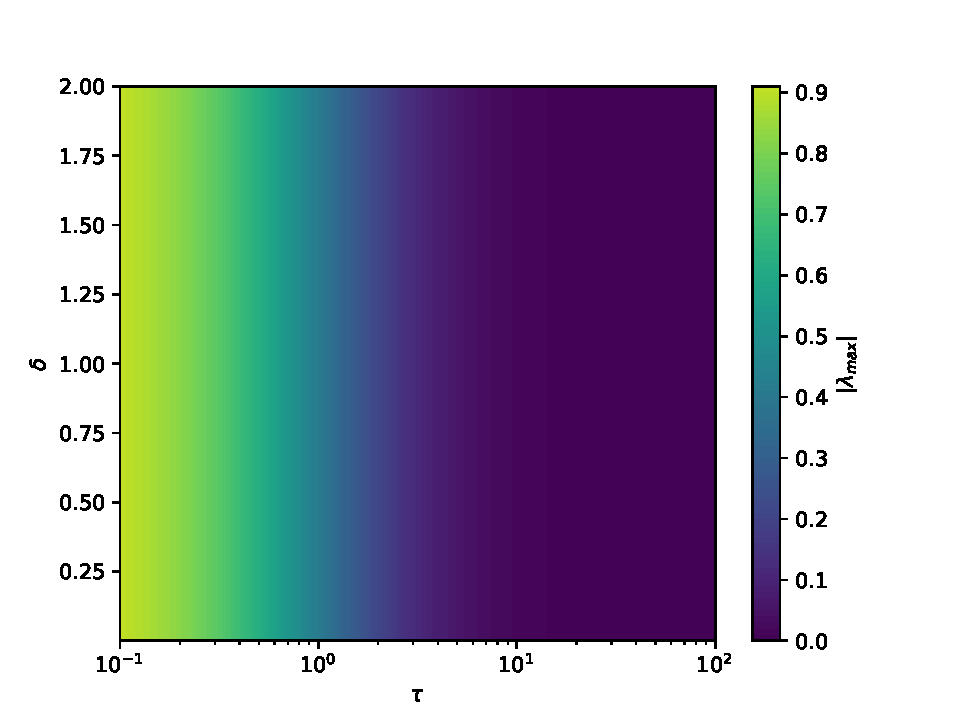
\includegraphics[width=0.9\linewidth]{figures/therefore_figs/mb_scb.pdf}
    \caption{$|\lambda_{\max}|$ from numerically solved multiple balance time discretization and simple corner balance Fourier system over choices in mean free time ($\tau$) and cellular optical thickness ($\delta$) in S$_{16}$.}
    \label{fig:mb-scb}
\end{figure}

\subsection{Fourier analysis: OCI iterative scheme}
\label{sec:methods-faoci}
\newcommand{\exi}{e^{i\lambda\Sigma x_j}}
\newcommand{\omlp}{\omega^{(l+1)}}
\newcommand{\oml}{\omega^{(l)}}
\newcommand{\dx}{\Delta x}
\newcommand{\dt}{\Delta t}
\newcommand{\scatsum}{\sum^{M}_{n=0}}

To study the impact of time dependence on the convergence of an OCI iteration, we conduct a Fourier analysis on the error equation of an infinite-homogeneous medium model problem in slab geometry in a single time step.
Similar to the analysis in the previous section, we can assert that for an iteration scheme
\begin{equation}
    \Psi^{(l+1)} = \bm{T} \Psi^{(l)} \;,
\end{equation}
where $(l)$ is the iteration counter, convergence rate is
\begin{equation}
   \rho = \sup(|\bm{\lambda}_{\bm{T}}|)\;,
\end{equation}
 where $\lambda_{\bm{T}}$ contains the eigenvalues of $\bm{T}$ \cite{golub_matrix_1983, isaacson_numerical_1966}.
An iterative method will converge if and only if $\rho<1$. 
Furthermore, iterations converge faster for smaller $\rho$.

To derive the transport matrix $\bm{T}$ we can again use Fourier separation analysis on a model problem.
We first start by describing the absolute error of the angular flux at iteration step $(l)$
\begin{equation}
    \mathbf{f}^l = \Psi^{\text{converged}} - \Psi^l \;,
\end{equation}
and our Fourier ansatz on a functional form of that error
\begin{subequations}
    \label{eq:anz}
    \begin{align}
        f^{(l)}_{m,k,j,L/R} &= \omega^{(l)}a_{m,L/R}e^{i\lambda\Sigma x_j} \; ,
        &
        f^{(l)}_{m,k+1/2,j,L/R} &= \omega^{(l)}b_{m,L/R}e^{i\lambda\Sigma x_j} \;.
    \end{align}
\end{subequations} 
The upstream closures at the left boundary of the cell are
\begin{subequations}
\begin{equation}
    f_{m,k,j-1/2} =
    \begin{cases}
        f_{m,k,j-1, R} \;, & \mu > 0 \\
        f_{m,k,j, L} \;, & \mu < 0 
    \end{cases} \;,
\end{equation}
and at the right are
\begin{equation}
    f_{m,k,j+1/2} =
    \begin{cases}
        f_{m,k,j, R} \;, & \mu > 0 \\
        f_{m,k,j+1, L} \;, & \mu < 0 
    \end{cases} \;.
\end{equation}
\end{subequations}

Now, substitute the ansatz and upstream closures into the error form of Eq. \eqref{eq:scb-mb} and derive the eigensystem.
This is done by (1) collecting like terms, (2) dividing both sides by $\omega^{(l)} e^{i\Sigma x_j}$, (3) isolating terms with a remaining $\omega$ to the left-hand side, and finally (4) forming the eigensystem into the iteration matrix over all angular directions:
\begin{equation}
    \bm{T}_{OCI} = \left( 
    \bm{L}_c
    - \bm{S}
    \right)^{-1}
    \begin{bmatrix}
        \bm{L}_b^- & 0\\
        0 & \bm{L}_b^+
    \end{bmatrix} \;,
\end{equation}
which now forms a well-posed eigenvalue problem over all angles:
\begin{equation}
    \lambda\bm{a} = \bm{T} \bm{a} \; ,
\end{equation}
where the eigenvector $\mathbf{a}$ is defined by
\begin{equation}
    \mathbf{a} = \begin{bmatrix}
        a_{1} & a_{2} & \cdots & a_M
    \end{bmatrix} ^T \;,
\end{equation}
\begin{equation}
    a_m = \begin{bmatrix}
        a_{mR} & a_{mL} & b_{mR} & b_{mL} 
    \end{bmatrix} ^T \; ,
\end{equation}
$\bm{L}_c$ is the linear within-cell transport operator defined by Eqs.~\eqref{eq:Aja} and \eqref{eq:Aj}, 
\begin{equation}
    \bm{L}_b^+ = 
    \begin{bmatrix}
        0 & 0 & 0 & 0 \\
        -\mu_m e^{-i\lambda\sigma\dx} & 0 & 0 & 0 \\
        0 & 0 & 0 & 0 \\
        0 & 0 & -\mu_m e^{-i\lambda\sigma\dx} & 0
    \end{bmatrix} \; ,
\end{equation}
and
\begin{equation}
    \bm{L}_b^- = 
    \begin{bmatrix}
        0 & \mu_m e^{i\lambda\sigma\dx} & 0 & 0 \\
        0 & 0 & 0 & 0 \\
        0 & 0 & 0 & \mu_m e^{i\lambda\sigma\dx} \\
        0 & 0 & 0 & 0
    \end{bmatrix} \; .
\end{equation}
The scattering matrix is again akin to the previously described transport matrix in Eq.~\eqref{eq:scatter}.
Finally, to numerically evaluate the spectral radius we form the system for a given set of angles and weights from Gauss--Legendre quadrature and solve with \texttt{numpy.max(numpy.abs(\\numpy.linalg.eig(T)))} for $\omega \in [0,2\pi]$ at discrete points.
We vary the cellular optical thickness ($\delta =\Sigma \Delta x$), mean free time ($\tau = \Sigma v\Delta t$), and scattering ratio ($c=\Sigma_s/\Sigma$) to study convergence behavior in various physical regimes. 
The analogous eigensystem for source iteration is
\begin{equation}
    \bm{T}_{SI} = \left( 
    \bm{L}_c
    + \begin{bmatrix}
        \bm{L}_b^- & 0\\
        0 & \bm{L}_b^+
    \end{bmatrix}
    \right)^{-1}
    \bm{S} \; .
\end{equation} 
Section~\ref{sec:results-faoci} contains the results of this analysis.


\subsection{OCI multi-group transport}

We extend our single-energy derivations presented in Section~\ref{sec:methods-derv} to be energy dependent. 
Elements of the $\mathbf{S_{g' \rightarrow g}}$ matrix are now defined by
\begin{equation}
    \label{eq:scatter_mg}
   [\mathbf{S}_{g' \rightarrow g,j}]_{k.l} = \begin{cases}
			\frac{\Delta x_j \Sigma_{s,g'\rightarrow g,j}}{4}w_{\frac{|(r-s)|}{3}}, & \text{if $\mod{\frac{(r-s)}{3} =0}$}\\
            0, & \text{otherwise}
		 \end{cases} \; ,
%  \frac{\Delta x_j \Sigma_{s,j}}{4} w_n \; l=r k=s
\end{equation}
where $g' \rightarrow g$ indicates transfer from group $g'$ to group $g$ and $w$ are the quadrature weights. 
\begin{subequations}
\label{eq:fullOCI_mg}
The full system of linear equations in all groups and angles in cell $j$ becomes
\begin{equation}
    \bm{A}_j \bm{\Psi}_j = \bm{b}_j \; ,
\end{equation}
where
\begin{equation}
    \label{eq:fullOCIlhs}
    \bm{A}_j = 
    \begin{bmatrix}
        \bm{L}_{c,j,1} -\bm{S}_{1\rightarrow1,j} & -\bm{S}_{2\rightarrow1,j} & \cdots & \cdots& -\bm{S}_{G\rightarrow1,j}\\
        -\bm{S}_{1\rightarrow2,j} & \ddots & & & \vdots\\
         \vdots & & \bm{L}_{c,j,g}-\bm{S}_{g\rightarrow g,j} &  & \vdots\\
        \vdots & &  &  \ddots & \vdots \\
        -\bm{S}_{1\rightarrow G,j} & \cdots & \cdots & & \bm{L}_{c,j,G} -\bm{S}_{G\rightarrow G,j}
    \end{bmatrix} \; ,
\end{equation}
and Eqs.~\eqref{eq:rhs_sg} and \eqref{eq:x_vec} are extended to multi-group by
\begin{equation}
    \label{eq:fullOCIrhs}
    \bm{b}_j = 
    \begin{bmatrix}
        b_{j,1}, & b_{j,2}, & \cdots, & b_{j,G}
    \end{bmatrix} ^T 
\end{equation}
and
\begin{equation}
    \bm{\Psi}_j = 
    \begin{bmatrix}
        \Psi_{j,1}, & \cdots & \Psi_{j,g}, & \cdots, & \Psi_{j,G}
    \end{bmatrix} ^T \; ,
\end{equation}
 with otherwise similar structure.
\end{subequations}

\begin{figure}
    \centering
    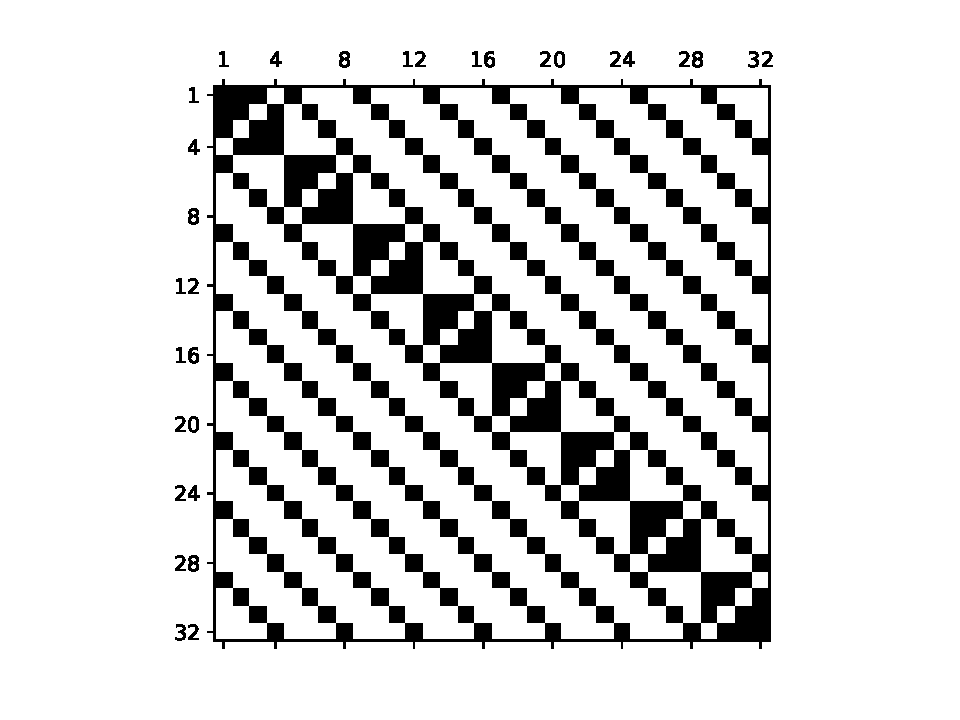
\includegraphics[width=.9\textwidth]{figures/therefore_figs/spy.pdf}
    \caption{Sparsity pattern of a two group, four angle OCI $\bm{A}_j$ system generated for each cell.}
    \label{fig:spyA}
\end{figure}

Figure~\ref{fig:spyA} shows the structure of the within-cell system of equations arises from a two-group four-angle problem.
While $A_j$ does have significant sparsity, with an occupancy ratio of
\begin{equation}
    O_c = \frac{G(N+2)}{4NG} 
    \; ,
\end{equation}
which approaches 25\% with large angular and group counts, in this work we use dense representations in each cell because the matrix memory size for 1D transport is not limiting.

\subsection{Implementation on GPUs}

Implementing the OCI and SI approaches on GPUs requires a numerical linear algebra solver library like LAPACK~\cite{laug}.
Many high-performance open-source linear algebra tools exist (e.g., Trillinos \cite{trilinos-website}, PETSc \cite{petsc-user-ref}, MAGMA \cite{magma}), but we chose a vendor-supplied package depending on the hardware target of choice.
Our target hardware is an AMD MI250X so we use the AMD ROCm compute library to solve the system of equations.
Modern GPU vendor-supplied LAPACK libraries often include a \texttt{batched} class of solvers,
which operate on a group of like-sized systems in unison and are optimized by the hardware vendors.
For example, LU decomposition with pivoting (a generic direct solver for a system of linear equations) used in this work, comes from RocSolver's \texttt{strided\_batched\_dgesv} \cite{rocsolver}.

We use direct solvers here because all systems are relatively small, with orders ranging between 4 and 100.
This makes the use of a batched implementation of LU decomposition with pivoting ideal.
Furthermore, LAPACK-type implementations of \texttt{\_gesv} (\textbf{GE}neral linear \textbf{S}ol\textbf{V}e)  automatically return the $L+U+D$ decomposition of a generic matrix $A$.
So, in subsequent iterations, this system can be back solved quickly (using LAPACK \texttt{\_getrs}).
In this mode for both SI and OCI, the only user-defined device kernels are the RHS vector builders which are already memory safe operations.

This software engineering design will increase the memory footprint of OCI and SI as the $LHS$ matrices are stored in memory.
This is acceptable for 1D transport but more optimization may be required when moving to 2D and 3D solvers.

Algorithm \ref{alg:si} describes the convergence loop for source iteration.
$\mathbf{L}_{c,j,g,m}$ and $\bm{d}_{j,g,m}$ matrices are always of dimension $4\times 4$ and 4, respectively, for our space time-discretization scheme and are defined in Appendix~\ref{app:source_iteration}.
The number of systems to solve changes with the number of angles ($N$), groups ($G$), and cells ($J$).
In this algorithm the number of systems solved in parallel at one spatial index $j$ is $N \times G$.
SI requires host-side dispatching in every cell to execute the sequential nature of the sweep.
We implemented this algorithm to do all available computing at once (negative sweeps are happening in unison with positive ones in all angles and groups).
The angle parallelism exploited for this implementation of SI on the GPU is enabled by the \texttt{strided\_batched} call itself.
Thus, the traditional loop over all angles is implemented by the solver, not explicitly by the user.
Group-to-group communication is done at the end of every iteration.
The first iteration calls the full \texttt{\_gesv} algorithm, which returns the solution of the system and the $L+U+D$ decomposition in $A$.
Subsequent iterations just perform a back substitution (\texttt{\_getrs}).
Profiling shows that host functions (including host$\rightarrow$device and device$\rightarrow$host communication) account for up to around $9\%$ of the runtime in the largest problems we considered.

\begin{algorithm}
\begin{algorithmic}[1]
    \State build $\mathbf{L}_{c,j,g,m}$ for each cell, angle, and group \Comment{Eq. \ref{eq:app:si_sys}}
    
    \State move $\mathbf{L}_{c,j,g,m}$ to device

    \State $\beta$ = $4NG$ \Comment{offset to a cell} %\Comment{offset to a cell}

    \State $l = 0$ \Comment{iteration counter}

    \State converged = false

    \While{!converged}

    \State build constant part of $\bm{d}_{j,g,m}$ in all cells, angles, and groups \Comment{Eq. \eqref{eq:app:si_rhs}}

    \State move constant part of $\bm{d}_{j,g,m}$ to device
        
        \For{j = 0 to $J$ } \Comment{parallel over groups and angles}

            \State build variable part of $\bm{d}_{j,g,m}$ at cells $j$ and $J-j$  \Comment{on GPU Eq. \eqref{eq:app:si_rhs}}

            \If{l=0}
                \Comment{LHS in, L+U+D out}
                \State $\Psi_j$ = \texttt{GPU\_strided\_batched\_dgesv}($\mathbf{L}_{c,j}$[$\beta^{2}j$],$\bm{d}_{j}$[$\beta j$])
            \Else
                \Comment{back substitution}
                \State $\Psi_j$ = \texttt{GPU\_strided\_batched\_dgetrs}($\mathbf{L}_{c,j}$[$\beta^2j$],$\bm{d}_{j}$[$\beta j$]) 
            \EndIf
        \EndFor

        \State move $\Psi$ to Host

        \State $\bm{\phi}^l =\sum_{n=1}^{N} w _n\Psi^{l}_{n}$ \Comment{Eq. \eqref{eq:app:si_sf}}

        \State $e=||\bm{\phi}^l - \bm{\phi}^{l-1}||_2$

        \State $\rho_e = e^l / e^{l-1}$

        \If{$e < \epsilon(1-\rho_e)$}
            converged = true
        \EndIf

        \State $e^{l-1} = e^l$ 

        \State $l++$
        
        \State move $\Phi^l$ to Host

        \State communicate group to group \Comment{Eq. \eqref{eq:app:si_update}}

    \EndWhile
    \vspace{1.5em}
    \caption{Source iteration algorithm implemented on GPU where $\bm\phi$ is scalar flux. Equations in Appendix~\ref{app:source_iteration}. Simplified for brevity.}
    \label{alg:si}
\end{algorithmic}
\end{algorithm}

Algorithm \ref{alg:ocigpu} describes OCI's on-GPU convergence loop.
We found OCI to be more sensitive to within-iteration optimizations.
In some cases (specifically in the thin limit) OCI may require significantly more iterations to converge.
For that reason, it is imperative that the OCI iteration take place entirely on the GPU.
Luckily, OCI's algorithm is simpler to implement on GPUs because group-to-group communication happens within the solved systems.
We implemented the following algorithm to do that: everything under the \texttt{while} loop is wholly contained on the GPU, requiring minimal device-to-host communication.

\begin{algorithm}
\begin{algorithmic}[1]
    \State build $\bm{A}_j$ in all cells and move to device \Comment{Eq.~\eqref{eq:fullOCIlhs}}

    \State build constant part of $\bm{b}_j$ in all cells and move to device \Comment{Eq.~\eqref{eq:fullOCIrhs}}

    \State $l = 0$ \Comment{iteration counter}

    \State converged = false

    \While{converged}
        \Comment{incident angular fluxes from previous iteration}
        
        \State build variable part of $\bm{b}_j$ in all cells \Comment{user-defined GPU kernel, Eq.~\eqref{eq:fullOCIrhs}}

        \If{l=0}
            \Comment{A in-out becomes the L+U+D decomp}
            \State $\Psi$ = \texttt{GPU\_strided\_batched\_dgesv}($A$,$b$)
        \Else
            \Comment{back substitution}
            \State $\Psi$ = \texttt{GPU\_strided\_batched\_dgetrs}($A$,$b$) 
        \EndIf

        \State $e=||\Psi^l - \Psi^{l-1}||_2$ \Comment{Done on GPU using rocBLAS dr2n}

        \State $\rho_e = e^l / e^{l-1}$ \Comment{spectral radius estimation}

        \If{$e < \epsilon(1-\rho_e)$} \Comment{controlling for false convergence}
            \State converged = true
        \EndIf

        \State $e^{l-1} = e^l$

        \State $b^{l-1} = b^l$

        \State $l++$
            
    \EndWhile
    
    \State move $\Psi$ to host
    \caption{One-cell inversion algorithm implemented on GPUs. Simplified for brevity.}
    \label{alg:ocigpu}
\end{algorithmic}
\end{algorithm}

OCI's systems are represented as dense within a cell and built in a strided-batched configuration to take advantage of the block sparsity.
However, now systems within an iteration can be dispatched in unison.
Just as with the SI algorithm, the GPU strided batched solver implements the parallel loop over all cells.
The intra-iteration $b$-vector production kernels are the only user-defined device functions required in this algorithm. These are relatively simple to implement as they are thread-safe operations.


\section{Results}
\label{sec:results}

In this section, we show results that support our initial conjecture that OCI convergence accelerates, more than SI, in transient transport calculations with decreased time step sizes.
We also further analyze OCI's performance on AMD MI250X GPUs using batched LAPACK solvers on a highly scattering problem from literature at multiple time step sizes and cell width values.

\subsection{Fourier analysis: transient iterative convergence rate}
\label{sec:results-faoci}

To study the impact of transient conditions on OCI we solve the Fourier system for steady-state and time-dependent transport derived in Section~\ref{sec:methods-faoci} both for simple corner balance in space.
For all Fourier analyses we sample $\lambda \in [0,2\pi]$ at \num{250} points and use \texttt{numpy.max(numpy.abs(numpy.eig(}$T$\texttt{)))} to compute spectral radius at a given point in parameter space ($\delta$ ($\Sigma\Delta x$), $\tau$ ($\Sigma v\Delta t$), and $c$ ($\Sigma_s$/$\Sigma$)) in S$_{8}$ using Gauss--Legendre quadrature.

Table~\ref{table:difflimit} shows spectral radii produced from steady-state and transient OCI systems with various choices of mean free time ($\tau$), at various cellular optical thicknesses ($\delta$).
Steady-state predictions show the expected and previously published results that $\rho=1$ when $c=1$ regardless of $\delta$.
However, for the time-dependent system, $\rho<1$ regardless of the considered $\tau$ and $\delta$.
Furthermore, as $\tau$ shrinks and $\delta$ grows, $\rho$ dramatically decreases, approaching zero at the smallest $\tau$ and largest $\delta$.

\begin{table}
  \centering
  \begin{tabular}{@{}l c c c @{}} \toprule
    $\tau$ & $\delta=10.$ & $\delta=1.0$ & $\delta=0.1$ \\ \midrule
    SS  & \num{1.0000} & \num{1.0000} & \num{1.0000} \\
    10 & \num{0.99522} & \num{0.99952} & \num{0.99995} \\
    1  & \num{0.95323} & \num{0.99522} & \num{0.99952} \\
    0.1   & \num{0.64031} & \num{0.95321} & \num{0.99522} \\
    0.01 & \num{0.11177} & \num{0.63343} & \num{0.95351} \\
    \bottomrule
  \end{tabular}
  \caption{OCI spectral radius $\rho$ in the diffusive limit ($c=\Sigma_s/\Sigma =1.0$) from Fourier analysis at various mean free time ($\tau$) and cellular optical thickness ($\delta$) values. SS indicates steady state.} 
  \label{table:difflimit} 
\end{table}

Figure~\ref{fig:specrad_fa} shows $\rho$ predictions for OCI and SI produced from the Fourier system.
As previously published: as $\delta$ gets smaller, $\rho$ approaches 1 regardless of the scattering ratio.
As postulated in this work: as $\Delta t$ gets smaller, $\rho$ tends to 0---due to improvements in scattering ratio (which also affects SI) and increasing $\delta$---increasing the diagonal dominance of the iteration matrix.

\begin{figure}
    \centering
    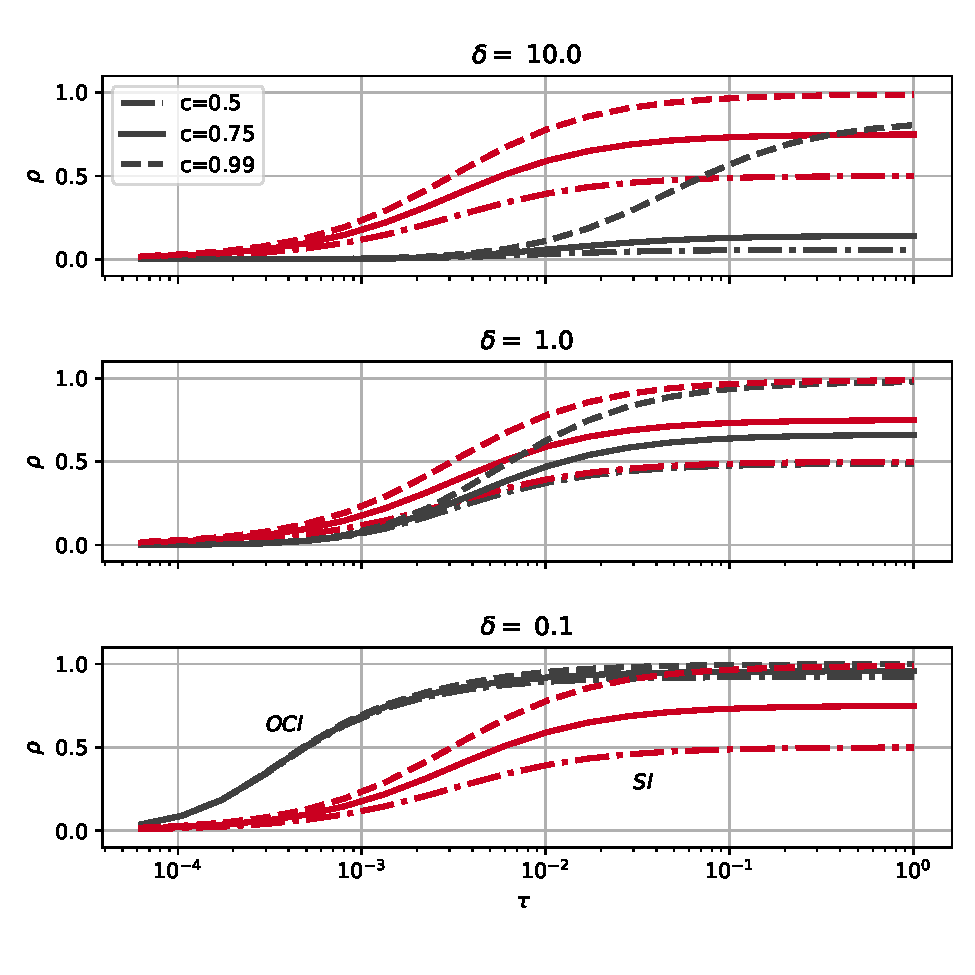
\includegraphics[width=\textwidth]{figures/therefore_figs/spec_rad_over_dt.pdf}
    \caption{Spectral radius of OCI (black) and SI (red) over choices of mean free path ($\delta$), time step ($\Delta t$), and scattering ratio ($c$).}
    \label{fig:specrad_fa}
\end{figure}

Fourier analysis results also show that, depending on the location in parameter space, the dominant eigenvalue ($|\lambda_{max}|$) can have large imaginary components, with positive or negative real components and complex conjugate reflections over the real axis.
Complex dominant eigenvalues leading to oscillatory convergence patterns have previously been identified in spatial domain decomposition algorithms where $\rho=1$ when $\delta \rightarrow 0$ \cite{compeig2019ani}. 

Deterministic solvers are commonly verified against predictions of $\rho$ from Fourier analysis.
We attempted to do the same by running a problem with length \SI{100}{\centi\meter}, vacuum boundary conditions, a convergence tolerance of \num{1e-13}, $\Sigma=$ \SI{2.5}{\per\centi\meter}, $\Delta x=$ \SI{0.10}{\centi\meter}, $c=$ \num{0.9}, $\Delta t=$\SI{0.10}{\s}, $v=$ \SI{4.0}{\meter\per\s} ($\delta =$ \num{0.25}, $\tau=$ \num{1.0}), a random (uniform [0,1]) initial guess for the angular flux, and no material source in S$_8$.
The random initial guess excites all error modes and provides an anaclitic solution ($\Psi^{\text{converged}} = \bm{0}$) to compute iteration errors.
Figure \ref{fig:eigplot} on the left shows the predicted eigenvalues from Fourier analysis and indicates the dominant eigenvalue that contributes to $\rho$ for this particular problem.
In this case, that dominant eigenvalue has considerable real and complex components at $\lambda_{max} =$ \num{0.429} $+$ \num{0.216}$i$ and $\rho=$ \num{0.4831}.

Figure~\ref{fig:eigplot} on the right shows $\rho$ predicted from Fourier analysis (flat constant line) as well as $\rho$ measured from the ratio of subsequent residuals as a function of iteration count ($l$).
The empirically estimated value of $\rho$ oscillates around the predicted spectral radius until convergence, with a measured amplitude around \num{0.1}.
The oscillation of the empirically measured spectral radius also seems to grow through iteration count, which may be due to the compounding impact of truncation error and/or machine precision.
So, we cannot rigorously verify our implementation of OCI via Fourier results, because only a mean of the oscillation will match the only-real $\rho$ provided from Fourier results ($|\lambda_{max}|$).
More work is warranted to develop methods that can better capture the empirical behavior of the ratio of subsequent residuals produced from a transport solver and relate them to the complex dominant eigenvalues that may be predicted from Fourier analysis.

\begin{figure}
    \centering
    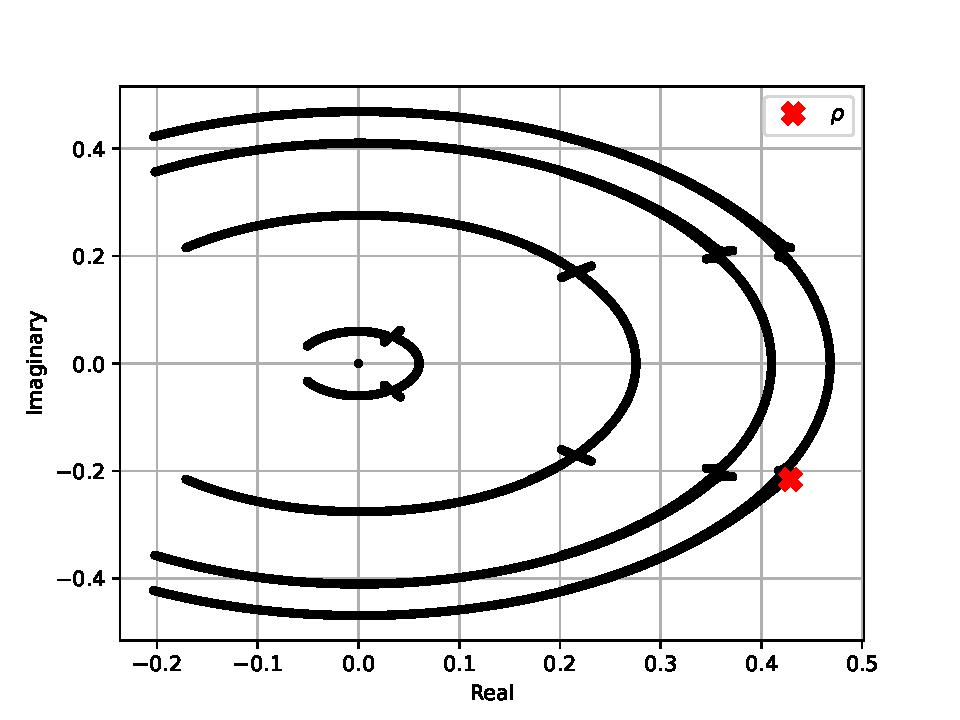
\includegraphics[width=.49\textwidth]{figures/therefore_figs/eig_plot.pdf}
    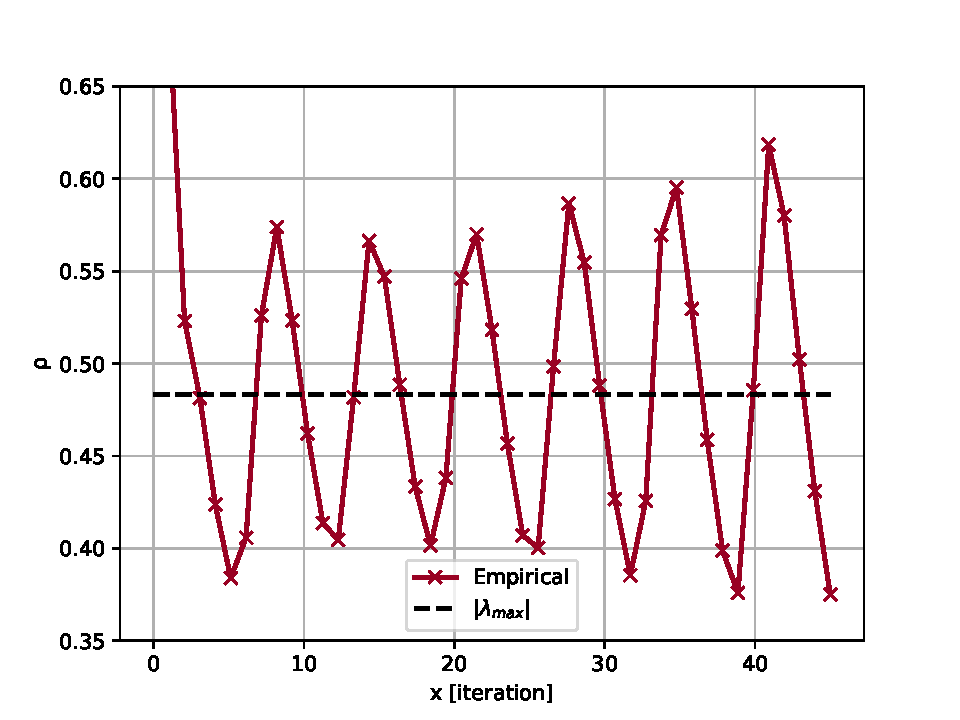
\includegraphics[width=.49\textwidth]{figures/therefore_figs/eig_spec_rad.pdf}
    \caption{Eigenvalues in the complex plane of OCI (left), and spectral radius as a function of iteration from the empirical ratio of subsequent residuals and as predicted by Fourier analysis (right).}
    \label{fig:eigplot}
\end{figure}

\subsection{Performance on GPUs}

Runtime results were gathered on the Tioga machine at Lawrence Livermore National Laboratory.
Tioga is an early access machine for LLNL's exascale-class El Capitan machine.
On its standard partition, Tioga's nodes have four AMD MI250X GPUs and one AMD EPYC 7A53 CPU.
Our methods are currently implemented for a single GPU, so this analysis will be limited to using a single graphics compute die of an MI250X.
We compiled using ROCm version 6.2.1 (includes rocSOLVER and rocBLAS libraries) and used double precision for all values represented.

To analyze performance, we adapt a test problem described by \cite{rosa_cellwise_2013} for a 1D time-dependent, multi-group problem.
Table~\ref{table:rosa_test} describes the material data for this 
two-group problem ($L=$ \SI{100}{\centi\meter}) with vacuum boundary conditions on either side. 
The initial condition is $\psi_{t=0} = 0$, and we analyze runtime performance over various choices of $\delta$ and quadrature order at time step sizes of $\Delta t=$ \SI{0.1}{\s} and \SI{10.0}{\s}.
The problem is highly scattering with a maximum scattering ratio of \num{0.99997}.


\begin{table}
  \centering
  \begin{tabular}{@{}c c c c c c@{}} \toprule
    Property & Group 1 & Group 2 & units \\ \midrule
    $\Sigma$ & 1.5454 &  0.45468 & cm$^{-1}$  \\
    $\Sigma_{s,g\rightarrow g}$  & 0.61789 &  0.0072534 & cm$^{-1}$  \\
    $\Sigma_{s,g'\rightarrow g}$  & 0.38211 &  0.92747 & cm$^{-1}$ \\
    $\Sigma_s/\Sigma$ & 0.99997 & 0.86012 & - \\
    $Q$ & 1 & 1 & cm$^{-3}$s$^{-1}$\\
    $v$ & 1 & 0.5 & cm s$^{-1}$ \\
    \bottomrule
  \end{tabular}
  \caption{Test problem material data and simulation parameters.}
  \label{table:rosa_test} 
\end{table}

Figure~\ref{fig:runtimes10.0} on the left compares the wall clock runtime of OCI (in black) and SI (in red) over various selections of $\delta$ (controlled via $\Delta x$) with $\Delta t=$ \SI{10.0}{\s}, Figure~\ref{fig:runtimes10.0} on the right shows the speedup of OCI over SI.
In each row, we are increasing quadrature order to increase the overall dimensionality of the system.
Figure \ref{fig:runtimes0.1} shows the same information, but for $\Delta t=$ \SI{0.1}{\s}.
Runtimes are measured over the convergence loops (see Algorithms \ref{alg:si} and \ref{alg:ocigpu}), so do not include the building and moving the $A_j$ matrices from host to device.
The total cross section used in the $\delta$ scale is the limiting value (the smallest) from group 2 (see Table \ref{table:rosa_test}).

SI's convergence loop runtime increases linearly as cellular optical thickness decreases as there are more cells to solve  in serial.
The number of iterations required to converge the solution is the same but the size of the solution grows.
SI only has $NG$ $4\times4$ systems to solve at any moment so the amount of serial work increases with the number of cells (decreasing $\delta$).
However, as we increase quadrature order the runtime performance of SI actually improves because the solver has more parallelizable degrees of freedom.

\begin{figure}
    \centering
    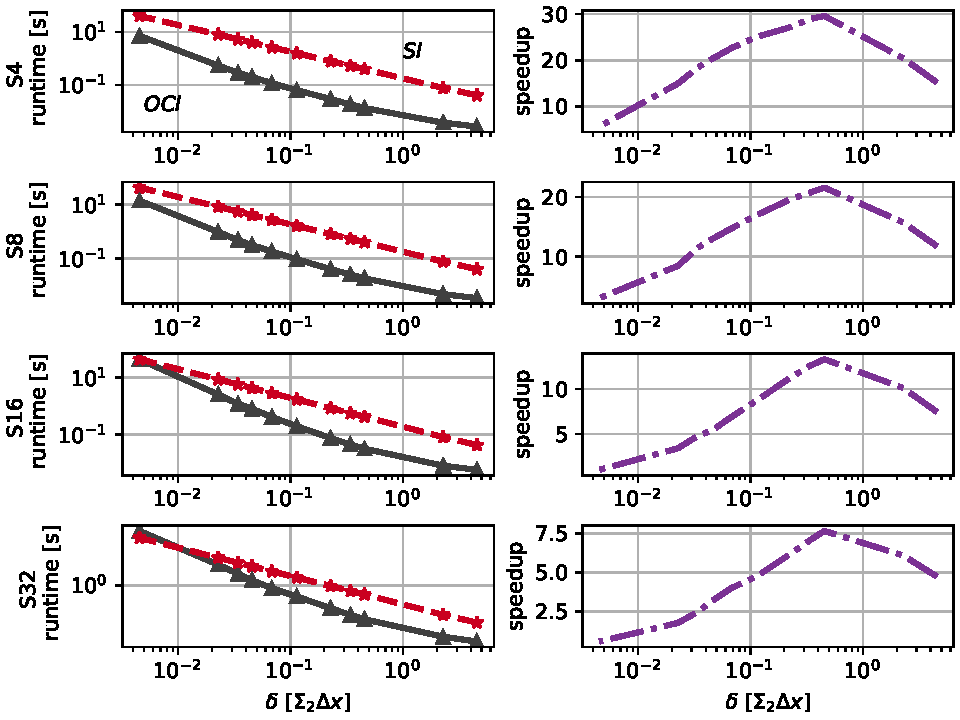
\includegraphics[width=1.0\textwidth]{figures/therefore_figs/runtimes_10.0.pdf}
    \caption{Wall-clock runtimes of the convergence loop (left) and 
    speedup of OCI over SI (right) at $\Delta t=$\SI{10.0}{\s} ($\tau=$ \num{2.2734}) as a function of $\delta$ and at various quadrature orders.}
    \label{fig:runtimes10.0}
\end{figure}

\begin{figure}
    \centering
    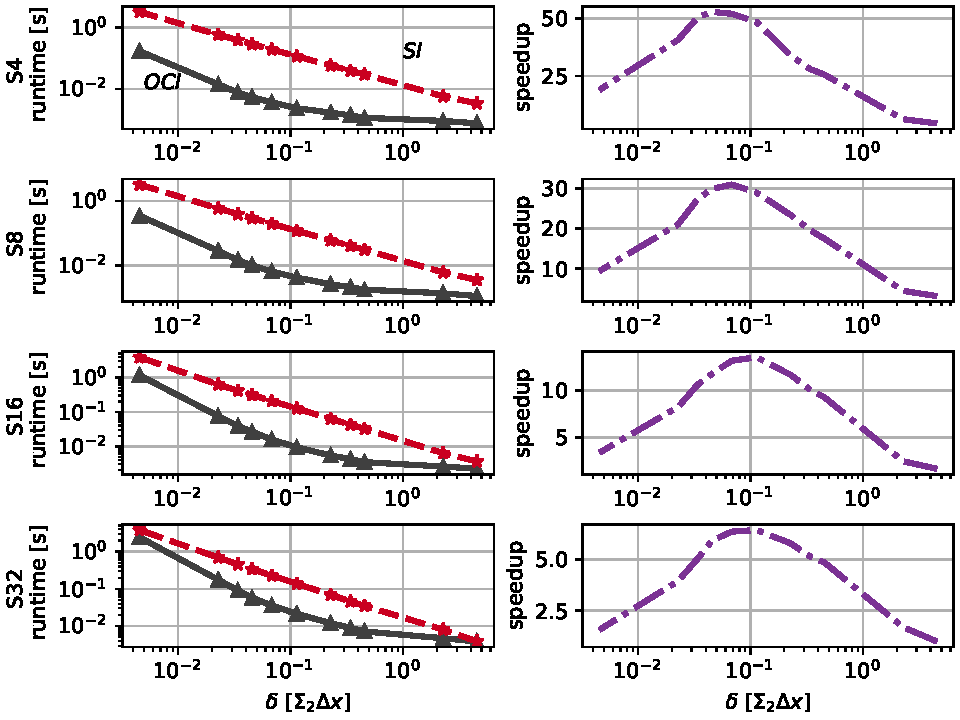
\includegraphics[width=1.0\textwidth]{figures/therefore_figs/runtimes_0.1.pdf}
    \caption{Wall-clock runtimes of the convergence loop (left) and 
    speedup of OCI over SI (right) at $\Delta t=$\SI{0.1}{\s} ($\tau=$ \num{0.0227}) as a function of $\delta$ and at various quadrature orders.}
    \label{fig:runtimes0.1}
\end{figure}

For larger time steps, OCI shows less speed-up over SI as it slows for S$_{16}$ and S$_{32}$ quadratures in the thin limit.
The parallelizable degrees of freedom increase with the number of cells (by decreasing $\delta$), but the spectral radius decreases dramatically as cells get thinner.
In the thin limit, OCI requires more iterations to converge the solution, but those iterations can be done faster on the GPU than with SI.
OCI seems to have a ``sweet spot'', where the size of the matrices is optimal for the solver, before the spectral radius degrades in the thin limit.
This is observed at around $\delta=4$ for $\Delta t=$ \SI{10}{\s} and $\delta=0.1$ for $\Delta t=$ \SI{0.1}{\s}.
The location of this optimality depends on factors including optimizations at the solver level employed when compiling the vendor-supplied LAPACK libraries \cite{rocsolver}.
The smaller time step increases OCI's relative performance over SI, generally increasing speedup by upwards of 40\% for this highly scattering problem.

\section{Discussion}

% transient patterns 
The 1D convergence trends we present here agree with
previously published 2D steady-state Fourier results for OCI schemes 
(i.e., $\rho\rightarrow1$ as $\delta\rightarrow0$) \cite{rosa_cellwise_2013, man1994parallel}.
This leads us to expect that the relationship between mean free time and spectral radius will persist in higher spatial dimensions, 
but exactly how much dynamic impacts to OCI decrease $\rho$ in 2D transport has yet to be shown.

% preconditioned FPS v OCI in 3D
Parallel sweeping algorithms may not be well suited to GPUs where non-uniform work distributions come with significant overhead. 
Available results for full parallel sweeps on GPUs show that even optimized applications underperform relative to the theoretical hardware resources available \cite{Thomas_2024_profiling, wolfe2022roofline, kunen_kripke_2015, womeldorff_taking_2017, zerr_partisn_2019}.
On the other hand, space-parallel OCI uses the same parallel scheme in 2D and 3D as it does in 1D, with arithmetically intense operations that align well with the GPU parallelism paradigm.
So, we hypothesize that OCI can better take advantage of the compute resources available on GPUs in higher dimensions than full-parallel-sweep SI on GPUs, but this requires further study.

Production SI codes that simulate high-fidelity 3D models never form the actual iteration matrix, resulting in significant memory efficiency~\cite{partisn, evans_denovo_2010, kunen_porting_2019, MINARET, wang_necp_hydra_2020, ShemonEmilyR.2016PUM}.
Our implementation of OCI is not memory efficient, because we store the strided batched representation of the entire linear system for the iteration algorithm.
While this block-sparse representation does dramatically save memory, more optimizations to OCI may be needed when moving to 3D.
For example, OCI forms the iteration matrix as a linear operator.
Many algorithms exist to solve systems of linear operators without ever forming the matrix.
Libraries already exist to do this on CPUs and GPUs (e.g., LibCEED \cite{libceed-joss-paper}).
Even more simple optimization may involve using sparse representations for the cell blocks themselves and sparse direct solvers.


OCI algorithms may be better suited for domain-decomposed simulations (required for distributed-memory parallelism) than SI.
Some KBA algorithms can degrade with large processor counts \cite{baker_kba_2017}.
For a hypothetical OCI algorithm, communication between subdomains can be very organized, occurring at every iteration (or after a specified number of iterations) at the same time as all other subdomains.
This may lead to superior weak scaling across large decomposed problems on distributed (MPI) type systems.
Many parallel domain decomposition algorithms are already based on the same underlying parallel block Jacobi, Gauss--Seidel, or red-black iterations as OCI \cite{anistratov_iterative_2015, compeig2019ani}.

While this work is limited to AMD GPUs and the ROCm software stack, our implementation of OCI is portable to other GPU types.
In fact, the workflow present in OCI---solving many small dense or sparse linear algebra systems in parallel---is common in much numerical software.
We expect that these types of solvers will exist when porting to a new hardware accelerator used for scientific computing.
For example, Nvidia's cuSOLVER \cite{cuSovler} and Intel's oneMKL \cite{oneMKL} both implement strided batched versions of LU decomposition with pivoting for their GPUs.
Porting the OCI algorithm presented in Algorithm~\ref{alg:ocigpu} to another GPU would just require altering names of solver function calls, compiler commands, and switching out library header imports.

OCI algorithms may also be well suited for modeling anisotropic scattering distributions because all angles are computed at once in every cell.
On unstructured meshes, OCI algorithms avoid one challenge for sweep-based methods: when groups of cells have cyclic dependencies (i.e., when an incident transport angle is parallel to a cell boundary).

% OCI's need for a perfomant preconditioner
Regardless of how well an implementation of any OCI scheme performs, the inability to converge problems in the thin limit regardless of scattering ratio will continue to lead to lackluster performance in some problems.
In this work, we compared unpreconditioned SI to unpreconditioned OCI using fixed-point iterations.
When in production, SI typically uses a well-accepted set of acceleration schemes/preconditioners (most popularly diffusion synthetic acceleration) accompanied by Krylov subspace methods.
Likewise, some acceleration/preconditioning or Krylov methods may exist that can help OCI more-rapidly converge in the thin limit, while not significantly degrading the space-parallel performance of OCI.

Acceleration schemes for OCI have previously been explored, including transport synthetic acceleration \cite{tsa2009rosa} and using hybrid schemes with OCI and traditional SI \cite{hoagland_hybrid_2021}.
Both resynchronize cells by sweeping to improve convergence; however, the resulting algorithms are no longer space-parallel and involve a potentially more-expensive sweep operation.

\section{Conclusions and Future Work}

We derived the multiple balance and simple corner balance time-space discretization schemes and demonstrated, with Fourier analysis, that our time iteration method is unconditionally stable.
We also derived eigensystems for one-cell inversion and source iteration, showing that one-cell inversion iterations converge faster as mean free time shrinks.
Furthermore, OCI's convergence rate improves faster than SI's with decreasing mean free time.
We confirmed this with both Fourier and empirical analysis of implemented one-cell inversion and source iteration solvers.
Although we only explored block Jacobi OCI, we also expect this behavior to improve convergence of time-dependent block Gauss--Seidel OCI.

When more iterations are required to converge problems of interest---particularly in highly scattering and optically thin problems---OCI can run individual iterations significantly faster than SI when using batched direct solvers on GPUs from vendor-supplied libraries.
For OCI the number of on-device performant compute kernels is limited to data-parallel matrix-building operations, with all other compute kernels being called from optimized libraries. 
While optimization could improve both the OCI and SI algorithms, we analyzed performance to ensure there was little computational overhead from data movement and user-defined kernels.

Moving forward, we are exploring synthetic acceleration techniques to preserve the OCI space-parallel performance on GPUs while ameliorating issues in the thin and scattering limits.
Space-parallel OCI schemes offer promise as a high-performing class of iterative solvers for time-dependent radiation transport on modern heterogeneous compute architectures.

\section*{Acknowledgments}

The authors thank Dmitriy Anistratov of North Carolina State University for useful conversations about Fourier analysis results, James Warsa of Los Alamos National Laboratory for useful conversations about previous work and Damon McDougall of Advanced Micro Devices for support using ROCm compilers and profilers. 
The authors also thank the high performance computing staff at Lawrence Livermore National Laboratory for support using the Tioga machine.

This work was supported by the Center for Exascale Monte Carlo Neutron Transport (CEMeNT), a PSAAP-III project funded by the Department of Energy, grant number: DE-NA003967.

\section*{Appendix: Source Iteration Systems}
\label{app:source_iteration}

\newcommand{\lph}{^{(l+1/2)}}
\newcommand{\lp}{^{(l+1)}}


Using a source iteration to solve a multi-group problem with multiple balance in time \cite{variansyah_robust_2021} and simple corner balance in space \cite{adams_subcell_1997} gives a $4\times 4$ system of linear equations:
\begin{equation}
    \label{eq:app:si_sys}
    \mathbf{L}_{c,j,g,m} \begin{bmatrix}
    \psi_{m,k,g,j,L}\lph \\
    \psi_{m,k,g,j,R}\lph \\
    \psi_{m,k+1/2,g,j,L}\lph \\
    \psi_{m,k+1/2,g,j,R}\lph
    \end{bmatrix}
    = \mathbf{d}_{j,m,g} \;,
\end{equation}
solved in every angle and group by sweeping from cell to cell,
where $\mathbf{L}_{c,j,g,m}$ is from Eq. \eqref{eq:Aj}
and
\begin{subequations}
\label{eq:app:si_rhs}
\begin{equation}
    \mathbf{d}_{j,g,m} = 
    \begin{cases}
        \bm{d}_{j,g,m}^+ & \mu_m>0 \\
        \bm{d}_{j,g,m}^- & \mu_m<0 \\
    \end{cases} \;,
\end{equation}
where
\begin{equation}
   \bm{d}_{j,g,m}^+ = \begin{bmatrix}
    \frac{\Delta x_j}{4} \left( \Sigma_{s,g\rightarrow g,j} \phi_{k,g,j,L}^{(l)}  +   Q_{k,j,L} \right) + \frac{\Delta x_j}{2 v_g \Delta t} \psi_{m,k-1/2,g,j,L} + \mu_m \psi_{m,k,g,j-1,R}\lph \\
    \frac{\Delta x_j}{4} \left( \Sigma_{s,g\rightarrow g,j} \phi_{k,g,j,R}^{(l)}  +   Q_{k,j,R} \right) + \frac{\Delta x_j}{2 v_g \Delta t} \psi_{m,k-1/2,g,j,R} \\
    \frac{\Delta x_j}{4} \left( \Sigma_{s,g\rightarrow g,j} \phi_{k+1/2,g,j,L}^{(l)}  +   Q_{k+1/2,j,L} \right) + \mu_m \psi_{m,k+1/2,g,j-1,R}\lph \\
    \frac{\Delta x_j}{4} \left( \Sigma_{s,g\rightarrow g,j} \phi_{k+1/2,g,j,R}^{(l)}  +   Q_{k+1/2,j,R} \right) 
    \end{bmatrix} \;,
\end{equation}
\begin{equation}
   \bm{d}_{j,g,m}^- = \begin{bmatrix}
    \frac{\Delta x_j}{4} \left( \Sigma_{s,g\rightarrow g,j} \phi_{k,g,j,L}^{(l)}  +   Q_{k,j,L} \right) + \frac{\Delta x_j}{2 v_g \Delta t} \psi_{m,k-1/2,g,j,L}  \\
    \frac{\Delta x_j}{4} \left( \Sigma_{s,g\rightarrow g,j} \phi_{k,g,j,R}^{(l)}  +   Q_{k,j,R} \right) + \frac{\Delta x_j}{2 v_g \Delta t} \psi_{m,k-1/2,g,j,R} - \mu_m \psi_{m,k,g,j+1,L}\lph  \\
    \frac{\Delta x_j}{4} \left( \Sigma_{s,g\rightarrow g,j} \phi_{k+1/2,g,j,L}^{(l)}  +   Q_{k+1/2,j,L} \right)  \\
    \frac{\Delta x_j}{4} \left( \Sigma_{s,g\rightarrow g,j} \phi_{k+1/2,g,j,R}^{(l)}  +   Q_{k+1/2,j,R} \right) - \mu_m \psi_{m,k+1/2,g,j+1,L}\lph
    \end{bmatrix} \;,
\end{equation}
and $\phi$ is the scalar flux.
\end{subequations}
After sweeping the mesh cells in the appropriate directions for each angle in the quadrature set and every group, the scalar flux vector can be updated via
\begin{equation}
\label{eq:app:si_sf}
\bm{\phi}_{k,g,j}\lph = 
\begin{bmatrix}
    \phi_{k,g,j,L}\lph \\
    \phi_{k,g,j,R}\lph \\
    \phi_{k+1/2,g,j,L}\lph \\
    \phi_{k+1/2,g,j,R}\lph
    \end{bmatrix}   = \sum\limits_{n=1}^N w_n 
    \begin{bmatrix}
    \psi_{n,k,g,j,L}\lph \\
    \psi_{n,k,g,j,R}\lph \\
    \psi_{n,k+1/2,g,j,L}\lph \\
    \psi_{n,k+1/2,g,j,R}\lph
    \end{bmatrix} \;.
\end{equation}
Then, group-to-group communication can be computed with
\begin{equation}
    \label{eq:app:si_update}
    \bm{\phi}_g\lp = \bm{\phi}_g\lph + \sum_{g'\neq g} \Sigma_{s, g'\rightarrow g } \bm{\phi}_{g'}\lph \; .
\end{equation}
Note that within group scattering is computed in the transport sweep itself, in Eq.~\eqref{eq:app:si_rhs}.
This algorithm allows for all groups and angles to be solved in parallel (using a Jacobi iteration). 
This algorithm gives source iterations the greatest number of degrees of freedom to parallelize for a 1D, slab geometry, multi-group problem---the best case scenario for GPU performance.
\begin{subequations}
Then, the source iteration can continue until 
\begin{equation}
    ||\bm{\phi}^{(l+1)}-\bm{\phi}^{(l)}||_{2} < \epsilon(1-\rho_{e,SI}) \; ,
\end{equation}
where $\epsilon$ is the convergence tolerance and
\begin{equation}
    \rho_{e,SI} = \frac{||\bm{\phi}^{(l+1)}-\bm{\phi}^{(l)}||_{2}}{||\bm{\phi}^{(l)}-\bm{\phi}^{(l-1)}||_{2}} \; ,
\end{equation}
\end{subequations}
is an empirical estimation of the spectral radius computed at every iteration of a transport solve. 
After converging, the simulation can move to the next time step.
\newpage
\renewcommand{\TheTitle}{Efficient Preconditioning for Space-Parallel One Cell Inversions in Slab Geometry using a Second Moment Method}
\renewcommand{\TheAuthors}{Joanna Piper Morgan,
  Todd S. Palmer,
  Ilham Variansyah, and
  Kyle E. Niemeyer}

\renewcommand{\TheAddress}{
    \textit{In preparation for submission to\\Journal of Computational and Theoretical Transport}
}

\PaperHeader{\TheTitle}{\TheAuthors}{\TheAddress}

\chapter{\TheTitle}
\label{chap:smom_paper}

\epigraphhead[10]{\singlespacing
    \epigraph{
        \emph{hic svnt dracones}
    }
    {Hunt–Lenox Globe}
}


\newcommand{\dxt}{\frac{\Delta x_j}{2}}
\newcommand{\mum}{\mu_m}

\newcommand{\Lc}{\bm{L}_c}
\newcommand{\Lb}{\bm{L}_b}

\newcommand{\scat}{\sigma_s}
\newcommand{\tot}{\sigma}
\newcommand{\abs}{\sigma_a}

\newcommand{\la}{^{(l)}}

\newcommand{\af}{\psi}
\newcommand{\sfl}{\phi}
\newcommand{\smom}{\Gamma}
\newcommand{\fmom}{J_\pm}
\newcommand{\fmomp}{J_+}
\newcommand{\fmomn}{J_-}

\newcommand{\ddx}{\frac{\partial}{\partial x}}
\newcommand{\ddxn}{\frac{d}{d x}}

\newcommand{\sn}{S$_N$}
\newcommand{\pn}{P$_N$}

\newcommand{\half}{\frac{1}{2}}



\section*{Abstract}
Solving the S$_N$ radiation transport equation on modern many cored compute architectures (i.e., GPUs) is challenging.
The most common implemented solution method, the source iteration, requires computational expensive sweeping operations that cannot parallelized in 1D.
While in 2D and 3D sweeps can use full parallel sweeping algorithms these schemes may not perform well on a GPU.
One cell inversion iteration is another class of solvers for the radiation transport equation.
OCI iterations are parallel over spatial cells which has been previously shown to out perform similarly implemented versions of unpreconditioned source iterations on GPUs for some problems.
While OCI is rapidly convergent for optically thick problems spectral radius tends to one in both the optically thin and diffusive limits.
Finding a preconditioner for one cell inversion iterations to support converging in this regime that can be efficiently computed on many-cored architectures motivates this work.
%We have previously shown that for time dependent problems OCI's spectral radius has an added dependence on mean free time and tends to zero as mean free time decreases.
We derive a second moment cellular decomposition method in conjunction with a one-cell inversion iteration in an effort to produce a fully space parallel, rapidly convergent, transport iteration.
The second moment preconditioner derived in this work does not converge to the same solution as unpreconditioned transport solutions suggesting inconsistencies.
Numerical experiments show the second moment preconditioner is rapidly convergent in the thick diffusive limit but dose not aid convergence in the optically thin limit.

\section{Introduction}

The radiation transport equation is a linear partial integro-differential equation that describes the movements of neutral particles (photons, neutron, and neutrinos) in seven independent variables (space, velocity, and time).
Applications of the transport equation include nuclear reactor physics \cite{duderstadt_hamilton}, heat transfer \cite{radheattrans2003}, health physics, and astrophysics.
The transport equation is often solved with either a Monte Carlo or a deterministic method or some kind combination between the two \cite{lewis_computational_1984}.
Monte Carlo methods can be prohibitively slow to converge for high fidelity transient problems; requiring huge numbers of simulated particles to converge to a statistically significant solution \cite{lux_1998}.
Deterministic methods are usually able to reach solution faster for the same problem modeled in similar fidelity, but can be much more sensitive implemented physics and restrictive to what type of problems a particular method can solve \cite{lewis_computational_1984}. 
The high dimensionality of transport equations means that memory and computational efficient iterative methods are often used as a primary solution method \cite{adams_fast_2002}.
As GPUs continue to become the dominant computational workhouse in science and engineering they are allowing for full time dependent solutions to the transport equation.
Finding computationally and memory efficient rapidly convergent numerical methods for modern high performance computers is paramount.

Deterministic methods for the radiation transport equation are commonly divided into in one of two categories: the method of spherical harmonics (\pn) and the method of discrete ordinance (\sn).
Both turn the Boltzmann type intgro-differential transport equation into an infinite set of coupled partial differential equations.
The \pn method does this by taking angular moments of the transport equation then making a closure assumption.
The \sn method, first described Chandrasekhar, treats the double integral over both angular directions with some kind of quadrature discritization \cite{chandrasekhar1960radiative}.
Effectively each differential equation in the infinite set solves along a particular angular direction (in solid angle) provided from quadrature.

\section{Transport Iterations}

Source iterations (SI) are widely used to solve the \sn neutron transport equation \cite{adams_fast_2002}.
The source iteration is a specific operator splitting of the linear neutron transport equation where the scattering term---which couples all \sn ordinates together---is lagged to information from a previous iteration \cite{lewis_computational_1984}.
SI is embarrassingly parallel over angle space which can prove inefficient for large computers as there are usually fewer degrees of freedom in angle than in space.
The SI method requires a transport ``sweep" to spatially move through the problem in a specific non-parallelizable order in 1D.
While memory-efficient parallel 2D and 3D SI schemes exist (namely Koch-Baker-Alcouff (KBA) or full parallel sweeps (FPS) \cite{baker_computational_2017, baker_kba_2017} algorithm), they are difficult to implement and may not be as efficient on GPUs.
Available performance results for full parallel sweeps on GPUs show that even optimized applications under-perform relative to the theoretical hardware resources available \cite{Thomas_2024_profiling, wolfe2022roofline, kunen_kripke_2015, zerr_partisn_2019}.
Finding a rapidly convergent space parallel iteration scheme could prove beneficial to performance on modern many-cored compute architectures (i.e., GPUs).

A one cell inversion iteration (OCI) is an alternative to a source iteration where incident angular fluxes on the surface of the cell are lagged and each cell is solved independently of every other cell \cite{rosa_cellwise_2013, adams_fast_2002}.
Depending on the order of the inversion the iterations can look like a cell-wise block Jacobi, cell-wise block Gauss--Seidel, or red--black iterations \cite{man1994parallel}.
However OCI fails to converge in the thin limit with spectral radius ($\rho$) tending to unity as cellular optical thickness ($\delta=\Sigma\Delta x$ in mean free path) decreases ($\lim_{\delta\rightarrow0}(\rho) = 1$) \cite{tsa_slab2006rosa}.
Physically this can be understood as the requirements of communication from cell-to-cell, information can only pass through a single cell in a single iteration, therefore more cells requires more iterations to communicate information.
Mathematically this is understood as the decreasing diagonal-dominance of the iteration systems present in OCI algorithms, where any fixed point iteration scheme takes longer to converge \cite{isaacson_numerical_1966}.
Previously this has been described as asyncronisity in space \cite{hoagland_hybrid_2021}.
OCI can also become un-convergent in the diffusive or scattering limit.

We have previously shown that on modern GPUs when space is the dominant dimension OCI can out-perform SI in wall clock runtime upto a point in the thin and diffusive limits \cite{morgan2023oci}.
In these circumstances OCI may require more iterations to converge a problem, however, OCI iterations can done much faster on a GPU than similarly implemented SI algorithms.
The OCI algorithm requires the solution to many relatively small linear algebra systems (on the order of 8--100) in each cell; a highly compute bound operation that can be done efficiently on GPUs using library operations \cite{morgan_2025_oci}.
We have also previously shown that adding time resolution to OCI iterations can resynchronize cells and make otherwise unconvergent OCI schemes in the thin and diffusive limit convergent, with spectral radii approaching zero as mean free time decreases \cite{morgan_2025_oci}.
Time resolution is a benefit to convergence for both SI and OCI algorithms however as it is compounding benefit to OCI has an additional dependency on the cellular optical thickness---which is inversely proportional to mean free time.

Figure \ref{fig:ss_spec_rads} shows spectral radii of unpreconditioned SI (left) and unpreconditioned OCI (middle) over choices of cellular optical thickness ($\delta$) and scattering ratio ($c$) computed from Fourier analysis of an infinite homogeneous medium problem in S$_8$\footnote{Gauss-Legendre quadrature is used in all work presented}.
Unprecondtioned source iterations depends linearly on $c$, and for the infinite homogeneous medium problem, does not depend on $\delta$.
OCI depends both on scattering ratio and cellular optical thickness---being rapidly convergent in the thick limit ($\delta>1.0$) with degrading spectral properties towards the thin and diffusive limits ($\delta<1.0$ and $c>0.95$).

\begin{figure}
    \centering
    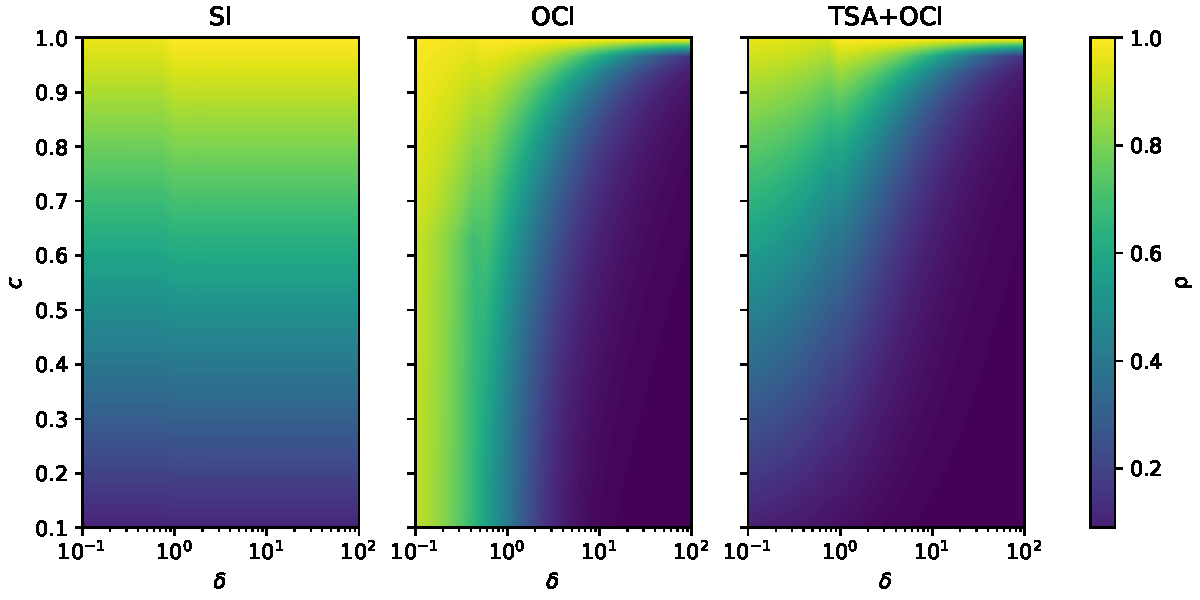
\includegraphics[width=\linewidth]{figures/smm_paper/ss_specrads.pdf}
    \caption{Spectral radii ($\rho$) of (left) unpreconditioned SI, (center) unpreconditioned OCI, and (right) OCI with transport synthetic acceleration ($\beta=1.0$), over ranges of scattering ratio $c$ and cellular optical thickness ($\delta$) in S$_8$ and 200 choices of wave mode $\in[0,2\pi]$. }
    \label{fig:ss_spec_rads}
\end{figure}

Preconditioners can be used to aid convergence of iterative schemes for the neutron transport equation \cite{adams_fast_2002}.
Often physics informed preconditioners for transport iterations may be thought of as high-order method solving the full discretized transport equation and a low-order method informing intra-iteration updates to then be used in the next iteration of the high-order problem.
The low-order method is usually some physics-informed problem that is computationally cheaper to solve then the transport problem and models physical behavior that is difficult for a given operator splitting to converge (e.g., the diffusive limit, $c\rightarrow1$).

Synthetic acceleration schemes are a common subset of preconditioners for the source iteration operator splitting.
A synthetic acceleration method only \textit{accelerates} convergence to the same solution as transport and is fully consistent with the high-order transport method.
Generally for synthetic acceleration methods the low-order simulation is \textit{driven} by the error between iterates of a transport solve.
Synthetic acceleration techniques for source iterations include:
boundary projection acceleration \cite{adams_boundary_1988}, 
transport synthetic acceleration \cite{ramone_1997_tsa},
multi-grid methods \cite{man1994parallel},
and the venerable diffusion synthetic acceleration (DSA) \cite{larsen_1983_dsaforsn} among others.

Diffusion synthetic acceleration is a common preconditioner for the source iteration operator splitting \cite{adams_fast_2002, alcouffe_1977_dd, coale_2025_dsa}.
It implements a low-order diffusion solve driven by the error between subsequent transport iterations to inform a correction term for the scalar flux, which can in turn be used as the source in a subsequent high-order source iteration.
To make DSA consistent the specific structures of the low-order diffusion solve is governed by the spatial discretization scheme used in the high-order transport simulation.
Larsen's 4-step method can be used to yield a DSA scheme that is consistent with spatial discritization, however, the system of equations produced from a Larsen 4-step process can be difficult to solve, or forum inconsistent schemes for finite elements in higher dimensions \cite{larsen_1982_unconDSA, larsen_1982_unconDSAte, haut_2020_dsa}. 
The Adams-Martin modified 4-step process produces consistent schemes with finite element discritization methods \cite{adams_1992_dsadfe}.
Consistent DSA-SI schemes produce rapidly convergent iteration methods where $\rho<c/3$ in homogeneous regions.

Another class of physics informed preconditioners for the radiation transport equation that do not fall into the sub-category of synthetic acceleration are the moment expatiation methods including: second moment (also called Lewis \& Miller methods) \cite{olivier_2024_smoms, lewis_computational_1984, oliver_2025_secondmoment}, quasi-diffusion \cite{ani_1986_quasidiffusion, goldin_1964_quasidissuion}, and variable Eddington factor \cite{lou_2021_vef, coale_2024_rmomvef} methods.
All of these preconditioners are themselves a set of High-Low (HOLO) methods \cite{chacon_2017_holosurvey}.
They still use the same general algorithm as synthetic acceleration where information from the high-order transport solve somehow drives the low-order problem, often with additional physical characteristics (e.g., volumetric material source).
Then the low-order solution some how updates information going into the high-order system.
These methods are often inconsistent with the transport equation thus potentially solving a different physical interpretation of the problem physics, but they can be very rapidly convergent.

There is less research on preconditioners for OCI when used alone as the primary space-parallel iterative scheme.
OCI itself has previously been used as an acceleration method for source iterations in the forum of either a multi-grid in space solver \cite{kang2000oci, man1994parallel} or a true hybrid scheme (using the same transport mesh) with SI \cite{hoagland_hybrid_2021}.
Rosa and Warsa showed that transport synthetic acceleration (TSA) can resynchronize cells but TSA still requires a potentially expensive sweep operation \cite{tsa2009rosa}.
Figure \ref{fig:ss_spec_rads} at right shows the spectral radius of TSA-OCI (using no scattering information ($\beta=1$, e.g., a transport sweep between OCI solves).
Notably for OCI-TSA with $\beta=1$ the method is still potentially unconvergent in the diffusive limit.
However as $\beta\rightarrow0$ and more scattering physics is included in the low order simulation convergence in the diffusive limit will also be supported.
The search for non-sweeping---ideally space-parallel or otherwise computationally cheap---preconditioner for OCI to more rapidly converge in the diffusive and thin limits motivates this work.

Yavuz and Larsen described a second moment method they used to accelerate domain decomposed SI sweeps \cite{yavuz_spatial_1989}.
They use source iterations within a subdomain and Jacobi iterations to converge incident angular flux between subdomains.
Their method uses a low-order second moment system of equations to inform updates of incident angular flux on the boundaries of each subdomain.
Thus the high-order solver is \textit{not} the SI transport solve but instead the Jacobi iteration.
With their method Yavuz and Larsen showed decreased Jacobi iteration counts for 1D and 2D problems on rectilinear grids \cite{yavuz_spatial_1989, yavuz_1992_2ddd}.

We hypothesize that this scheme may aid the convergence of OCI.
OCI is, in it's simplest forum, a \textit{cell-wise} Jacobi iteration \cite{rosa_cellwise_2013}.
In fact another way of conceptualizing OCI methods is as a domain decomposition scheme taken to the limit of individual cells.
Where Yavuz and Larsen solve the interior of the subdomains with an additional iterative scheme, SI, we consider every cell it's own subdomain and solve the discretized transport equation in all angles, \textit{directly}.

In this work we use Yavuz and Larsen's method to update incident angular fluxes on the surface of all spatial cells between every OCI iteration to speed convergence in the diffuse limit on a simple corner balance space discritization in slab geometry.
We use the Adams-Martin modified four-step method to derive a quasi-consistent system of second moment equations.
Then we implement and verify the second moment equations with a number of anaclitic test problems, the method of manufactured solutions, and Monte Carlo results.
We perform a numerical study to show the convergence rate of the second moment method in both the thin and diffusive limits.
Finally we describe other preconditioning/acceleration schemes we considered, discuss the applicability and impact of this work, and further directions of investigation.


\section{Methods}
\label{sec:methods}

In this section we derive a second moment system using a 4-step process for the simple corner balance spatial discritization scheme \cite{adams_subcell_1997}.
Technically simple corner balance is a finite volume method where the transport equation is integrated over half-cell bounds, but in slab geometry it is equivalent to a lumped bi-linear discontinuous finite element method \cite{adams_subcell_1997}.
So we use the Adams-Martin modified 4-step method to produce fully consistent and efficiently solvable low-order system of equations.

\subsection{Modified 4-step Method}
\label{sec:modified4step}

We start with simple corner balance (SCB) \cite{adams_subcell_1997} discritizations for the steady state \sn neutron transport equation in slab geometry:
\begin{subequations}
\label{eq:scb}
\begin{equation}
    \mu_m \left[ \frac{\psi_{m,j,L} + \psi_{m,j,R}}{2} - \psi_{m,j-1/2} \right] + \Sigma_{t,j} \frac{\Delta x_j}{2} \psi_{m,j,L} = \frac{\Sigma_{s,j}}{2} \frac{\Delta x_j}{2} \phi_{j,L} +\frac{\Delta x_j}{2} \frac{Q_{j,L}}{2} \; ,
\end{equation}
\begin{equation}
    \mu_m \left[ \psi_{m,j+1/2} -\frac{\psi_{m,j,L} + \psi_{m,j,R}}{2}   \right] + \Sigma_{t,j} \frac{\Delta x_j}{2} \psi_{m,j,R} = \frac{\Sigma_{s,j}}{2} \frac{\Delta x_j}{2} \phi_{j,R} +\frac{\Delta x_j}{2} \frac{Q_{j,R}}{2}  \; ,
\end{equation}
where $\mu$ is the angle from quadrature, $\psi$ is angular flux,  $\Delta x$ is the spatial cell width, $\Sigma$ is the macroscopic total cross section, $\Sigma_s$ is the macroscopic scattering cross section, $\phi$ is the scalar flux (zeroth angular moment), $Q$ is the isotropic material source, $m$ is the angular ordinate, and $j$ denotes the spatial cell with $j,L/R$ describing half-cell volume integrated terms, and $j\pm1/2$ cell edge terms.
Figure \ref{fig:disc} shows the location of the various indices for simple corner balance.
Finally we make upstream prescriptions on the boundary of each cell 
\begin{equation}
   \psi_{m,j+1/2} = \begin{cases}
       \psi_{m,j,R} & \mu_m >0, \\
       \psi_{m,j+1,L} & \mu_m <0 \ ,
   \end{cases} 
\end{equation}
to close the system, where cell edge angular fluxes are provided from half-cell volume angular fluxes from the upstream cell.
\end{subequations}

\begin{figure}
    \centering
    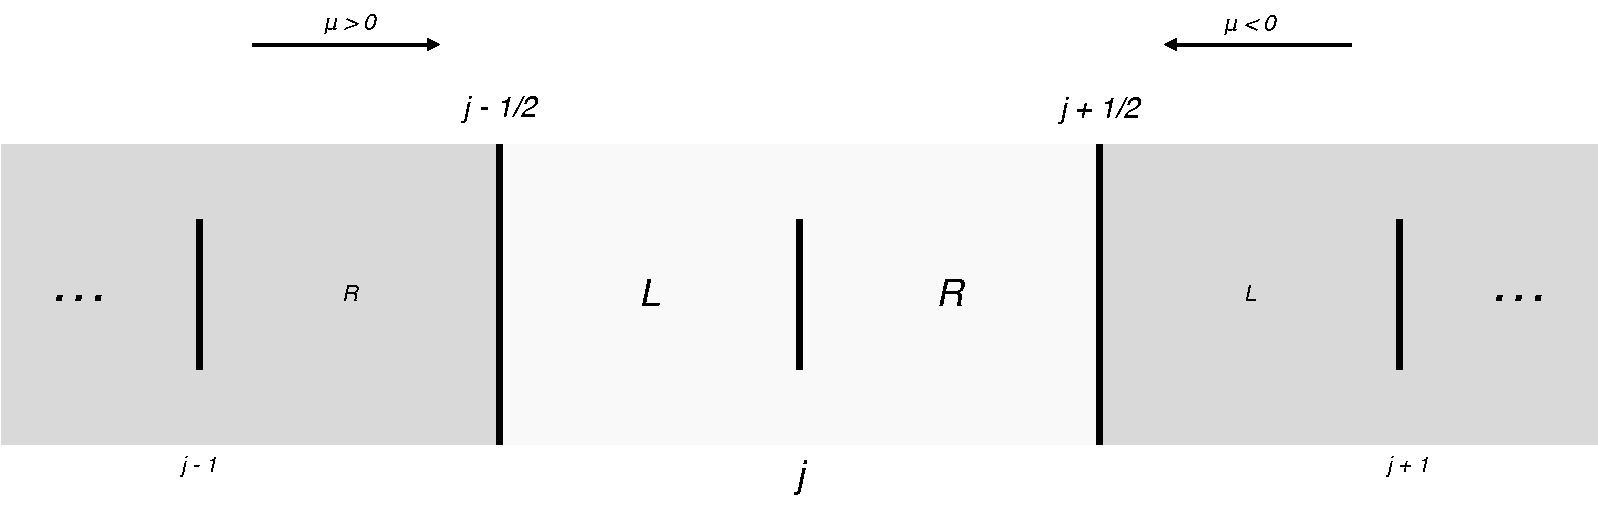
\includegraphics[width=\linewidth]{figures/smm_paper/diag.pdf}
    \caption{Discritization scheme indices; simple corner balance in slab geometry.}
    \label{fig:disc}
\end{figure}

Simple corner balance is a finite element method so the standard Larsen 4-step procedure may produce an inconsistent system of equations which can be algebraically complex to solve \cite{adams_fast_2002}.
In this work we use the modified Adams-Martin 4-step procedure \cite{adams_1992_dsadfe} to derive a set of second moment equations.
The modified four step procedure starts by:

\textit{first} take the 0$^{th}$ angular moments of equations \eqref{eq:scb}:
\begin{subequations}
\label{eq:zeroth}
\begin{equation}
\label{eq:zeroth_left}
    \left[ \frac{J_{j,L} + J_{j.R}}{2} - J_{j-1/2} \right] + \Sigma_{a,j} \frac{\Delta x_j}{2} \phi_{j,L} = \frac{\Delta x_j}{2} \frac{Q_{j,L}}{2} \; ,
\end{equation}
\begin{equation}
     \left[ J_{j+1/2} - \frac{J_{j,L} + J_{j,R}}{2} \right] + \Sigma_{a,j} \frac{\Delta x_j}{2} \phi_{j,R} = \frac{\Delta x_j}{2} \frac{Q_{j,R}}{2} \; ,
\end{equation}
\end{subequations}
where $J$ is the total current (first angular moment). The upstream closure on the right cell edge is
\begin{subequations}
\label{edgescalar}
\begin{equation}
   \phi_{j+1/2} = \sum\limits_{\mu_{m}>0} w_m   \psi_{m,j,R}+\sum\limits_{\mu_{m}<0} w_m \psi_{m,j+1,L} \;,
\end{equation}
and the left is
\begin{equation}
   \phi_{j-1/2} = \sum\limits_{\mu_{m}>0} w_m   \psi_{m,j-1,R}+\sum\limits_{\mu_{m}<0} w_m \psi_{m,j,L} \;,
\end{equation}
\end{subequations}

\textit{Second}: take the 1$^{st}$ angular moments of equations \eqref{eq:zeroth}:
\begin{subequations}
\label{eq:first}
\begin{equation}
    \frac{1}{3} \left[ \frac{\phi_{j,L} + \phi_{j.R}}{2} - \phi_{j-1/2} \right] + \frac{2}{3} \left[ \frac{\Gamma_{j,L} + \Gamma_{j.R}}{2} - \Gamma_{j-1/2} \right] + \Sigma_{t,j} \frac{\Delta x_j}{2} J_{j,L} = 0 \;,
\end{equation}
\begin{equation}
    \frac{1}{3} \left[ \phi_{j+1/2} - \frac{\phi_{j,L} + \phi_{j,R}}{2} \right] +\frac{2}{3} \left[ \Gamma_{j+1/2} - \frac{\Gamma_{j,L} + \Gamma_{j,R}}{2} \right] + \Sigma_{t,j} \frac{\Delta x_j}{2} J_{j,R} = 0 \; ,
\end{equation}
where
\begin{equation}
    \Gamma =  \sum\limits_{m=1}^N w_m   P_2(\mu_m) \psi_{m} = \sum\limits_{m=1}^N w_m \left[ \frac{1}{2} \left( 3 \mu_m^2 - 1 \right) \right]  \psi_{m} \; ,
\end{equation}
\end{subequations}
and is the second angular moment.
The upstream closure on the right cell edge becomes
\begin{subequations}
\label{eq:edgecurrent}
\begin{equation}
   J_{j+1/2} = \sum\limits_{\mu_{m}>0} \mu_m w_m   \psi_{m,j,R}+\sum\limits_{\mu_{m}<0} \mu_m w_m \psi_{m,j+1,L}  \; ,
\end{equation}
and the left cell edge
\begin{equation}
   J_{j-1/2} = \sum\limits_{\mu_{m}>0} \mu_m w_m   \psi_{m,j-1,R}+\sum\limits_{\mu_{m}<0} \mu_m w_m \psi_{m,j,L}  \; .
\end{equation}
\end{subequations}

\textit{Third}, we \textit{modify} Eq. (\ref{edgescalar}) to yield a local expression for the current--one that involves only the scalar fluxes in the cell
\begin{subequations}
\label{eq:modification}
\begin{equation}
    \phi_{j-1/2} = \phi_{j,L} \; ,
\end{equation}
and 
\begin{equation}
    \phi_{j+1/2} = \phi_{j,R} \; ,
\end{equation}
\end{subequations}
then insert into equations into Eqs. \eqref{eq:first}
\begin{subequations}
\label{eq:current}
\begin{equation}
    J_{j,L} = - \frac{1}{3 \Sigma_{t,j} \Delta x_j} \left[ \phi_{j,R} - \phi_{j,L} \right] - \frac{4}{3 \Sigma_{t,j} \Delta x_j} \left[ \frac{\Gamma_{j,L} + \Gamma_{j,R}}{2} - \Gamma_{j-1/2} \right] 
\end{equation}
\begin{equation}
    J_{j,R} = - \frac{1}{3 \Sigma_{t,j} \Delta x_j} \left[ \phi_{j,R} - \phi_{j,L} \right] -\frac{4}{3 \Sigma_{t,j} \Delta x_j} \left[ \Gamma_{j+1/2} - \frac{\Gamma_{j,L} + \Gamma_{j,R}}{2} \right].
\end{equation}
\end{subequations}
We expand the cell edge currents from Eqs. \ref{eq:edgecurrent} using the P$_1$ approximation
\begin{subequations}
\begin{equation}
    J_{j+1/2} = \sum\limits_{\mu_{m}>0} \mu_m w_m   \left(\frac{1}{2} \phi_{j,R} + \frac{3\mu_m}{2} J_{j,R} \right)+\sum\limits_{\mu_{m}<0} \mu_m w_m \left(\frac{1}{2} \phi_{j+1,L} + \frac{3\mu_m}{2} J_{j+1,L} \right)
\end{equation}
and
\begin{equation}
    J_{j-1/2} = \sum\limits_{\mu_{m}>0} \mu_m w_m   \left(\frac{1}{2} \phi_{j-1,R} + \frac{3\mu_m}{2} J_{j-1,R} \right)+\sum\limits_{\mu_{m}<0} \mu_m w_m \left(\frac{1}{2} \phi_{j,L} + \frac{3\mu_m}{2} J_{j,L} \right)
\end{equation}
\end{subequations}
which simplify to
\begin{subequations}
\label{eq:edgecur}
\begin{equation}
    J_{j+1/2} = \gamma \left( \phi_{j,R} - \phi_{j+1,L} \right) + \xi \left( J_{j,R} + J_{j+1,L} \right) \; ,
\end{equation}
and
\begin{equation}
    J_{j-1/2} = \gamma \left( \phi_{j,R-1} - \phi_{j,L} \right) + \xi \left( J_{j-1,R} + J_{j,L} \right) \; ,
\end{equation}
where
\begin{equation}
    \gamma = \frac{1}{2} \sum\limits_{\mu_{m}>0} \mu_m w_m \approx \frac{1}{4} \; ,
\end{equation}
and
\begin{equation}
    \xi = \frac{3}{2} \sum\limits_{\mu_{m}>0} \mu_m^2 w_m \approx \frac{1}{2} \; .
\end{equation}
\end{subequations}

\textit{Fourth} combine Eqs. \eqref{eq:zeroth}, \eqref{eq:current} and \eqref{eq:edgecur} to forum a system of equations
\begin{subequations}
\label{eq:full_secondmomemnt}
\begin{multline}
    -\left(1-\xi \right) D_j \frac{\left( \phi_{j,R} - \phi_{j,L} \right)}{\xi x_j} -\gamma \left( \phi_{j-1,R} - \phi_{j,L} \right) + \xi D_{j-1} \frac{\left( \phi_{j-1,R} - \phi_{j-1,L} \right)}{\Delta x_{j-1}}
    \\
    + \Sigma_{a,j} \frac{\Delta x_j}{2} \phi_{j,L} = \frac{\Delta x_j}{2} \frac{Q_{j,L}}{2} +\frac{2 \xi D_j}{\Delta x_j} \left(\Gamma_{j+1/2} - \Gamma_{j-1/2} \right)
    \\
     - \xi \left[ \frac{4 D_j}{\Delta x_j} \left( \frac{\Gamma_{j,L} + \Gamma_{j,R}}{2} - \Gamma_{j-1/2} \right) + \frac{4 D_{j-1}}{\Delta x_{j-1}} \left(\Gamma_{j-1/2} -  \frac{\Gamma_{j-1,L} + \Gamma_{j-1,R}}{2} \right) \right] \; ,
\end{multline}
and
\begin{multline}
    \left(1-\xi \right) D_j \frac{\left( \phi_{j,R} - \phi_{j,L} \right)}{\Delta x_j} +\gamma \left( \phi_{j,R} - \phi_{j+1,L} \right) - \xi D_{j+1} \frac{\left( \phi_{j+1,R} - \phi_{j+1,L} \right)}{\Delta x_{j+1}}
    \\
    + \Sigma_{a,j} \frac{\Delta x_j}{2} \phi_{j,R} = \frac{\Delta x_j}{2} \frac{Q_{j,R}}{2} -\frac{2 \xi D_j}{\Delta x_j} \left(\Gamma_{j+1/2} - \Gamma_{j-1/2} \right)
    \\
    + \xi \left[ \frac{4 D_j}{\Delta x_j} \left( \Gamma_{j+1/2} - \frac{\Gamma_{j,L} + \Gamma_{j,R}}{2}  \right) + \frac{4 D_{j+1}}{\Delta x_{j+1}} \left( \frac{\Gamma_{j+1,L} + \Gamma_{j+1,R}}{2} - \Gamma_{j+1/2} \right)  \right] \;.
\end{multline}
\end{subequations}

A standard DSA method will discard the second moments and define the source ($Q$) as the error between subsequent iteration (commonly denoted by $\Delta \phi=\phi\la-\phi\lph$).
So the diffusion equations solve for an error estimation scalar flux which can be added to $l+1/2$ quantities to correct them.
In this analysis we Yavuz and Larsen's scheme \cite{yavuz_spatial_1989} and keep the second moments as we solve for physical terms to update $l+1/2$ quantities, \textit{not} an error corrections.
Furthermore we can make a simplification that the second moments incident on the boundary of each cell are,
\begin{subequations}
\label{eq:simple}
\begin{equation}
    \Gamma_{j-1/2} = \Gamma_{j,L}\lph \; ,
\end{equation}
and
\begin{equation}
    \Gamma_{j+1/2} = \Gamma_{j,R}\lph \; ,
\end{equation}
\end{subequations}
so only within cell information is used.
This is similar to the modification the Adams-Martin method makes for the zeroth angular moment in Eqs. \eqref{eq:modification}.
% This simplifies the equations for the within cell currents:
% \begin{equation}
%     J_{j,L} = J_{j,R} = - \frac{1}{3 \Sigma_{t,j} \Delta x_j} \left[ \phi_{j,R} - \phi_{j,L} \right] - \frac{4}{3 \Sigma_{t,j} \Delta x_j} \left[ \Gamma_{j,R} - \Gamma_{j,L}  \right],
% %    \label{fm1}
% \end{equation}
This simplifies Eqs. \eqref{eq:full_secondmomemnt} to be a left side
\begin{subequations}
\label{eq:simple_smom}
\begin{multline}
-\left(1-\xi \right) D_j \frac{\left( \phi_{j,R}^{(l+1)} - \phi_{j,L}^{(l+1)} \right)}{\Delta x_j} -\gamma \left( \phi_{j-1,R}^{(l+1)} - \phi_{j,L}^{(l+1)} \right) + 
\\ 
\xi D_{j-1} \frac{\left( \phi_{j-1,R}^{(l+1)} - \phi_{j-1,L}^{(l+1)} \right)}{\Delta x_{j-1}} 
+ \Sigma_{a,j} \frac{\Delta x_j}{2} \phi_{j,L}^{(l+1)} = \frac{\Delta x_j}{2} \frac{Q_{j,L}}{2} 
\\
+\frac{2D_j( 1- \xi) }{\Delta x_j} \left(\Gamma_{j,R}^{(l+1/2)} - \Gamma_{j,L}^{(l+1/2)} \right) 
- \frac{2 \xi D_{j-1}}{\Delta x_{j-1}} \left( \Gamma_{j-1,R}^{(l+1/2)} - \Gamma_{j-1,L}^{(l+1/2)} \right) \; ,
\end{multline}
and right side
\begin{multline}
\left(1-\xi \right) D_j \frac{\left( \phi_{j,R}^{(l+1)} - \phi_{j,L}^{(l+1)}  \right)}{\Delta x_j} +\gamma \left( \phi_{j,R}^{(l+1)}  - \phi_{j+1,L}^{(l+1)}  \right) - \xi D_{j+1} \frac{\left( \phi_{j+1,R}^{(l+1)}  - \phi_{j+1,L}^{(l+1)}  \right)}{\Delta x_{j+1}} \\
+ \Sigma_{a,j} \frac{\Delta x_j}{2} \phi_{j,R}^{(l+1)}  = \frac{\Delta x_j}{2} \frac{Q_{j,R}}{2} \\
-\frac{2 D_j(\xi-1)}{\Delta x_j} \left(\Gamma_{j,R}^{(l+1/2)} - \Gamma_{j,L}^{(l+1/2)} \right) + \frac{2 \xi D_{j+1}}{\Delta x_{j+1}} \left(\Gamma_{j+1,R}^{(l+1/2)} - \Gamma_{j+1,L}^{(l+1/2)}\right)  \; ,
\end{multline}
\end{subequations}
balance which are written for a mid-step update to scalar flux and use only information coming from within a cell from the high-order transport soultion.
Substituting \eqref{eq:simple} into \eqref{eq:current} forums the updated half-cell volume integrated currents 
\begin{equation}
\label{eq:simp_current}
    J_{j,L}^{(l+1)} = J_{j,R}^{(l+1)} = - \frac{1}{3 \Sigma_{t,j} \Delta x_j} \left[ \phi_{j,R}^{(l+1)} - \phi_{j,L}^{(l+1)} \right] - \frac{4}{3 \Sigma_{t,j} \Delta x_j} \left[ \Gamma_{j,R}^{(l+1/2)} - \Gamma_{j,L}^{(l+1/2)}  \right] \;.
%    \label{fm1}
\end{equation}


\subsection{Boundary Conditions}

Boundary conditions on the left sides (assuming incident angular flux at $x=0$) \eqref{eq:zeroth_left} in the first cell ($j=1$), we find:
\begin{equation}
 \left[ \frac{J_{1,L} + J_{1,R}}{2} - J_{1/2} \right] + \Sigma_{a,1} \frac{\Delta x_1}{2} \phi_{1,L} = \frac{\Delta x_1}{2} \frac{Q_{1,L}}{2}. 
\end{equation}
On the left edge, the current ($J_{1/2}$) is a combination of the incident partial current, which is computed from the known incoming angular flux, and the outgoing partial current, which is computed using the P$_1$ expansion of the angular flux $\psi_{m,1,L}$:
\begin{equation}
    J_{1/2}= J^{-}_{left} - \left(\gamma \phi_{1,L} - \xi J_{1,L}\right) \; ,
\end{equation}
where $J^{-}_{left}$ is the physical boundary condition imposed at the left boundary $j=1/2$
Using the definition of $J_{1,L}$ from Eq. \eqref{eq:simp_current}, we find the first in our systems is
\begin{subequations}
\label{eq:bc_inc}
\begin{multline}
    -\left(1-\xi \right) D_1 \frac{\left( \phi_{1,R} - \phi_{1,L} \right)}{\Delta x_1} +\gamma  \phi_{1,L}  + \Sigma_{a,1} \frac{\Delta x_1}{2} \phi_{1,L} 
    \\ = 
    \frac{\Delta x_1}{2} \frac{Q_{1,L}}{2} +J^{-}_{left}+ 
    \frac{2D}{\Delta x}(\Gamma_{1,R}-\Gamma_{1,L}) \; .
\end{multline}
Likewise for the right ($j=I$) 
\begin{multline}
    \left(1-\xi \right) D_I \frac{\left( \phi_{I,R} - \phi_{I,L} \right)}{\Delta x_I} +\gamma \left( \phi_{I,R}   \right)
    + \Sigma_{a,I} \frac{\Delta x_I}{2} \phi_{I,R}\\ = 
    \frac{\Delta x_I}{2}\frac{Q_I}{2} + J_{right}^+ - \frac{2 D_I}{\Delta x} \left( \Gamma_{I,R} - \Gamma_{I,L}\right)
\end{multline}
\end{subequations}
and is the final equation in the second moment system.

Similarly we can define reflecting (Neumann) boundary conditions at $x=0$, $J_{1/2} = 0$, and this naturally is incorporated into the balance equation for the left-half of cell $j=1$.
Eq. \eqref{eq:zeroth_left} in the first cell ($j=1$), then becomes
\begin{equation}
 \left[ \frac{J_{1,L} + J_{1,R}}{2} \right] + \sigma_{a,1} \frac{\Delta x_1}{2} \phi_{1,L} = \frac{\Delta x_1}{2} \frac{Q_{1,L}}{2}. 
\end{equation}
Inserting the definitions of $J_{1,L}$ and $J_{1,R}$ from Eq. \eqref{eq:simp_current} yields
\begin{subequations}
\begin{equation}
    - D_1 \frac{\left( \phi_{1,R} - \phi_{1,L} \right)}{\Delta x_1}  + \Sigma_{a,1} \frac{\Delta x_1}{2} \phi_{1,L} = \frac{\Delta x_1}{2} \frac{Q_{1,L}}{2} + 
    \frac{2D_1}{\Delta x}(\Gamma_{1,R}-\Gamma_{1,L}) \; .
\end{equation}
Similarly for the right hand side of cell $j+I$ (the right hand side boundary condition)
\begin{equation}
    D_I \frac{\left( \phi_{I,R} - \phi_{I,L} \right)}{\Delta x_I}  + \Sigma_{a,I} \frac{\Delta x_I}{2} \phi_{I,R} = \frac{\Delta x_I}{2} \frac{Q_{I,R}}{2} + 
    \frac{2D_I}{\Delta x}(\Gamma_{I,R}-\Gamma_{I,L}) \; .
\end{equation}
\end{subequations}

\subsection{Cell-wise Updates}

The preceding sections have described a system updating scalar flux and current.
Unlike SI which iterates on, scalar flux OCI iterates exclusively on the angular flux.
Implementations of OCI algorithms may never form the scalar flux while iterating.
This is what makes finding a low-order transport approximation to aid in converging a higher order OCI solve so difficult.
Normal acceleration methods only provide updates for \textit{moments} of angular flux in the sourcing side of the equation for the next iteration.


The domain decomposition method in \cite{yavuz_spatial_1989} describe a remainder on the surfaces of the boundary conditions.
Finally we update all incident angular fluxes on the surface of the cell with
\begin{equation}
    \label{eq:update}
    \af\lp_{m,j,L/R} = \af_{m,j,L/R}\lph + \frac{1}{2}\left[\left(\phi_{j,R/L}\lp - \phi_{j,R/L}\lph\right) + 3\mu_m\left(J_{j,L/R}\lp - J_{j,L/R}\lph\right)\right] \;.
\end{equation}
This update removes the zeroth and first order moments from the $l+1/2$ angular flux and replaces them with zeroth and first order moments from the solution of the second moment equations to produce a new incident angular flux on all cell bounds for $l+1$.
Notably the second moment equations where driven by material properties and information from the high-order transport solution at $l+1/2$.
This solution is also commuted globally.

Once update for all incident angular flux is found on all cells the algorithm can continue until
\begin{subequations}
\begin{equation}
\label{eq:convergence_crit}
    ||\psi^{(l+1)}-\psi^{(l)}|_{2} < \epsilon(1-\rho_{e}) \; ,
\end{equation}
controlling for false convergence when spectral radius is near unity, where $\epsilon$ is the convergence tolerance and
\begin{equation}
\label{eq:spec_rad_est}
    \rho_{e} = \frac{||{\psi}^{(l+1)}-{\psi}^{(l)}||_{2}}{||{\psi}^{(l)}-{\psi}^{(l-1)}||_{2}} \; ,
\end{equation}
\end{subequations}
is an empirical estimation of the spectral radius computed at every iteration of a transport solve. 


\begin{algorithm}
\begin{algorithmic}[1]

    \State initial guess for $\psi$

    \While{not converged}

        \State $\psi\lph =$ OCI iteration using $\psi\la$

        \State compute half-cell volume $\phi\lph$, $J\lph$, and $\Gamma\lph$ from $\psi\lph$

        \State solve second moment equations for $\phi\lp$ \Comment{Eq. \eqref{eq:simple_smom}}

        \State solve for updated currents $J\lp$ \Comment{Eq. \eqref{eq:simp_current}}

        \State compute new angular fluxes using the Yavuz update \Comment{Eq. \eqref{eq:update}}

        \State $e\lph=|\psi\lph - \psi\la|_2$

        \State $\rho_e = e\lph / e\la$ \Comment{Eq. \eqref{eq:spec_rad_est}}

        \If{$e < \epsilon(1-\rho_e)$} \Comment{Eq. \eqref{eq:convergence_crit}}
            \State converged = true
        \Else 

            \State $e\la = e\lph$
    
            \State $\psi\la = \psi\lp$ 
        \EndIf
    \EndWhile
    
    \caption{A One cell inversion iteration with second moment method updating incident angular fluxes on the surface of every cell. Constructed so only a transport solution is used to measure error and test convergence.}
    \label{alg:smmoci}
\end{algorithmic}
\end{algorithm}


Algorithm \ref{alg:smmoci} shows how this second moment method would be implemented with an OCI solve.
The OCI iteration is parallel over all angle and the block tri-diagonal diffusion matrix may be solved using any number of libraries optimized for execution on both CPU and GPU (e.g., cu/rocSPARSE \cite{cusparse, rocsparse}, MAGMA \cite{magma}, or others \cite{liwen_2012_solveable, klein_2023_tridiag}).
It has previously been shown that OCI algorithms lend themselves to implementation with linear algebra libraries which in-turn enables performance portability and more rapid methods development \cite{morgan_2025_oci}.
The second moment algorithm shown in \ref{alg:smmoci} does not change that.


\section{Verification}

To verify that this method is providing expected solutions we use many anaclitic and benchmark problems with reference solutions.
We start by verifying the diffusion equations (setting second moments to zero) and verify using the method of manufactured solutions.
We compare the solutions computed by OCI and the second moment method to (1) a source free homogeneous slab (referenced to an SI solver), a 3 region purely absorbing slab (referenced to an anaclitic solution) and a multi-region highly scattering slab (referenced to highly resolved Monte Carlo result). 

Before confirming the full preconditioning scheme described in section \ref{sec:methods} we use the method of manufactured solutions to verify the low-order diffusion equations produce the expected result \cite{warsa_mms_2010, moosemms}.
The diffusion equations for SCB are Equations \ref{eq:full_secondmomemnt} with the contribution of the second moments was neglected (as would be the case for traditional DSA).
Figure \ref{fig:diffusion_mms} shows the solution to a linear and quadratic manufactured solution on the left and right respectively.
To solve for a \textit{manufactured} source ($Q^m$) a \textit{manufactured} solution ($\phi^m$) can be produced with any and supplied to the continuous, one-speed, steady state, neutron diffusion equation
\begin{equation}
    -\frac{1}{3\Sigma}\frac{d^2\phi^m(x)}{dx^2} - \Sigma_a\phi(x)  = Q^m(x) \;.
\end{equation}
We then use $Q^m$ to produce half-cell volume integrated material sources over the problem domain ($x=[0,4]$\unit{\centi\meter}) with $\Sigma =$ \SI{10.0}{\per\centi\meter}, $\Sigma_s =$ \SI{5.0}{\per\centi\meter}, and $\Delta x =$ \SI{0.1}{\per\centi\meter}.
Figure \ref{fig:diffusion_mms} shows the diffusion equation matching the manufactured solution for both manufactured solutions considered including into nonphysical negative source.
This demonstrates that the low-order diffusion equations are robust to nonphysical negative values.

\begin{figure}
    \centering
    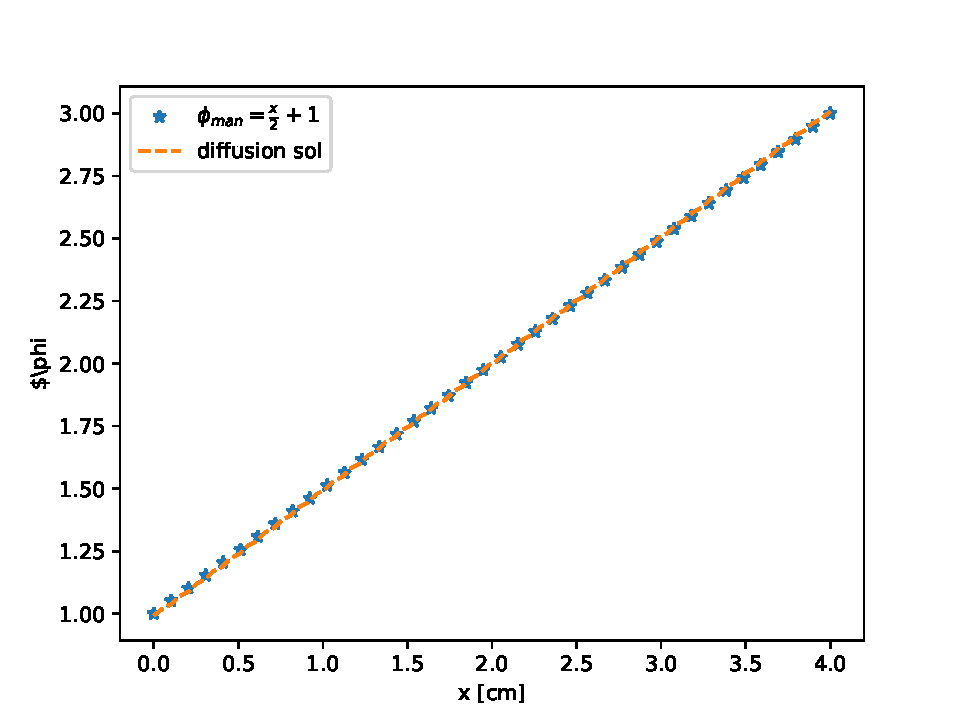
\includegraphics[width=.49\linewidth]{figures/smm_paper/linear_mms.pdf}
    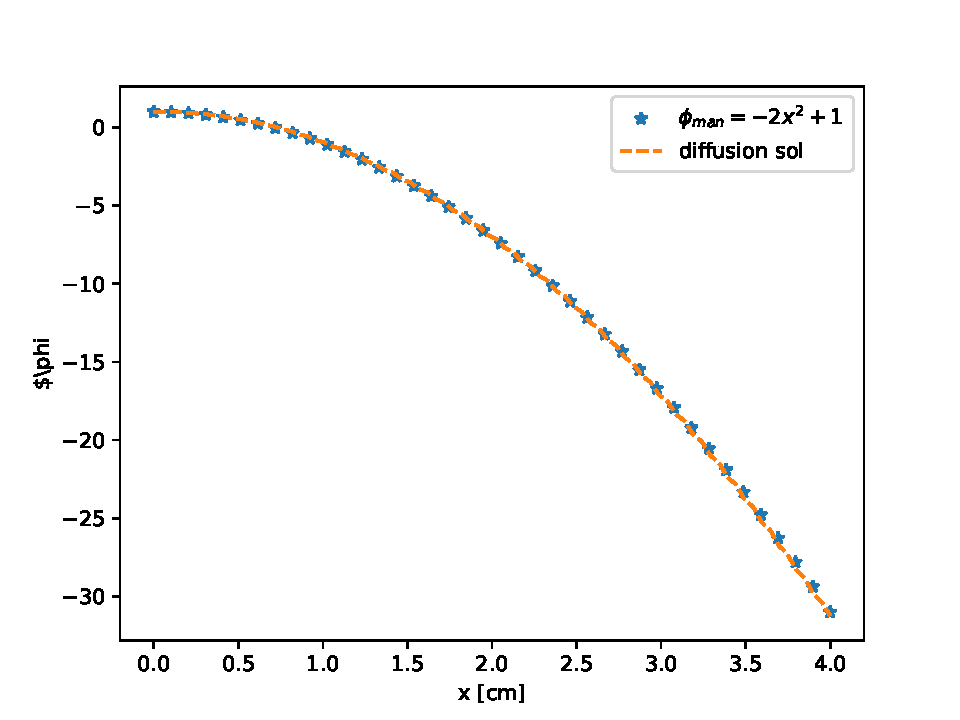
\includegraphics[width=.49\linewidth]{figures/smm_paper/quadratic_mms.pdf}
    \caption{Verification of the low-order diffusion equations using quadratic and linear manufactured solutions}
    \label{fig:diffusion_mms}
\end{figure}

To verify that our full second moment preconditioner produces the correct transport solutions we used a number of 1D benchmark problems.
We started with canonical transport problems including the infinite-homogeneous medium problem (using both reflecting and incident angular flux prescriptions) and the source free pure absorber.
Both iterative methods converged to the expected analytical solutions for these problems.

Next we consider three slab problems with increasing complexity.
First we use a \SI{4}{\centi\meter} wide source free homogeneous slab where $\Sigma=$ \SI{1.0}{\per\centi\meter}, $\Sigma_s=$ \SI{0.5}{\per\centi\meter}, with an incident angular flux on the left of $\psi_{left}^-=$ \SI{5}{\per\centi\meter\cubed\per\s} and vacuum on the right.
In all work in this paper we use a convergence criterion of $\epsilon = $ \num{1e-5} and maximum iteration count of \num{1e4}.
We compare the the solution from OCI and the second movement method to one generated from a source iteration solver using lumped-linear discontinuous finite element method.
In 1D, lumped-linear discontinuous is equivalent to the simple corner balance method we implement in this work \cite{adams_subcell_1997}.
Figure \ref{fig:regression_slab} compares the solution in both S$_2$ and S$_4$ showing a slight deviation between the two transport results and the second moment solution.
The number of iterations is shown in the legend of either plot.
In S$_2$ OCI takes 212 iterations whereas the second moment method converges instantly (the solver forces at least 3).
We found that for all problems considered in S$_2$, the second moment method will converge after a single iteration.
This is because the DSA equations are themselves the P$_1$ equations which are equivariant to S$_2$ in 1D slab geometry.
In S$_4$ convergence is achieved after \num{197} and \num{127} for OCI and the second moment method respectively.

\begin{figure}
    \centering
    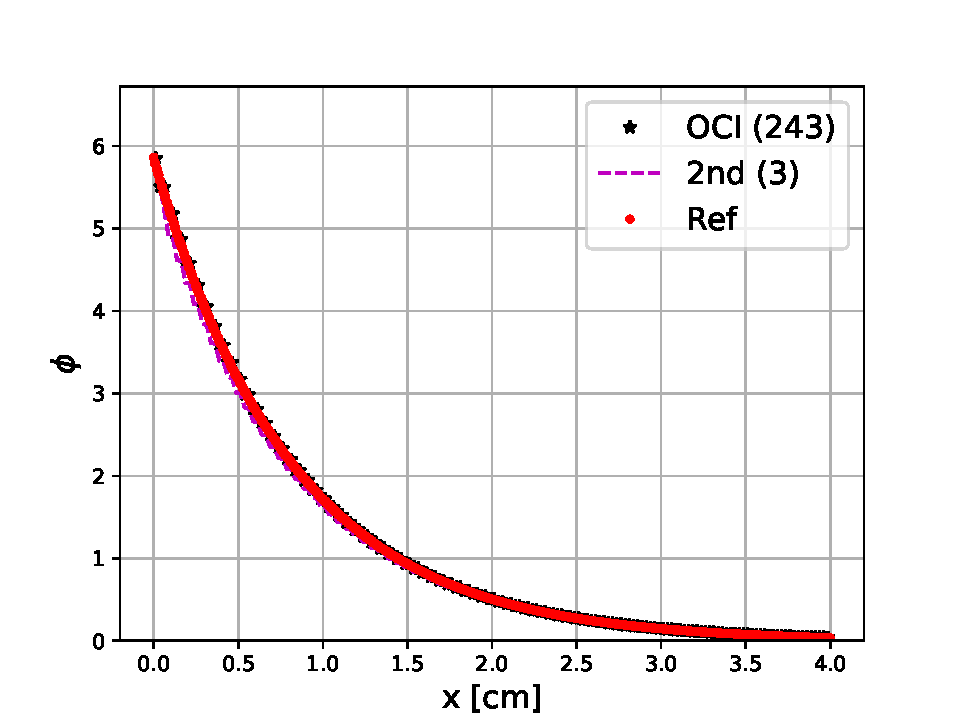
\includegraphics[width=.49\linewidth]{figures/smm_paper/regression_slabs2.pdf}
    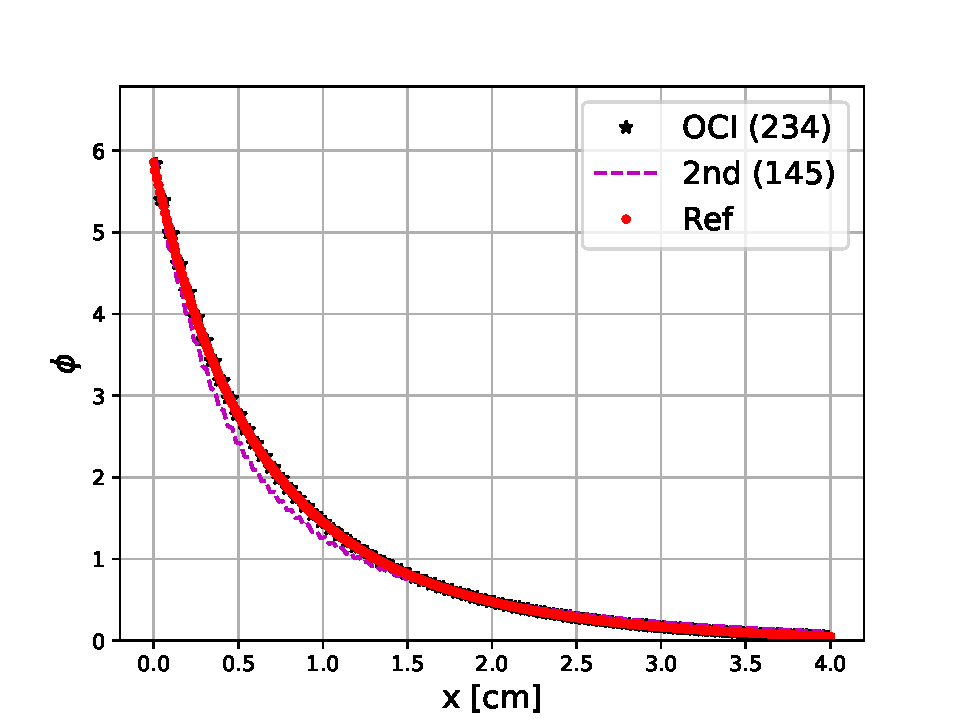
\includegraphics[width=.49\linewidth]{figures/smm_paper/regression_slabs4.pdf}
    \caption{Solution to a source free slab the solution between OCI, the second moment method and a solution from a lumped linear discontinuous source iteration solver in S$_2$ (left) and S$_4$ (right).}
    \label{fig:regression_slab}
\end{figure}
 
Figure \ref{fig:absorbium} shows the solution for a three region purely absorbing slab where $\Sigma = $ \qtylist{1.5; 2.0; 1.0}{\per\centi\meter} for region 1 (\SI{0}{\centi\meter}--\SI{2}{\centi\meter}), 2 (\SI{2}{\centi\meter}--\SI{4}{\centi\meter}) and 3 (\SI{4}{\centi\meter}--\SI{6}{\centi\meter}), respectively.
There is an isotropic material source distributed thorough out the whole problem domain ($Q=$ \SI{1.0}{\per\centi\meter\cubed\per\s}) vacuum boundary conditions on the left and right and we use $\Delta x = $\SI{0.05}{\centi\meter} in S$_{16}$.
Figure \ref{fig:absorbium} at left shows $\phi$ for both OCI and the second moment method as well as the solution from a closed forum anaclitic function.

The scalar fluxes match to within three decimal places suggesting a matching solution.
However, figure  \ref{fig:absorbium} at right also shows angular flux as a function of both space and angle.
The transport solution seems to match the reference solution clearly, however the second moment method smears contribution.
This may be from the assumed isotropy that is enforced at all cell incident cell interfaces. 
Notably this solution was archived in the same number of iterations for either method (\num{121}) suggesting the second moment method provides no aid to $\rho$ without scattering.

\begin{figure}
    \centering
    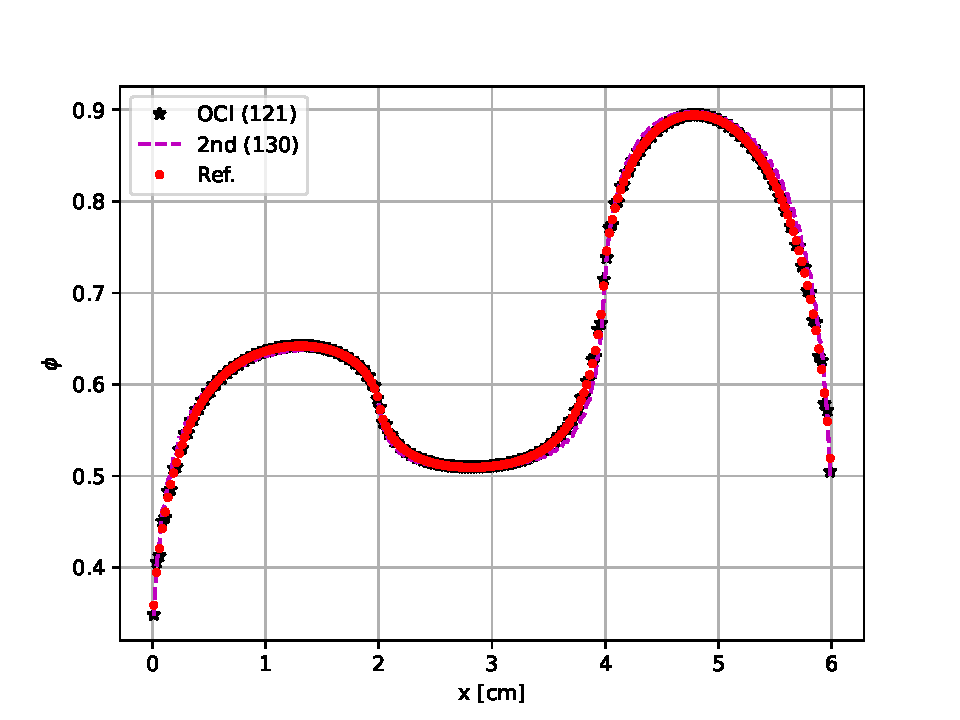
\includegraphics[width=.49\linewidth]{figures/smm_paper/slab_abs_sf.pdf}
    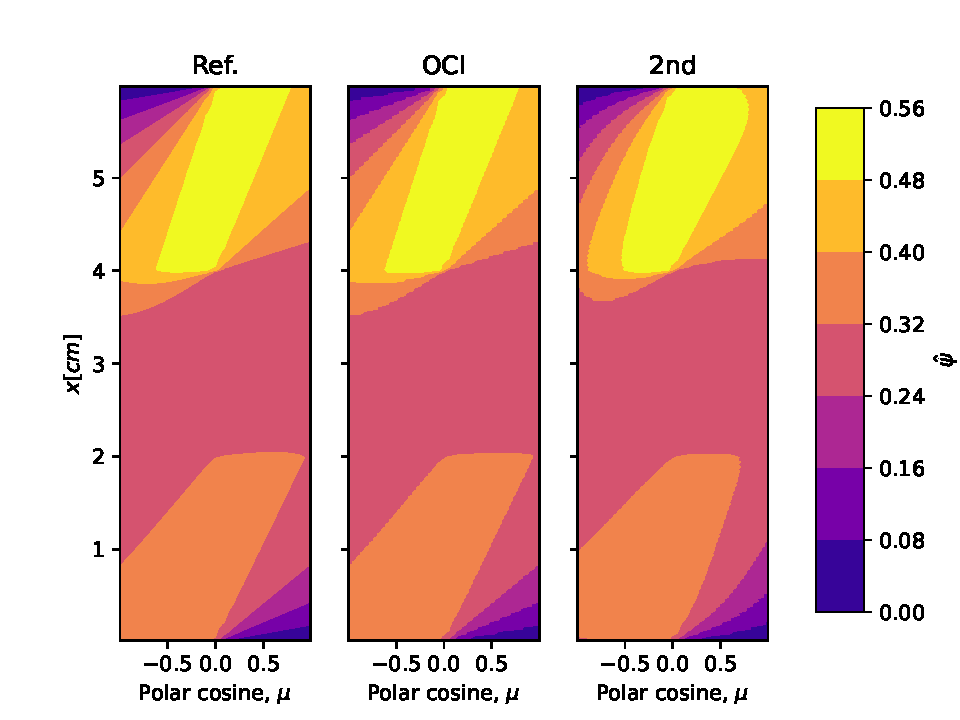
\includegraphics[width=.49\linewidth]{figures/smm_paper/slab_abs_af.pdf}
    \caption{Solution to the three-region purely absorbing slab problem with an anaclitic reference solution for $\phi$ (left) and $\psi$ (right) in S$_{16}$ with $\Delta x =$\SI{0.05}{\centi\meter}}
    \label{fig:absorbium}
\end{figure}

Finally we consider a problem described by Yavuz and Larsen shown in table \ref{tab:yavuz_problem} \cite{yavuz_spatial_1989}.
We solve this problem in the thin limit (using $\Delta x=$ \SI{0.01}{\centi\meter}) with a high quadrature order (S$_{31}$) and make comparisons to a Monte Carlo solution provided from MC/DC \cite{morgan_monte_2024}.
The Monte Carlo solution uses 100 evenly spaced tally bins in $x$ and 32 tally bins polar angle, between $[-1, 1]$.
We ran this solution with \num{1e9} particles ran across 10 batches.
The total variance from this solution is \num{1.41e-3}.

\begin{table}
    \centering
    \begin{tabular}{cccc}
        \hline
        Region & Q \unit{\per\centi\meter\cubed\per\s} & $\Sigma$ \unit{\per\centi\meter} & $\Sigma_s$ \unit{\per\centi\meter}  \\
        \hline
        1 (\SI{0}{\centi\meter}--\SI{1}{\centi\meter}) & \num{0.0} & \num{1.0} & \num{1.00}\\
        2 (\SI{1}{\centi\meter}--\SI{2}{\centi\meter}) & \num{1.0} & \num{1.0} & \num{0.95}\\
        3 (\SI{2}{\centi\meter}--\SI{3}{\centi\meter}) & \num{1.0} & \num{1.0} & \num{0.80}\\
        4 (\SI{3}{\centi\meter}--\SI{4}{\centi\meter}) & \num{0.0} & \num{1.0} & \num{0.95}\\
        \hline
    \end{tabular}
    \caption{Yavuz 4-region highly scattering slab problem \cite{yavuz_spatial_1989}.}
    \label{tab:yavuz_problem}
\end{table}

Figure \ref{fig:yavuz} shows the results for ($\phi$ at left and $\psi$ ar right) again between OCI, the second moment method, and the reference Monte Carlo solution.
Note that all these solutions are normalized to compare to a Monte Carlo result which only provide shape solutions.
OCI matches the Monte Carlo solution.
The second moment method again appears to deviate significantly starting in the lowest scattering region (region 3).
This the spatially converged solution that does not noticeably change as $\Delta x \rightarrow 0$.
The angular flux appears smeared again suggesting an impact from low-order cell wise updates.
One thing to note is that OCI converges this problem in \num{3209} iterations where the second moment method takes only \num{765}, a 4.2$\times$ reduction.

\begin{figure}
    \centering
    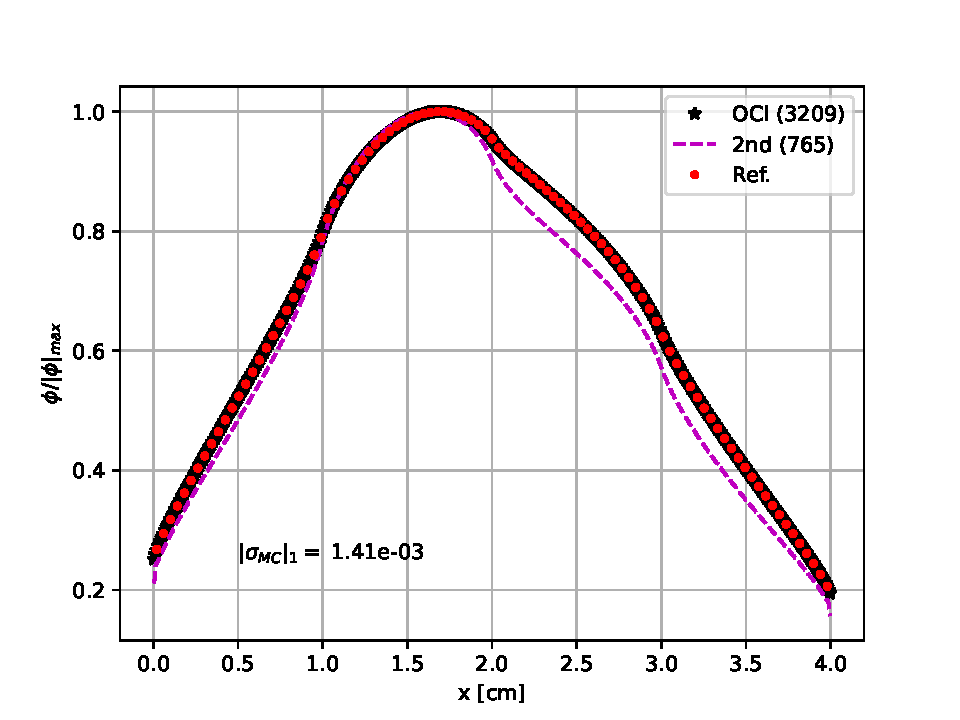
\includegraphics[width=.49\linewidth]{figures/smm_paper/yavuz_normalized_fluxes.pdf}
    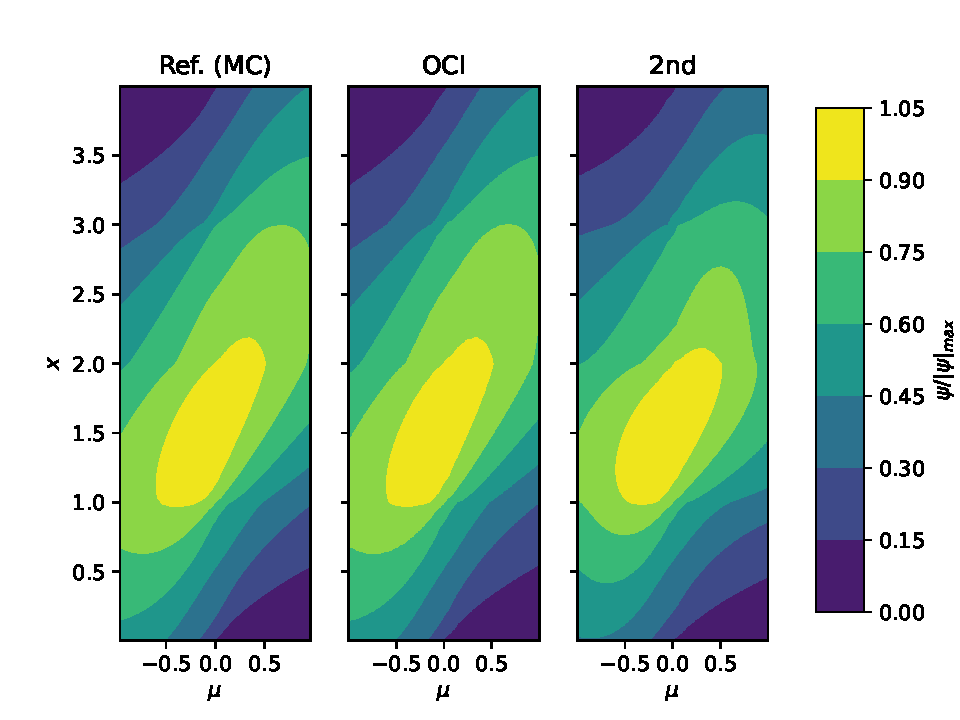
\includegraphics[width=.49\linewidth]{figures/smm_paper/yavuz_af.pdf}
    \caption{Solution to the Yavuz problem via OCI, second moment method, and Monte Carlo results for $\phi$ (left) and $\psi$ (right) in S$_{32}$ with $\Delta x =$\SI{0.01}{\centi\meter}. All solutions have been normalized to compare to Monte Carlo results.}
    \label{fig:yavuz}
\end{figure}


\section{Numerical Experiment}

To demonstrate the convergence behavior of the second moment method across parameter space ($\delta \in [.01,10]$ and $c \in [0,1.0]$) we conduct a numerical experiment of a \SI{25}{\centi\meter} thick source-free infinite homogeneous slab with vacuum boundary conditions in S$_8$.
We hold all other parameters constant and vary $\delta$ and $c$ by varying $\Delta x$ and $\Sigma_s$ respectively.
For both algorithms we initialize the iteration randomly with $\psi^{0} \in [0, 1]$ to excite all error modes and measure error via the anaclitic (trivial solution)
\begin{equation}
    e = ||\psi^l - \bm{0}||_2 \;.
\end{equation}
Spectral radius is then empirically measured with equation \ref{eq:spec_rad_est}.

\begin{figure}
    \centering
    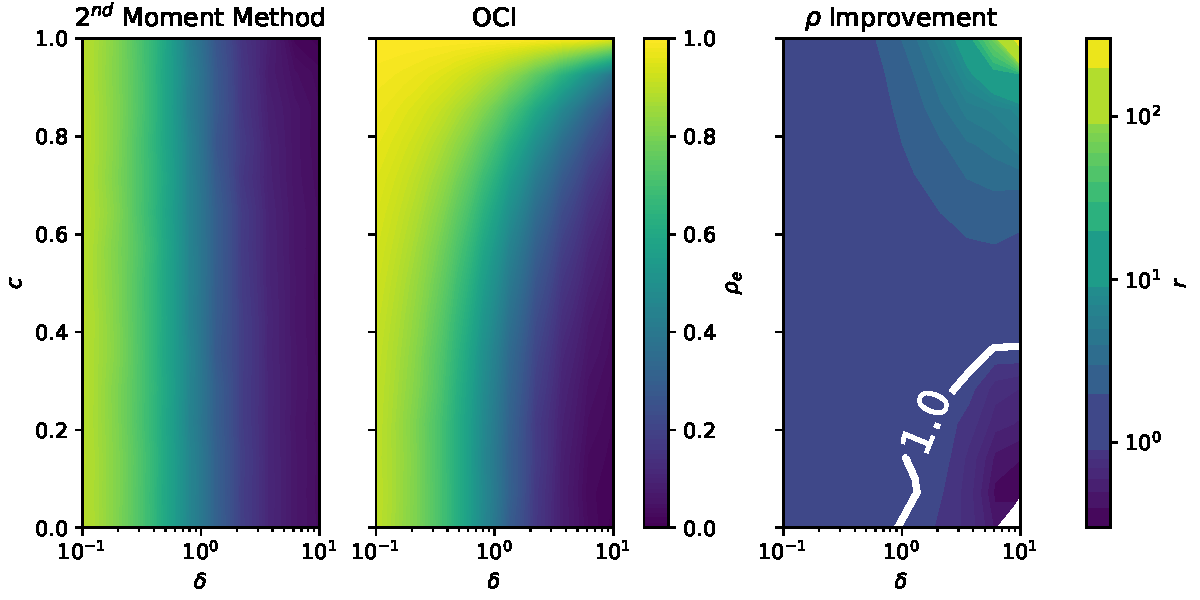
\includegraphics[width=\linewidth]{figures/smm_paper/smm_acc.pdf}
    \caption{Empirical estimations of spectral radius ($\rho$) over choices of perameter space for the second moment method (left) and OCI (middle) from an infinite homogeneous medium problem in S$_8$ where $\psi^{0} \in [0,1]$. The ratio of $\rho_{OCI} / \rho_{SMoM}$ (right), log color scale.}
    \label{fig:spec_rad}
\end{figure}

Figure \ref{fig:spec_rad} shows empirical measurements of spectral radius for the second moment method (left) and OCI (middle) as functions of mean free path ($\delta$) and scattering ratio ($c$).
The measured spectral radius for OCI is the same as the solution provided via Fourier analysis in Figure \ref{fig:ss_spec_rads}.
The maximum spectral radius measured for OCI is \num{1.0} (OCI did not converge in the maximum iteration count) where the second moment is only \num{0.89}, potentially the difference of thousands of iterations.

Figure \ref{fig:spec_rad} at left shows the second moment method effectively eliminating convergence issues in the diffusive limit making $\rho$ entirely a function of cellular optical thickness ($\delta$).
As expected it does not seem to aid convergence in the thin limit.

Figure \ref{fig:spec_rad} at right shows
\begin{equation}
    r = \frac{\rho_{OCI}}{\rho_{SMM}} \; ,
\end{equation}
where $\rho_{OCI}$ and $\rho_{SMM}$ are the empirically measured spectral radii OCI and the second moment method respectively.
This shows the region where the second moment method benefits convergence rate.
Everything to the left and above the line is where $r > 1$, indicating the second moment method is providing an improvement to spectral properties.
The most significant improvement is in the thick diffusive limit (upper right hand corner) which sees maximum 248$\times$ improvement in the parameter range we considered.
Marginal improvement is shown in most other regions---ratios between $1.0\times$ and $2.0\times$.
Decreased convergence rate is shown in the thick-streaming limit (lower right hand corner) where unpreconditioned OCI has exceptional convergence behavior.

\section{Discussion, Conclusions, and Future Work}

We use a second moment cellular decomposition method described by Larsen and Yavuz \cite{yavuz_spatial_1989} in conjunction with a one-cell inversion iterations \cite{rosa_cellwise_2013, morgan_2025_oci} in an effort to produce a fully space parallel, rapidly convergent, transport iteration.
We derived and implemented the second moment equations with OCI and a simple corner balance space discritization scheme.
A number of verification problems showed that the converged solution provided by the second moment equations can deviate from the expected transport and reference solutions.
We believe this is due to the simple within cell closures in Equations \label{eq:simple_close}.
When the full second moment equations are implemented we do not expect the convergence behavior shown in Figure \ref{fig:spec_rad} to change significantly as it aligns with previous results when this method was used as a domain decomposition method in conjunction to SI \cite{yavuz_spatial_1989}.

In S$_2$ the second moment scheme will converge after a single iteration.
This is because the DSA equations are themselves the P$_1$ expansions of the transport solution which are in-turn equivariant to the S$_2$ equations in 1D.
The second moment method seems to eliminate any dependence of the spectral radius ($\rho$) on scattering ratio ($c$) making it entirely a function of cellular optical thickness ($\delta$).
For optically thick this method is rapidly convergent regardless of scattering ratio.

For optically thick problems this second moment method does not seem to aid convergence.
This aggress with previous work: Yavuz and Larsen state in their paper ``...although there is a degradation in the performance of the new SI and DSA [block Jacobi domain decomposition] algorithms as the size of the spatial subsystems decreases, this degradation is not serious until these subsystems are less than about a mean free path in diameter \cite{yavuz_spatial_1989}." 
However, for optically thin time dependent problems using OCI iterations we have already shown that small mean free times will push the spectral radius to zero \cite{morgan_2025_oci}.
So for highly time-dependent problems in the diffusive limit that demand significant temporal resolution this second moment method may allow for rapidly convergent space-parallel transport iterations, however this has yet to be shown.

We initially investigated a few synthetic acceleration schemes to converge OCI in both the scattering and thin-limits including using a streaming only problem as a low-order synthetic accelerator which can be computed in a space parallel manor.
Fourier analysis for the streaming only problem indicated no acceleration would be provided by error corrections from the low-order problem.
TSA with $\beta=1$  uses a streaming+absorbing problem as a synthetic accelerator but requires a sweep \cite{tsa2009rosa}.

Moving forward we will implement the full second moment equations (without making within cell closures for second moments) in an attempt to reverify the
We also plan to explore a standard DSA approach for solving mid-step updates of the zeroth and first angular moments, then assuming linear-anisotropy use the update in Equation \ref{eq:update}.
We will also investigate the impact non-stationary iteration schemes---namely GMRES.


\section*{Acknowledgments}

This work was supported by the Center for Exascale Monte-Carlo Neutron Transport (CEMeNT) a PSAAP-III project funded by the Department of Energy, grant number: DE-NA003967.



\part{Monte Carlo Transport}
\label{part:mc}




\chapter{Introduction to Monte Carlo Methods}

\label{chap:mc_methods_intro}

%Predicting how neutrons move through space and time is important when modeling inertial confinement fusion systems, pulsed neutron sources, and nuclear criticality safety experiments, among other systems.

While deterministic schemes produce an exact solution to an inexact problem, Monte Carlo methods provide an inexact solution---with an associated error---to an exact problem.
Monte Carlo methods can treat the independent variables of the NTE (space, angle, time, energy) as continuous, thus eliminating the discretization errors seen with deterministic methods.
The behavior of neutrons can be modeled with a Monte Carlo simulation, where pseudo-particles with statistical importance are created and transported to produce a particle history \cite{lewis_computational_1984}.
A particle's path and the specific set of events that occur within its history are governed by pseudo-random numbers, known probabilities (e.g., from material data), and known geometries.
Data about how particles move and/or interact with the system are tallied to solve for parameters of interest with an associated statistical error from the Monte Carlo process. 
The analog Monte Carlo method is slow to converge (with a convergence rate of $\mathcal{O}(1/\sqrt{n})$ where $n$ is the number of simulated particles).
New Monte Carlo schemes could converge the solution faster in wall-clock time with fewer simulated particles and may be needed to effectively simulate some systems.

%history with interesting citations
%Monte Carlo methods where orignal propased by Stanislaw Ulam in 1946 after work on the Manhattan project.
%It's orginal use in fact was the tracking neutrons thru phase space using handheld computers called Fermiacs.
%The challenge problem I seek to investate also dates back this time.
%Since then from a report in 1995 over 60\% of computational time on US Government super computing systems was concerend with converging the Monte Carlo method

% deception of the section
My work with Monte Carlo schemes---as with my deterministic work---is broadly divided into two categories
\begin{enumerate}
    \item How to use software engineering libraries to implement work more efficiently (RQ 1); and
    \item Novel methods to converge the solution faster on modern hardware (RQ 5).
\end{enumerate}
The first section digs into the first goal, examining performance portability schemes in high-level languages and the work that is currently deployed in Monte Carlo/Dynamic Code (MC/DC) as part of my work with the Center for Exascale Monte Carlo Neutron Transport (CEMeNT).
The second contains work initially done in a production code at Los Alamos National Laboratory and a proposed extension of the scheme the scheme in an implementation in MC/DC.

\subsection{Portability frameworks for Monte Carlo methods}

In this section I introduce initial investigations into high-level performance portability frameworks.
Developing software to simulate physical problems that demand HPC is difficult.
Modern HPCs commonly use both CPUs and GPUs from various vendors.
Years can be spent porting a code from CPUs to run on GPUs, then again when moving from one GPU vendor to the next \cite{pozulp_progress_2023}.
Portability issues compound when designing software for rapidly developing numerical methods where algorithms need to be both implemented and tested at scale.
Finding a software engineering approach that balances the need for portability, rapid development, open collaboration, and performance can be challenging especially when numerical schemes do not rely on operations commonly implemented in libraries   (i.e., linear algebra as in LAPACK or Intel MKL). 

Common HPC software engineering requirements are often met using a Python-as-glue-based approach, where peripheral functionality (e.g., MPI calls, I/O) is implemented using Python packages but compiled functions are called through Python's C-interface where performance is needed.
Python-as-glue does not necessarily assist in the production of the compiled compute kernels themselves---what the Python is gluing together---but can go a long way in simplifying the overhead of peripheral requirements of HPC software.
With this technique, environment management and packaging uses \texttt{pip}, \texttt{conda}, or \texttt{spack}, input/output with \texttt{h5py}, MPI calls with \texttt{mpi4py}, 
and automated testing with \texttt{pytest}, which can all ease initial development and continued support for these imperative operations. 

Many tools have been developed to extend the Python-as-glue scheme to allow producing single-source compute kernels for both CPUs and GPUs.
% a DSL, pyfr
One tactic is to use a domain-specific language to avoid needing a low-level language (e.g., FORTRAN, C).
A domain-specific language is designed to alleviate development difficulties for a group of subject-area experts and can abstract hardware targets if defined with that goal.
%It can even abstract hardware targets if it is defined with that goal.
PyFR, for example, is an open-source computational fluid dynamics solver that implements a domain-specific language plus Python structure to run on CPUs and Nvidia, Intel, and AMD GPUs~\cite{pyfrPetascale}. 
%The overhead of this Python glue is less than 1\% in PyFR.
Witherden et al.~\cite{pyfrPetascale} discussed how this scheme allows PyFR developers to rapidly deploy numerical methods at deployment HPC scales and have demonstrated performance at the petascale.

Other projects have addressed the need to write user-defined compute kernels entirely in Python script.
Numba is a compiler that lowers a small subset of Python code with NumPy arrays and functions into LLVM, then just in time (JIT) compiles to a specific hardware target \cite{lam_numba_2015}. 
Numba also compiles global and device functions for Nvidia GPUs from compute kernels defined in Python.
API calls are made through Numba on both the Python side (e.g., allocate and move data to and from the GPU) and within compiled device functions (e.g., to execute atomic operations).
When compiling to GPUs, Numba supports an even smaller subset of Python, losing most of the operability with NumPy functions.
If functions are defined using only that smallest subset, Numba can compile the same functions to CPUs or GPUs, or execute those functions purely in Python.
Numba data allocations on the GPU can be consumed and ingested by functions from CuPy if linear-algebra operations are required in conjunction with user-defined compute kernels.
When targeting use of a Python portability scheme to HPC for neutron transport I compared the same transient Monte Carlo neutron transport algorithm in various implementations using PyKokkos \cite{AlAwarETAL21PyKokkos}, PyCUDA/PyOpenCL \cite{kloeckner_pycuda_2012}, and Numba \cite{morgan2022}.
After these initial investigations a Numba+mpi4py software engineering scheme was deemed the most viable for implementation in MC/DC.

%Numba has been shown to be slower then other high level portability frameworks for unoptimized matrix multiplication \cite{Godoy_2023}.
%Monte Carlo neutronic workflows are so memory bound that it's doubtful even significant changes to FLOP performance of a 


%
%I found that all three methods produced similar runtimes for our workflows on CPUs and GPUs for a simple transient Monte Carlo neutron transport simulation \cite{morgan2022}.
%Ultimately, we decided to use a Numba + mpi4py development scheme to build out a Monte Carlo neutron transport code for rapid numerical methods development, portable to various HPC architectures \cite{variansyah_mc23_mcdc,morgan_monte_2024,transport_cement_mcdc_2024} (RQ 1).

\subsection{Delta tracking}

This section describes a variance reduction technique that propose to implement in MC/DC.
Woodcock, or delta, tracking \cite{woodcock_techniques_1965} is a variance-reduction technique that computes the majorant cross-section for the whole problem space, then uses it to determine a distance to collision for all particles.
Coupled with rejection sampling to sort for phantom collisions, and a collision estimator to compute scalar flux, delta tracking often improves performance over analogue Monte Carlo in problems that warrant it (problems with a long mean free path).
Many production Monte Carlo Neutron transport codes like Serpent \cite{leppanen_development_2013, leppanen_use_2017, leppanen_2010_burnup} and others \cite{delta2017rowland} use this method.
In traditional delta tracking first the macroscopic majorant cross section is computed for the entire problem space
\begin{equation}
    \label{eq:majorant}
    \Sigma_{M}(E) = \max\left(\Sigma_{b}(E), ..., \Sigma_{B}(E)\right) \,\text{,}
\end{equation}
where $E$ is energy, $\Sigma_{M}$ is the microscopic majorant cross-section, and $\Sigma_{b}$ is the total microscopic cross-section of the $=b^{\text{th}}$ material.
Now to sample a the distance to a collision
\begin{equation}
    \label{eq:sample}
    D = \frac{-\ln{\xi}}{\Sigma_{M}(E)} \, \text{,} 
\end{equation}
where $\xi\in[0,1]$.
If the potential collision occurs, we move the particle to the sampled distance and do rejection sampling, since we are now potentially forcing collisions that did not occur.
We sort out these phantom collisions by allowing particles to continue to a new sampled distance if
\begin{equation}
    \label{eq:reject}
    \xi < \frac{ \Sigma_{j}(E) } { \Sigma_M(E) } \, \text{,}
\end{equation}
where $\xi\in[0,1]$ is a new random number and $\Sigma_{j}(E)$ is the total macroscopic cross-section of the material ($j^{th}$) where the particle currently resides.
Standard delta tracking is required to use a collision estimator which is less efficient then the normal track length estimator used in surface tracking~\cite{mc2018}.
My goal is to find a way to use the track-length estimator while doing delta tracking which may improve the performance of a Monte Carlo code (RQ 5).


\section{Summary of Part and relation to research questions}


Chapter \ref{chap:joss_paper}
We designed Monte Carlo / Dynamic Code (MC/DC) to explore such novel numerical methods on modern high-performance computing systems.
We avoid the need for a compiled or domain-specific language by using the Numba compiler for Python to accelerate and abstract our compute kernels to near compiled code speeds.
We have implemented novel algorithms using this scheme and, in some verification tests, have approached the performance of industry-standard codes at the scale of tens of thousands of processors.

Chapter \ref{chap:cise_paper} Finding a software engineering approach that allows for portability, rapid development, and open collaboration for high-performance computing on GPUs and CPUs is a challenge. 
We implement a portability scheme using the Numba compiler for Python in Monte Carlo / Dynamic Code (MC/DC), a new neutron transport application for rapidly developing Monte Carlo. 
Using this scheme, we have built MC/DC as an application that can run as a pure Python, compiled CPU, or compiled GPU solver. 
In GPU mode, we use Numba paired with an asynchronous GPU scheduler called Harmonize to increase GPU performance. We present performance results (including weak scaling up to 256 nodes) for a time-dependent problem on both CPUs and GPUs and compare favorably to a production C++ code.

Chapter \ref{chap:delta_tracking_paper} There is no mathematical reason why the track-length estimator cannot be used in conjunction with Woodcock-delta tracking only implementation issues. 
In this work we take advantage of that to produce a Woodcock-delta tracking algorithm which tallies fluxes to a structured rectilinear mesh using the track-length estimator.
This development more readily enables hybrid surface-delta tracking algorithms as the track-length tally can be used everywhere for scalar flux estimation regardless of which tracking algorithm a particle is using.
We use this when developing a novel hybrid-in-energy method where Woodcock-delta tracking is used in high energies (where mean free paths are long) and surface tracking below that (starting at the neutron resonances) as well as a previously defined hybrid-in-material method.
We verify that delta tracking algorithms we consider can be used in conjunction with continuously moving surfaces.
We benchmark these methods showing figures of merit on four time-dependent problems: two multi-group and two continuous-energy.
Woodcock-delta tracking with a track-length tally showed modest improvements to figures of merit as compared to traditional delta tracking with a collision estimator and surface tracking with a track-length estimator (\num{1.5}$\times$--\num{2.5}$\times$) and significant improvements (\num{7}$\times$--\num{11}$\times$) when using the hybrid-in-energy method.

\newpage
\renewcommand{\TheTitle}{Monte Carlo / Dynamic Code (MC/DC): An accelerated Python package for fully transient neutron transport and rapid methods development}
\renewcommand{\TheAuthors}{Joanna Piper Morgan,
Ilham Variansyah,
Samuel L. Pasmann,
Kayla B. Clements,
Braxton Cuneo,
Alexander Mote,
Charles Goodman,
Caleb Shaw,
Jordan Northrop,
Rohan Pankaj,
Ethan Lame,
Benjamin Whewell,
Ryan G. McClarren,
Todd S. Palmer,
Lizhong Chen ,
Dmitriy Y. Anistratov,
C. T. Kelley,
Camille J. Palmer,
Kyle E. Niemeyer}

\renewcommand{\TheAddress}{%
\textit{Journal of Open Source Software} \\
Vol. 9(96), 6415, 2024. \\
\doi{10.21105/joss.06415}
}

\PaperHeader{\TheTitle}{\TheAuthors}{\TheAddress}

\chapter{\TheTitle}
\label{chap:joss_paper}

\epigraphhead[10]{\singlespacing
    \epigraph{
        The child in each of us
        Knows paradise.
        Paradise is home
        Home as it was
        Or home as it should have been.
    }
    {Octavia Butler}
}

\section{Summary}

Predicting how neutrons move through space and time, and change speed and direction of travel, are important considerations when modeling inertial confinement fusion systems, pulsed neutron sources, and nuclear criticality safety experiments, among other systems.
This can be modeled with a Monte Carlo simulation, where particles with statistical importance are created and transported to produce a particle history \cite{lewis_computational_1984}.
A particle's path and the specific set of events that occur within its history are governed by pseudo-random numbers, known probabilities (e.g., from material data), and known geometries.
Information about how particles move and/or interact with the system is tallied to construct a histogram solution of parameters of interest with an associated statistical error from the Monte Carlo process. 
Simulating dynamic systems that vary in time requires novel numerical methods to compute a solution performantly.
We designed Monte Carlo / Dynamic Code (MC/DC) to explore such novel numerical methods on modern high-performance computing systems.
We avoid the need for a compiled or domain-specific language by using the Numba compiler for Python to accelerate and abstract our compute kernels to near compiled code speeds.
We have implemented novel algorithms using this scheme and, in some verification tests, have approached the performance of industry-standard codes at the scale of tens of thousands of processors.

\section{Statement of need}

MC/DC is a performant software platform for rapidly developing and applying novel, dynamic, neutron-transport algorithms on modern high-performance computing systems.
It uses the Numba compiler for Python to compile compute kernels to a desired hardware target, including support for graphics processing units (GPUs) \cite{lam_numba_2015}.
MC/DC uses mpi4py for distributed-memory parallelism \cite{dalcin_mpi4py_2021} and has run at the scale of tens of thousands of processors \cite{variansyah_mc23_mcdc}.
These acceleration and abstraction techniques allow MC/DC developers to remain in a pure Python development environment without needing to support compiled or domain-specific languages.
This has allowed MC/DC to grow from its initialization less than two years ago into a codebase that supports full performant neutron transport and investigation of novel transport algorithms, with development mostly from relative novices.

Many traditionally developed neutron-transport codes are export-controlled (e.g., MCNP \cite{MCNP_RisingArmstrongEtAl}, Shift \cite{pandya_implementation_2016}, and MCATK \cite{mcatk}) and some are known to be difficult to install, use, and develop in.
MC/DC is open-source, and thus, similar to other open-source Monte Carlo neutron-transport codes (e.g., OpenMC \cite{romano_openmc_2015}), it promotes knowledge sharing, collaboration, and inclusive, community-driven development.
What makes MC/DC unique is that its code base is exclusively written in Python, making it a good method exploration tool and an excellent entry point for students.
Furthermore, MC/DC is wrapped as a Python package that can be conveniently installed via the pip distribution, and its development is assisted by a suite of unit, regression, verification, and performance tests, which are mostly run using continuous integration via GitHub Actions.
This all together makes MC/DC ideal for use in an academic environment for both research and education.

MC/DC has support for continuous and multi-group energy neutron transport physics with constructive solid geometry modeling.
It can solve k-eigenvalue problems (used to determine neutron population growth rates in reactors) as well as fully dynamic simulations.
It also supports some simple domain decomposition, with more complex algorithms currently being implemented.
In an initial code-to-code performance comparison, MC/DC was found to run about 2.5 times slower than the Shift Monte Carlo code for a simple problem and showed similar scaling on some systems \cite{variansyah_mc23_mcdc}.

MC/DC-enabled explorations into dynamic neutron transport algorithms have been successful, including quasi-Monte Carlo techniques \cite{mcdc:qmc}, hybrid iterative techniques for k-eigenvalue simulations \cite{mcdc:qmcabs}, population control techniques \cite{mcdc:variansyah_nse22_pct, mcdc:variansyah_physor22_pct}, continuous geometry movement techniques that model transient elements \cite{variansyah_2023_highfidelity} (e.g., control rods or pulsed neutron experiments) more accurately than step functions typically used by other codes, initial condition sampling technique for typical reactor transients \cite{variansyah_mc23_ic}, hash-based random number generation \cite{rngseed}, uncertainty and global sensitivity analysis \cite{mcdc:clements_mc23, mcdc:clements_variance_2024}, residual Monte Carlo methods, and machine learning techniques for dynamic node scheduling, among others.

\section{Future Work}

The main MC/DC branch currently only supports CPU architectures enabled by Numba (\texttt{x86-64}, \texttt{arm64}, and \texttt{ppc64}) but we are rapidly extending support to GPUs.
We currently have operability on Nvidia GPUs (supported via Numba), and work is ongoing to enable compilation for AMD GPUs.
On GPUs, MC/DC will use the harmonize asynchronous GPU scheduler to increase performance \cite{brax2023}.
harmonize works by batching jobs during execution such that similar operations get executed simultaneously, reducing the divergence between parallel threads running on the GPU.

We will continue to explore novel methods for dynamic neutron transport and will keep pushing to make MC/DC not only a proven platform for rapidly exploring neutron-transport methods, but also a fully-fledged simulation code for academic and industrial use.

\section*{Acknowledgments}

This work was supported by the Center for Exascale Monte-Carlo Neutron Transport (CEMeNT) a PSAAP-III project funded by the Department of Energy, grant number: DE-NA003967.
%!TEX root = thesis.tex

\newpage
\renewcommand{\TheTitle}{Performance Portable Monte Carlo Neutron Transport in MCDC via Numba}
\renewcommand{\TheAuthors}{Joanna Piper Morgan,
  Ilham Variansyah,
  Braxton Cuneo,
  Todd S. Palmer,
  Kyle E. Niemeyer,}

\renewcommand{\TheAddress}{
\textit{IEEE Computing in Science and Engineering (CISE)} \\
Vol.~VOLUME, PAGES, 2025. \\
\doi{10.1109/MCSE.2025.3550863}
}

\PaperHeader{\TheTitle}{\TheAuthors}{\TheAddress}

\chapter{\TheTitle}
\label{chap:cise_paper}

\epigraphhead[10]{\singlespacing
    \epigraph{
        Au milieu de l'hiver, j'ai découvert en moi un invincible été.
    }
    {Albert Camus}
}

\section*{Abstract}
Finding a software engineering approach that allows for portability, rapid development, and open collaboration for high-performance computing on GPUs and CPUs is a challenge. 
We implement a portability scheme using the Numba compiler for Python in Monte Carlo / Dynamic Code (MC/DC), a new neutron transport application for rapidly developing Monte Carlo. 
Using this scheme, we have built MC/DC as an application that can run as a pure Python, compiled CPU, or compiled GPU solver. 
In GPU mode, we use Numba paired with an asynchronous GPU scheduler called Harmonize to increase GPU performance. We present performance results (including weak scaling up to 256 nodes) for a time-dependent problem on both CPUs and GPUs and compare favorably to a production C++ code.

\section{Introduction}

Developing software to simulate physical problems that demand high- performance computing (HPC) is difficult.
Modern HPC systems commonly use both CPUs and GPUs from various vendors.
Years can be spent porting a code from CPUs to run on GPUs, then again when moving from one GPU vendor to the next \cite{pozulp_progress_2023}.

Portability issues compound when designing software for rapidly developing numerical methods where algorithms need to be both implemented and tested at scale.
Finding a software engineering approach that balances the need for portability, rapid development, open collaboration, and performance can be challenging especially when numerical schemes do not rely on operations typically implemented in libraries (i.e., linear algebra as in LAPACK or Intel MKL). 

HPC software engineering requirements can be met using a Python-as-glue-based approach, where peripheral functionality (e.g., MPI calls, I/O) is implemented using Python packages but compiled functions are called through Python's C-interface where performance is needed.
Python-as-glue does not necessarily assist in producing the compiled compute kernels themselves---what the Python is gluing together---but can go a long way in simplifying the overhead of peripheral requirements of HPC software.
With this technique, environment management and packaging uses \texttt{pip}, \texttt{conda}, or \texttt{spack}, input/output with \texttt{h5py}, MPI calls with \texttt{mpi4py}, 
and automated testing with \texttt{pytest}, which can all ease initial development and continued support for these imperative operations. 

Many tools have been developed to extend the Python-as-glue scheme to allow producing mostly single-source compute kernels for both CPUs and GPUs.
One tactic is using a domain-specific language to avoid needing a low-level language (e.g., FORTRAN, C).
A domain-specific language is designed to alleviate development difficulties for a group of subject-area experts and can abstract hardware targets if defined with that goal.
PyFR, for example, is an open-source computational fluid dynamics solver that implements a domain-specific language plus Python structure to run on CPUs and Nvidia, Intel, and AMD GPUs~\cite{pyfrPetascale}. 
Witherden et al.~\cite{pyfrPetascale} discussed how this scheme allows PyFR developers to rapidly deploy numerical methods at deployment HPC scales and have demonstrated performance at the petascale.

Other projects have addressed the need to write user-defined compute kernels entirely in Python script.
Numba is a compiler that lowers a small subset of Python code with NumPy arrays and functions into LLVM, then just in time (JIT) compiles to a specific hardware target \cite{lam_numba_2015}. 
Numba can also compile global and device functions for Nvidia GPUs from compute kernels defined in Python.
API calls are made through Numba on both the Python side (e.g., allocate and move data to and from the GPU) and within compiled device functions (e.g., to execute atomic operations).

When compiling to GPUs, Numba supports an even smaller subset of Python, losing most of the operability with NumPy functions.
If functions are defined using only that smallest subset, Numba can compile the same functions to CPUs or GPUs, or execute those functions purely in Python.
Numba data allocations on the GPU can be consumed and ingested by functions from CuPy if linear-algebra operations are required in conjunction with user-defined compute kernels.

Motivated by Numba's capabilities, we developed a new Monte Carlo neutron transport application called Monte Carlo / Dynamic Code\footnote{\url{https://github.com/CEMeNT-PSAAP/MCDC}} (MC/DC) \cite{morgan_monte_2024, variansyah_mc23_mcdc}.
Our development of MC/DC uses a Numba+Python development scheme along with a GPU event scheduler to abate portability issues and allow for rapidly developing novel numerical methods at the HPC scale on CPUs and GPUs.

In this paper, we first introduce neutron transport and the Monte Carlo solution method.
We next describe in greater detail MC/DC's novel (for the field) software engineering approach on CPUs and GPUs, along with pitfalls and difficulties when using this development scheme.
We discuss how novel numerical methods are prototyped and developed in MC/DC, and supported for execution on both GPUs and CPUs.
Then, we analyze the compute performance of MC/DC and, where possible, compare it against modern production Monte Carlo neutron transport solvers.
Finally, we provide concluding remarks and outline future work.

\section{Monte Carlo Neutron Transport and MC/DC}

Predicting how neutrons move through space and time is important when modeling inertial confinement fusion systems, pulsed neutron sources, and nuclear criticality safety experiments, among other systems.
Unlike charged particles, neutrons can interact with the nucleus of an atom because they are unaffected by the negatively charged orbital electrons and the positively charged core.
Some isotopes readily absorb neutrons into the nucleus, which may make such atoms unstable.
When an unstable atom fissions, it releases energy along with two daughter nuclei and subatomic particles, which may be more neutrons, depending on the parent atom.
If additional neutrons are released and encounter more fissionable material, the release of subsequent neutrons can induce a chain reaction.
Thus, a population of neutrons can change rapidly in dynamic systems.

Simulating neutron transport problems is computationally difficult using any numerical method, because the neutron distribution is a function of seven independent variables: three in space, three in velocity, and time \cite{lewis_computational_1984}.
Modern HPC systems now enable high-fidelity simulation of neutron transport for problem types that have seldom been modeled before due to limitations of previous computers. % need citation?
Specifically, large-scale, highly dynamic transport problems require thousands of compute nodes using modern hardware accelerators (i.e., GPUs) \cite{hamilton_continuous-energy_2019, romano_openmc_2015}.

The behavior of neutrons can be modeled with a Monte Carlo simulation, where particles with statistical importance are created and transported to produce a particle history \cite{lewis_computational_1984}.
A particle's path and the specific set of events that occur within its history are governed by pseudorandom numbers, known probabilities (e.g., from material data), and known geometries.
Data about how particles move and/or interact with the system are tallied to solve for parameters of interest with an associated statistical error from the Monte Carlo process.

The analog Monte Carlo method converges slowly at a rate of $\mathcal{O}(1/\sqrt{n})$, where $n$ is the number of simulated particles.
New Monte Carlo schemes could converge the solution faster in wall-clock time with fewer simulated particles and may be needed to effectively simulate some systems.
We wrote MC/DC to enable rapidly developing these novel numerical methods for time-dependent simulations in particular.


\begin{figure*}
    \centerline{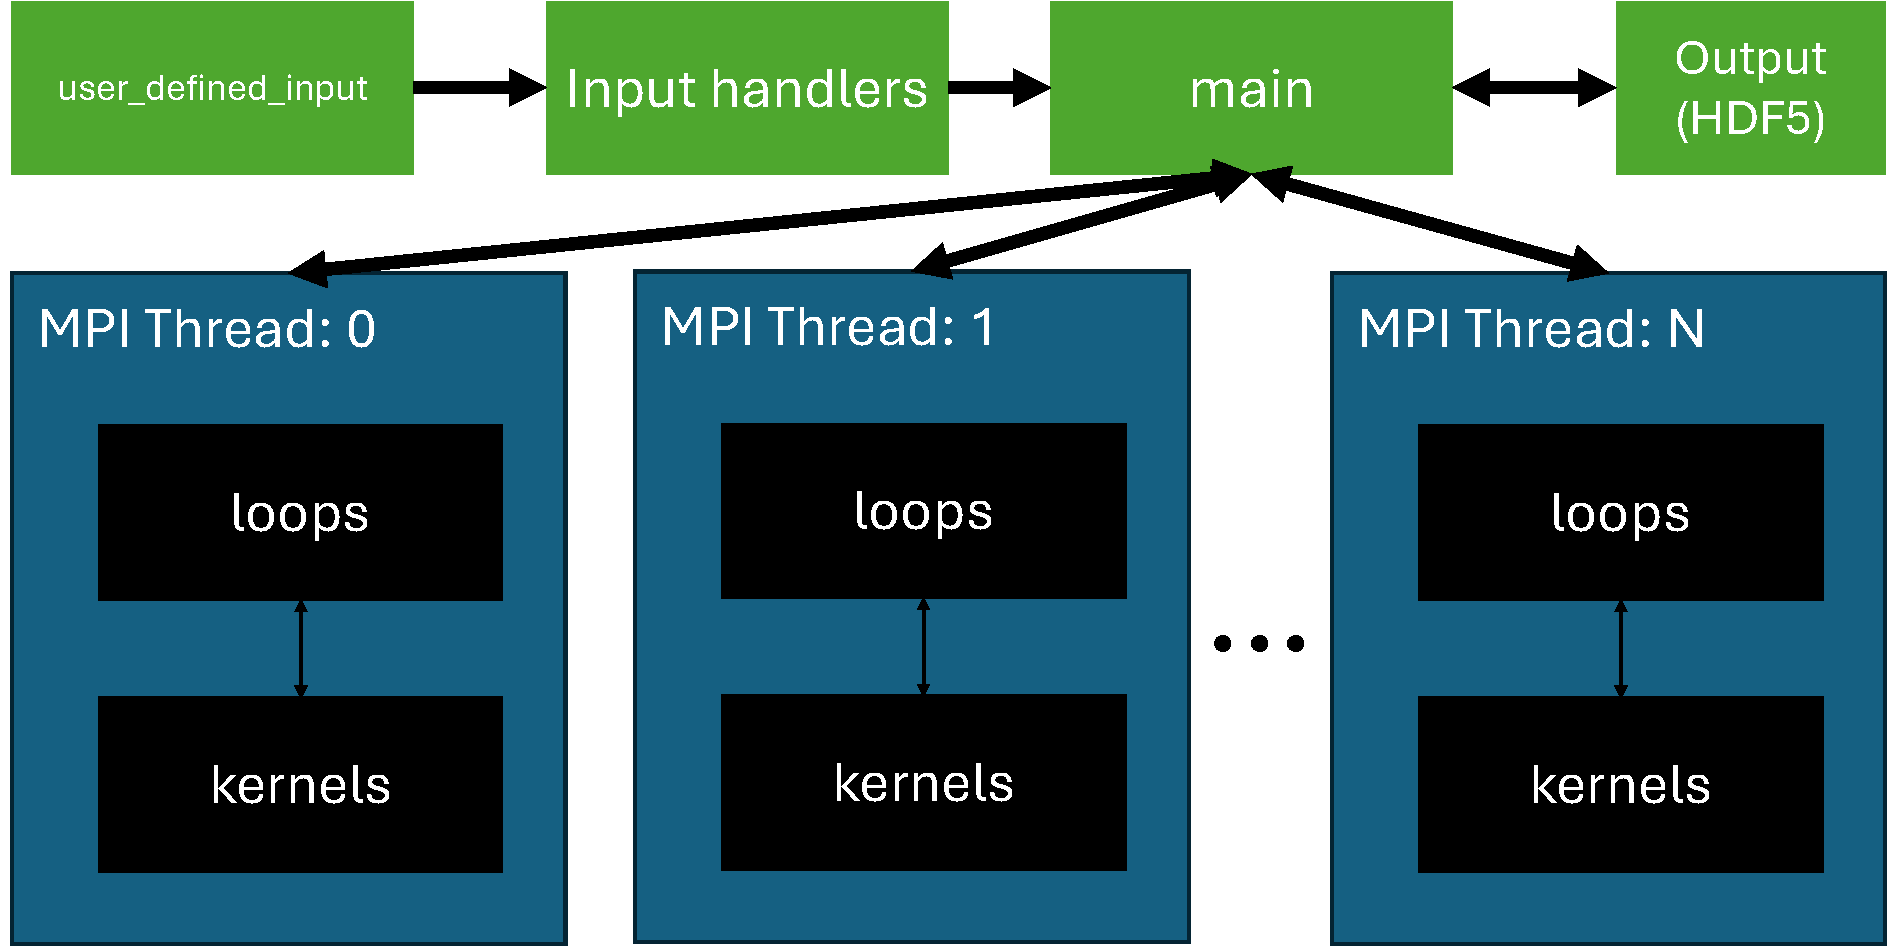
\includegraphics[width=.95\textwidth]{figures/cise_figs/flow.pdf}}
    \caption{MC/DC's overall structure and how functions get called and interact. Green functions are entirely Python, and black functions are compiled compute kernels if they are running in Numba CPU or GPU modes.}\vspace*{-5pt}
    \label{mpi_mcdc}
\end{figure*}

MC/DC offers a similar feature set as other Monte Carlo neutron transport applications (e.g., OpenMC \cite{romano_openmc_2015}, Shift \cite{hamilton_continuous-energy_2019}) with support for $k$-eigenvalue and fully time-dependent simulation modes in full three-dimensional constructive solid geometry.
It can model the neutron distribution in energy using either continuous energy or multigroup nuclear data.
It also supports domain decomposition.
All these features are supported on CPU (x86, ARM, POWERPC) and GPU processor targets (Nvidia and AMD), with MPI to target multiple processors (via mpi4py \cite{dalcin_mpi4py_2021}).

The number of novel schemes and simulation techniques implemented in MC/DC in a short time illustrates the success in its software engineering structure.
MC/DC supports the use of the iterative quasi-Monte Carlo (iQMC) method where deterministic and Monte Carlo transport operations run in tandem to converge solutions faster than they would in a pure Monte Carlo method. %\cite{pasmann_iqmc_nodate}
Other novel developments include global sensitivity analysis, hash-based random number generation for fully replicable solution testing, time-dependent population control, and continuously moving surfaces.
Several ongoing developments include quasi Monte Carlo, residual Monte Carlo, and machine learning techniques for dynamic node scheduling.

\section{MC/DC on CPUs}

To compile on CPUs, MC/DC uses the Numba compiler for Python to lower compute functions into LLVM and compile for a specific hardware target.
Figure~\ref{mpi_mcdc} shows MC/DC's functional layout when running in both MPI and Numba mode.

First, a user writes a Python script and imports \texttt{mcdc} as a package and forms an input script.
Then, the user interfaces with functions described in the input handler within MC/DC describing the physical models, material data, and simulation parameters.
This input layout is similar to how other Monte Carlo neutron transport applications input problems.

The input script calls a run command, which starts initialization functions within MC/DC. 
The initialization process allocates and constructs a global variable containing the user-defined inputs, meshes, particle banks, event tallies, and current global states.
This global variable is formed from a statically typed NumPy \texttt{ndarray}, which acts like a Python dictionary, where keywords are used to extract numerical arrays.
After building the global variable, initialization functions dispatch MPI processes if running in MPI mode, and begin the Monte Carlo neutron transport simulation.


Each MPI process calls functions containing the various transport algorithms and modes that MC/DC supports.
Each transport function is decorated with a Numba JIT (\texttt{@jit}) compilation flag declaring that each function must be compiled before being executed if running in Numba mode.
These transport logic loops are the highest level at which Python functions will be compiled in MC/DC.
For example, a fixed source problem will loop over all the particles and transport them until the particle's history is terminated from a physical event (e.g., capture, fission, time or space boundary), a simulation event (e.g., time census), or a variance-reduction event (e.g., population control, implicit capture).

The specific functions within each algorithm that conduct the actual transport operations (e.g., moving particles, tallying events, generating daughter particles from fission) are contained in the kernel set where all functions are \texttt{@jit} decorated.
Figure~\ref{fig:jitfunctions} shows an example compute kernel that updates the position and time of a particle as it moves.
It also shows the declaration of an \texttt{numpy.ndarray} data structure used in MC/DC.

\begin{figure}
\begin{minted}[mathescape, linenos]{python}
import numpy
from numba import jit

part = numpy.dtype([
    ('x', float64), ('y', float64),
    ('z', float64), ('ux', float64),
    ('uy', float64), ('uz', float64),
    ('v', float64) ])

@jit
def move_particle(P: part, distance):
    P['x'] += P['ux'] * distance
    P['y'] += P['uy'] * distance
    P['z'] += P['uz'] * distance
    P['t'] += distance / P['v']
\end{minted}
\caption{Example of a decorated function and MC/DC's data structures based on \texttt{numpy.ndarray}.}
\label{fig:jitfunctions}
\end{figure}

After all transport is completed and the simulation is finished, the program returns to the Python interpreter and calls finalization functions.
Here, requested tally information along with statistical error provided from the Monte Carlo process are saved in an HDF5 file.
Data can be extracted from this HDF5 file and used in Python scripts to do post-processing analysis and/or data visualization with tools like Matplotlib, or post-processing can be done in other applications like Visit or Paraview.

When initially exploring a novel transport method, a developer can work in a pure Python environment where functions are entirely executed in the Python interpreter.
In this mode, the developer can bring any package into any function, do typing dynamically, and use any Python data structure.
MC/DC can be executed in MPI mode in Python as well as compiled CPU mode.
While a full Python development environment is great for initially proving a concept, it often proves to be too slow for problems of interest.

When more performance is required, developers rewrite their kernels to strictly use Numba-enabled functions.
Numba only supports a small subset of the Python ecosystem. 
Some Python data structures like dictionaries and lists can no longer be used and must instead come from NumPy implementations. 
Thus, when using Numba, the small subset of functions supported effectively becomes a domain-specific language.

Scientific computing using Python is often done with NumPy functions and data structures, making these fairly natural for numerical-methods developers to use and understand.
In fact, we have found NumPy functionality to be more commonly used in initial development than other non-supported Python methods, making the restrictions in Numba more palatable.
Some developers report skipping Python-mode development entirely and starting with Numba-CPU work for their initial proofs of concept, as they find that aids in future debugging efforts.
Similarly, other developers report making small, incremental changes in Python-based algorithms, then checking to ensure successful compilation in Numba before moving forward, roughly at every commit.
When kernels are written to support Numba mode, they can be compiled to any supported CPU targets automatically (i.e., x86, ARM64, PPC64).

We can identify pitfalls with this approach, the most significant of which are:
\begin{itemize}
    \item Common failures of \texttt{numba.object\_mode},
    \item Lack of MPI calls from within the JIT-compiled Numba code,
    \item Numba kernel debugging and profiling;
    \item Loss of functions from SciPy not implemented in NumPy, and
    \item Restrictions with \texttt{numpy.ndarray} as our primary data structure.
\end{itemize}
Most of these issues have workarounds, but make implementing numerical methods in Numba harder.

Consider that \texttt{numpy.ndarray} requires ``square'' size allocation for all elements such that the size of every named element within an array must be the same.
If one element requires \num{10000} data points and the next only \num{100}, the size of that \texttt{numpy.ndarray} is \num{20000}, which is a drastic over-allocation.
This is a primary issue for continuous energy material data, where some materials may require tens of thousands of points to fully resolve, and others may only need hundreds.
While Numba does have some features to help in this circumstance (namely experimental \texttt{jit\_classes}), we must keep the \texttt{numpy.ndarray} to support MPI calls and GPU portability.
To fix this issue, given our constraints, we are moving towards using one-dimensional vectors with length information to offset between different variables, potentially impacting MC/DC's developer-friendliness.
Accepting increased complexity to achieve portability is common in MC/DC, so developing in it can be about as difficult as in a low-level language.

Other deficiencies are known to the Numba community, and some even have ongoing open-source remedies.
For example, \texttt{numba-mpi}\footnote{\url{https://github.com/numba-mpi/numba-mpi/}} is a project to support compiled-side MPI calls, \texttt{Profila}\footnote{\url{https://github.com/pythonspeed/profila}} attempts to bring the GNU debugger to Numba kernels, and \texttt{numba-scipy}\footnote{\url{https://github.com/numba/numba-scipy}} extends support for more SciPy functions to Numba.
However, most of these community projects are still in their infancy and not robust enough to handle the large and complex structures in MC/DC.

For CPU-based HPC deployments, a Python-as-glue strategy with Numba compute kernels can enable portable (between CPU architectures and scales) and high-performance code.
However, on GPUs, if using Python+Numba alone, a developer must still have in-depth understanding of their target GPU parallelism paradigm to achieve high performance.

\section{MC/DC on GPUs}

GPUs use a single-instruction multiple-thread (SIMT) parallelism paradigm, where threads are executed in teams called warps, or wavefronts, and do the same operations in lockstep. 
If threads in the same warp need to take different paths in a program (e.g., different if/else branches or iterating loops a different number of times), each path must be executed serially.
This behavior is called thread divergence.
Threads that do not belong to the currently executing path are disabled so that the end result of the computation is consistent with the control flow logic.
Mitigating thread divergence will usually result in higher performance of GPU-enabled applications.

Unfortunately, commonly implemented Monte Carlo neutron-transport algorithms are examples of highly divergent workflows, as the behavior of any individual particle is governed by random numbers.
Much more work is often required beyond naive syntax porting to implement Monte Carlo radiation transport applications to GPUs \cite{pozulp_progress_2023}.
When compiling and running on GPUs, MC/DC uses an open-source asynchronous event scheduling library called Harmonize\footnote{\url{https://github.com/CEMeNT-PSAAP/harmonize}}~\cite{brax2023} to 
reorganize the execution of business logic and storage/movement of data to better fit the SIMT execution paradigm of GPUs.
Harmonize implements runtimes that examine operations due to be executed, segregating them into like-operations so that like-work may be executed together in batches.

Monte Carlo transport functions lend themselves to asynchronous programming schemes, as it is intuitive to provide a function for each particle operation.
For example, Figure~\ref{fig:jitfunctions} shows a \texttt{move\_particle} function.
These functions can be ordered such that like operations get implemented in unison during runtime even if user defined control logic would dictate otherwise.
The end result of the computation is the same, but the order of execution on the processor has been optimized.
MC/DC calls Harmonize via Python bindings.
Harmonize has been shown to increase GPU performance by reducing thread divergence \cite{brax2023}.


\begin{figure}
\begin{minted}[mathescape, linenos]{python}
from numba import cuda

@for_cpu
def add(array, value, idx):
    array[idx] += value

@for_gpu
def add(array, value, idx):
    cuda.atomic_add(array, value, idx)

def tally_collision_event(mcdc, part):
    id = loc2index(part)
    add(mcdc.col_tally, part.v, id)
\end{minted}
\caption{Example of GPU and CPU specific API calls as defined in MC/DC and their use in a collision tally function.}
\label{fig:forcpuvgpu}
\end{figure}

% description of GPU mode execution
Moving to compile and run Numba \texttt{jit}ed functions to the GPU requires making a few alterations to the kernels themselves.
An even-smaller subset of Python functions work in GPU-compiled code, with operations supported on Numba-CPU like \texttt{numpy.linalg.solve()} losing support.
Other operations may require API-specific calls, exposed by Numba commands.
For example, atomic operations are required to preserve the side-effects of individual threads acting on global memory (e.g., adding to a tally).
To allow for a mostly unified kernel base in MC/DC for both CPUs and GPUs, we track alternate function implementations registered through decorators.

Figure~\ref{fig:forcpuvgpu} shows how we implement alternate tally accumulation functions using \texttt{@for\_cpu} and \texttt{@for\_gpu} decorators.
Here \texttt{@for\_cpu} adds one to a value in an array, and since this is within a single MPI rank we can assume a thread-safe operation.
However, on the GPU this may result in a memory race condition requiring an \texttt{numba.cuda.atomic\_add} API call.
While this does increase complexity for a programmer implementing numerical methods, it is nowhere near the complexity that might be required to accomplish a similar implementation in a compiled language.

Most numerical methods development in MC/DC is done by editing pre-existing control flow (e.g., adding more operations or device functions to existing loops, adding more components to a data structure).
Once all alterations can compile and execute using Numba-CPU functionality and necessary API calls have been abstracted, MC/DC and Harmonize automatically compile and execute those extra commands on GPUs.
So, in most cases, methods developers do not need to interface with Harmonize commands or make any alterations to the GPU runtime, data management, or compilation techniques.

If more-significant alterations are required for a given numerical method, a developer may have to interface directly with Harmonize.
We have found that, for the majority of our work exploring new algorithms to date, Harmonize+Numba sufficiently abstracts the SIMT parallelism paradigm such that operations that work on the CPU side are generally supported on GPU with little effort from the methods developer.

% descirption of compilation + harmonize
To compile functions to GPU targets with Harmonize, Numba generates intermediate compiler representations (IRs, e.g., LLVM-IR or PTX) of Monte Carlo neutron transport kernels. 
Harmonize then ingests and links those IRs with the event-scheduling runtime.
MC/DC's documentation\footnote{\url{https://mcdc.readthedocs.io/en/dev/theory/gpu.html}} provides a more in-depth description how MC/DC and Harmonize are JIT compiled for given hardware.

When running MC/DC in GPU mode on an individual MPI thread, MC/DC+Harmonize is first JIT compiled, then  during initialization allocates device memory for the global array and moves this from the host (CPU) to the device (GPU).
Next, MC/DC's transport kernels are executed with Harmonize on the GPU until transport for a given collection of work is complete.
Communication between the GPU and CPU of the global variable may be required during transport for some simulation modes.
When transport is finished, the global variable moves back to the host for a final time, and the simulation completes.
% workflow description

Just as with CPU development, this abstraction strategy has some potential disadvantages.
While MC/DC's software engineering structure allows for kernel portability between CPUs and GPUs significant time and effort can be lost in debugging, particularly for the data structures.
MC/DC only operates on GPUs using Harmonize.
Beyond its event scheduling and runtime capabilities, Harmonize allows us to ameliorate issues in Numba's GPU feature set.
For example, allocating and moving data from the CPU to GPU can only happen from Python code and cannot be done from Numba-compiled CPU kernels (requiring an \texttt{object\_mode} call).
In our initial implementations this required many copies of the global variable, which proved prohibitively costly for larger problems.
Using API calls elevated through Harmonize instead of Numba fixes this issue, requiring only two copies of the data, and the data can be accessed from both Numba-compiled CPU and GPU kernels.
In addition, when extending GPU operability to other vendors (namely AMD GPU support), Harmonize allows us to elevate non-implemented Numba API calls to the MC/DC Python interface.
For example, the Numba-HIP package\footnote{\url{https://github.com/ROCm/numba-hip}} does not currently support atomic operations on vectors.
Harmonize provides a clear path to elevate HIP-C\texttt{++} functions into Python for use in MC/DC.

For GPU development, the portability and performance enabled by MC/DC's software engineering structure increases the difficultly of implementation for the workflow developer who actually interfaces with Numba and Harmonize.
Our hope is that the investment made by the workflow developers is compounded with rapid development of more numerical methods.


\section{Performance}
\label{sec:cise:performance}

\begin{figure}
    \centerline{
    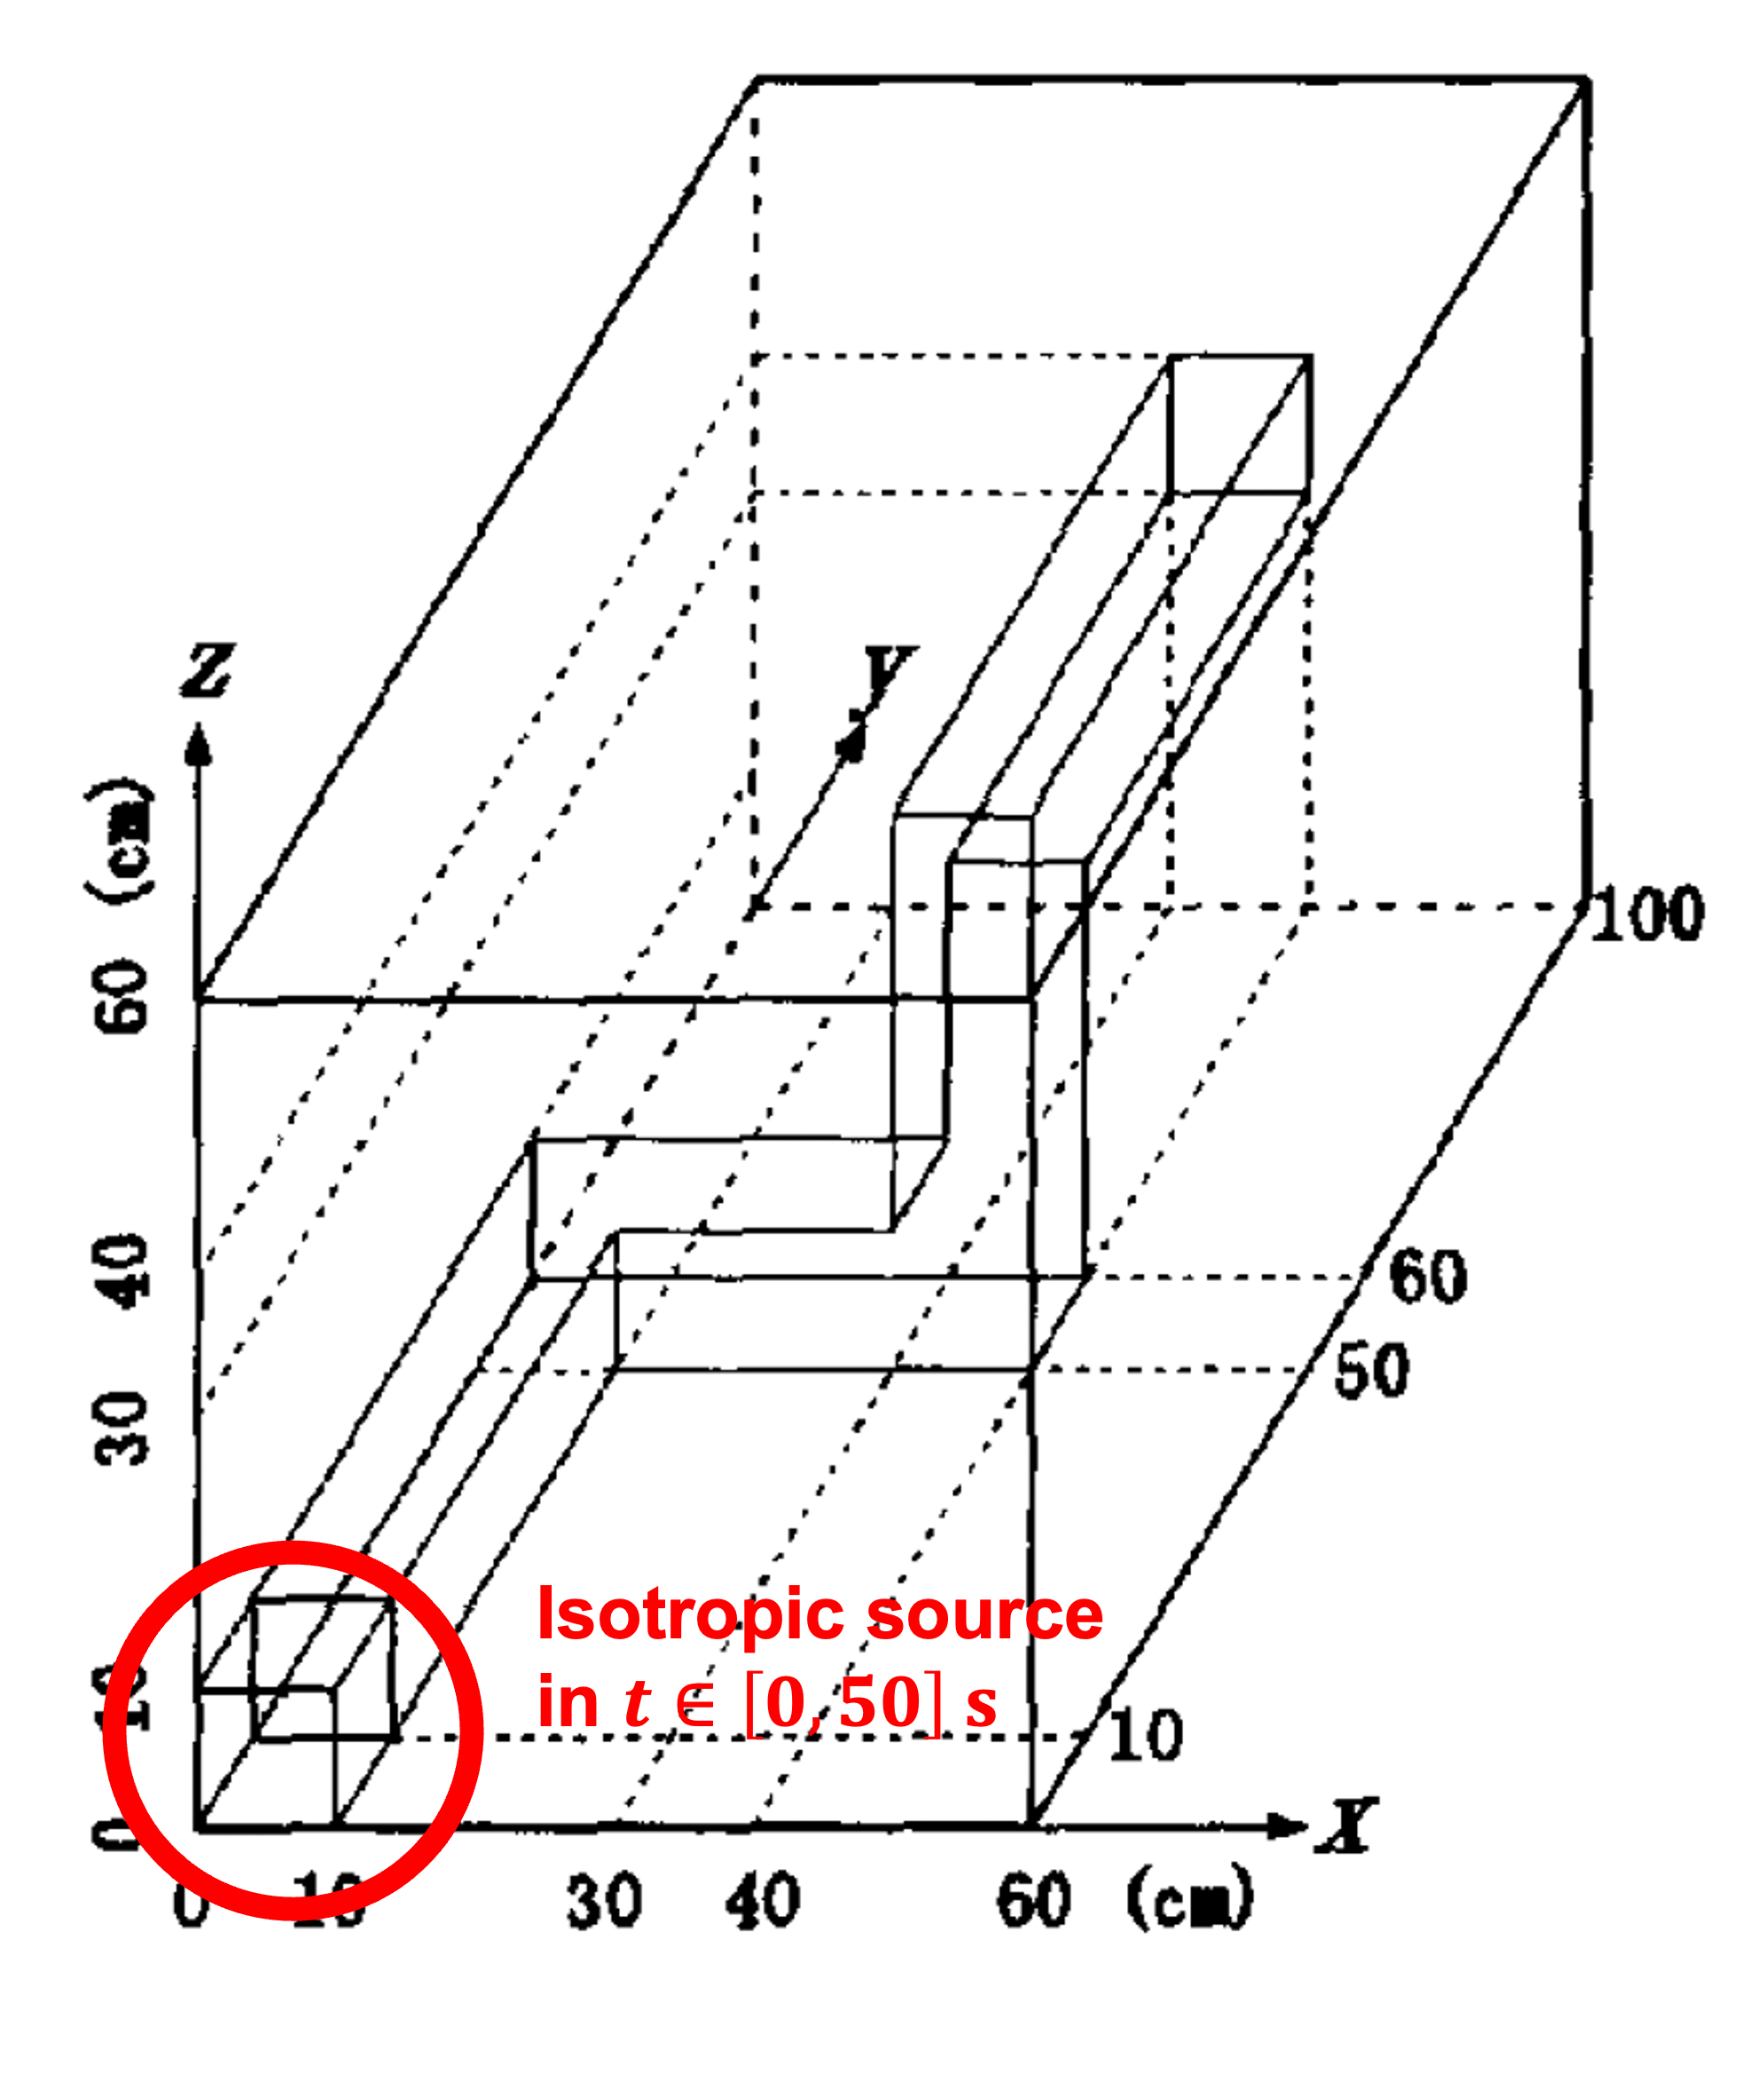
\includegraphics[width=.4 \textwidth]{figures/cise_figs/kobayashi_problem.png}
    } 
    \caption{Kobayashi problem schematic.}
    \label{koby-problem-def}
\end{figure}

\begin{figure*}[h]
    \centerline{
    %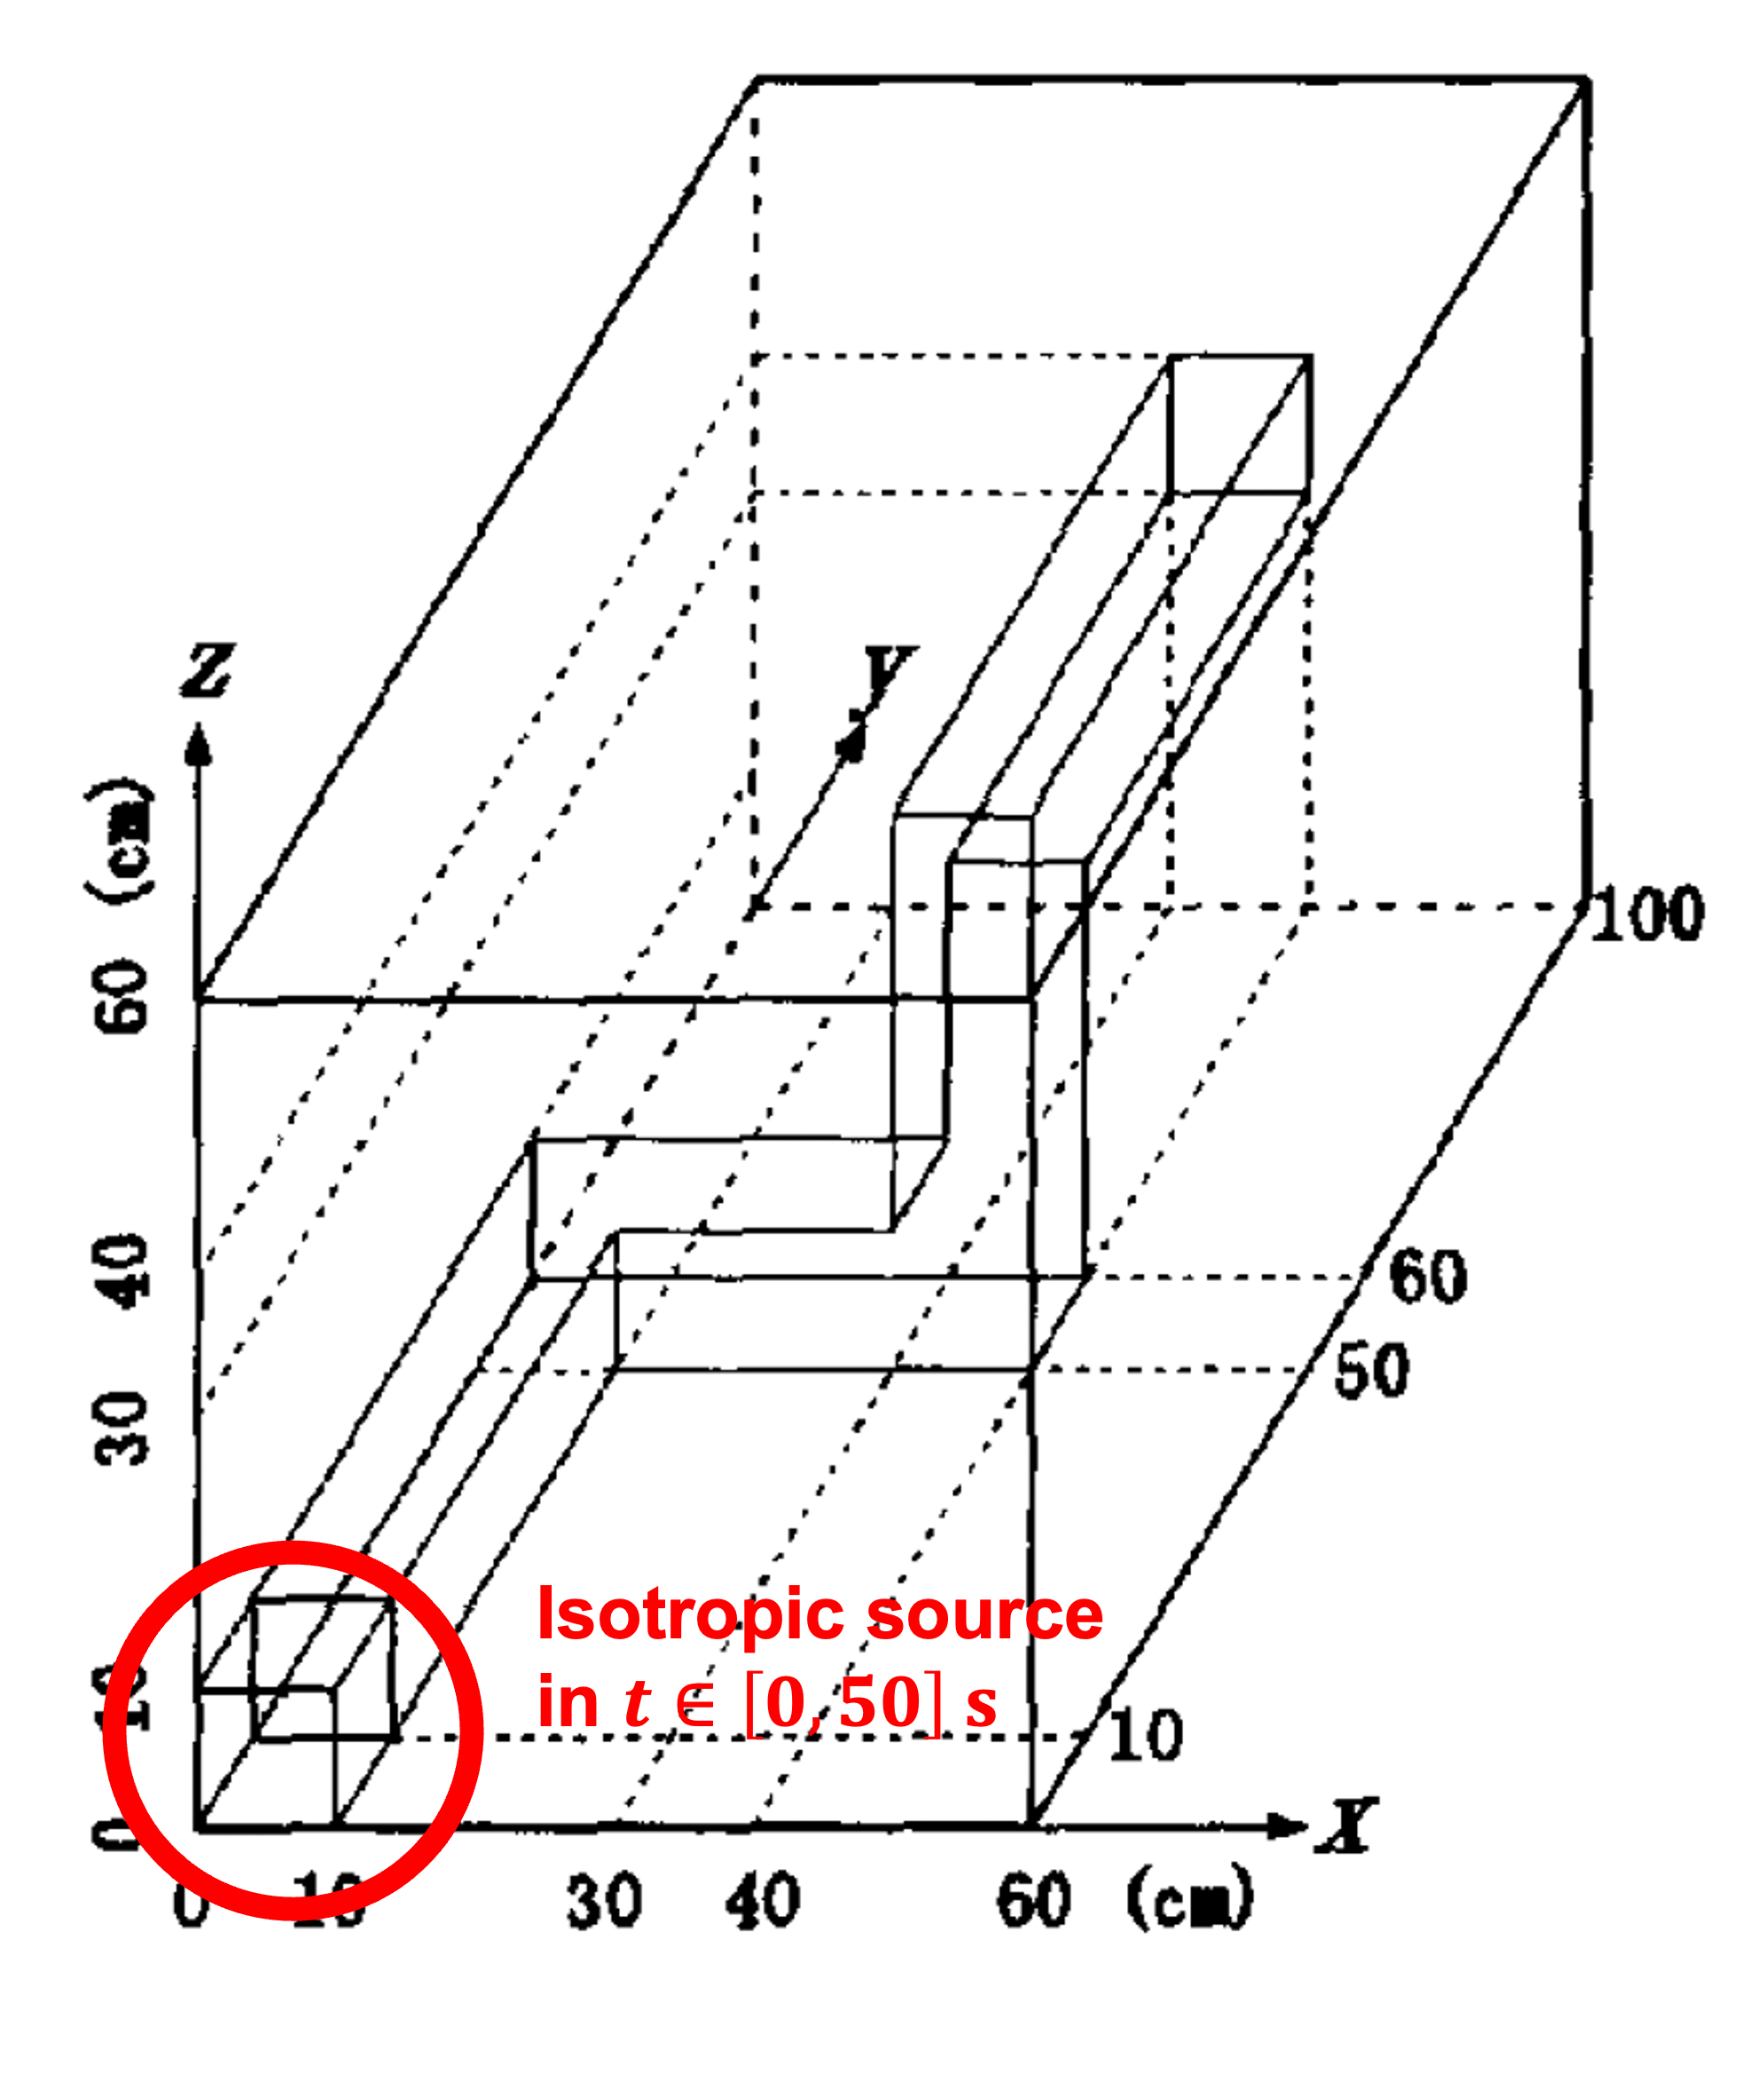
\includegraphics[width=.3\textwidth]{figures/cise_figs/kobayashi_problem.png} \hspace{1cm}
    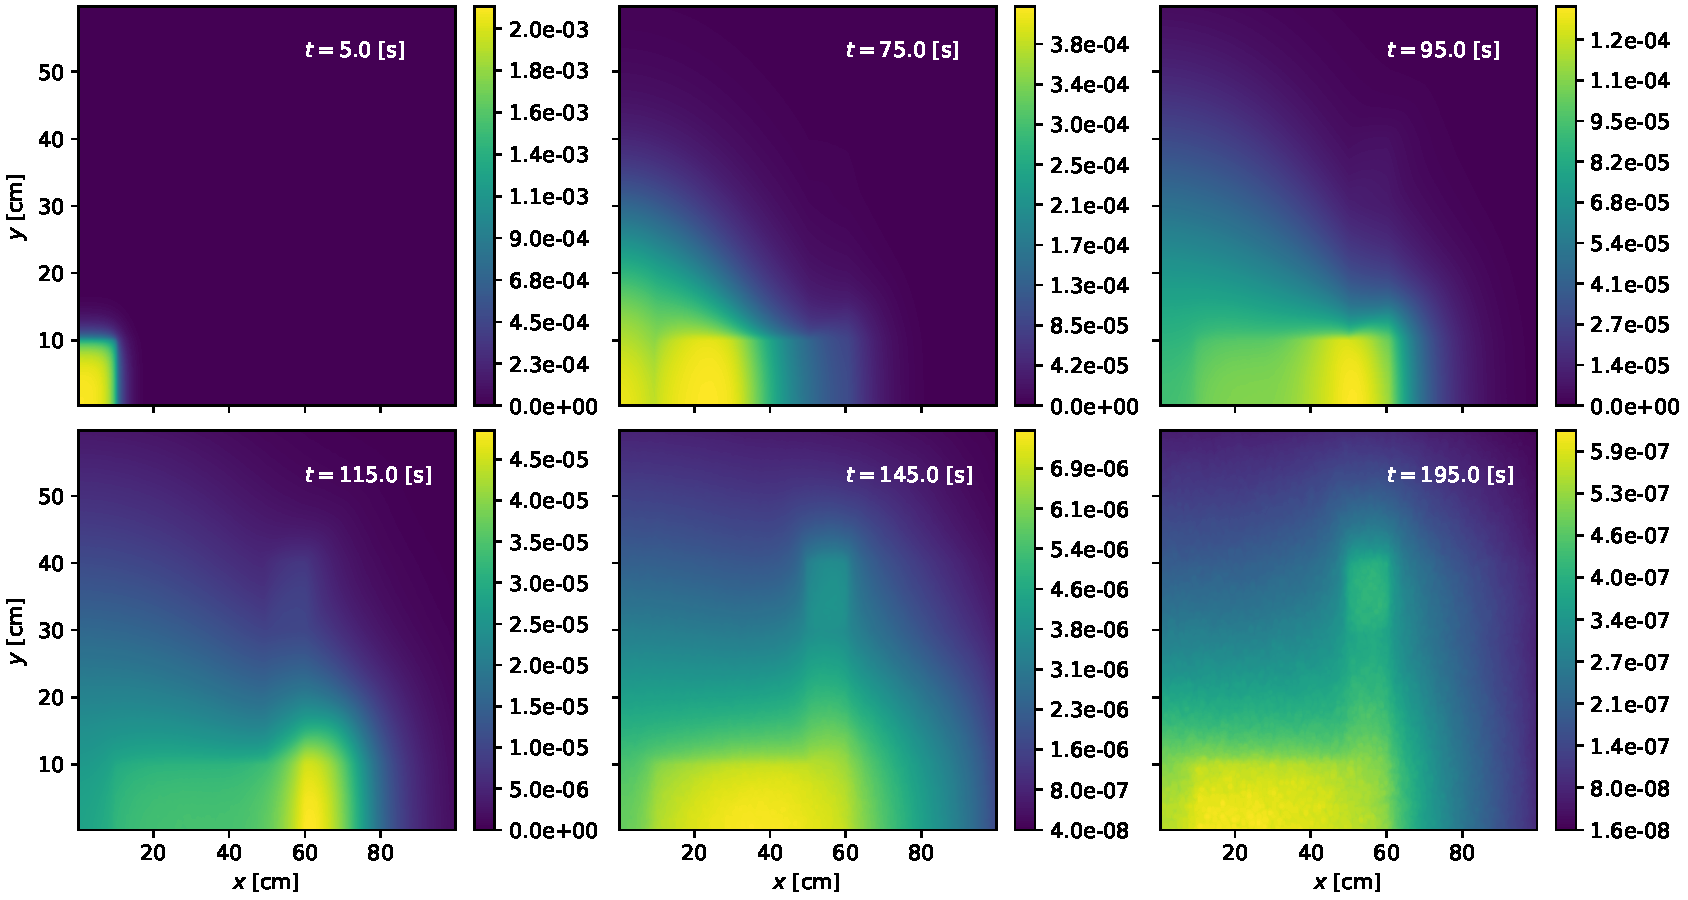
\includegraphics[width=\textwidth]{figures/cise_figs/koby.pdf}
    } 
    \caption{Time and space averaged scalar flux solution to the Kobayashi problem run with $1\times 10^{9}$ particle histories at various points in time.}
    \label{koby-results}
\end{figure*}

% transient runtime strong scaling mcdc v openmc maybe v shift?
To examine the performance of MC/DC we use a time-dependent version of the one-group Kobayashi dog-leg void-duct problem \cite{Kobayashi2001, variansyah_mc23_mcdc}.
Figure~\ref{koby-problem-def} shows the void duct and the location of the neutron source at the opening of the duct.
The initial condition is zero flux everywhere.
Radiation quickly moves through the void and then penetrates the walls of the problem, slowly dissipating through time.
Figure~\ref{koby-results} shows the duct clearly with the scalar flux solution at various points in time.

We solved the Kobyashi problem on HPC systems available at Lawrence Livermore National Laboratory (LLNL): the Dane and Lassen machines.
Dane is a CPU-only system with dual-socket Intel Xeon Sapphire Rapids CPUs, each with 56 cores for a total of 112 per node.
Lassen has four Nvidia Tesla V100s and two IBM Power 9 CPUs per node.
To contrast MC/DC on the CPU against a traditionally developed and compiled code, we will compare performance to another Monte Carlo neutron transport code, OpenMC\footnote{\url{https://github.com/openmc-dev/openmc}} \cite{romano_openmc_2015} (an open-source code written in C\texttt{++}).
We added time-dependent functionality to OpenMC\footnote{\url{https://github.com/CEMeNT-PSAAP/openmc/tree/transient}} so that the same algorithm is implemented in both codes for the Kobyashi problem.


Figure~\ref{performance_results} at left shows the wall-clock runtime of OpenMC (112 MPI threads), MC/DC-CPU (112 MPI threads), and MC/DC-GPU (four MPI threads) using all available resources of a given node type.
Both MC/DC runs are JIT compiled, which means compiling consumes a considerable amount of wall-clock runtime for even small problems (about \SI{70}{\s} and \SI{140}{\s} for CPU and GPU targets, respectively).
For small particle counts, actual compute time is small relative to compile time, so both MC/DC lines are flat until enough work saturates the computational power of a given resource---around \num{e8} particles for MC/DC-CPU and \num{e9} for MC/DC-GPU.
At full saturation (\num{e10} particles) MC/DC-CPU runs about 22\% slower than OpenMC, while MC/DC-GPU is 8$\times$ faster than MC/DC-CPU and 6$\times$ faster than OpenMC.

OpenMC displays superior performance at smaller particle counts due to it being a fully compiled code.
GPU profiling for MC/DC shows that
\texttt{memalloc} and \texttt{memcopy} CUDA API calls 
occupies 2.2\% of runtime (\SI{32.8}{\s} out of \SI{1500}{\s})
when running \num{e10} particles on one Lassen GPU for the Kobyashi problem.
At \num{e9} particles, GPU memory commands account for 11.8\% of runtime (\SI{18.0}{\s} out of \SI{147.0}{\s}).


Figure~\ref{performance_results} at right shows weak-scaling performance (\num{e10} particles per node) with the Kobyashi problem for MC/DC-CPU (Dane), OpenMC (Dane), and MC/DC-GPU (Lassen).
Each node is using all available compute resources for a given calculation (e.g., four nodes is 480 CPU cores and 16 GPUs on Dane and Lassen, respectively).
MC/DC-CPU shows a minimum efficiency of \num{0.85} at 256 nodes while OpenMC only falls to \num{0.89}.
OpenMC supports shared-memory parallelism (using OpenMP) but these calculations only use domain-replicated MPI.
MC/DC-GPU shows the best weak-scaling efficiency for this problem, decreasing only to \num{0.95} at 256 nodes.

\begin{figure*}[h]
    \centerline{
    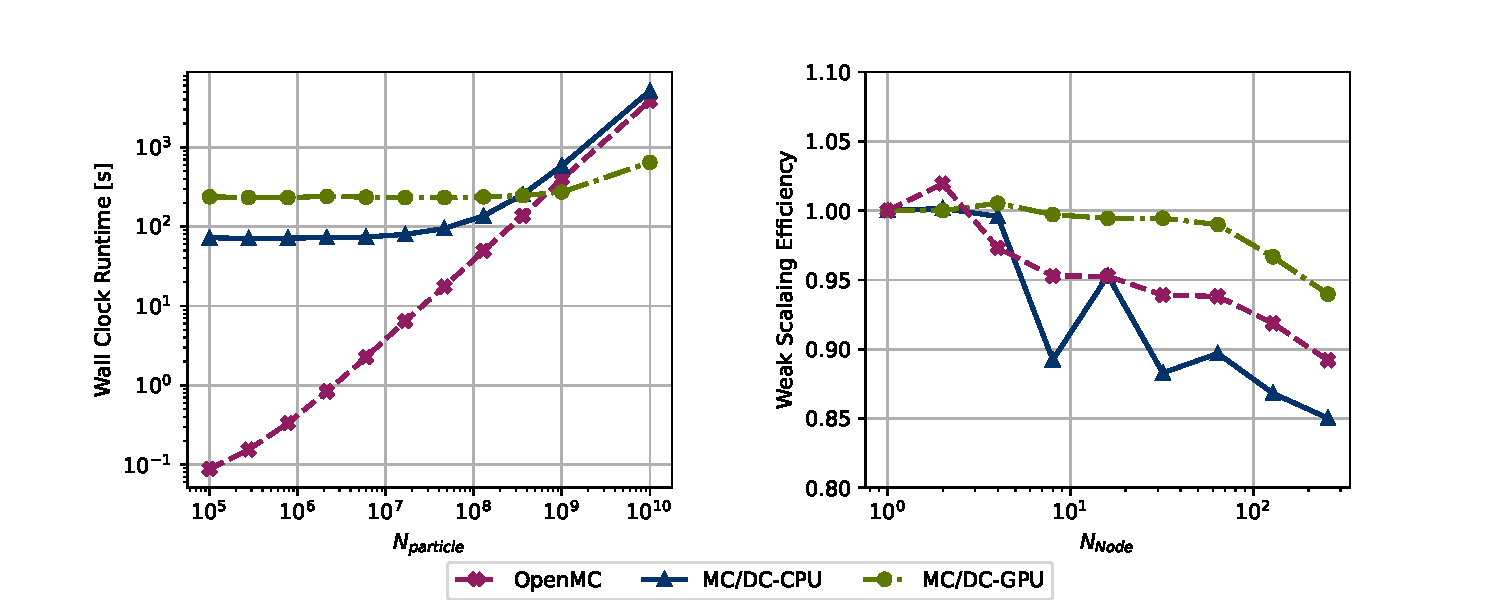
\includegraphics[width=1.1\textwidth]{figures/cise_figs/comps.pdf}
    }
    \caption{Left: Wall-clock runtime of the Kobyashi problem over particle counts. 
    Right: Weak scaling efficiency as a function of node count for the Kobyashi problem on Dane (CPU) and Lassen (GPU).}
    \label{performance_results}
\end{figure*}

\section{Discussion, Conclusions, and Future Work}

Monte Carlo/Dynamic Code (MC/DC) is a Monte Carlo neutron transport code that targets modern HPC architectures with CPUs and GPUs.
Our performance results demonstrate that MC/DC's structure using a Python + Numba + MPI + Harmonize scheme can produce similar performance to other Monte Carlo neutron transport solvers.
After JIT compilation overhead, MC/DC performs similarly to traditionally compiled production code on a single node for a transient problem of interest.
MC/DC exhibits similar weak scaling on CPUs and superior weak scaling on GPUs up to 256 nodes of a given HPC, compared with a CPU-only production code.

Developing using Numba for CPU targets can be as difficult as developing in low-level languages for the complicated algorithms we implement. 
This agrees with previously published analysis \cite{KailasaSrinath2022PAEi}.
We found developing the necessary time-dependent features to model the Kobyashi problem in OpenMC to be about as difficult as making changes within MC/DC.
For our application, anything gained when using a high-level-language is lost in time and effort spent circumventing unsupported operations and debugging. 
However, the implementation in OpenMC remains CPU-only, while for MC/DC it took little effort to go from a working CPU implementation to something operating and highly-performing on GPUs.
Of course, we use our own specialized event-scheduling library to do this---but Numba allows us to construct a Python-based portability framework fit to our numerical method with the added benefit of unifying our high-level glue language and kernel-production language.

Over the duration of developing MC/DC (starting in 2021) we have seen many improvements to Numba.
Compiler error reporting continues to improve (especially in Numba versions 0.59.0$+$), the number of supported operations have grown, and Numba has been extended to additional accelerators like AMD and Intel\footnote{\url{https://github.com/IntelPython/numba-dpex}} GPUs.
We have found that the Numba development team fosters a supportive community that is approachable and responsive to questions, comments, and concerns.
We believe that as Numba matures we will continue to see performance and development improvements.

Work in MC/DC is ongoing.
We are continually exploring novel variance reduction and hybrid Monte Carlo techniques, and adding new functionality.
For GPU development specifically we are currently investigating use of unified memory between the CPU and GPU as well as extending support to Intel GPUs.
We will continue to improve MC/DC, making it a portable application for rapid methods development enabled by Python and Numba.

\section{Acknowledgments}
The authors thank the Numba development team for support using the Numba compiler as well as Damon McDougall and Dominic Etienne Charrier from Advanced Micro Devices for support using Numba-HIP and ROCm compilers.
The authors thank the high performance computing staff at Lawrence Livermore National Laboratory for continued support using the Dane and Lassen machines.

This work was supported by the Center for Exascale Monte-Carlo Neutron Transport (CEMeNT) a PSAAP-III project funded by the Department of Energy, grant number: DE-NA003967.
\newpage
\renewcommand{\TheTitle}{Hybrid Woodcock-delta Tracking Schemes Using a Track-Length Estimator}
\renewcommand{\TheAuthors}{Joanna Piper Morgan,
  Ilham Variansyah,
  Kayla B. Clements,
  Todd S. Palmer,
  Kyle E. Niemeyer,}

\renewcommand{\TheAddress}{
\textit{Submitted to Journal of Computational and Theoretical Transport} \\

}

\PaperHeader{\TheTitle}{\TheAuthors}{\TheAddress}

\chapter{\TheTitle}
\label{chap:delta_tracking_paper}

\epigraphhead[10]{\singlespacing
    \epigraph{
        And it's knowing I'm not shackled\\
        By forgotten words and bonds\\
        And the ink stains that are dried upon some line\\
        That keeps you in the back roads by the rivers of my memory\\
        That keeps you ever gentle on my mind\\
    }
    {Glenn Campbell}
}

\newcommand{\maj}{\Sigma_{\text{maj}}}

%%% Write text for abstract
%%% Most text modifying commands will work in abstract

\section*{Abstract}

Woodcock-Delta tracking is a common alternative to the more popular surface tracking technique where the largest cross-section at a given energy in the whole problem is used to sample a distance to collision at any point.
This process forces extra nonphysical collisions so it is paired with a rejection sample to determine real events from virtual or phantom events.
Traditional implementations of Woodcock-delta tracking preclude the use of a track (or path-) length estimator for scalar flux tallies and are forced to use the normally higher-variant collision estimator instead.
There is no mathematical reason why the track-length estimator cannot be used in conjunction with Woodcock-delta tracking only implementation issues. 
In this work we take advantage of that to produce a Woodcock-delta tracking algorithm which tallies fluxes to a structured rectilinear mesh using the track-length estimator.
This development more readily enables hybrid surface-delta tracking algorithms as the track-length tally can be used everywhere for scalar flux estimation regardless of which tracking algorithm a particle is using.
We use this when developing a novel hybrid-in-energy method where Woodcock-delta tracking is used in high energies (where mean free paths are long) and surface tracking below that (starting at the neutron resonances) as well as a previously defined hybrid-in-material method.
We verify that delta tracking algorithms we consider can be used in conjunction with continuously moving surfaces.
We benchmark these methods showing figures of merit on four time-dependent problems: two multi-group and two continuous-energy.
Woodcock-delta tracking with a track-length tally showed modest improvements to figures of merit as compared to traditional delta tracking with a collision estimator and surface tracking with a track-length estimator (\num{1.5}$\times$--\num{2.5}$\times$) and significant improvements (\num{7}$\times$--\num{11}$\times$) when using the hybrid-in-energy method.

\section{Introduction}

% general introduction
Predicting the neutron distribution in space, energy and time is important when modeling inertial confinement fusion systems, pulsed neutron sources, and nuclear criticality safety experiments, among other systems.
The behavior of neutrons can be modeled with a Monte Carlo simulation, where particles with statistical importance are created and transported to produce a particle history \cite{lewis_computational_1984}. 
The path of a particle and the specific set of events that occur within its history are governed by pseudorandom numbers, known probabilities (for example, from material data), and known geometries. Data about how
particles move and/or interact with the system are tallied to compute parameters of interest with an associated statistical error from the Monte Carlo process.

There are two common methods used to sample the random walk in a Monte Carlo neutron transport algorithm: surface tracking \cite{lewis_computational_1984} and Woodcock-delta tracking \cite{woodcock_techniques_1965}.
These two tracking algorithms have complementary performance bottlenecks, for a certain class of problems, a hybrid method may allow for greater performance than either approach used individually.
For example: traditional implementations of Woodcock-delta tracking preclude evaluating quantities of interest with a track-length estimator instead opting for a collision estimator may be used, whereas, surface tracking has no such restrictions.
The track-length estimator usually provides a better estimate of quantities of interest (see section \ref{sec:tracking_algs_and_est}).
On the hand, surface tracking requires potentially complicated geometric operations whereas Woodcock-Delta tracking does not.
Which method to use is often problem dependent.

% cite previous M&C paper

Previous work into delta-surface tracking on a structured mesh has shown good performance for problems with complex arrangements of optically-thin materials\cite{morgan2023delta}.
Making material-based decisions about when to do delta and surface tracking has also been explored and implemented in production Monte Carlo codes \cite{leppanen_development_2013conf, leppanen_2010_burnup, richards_monk_2015}.
We extend the idea of \textit{tracking} on a structured mesh to full Woodcock-delta tracking (eliminating the distance to surface check) and \textit{tallying} to a structured mesh allowing the use of a track-length estimator for estimations of scalar flux.
% MC/DC introduction

In this work we describe, verify, and evaluate the performance of a delta tracking algorithm that allows the use of a track-length estimator on a structured tally mesh.
We then use this approach in two hybrid delta tracking schemes: one in which the choice tracking algorithm is based on material region, and another scheme based on the particle energy.
We implement this work in Monte Carlo Dynamic Code (MC/DC), an open source Monte Carlo neutron transport application purpose-built to conduct rapid numerical methods development, specifically for time-dependent problems \cite{morgan_monte_2024}.
We compute figures of merit for four computationally difficult benchmark problems including a stuck rod accident simulation of a continuous energy version of the C5G7 geometry, and runtime results for a whole CPU node (2X Intel x86 Xeon Sapphire Rapids) and a whole GPU Node (4X Nvidia Tesla V100).

This work is novel as it is the first published usage of a track-length estimator for scalar flux estimation with full Woodcock-delta tracking, the first usage of Woodcock-delta tracking in conjunction with continuously moving surfaces (implemented in MC/DC \cite{variansyah_2023_highfidelity}), and the first time a hybrid delta tracking method has been based on the energy of a given particle.
The quantities of interest in this work are estimates of scalar flux and not full reaction rate densities for all particle material interactions.
While this does limit the generally applicability of these methods, scalar flux is a necessary quantity for hybrid methods, and other uses.
Indeed for deterministic method if scalar flux is ascertained the problem is considered solved.


\section{Tracking Algorithms and Estimators}
\label{sec:tracking_algs_and_est}

% Surface tracking
To track the movement of neutrons within a system and, one of two tracking (or sampling) methods are employed. 
The first is surface tracking described in algorithm \ref{alg:surface}. 
For a particle in material $m$, a distance to collision is sample from a cumulative probability distribution function by
\begin{equation}
    d_{\text{collision}} = \frac{-\ln(\xi)}{\Sigma_{t,m}} \; ,
\end{equation}
where $\Sigma_{t,m}$ [\SI{}{\per\centi\meter}] is the macroscopic total cross section of the $m$-th material and $\xi$ is a pseudo-random number between zero and one.

This sampling of the cumulative probability distribution function will only hold true while the material is homogeneous.
So if the distance to collision is beyond a material interface in a system with multiple materials, the particle must be stopped at that interface surface and a new distance to collision must be calculated with with the new material's $\Sigma_{t,m}$.
This approach is an unbiased way of dealing with the sampling of distance to collision in a heterogeneous medium.
In a standard surface tracking algorithm this involves computing both a distance to collision ($d_{\text{collision}}$) and a distance to the nearest surface along the particle's direction of travel ($d_{\text{surface}}$).
The smaller of these two distances determines which event happens to the particle - a collision or a surface-crossing.
After or while the particle is moving, tallies can be accumulated to compute quantities of interest.
If a collision occurs, more sampling and operations can be done (e.g., isotropically scatter a particle).
If the particle is still alive at the end, the algorithm is repeated.
The distance to nearest surface computation can become quite expensive as geometries grow in complexity (e.g. complex CSG geometries or CAD based surfaces).
Surface tracking is at the heart of many modern Monte Carlo neutron transport applications, including MCNP \cite{MCNP_RisingArmstrongEtAl}, Shift \cite{hamilton_continuous-energy_2019, pandya_implementation_2016}, MONK/MCBEND \cite{richards_monk_2015}, and OpenMC \cite{romano_openmc_2015}.


\begin{algorithm}
\begin{algorithmic}[1]
    \State $m =$ lookup material in current particle location

    \State $\Sigma_{t,m} =$ look up total macroscopic cross section of material $m$ 

    \While{particle is alive}
    
        \State $d_{\text{collision}} = -\ln{\xi} / \Sigma_{t,m} $
        
        \State $d_{\text{surface}} =$ compute distance to nearest surface along particle direction of travel

        \If{$d_{\text{collision}} < d_{\text{surface}}$}

                \State $d = d_{\text{collision}}$
                
                \State sample collision type
                
                \State carry out collision
                
            \Else 

                \State $d = d_{\text{surface}}$
        
                \State move particle to surface
    
                \State $m =$ lookup material on the other side of the surface
    
                \State $\Sigma_{t,m} =$ look up total macroscopic cross section of material $m$ 
    
                \If {surface is a boundary}
    
                    \State implement boundary condition
    
                \EndIf
        \EndIf
        \State score track-lengths to tally bins
    \EndWhile
    \caption{A generic surface tracking algorithm.}
    \label{alg:surface}
\end{algorithmic}
\end{algorithm}


Delta tracking is the next most common tracking approach and is shown in algorithm \ref{alg:trad}.
It starts by pre-processing a \textit{majorant} macroscopic cross-section
\begin{equation}
    \maj(E) = \max\left({\Sigma_{t,1}(E), \Sigma_{t,2}(E) \dots \Sigma_{t,m}(E) \dots \Sigma_{t,M}(E)}\right)
\end{equation}
such that it is the largest cross section at any given point in any material in the problem.
The algorithm to compute the majorant cross-section for nuclides on a non-unified energy grid currently implemented in MC/DC is in appendix \ref{app:majorant}.
Figure \ref{fig:majorant_c5ce} at right shows a macroscopic majorant cross section for a typical pressurized water reactor.
When delta tracking the distance to collision is always computed with the majorant,
\begin{equation}
    _{\text{collision}} = \frac{-\ln{\xi}}{\maj} \; ,
\end{equation}
ignoring surface crossing events.
However, this sampling forces extra collisions that do not physically exist; using the majorant generates the smallest distance to collision. Delta tracking algorithms use a rejection sampling to determine if the sampled collision event was \textit{real} or a \textit{virtual} (\textit{phantom}) collision.
At the particle's current location, the true material region of the is be identified to compute $\Sigma_{t,m}$.
If 
\begin{equation}
    \xi > \frac{\Sigma_{t,m}}{\maj} \; ,
\end{equation}
where $\xi$ is a new random number, the collision did not physically occur, is rejected, and the particle can be left alive on it's current direction of travel and energy.
From here the process is the same as before: tallies are accumulated, real collision physics are carried out when appropriate, and the algorithm continues as long as the particle is still alive.

\begin{figure}
    \centering
    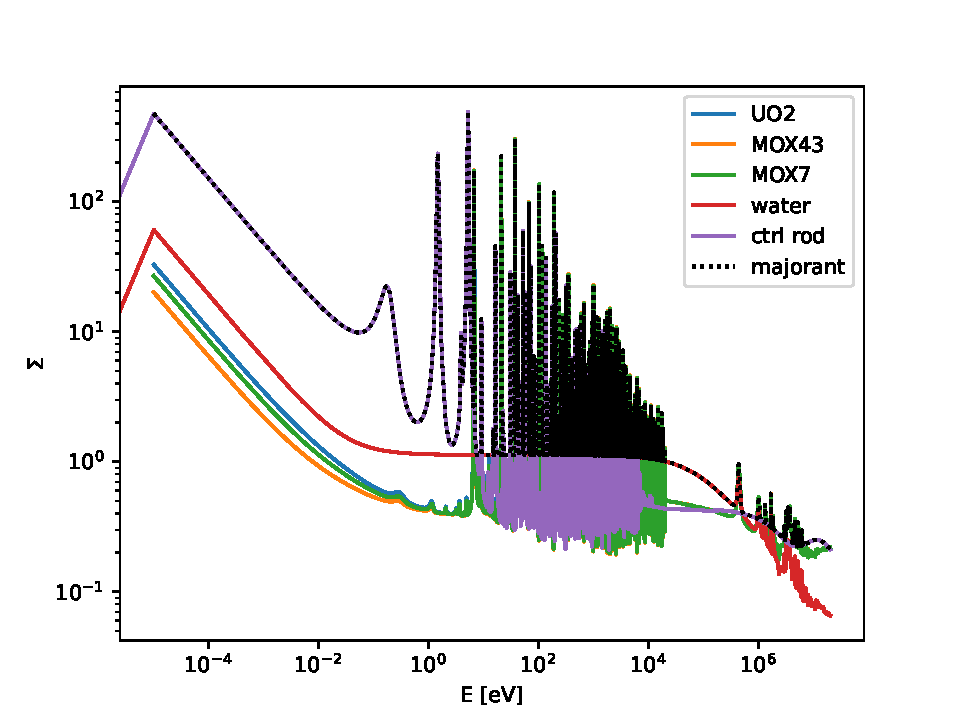
\includegraphics[width=0.75\textwidth]{monte_carlo/delta_tracking/figures/macro_majorant_c5ce.pdf}
    \caption{Continuous energy macroscopic majorant cross-section ($\maj$) for the continuous energy version of C5G7 PWR described in appendix \ref{app:c5ce_mat}.}
    \label{fig:majorant_c5ce}
\end{figure}

When undergoing delta tracking some way to kill or reflect particles on vacuum or reflecting boundary conditions respectively is needed.
In a code that already implements surface tracking, the functionality to track distances to specific surfaces will already exist.
So it is natural when undergoing delta tracking to only compare distances to boundary surfaces exclusively.
Boundary surfaces are often planar, making the computation trivial and cheap.
%This is similar to other methods currently under development in OpenMC.

\begin{algorithm}
\begin{algorithmic}[1]
    \While{particle is alive}
        \State $d_{\text{collision}} = -\ln{\xi} / \maj $
        \State $d_{\text{boundary}} =$ compute distance to boundary
        
        \If {$d_{\text{collision}} < d_{\text{boundary}}$}
            \State $m =$ lookup material in current particle location
            \State $\Sigma_{t} =$ look up total macroscopic cross section of material $m$ 

            \If  {$\xi < \Sigma_{t} / \maj$}
                \State collision is rejected

            \Else 
                \State collision is accepted
                \State tally $1/\Sigma_t$ to bin at particles current location
                \State determine collision type 
                \State carry out collision
            \EndIf
         \Else 
            \State move particle to boundary
            \State implement boundary condition
        \EndIf
    \EndWhile
    \caption{Woodcock-delta tracking in MC/DC. Notably we are still surface tracking to boundaries.}
    \label{alg:trad}
\end{algorithmic}
\end{algorithm}

An added complication when using the Woodcock-delta tracking method is restricting what type of tallies can be efficiently scored.
There are many so called estimators that can be used to indicate quantities of interest (often scalar flux) by tallying events that occur within a given region of phase space.
The two common estimators are the collision estimator and the the track (or path) length estimator.
Often tallies are scored to bins on a structured mesh grid overlying the surfaces and material regions that a Monte Carlo simulations uses to conduct actual transport operations.
The track-length estimator is,
\begin{equation}
    \label{eq:pathlength}
    \hat{\phi}_n = \sum_{i=1}^{I}p_i \; ,
\end{equation}
where $\hat{\phi}_n$ is the integrated scalar flux over given mesh cell $p$ is the track-length of particle $i$ passing through mesh cell $n$.
The collision estimator is,
\begin{equation}
    \label{eq:collision}
    \hat{\phi}_n = \sum_{i=i}^{I} \frac{1}{\Sigma_{t,n}} \;.
\end{equation}
The collision estimator will often produce a more variant solution as compared to other estimators for tallies where $\Sigma_{t,m}$ is small (optically thin, less dense materials) and will never tally anything into a void region.
On the other hand the track-length estimator will always tally into every mesh bin as particles moves.
Meaning, undermost problem regimes, more information will be scored, which will result in a lower-variant tally for the same number of particles.

Both of the estimators in Eqs. \ref{eq:collision} and \ref{eq:pathlength} are only for flux integrals, where response functions are one.
Other response functions for other reaction rates (e.g. fission rate density) will require the knowledge of the macroscopic cross section of that operation in a given location.
In this work we limit ourselves to flux integrals only.
Thus we also only enable these schemes for fixed source problems and leave k-eigenvalue calculations for future work.
This does currently limit the more general applicability of the methods we implement, tho future work may extend these methods to allow for the computation of these perimeters.
We discuss this further in section \ref{disucssions}.

Delta tracking algorithms are implemented in many production Monte Carlo neutron transport applications including Serpent \cite{leppanen_2010_burnup, leppanen_use_2017, leppanen_development_2013, leppanen_2015_serpent}, MONK/MCBEND \cite{richards_monk_2015}, and GUARDYAN \cite{molnar_gpu_based_2019}.
Notably, the MONK Monte Carlo neutron transport code is the direct successor to the GEM code where Woodcock et. al first implemented Woodcock-delta tracking \cite{woodcock_techniques_1965}.
There are other weighted Woodcock-delta tracking algorithms, in this work we explore variants of non-weighted version \cite{molnar_variance_2018, morgan_weighted-delta-tracking_2015}.

% what other codes do and how this work is novel
Modern transport applications often choose one-or-the other tracking algorithm and optimize from there. However, either method of sampling the probability distribution functions can hold valid for the same system in the same simulation even at the same location in phase space.
Serpent Monte Carlo code establishes regions of delta tracking and surface tracking based on the ratio between the ratio of $\Sigma_{t,m}$ and $\maj$.
MONK/MCBEND support material regions inside of which delta tracking is implemented (called Hole geometries) where surface tracking is implemented else where.
Ongoing developments in OpenMC and MCNP will introduce similar delta tracking algorithms for 
Publications indicate that no other Monte Carlo neutron transport application currently supports the use of any track-length estimator within a region undergoing Woodcock-delta tracking.


\section{Hybrid Delta Tracking Schemes}

In this section we introduce and verify the voxilized tally structure that allows MC/DC to use a track-length estimator while Woodcock-delta sampling.
We also introduce two hybrid surface-delta tracking schemes we implement in time-dependent transport with moving surfaces in MC/DC.
The first is a region based delta tracking method which has been implemented before in other production Monte Carlo neutron transport applications.
The second and novel method where delta tracking is used in high-energies above neutron cross-section resonances, where total cross sections are often similar to the majorant, and track-lengths are long relative to nominal system dimensions.


\subsection{Voxelized Tallies}

Traditional Woodcock-delta tracking algorithms do not keep track of what material or physical mesh cell a given particle occupies at any moment in transport.
Conventional wisdom dictates that repeatedly conducting lookups of locations, cross sections, and tally bin indices while delta-tracking would be prohibitively costly and eliminate any boon to performance that system homogenization gave.
It follows that Woodcock-delta tracking precludes use of a track-length estimator for quantities of interest.
Crucially there is nothing \textit{mathematically} preventing the use of a track-length estimator with Woodcock-delta tracking, only engineering issues.
Furthermore if all that are needed to quantify a given problem is the total integral flux no such extra cross section lookups are needed.
Only an identification of the track-length and bin to accumulate.
This forms the underlying assumptions that are used in this work.

\begin{figure}[!htb]
  \centering
  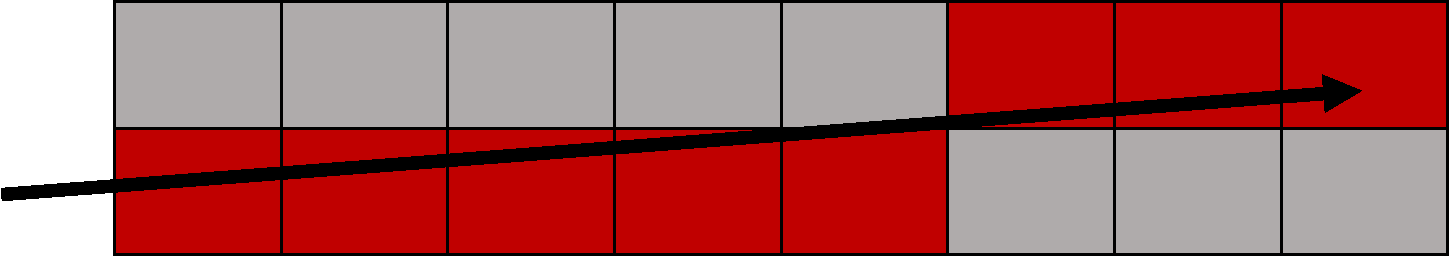
\includegraphics[width=\textwidth]{monte_carlo/delta_tracking/figures/tally_ray.pdf}
  \caption{A particle tallying to multiple tally mesh bins (shown in red). Implemented as a single operation for both surface and Woodcock-delta tracking in MC/DC.}
  \label{fig:tally_ray}
\end{figure}

MC/DC v0.11.1 \cite{morgan_monte_2024} has an optimized tally algorithm where track-lengths to multiple structured mesh cells (which we call voxels
\footnote{\textit{voxel} is the 3D analog to a pixel, here we mean it as a cube mesh bin to tally into}
)are scored in a single operation.
This algorithm is based on a sweeping method where the initial state (mesh cell index, exact ($x$, $y$, $z$) position, direction of travel, speed, and particle clock) are known, as is the distance to the next event.
The particle is then swept from voxel to voxel, tallying the exact track-length traveled in a given voxel along the way.
Figure \ref{fig:tally_ray} shows a hypothetical particle track and the mesh bins to be tallied to (in red) in a single operation.
In MC/DC's normal algorithm this is done even before moving a particle to an event while surface tracking.

In this work, we used this voxlized tally scheme when undergoing Woodcock-delta tracking.
Even if a particle collision is rejected that particle still physically moved to the location that was sampled, allowing the use of the track-length estimator.
In this scheme the distance tallied is always the distance sampled with the majorant, baring census crossings or distance to boundary events.

To verify that MC/DC's voxelized track tallies with delta tracking both converges to the correct solution and at the correct rate we use four anaclitic based benchmark problems.
We compare the error from integral quantities of interest to a reference solution then plot the error as a function of increasing particle count.
The convergence rate should be the standard Monte Carlo convergence rate of $N^{-1/2}$.
Our verification problems are
\begin{itemize}
    \item AZURV1 time dependent benchmark both super and sub critical (figure \ref{fig:azurv1}) \cite{ganapol_homogeneous_2001};
    \item A time dependent infinite pin cell using the 371 group SHEM cross sections (figure \ref{fig:shem}) \cite{hfaiedh_2005_shem}; and 
    \item Reed's Problem (figure \ref{fig:reeds}) \cite{reed_difference_1971};
    \item A purely absorbing slab (figure \ref{fig:abs_slab}).
\end{itemize}
\begin{figure}
  \centering
  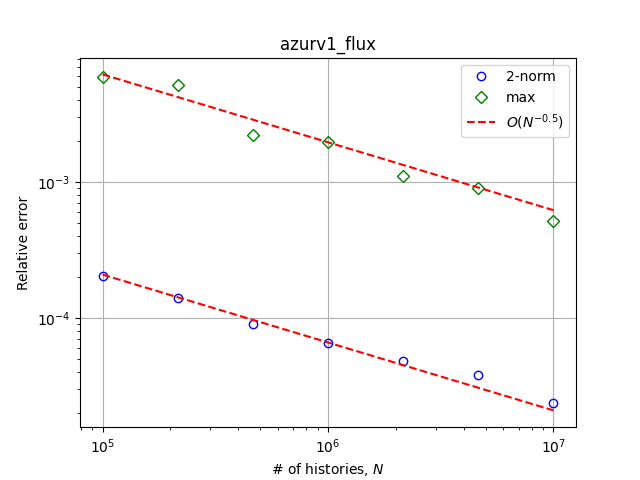
\includegraphics[width=0.32\linewidth]{monte_carlo/delta_tracking/figures/verification/azurv1/azurv1_flux.png}
  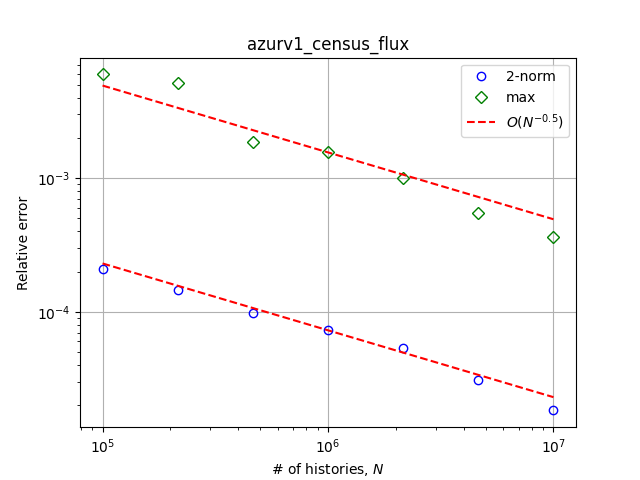
\includegraphics[width=0.32\linewidth]{monte_carlo/delta_tracking/figures/verification/azurv1/azurv1_census_flux.png}
  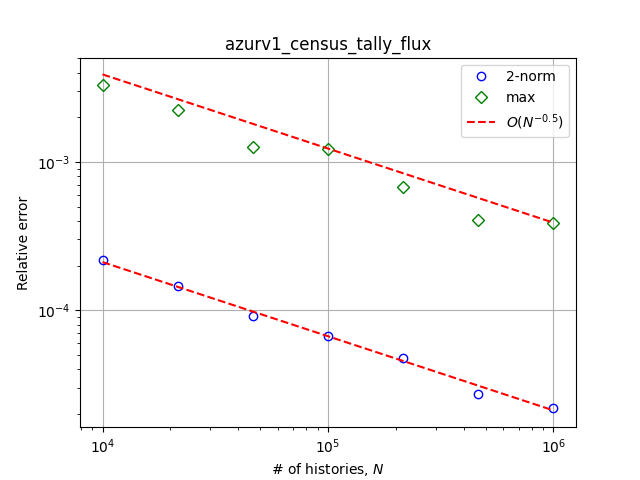
\includegraphics[width=0.32\linewidth]{monte_carlo/delta_tracking/figures/verification/azurv1/azurv1_census_tally_flux.png}
  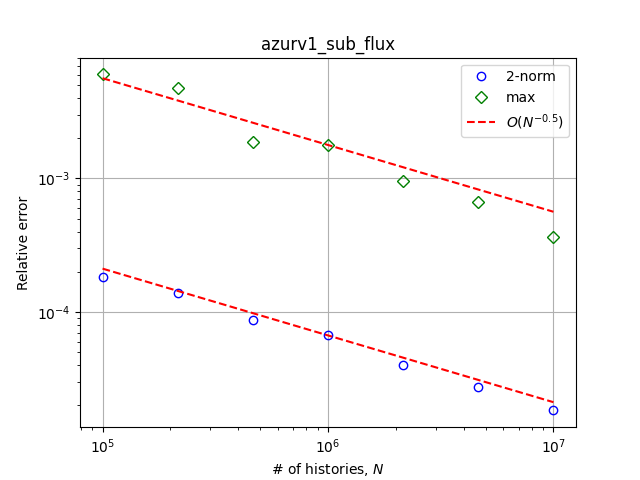
\includegraphics[width=0.32\linewidth]{monte_carlo/delta_tracking/figures/verification/azurv1/azurv1_sub_flux.png}
  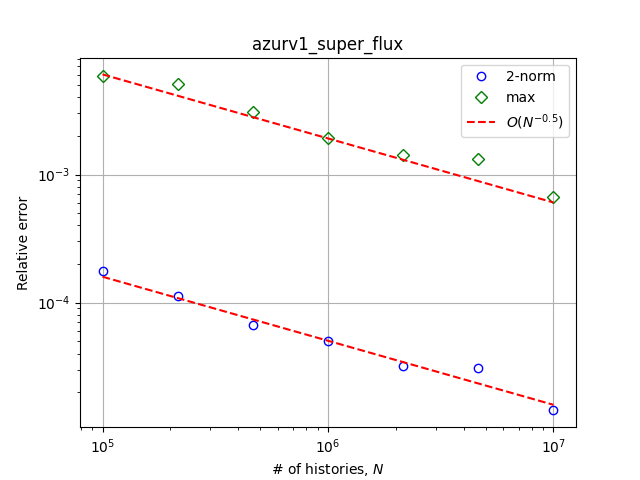
\includegraphics[width=0.32\linewidth]{monte_carlo/delta_tracking/figures/verification/azurv1/azurv1_super_flux.png}
  \caption{Convergence rate verification of AZURV1 \cite{ganapol_homogeneous_2001} }
  \label{fig:azurv1}
\end{figure}
\begin{figure}
  \centering
  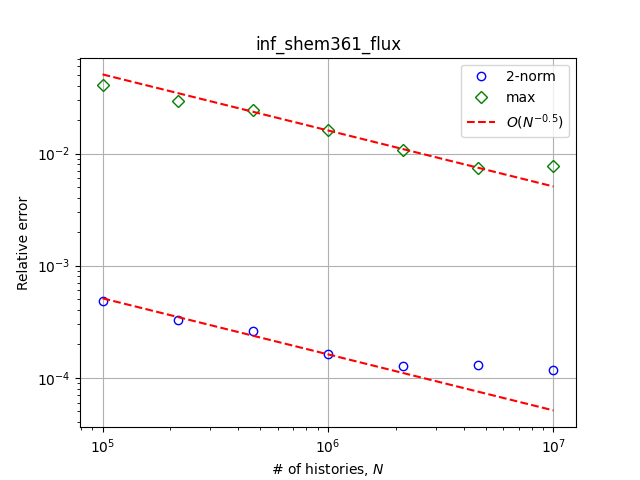
\includegraphics[width=0.32\linewidth]{monte_carlo/delta_tracking/figures/verification/shem/inf_shem361_flux.png}
  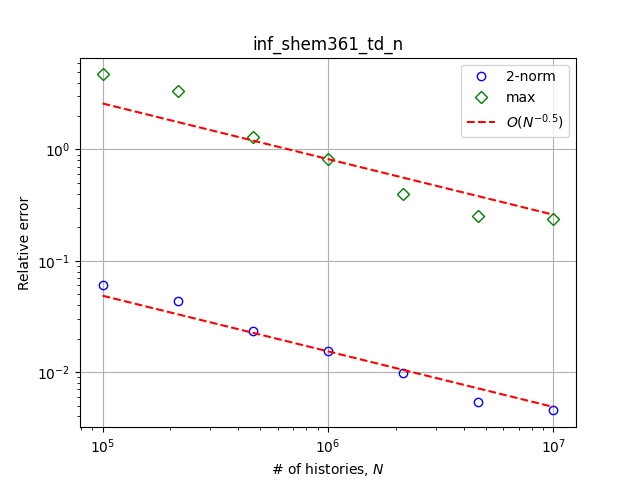
\includegraphics[width=0.32\linewidth]{monte_carlo/delta_tracking/figures/verification/shem/inf_shem361_td_n.png}
  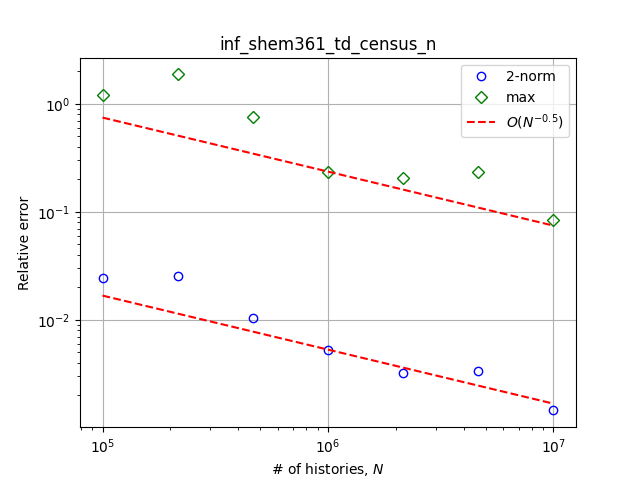
\includegraphics[width=0.32\linewidth]{monte_carlo/delta_tracking/figures/verification/shem/inf_shem361_td_census_n.png}
  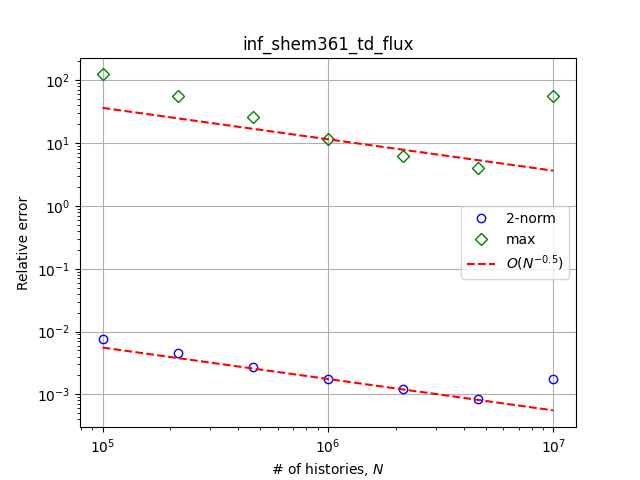
\includegraphics[width=0.32\linewidth]{monte_carlo/delta_tracking/figures/verification/shem/inf_shem361_td_flux.png}
  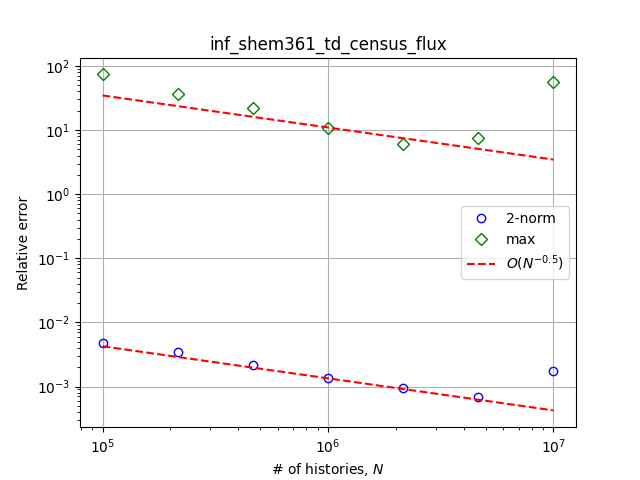
\includegraphics[width=0.32\linewidth]{monte_carlo/delta_tracking/figures/verification/shem/inf_shem361_td_census_flux.png}
  \caption{Convergence rate of an infinite pin using the SHEM 361 group cross section library \cite{hfaiedh_2005_shem}}
  \label{fig:shem}
\end{figure}
\begin{figure}
  \centering
  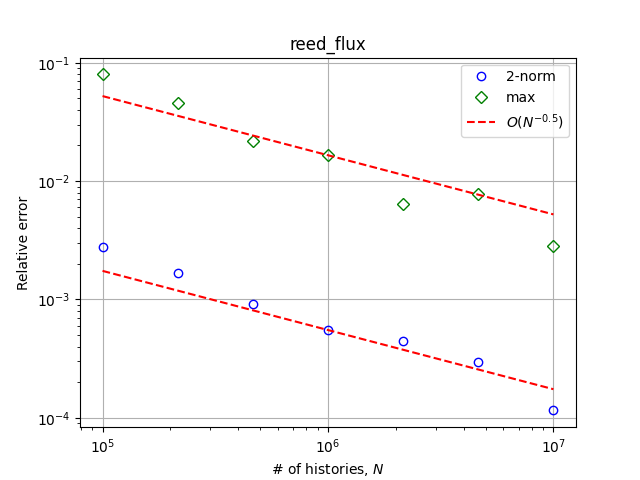
\includegraphics[scale=0.75]{monte_carlo/delta_tracking/figures/verification/reed/reed_flux.png}
  \caption{Convergence rate of flux from Reed's problem \cite{reed_difference_1971}}
  \label{fig:reeds}
\end{figure}
\begin{figure}
    \centering
    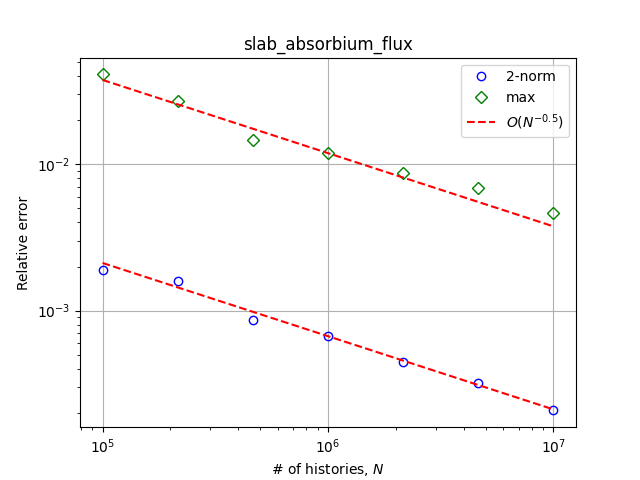
\includegraphics[width=0.75\linewidth]{monte_carlo/delta_tracking/figures/verification/abs_slab/slab_absorbium_flux.png}
    \caption{Convergence rate of QOIs for a purely absorbing slab wall problem}
    \label{fig:abs_slab}
\end{figure}

All verification simulations show the $N^{-1/2}$ convergence rate expected for Monte Carlo results.
This verifies that we are getting the expected results with voxelized Woodcock-delta tracking.


\subsection{Hybrid-In-Material}
\label{sec:material_exc}


The first hybrid method we implement in MC/DC is a material or region based decision on weather to us surface or delta tracking we call ``hybrid-in-material".
Each particle is given an additional flag declaring which transport algorithm it is using to sample a distance to next event.
At the beginning of the \texttt{determine\_next\_event} function the tracking flag will be set to \texttt{true} if the particle is in a material region declared by the user to undergo delta tracking or \texttt{false} if in a region where delta tracking should not be used. 
This is similar to in Serpent2's algorithm however our voxelized tally structure allows us to use track-length estimators in all regions not just those undergoing surface tracking.
Also Serpent2's algorithm makes automatic decisions about where to surface and delta track based off a user supplied cut off value \cite{leppanen_development_2013} whereas we leave it as user option for now.


\begin{figure}
    \centering
    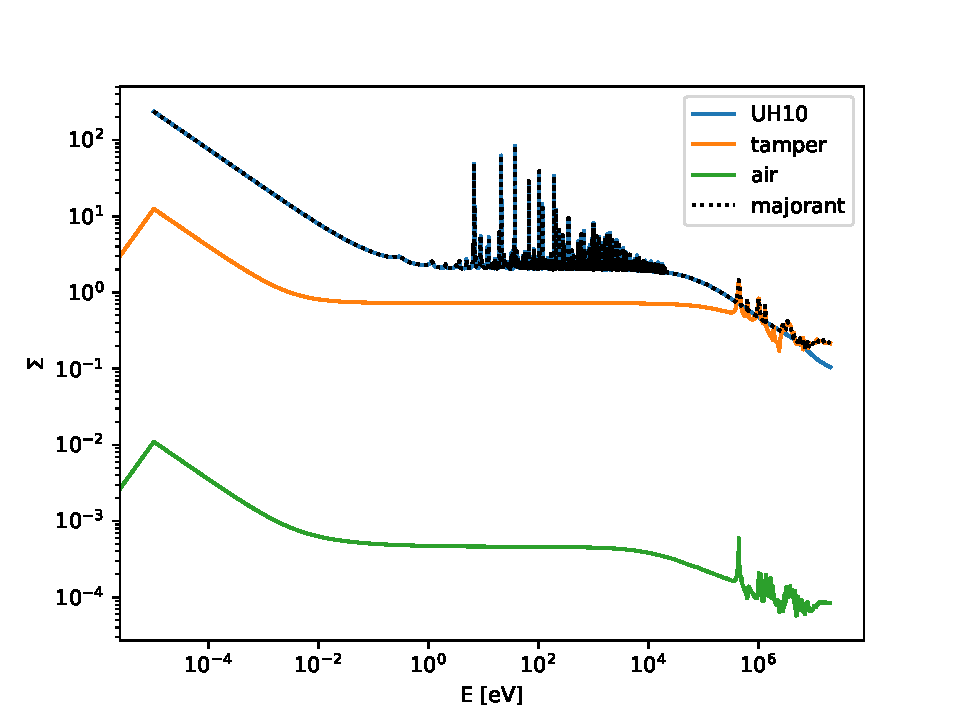
\includegraphics[width=0.75\textwidth]{monte_carlo/delta_tracking/figures/macro_majorant_dragon.pdf}
    \caption{Continuous energy macroscopic majorant cross-section ($\maj$) for the Dragon burst problem.}
    \label{fig:majorant_dragon}
\end{figure}

Conventional wisdom dictates that delta tracking should not be used in systems with strong localized absorbers as the majorant will be governed by cross sections much larger then others in the system.
Figure \ref{fig:majorant_dragon} shows the cross section information for the Dragon burst problem we describe in section \ref{sec:benchmarks}.
Conventional wisdom would suggest that this is a simulation that does not warrant Woodcock-delta tracking.
This simulation contains three materials, two of which (the fuel and tamper) have similar cross sections over all energies clumped together.
However the cross sections modeling air are over four orders of magnitude under cross sections describing the fuel and tamper.
This means in the air, particles will get stuck in the rejection sampling loop having phantom collision after phantom collision and statistically rarely complete a particle history.
Furthermore for classical delta tracking (where only a collision estimator can be used) the tallies in the air will be highly variant as there will be statistically few collisions taking place.
Using surface tracking in the air and delta tracking in the material may give a performance boost in this problem.

\subsection{Hybrid-In-Energy}
\label{sec:cutoff}

The second hybrid method we call ``hybrid-in-energy", and is a decision to do delta tracking above a given user-defined energy and conduct surface tracking below.
For neutrons, high energies (or speeds) are characterized by relatively long mean free paths (small cross sections) as they are physically going too fast to interact with anything.
Delta tracking generally does better under these conditions compared to surface tracking as surface tracking would get stuck moving particles from region to region whereas delta tracking can stream particles through the whole problem.
Furthermore at higher energies in many systems the majorant will more closely match the cross sections of materials in alleviating issues with the rejection sampling loop.

For example consider a continuous energy version of the C5G7 benchmark reactor geometry \cite{jia_hou_oecdnea_2017}.
The material composition is given by table \ref{tab:c5ce} in appendix \ref{app:c5ce_mat}.
Figure \ref{fig:majorant_c5ce} shows the macroscopic material cross-sections for the 7 material reactor with the majorant in black.
Around \SI{10}{\kilo\electronvolt} the neutron resonances end and the problem can be considered high energy.

If using delta tracking for this whole problem neutrons will get stuck in resonance frequencies where the rejection sampling loop will be called too much degrading the performance of delta tracking.
Therefore it would be ideal to delta track above \SI{50}{\kilo\electronvolt} (as to completely avoid neutron resonances) and surface track under that threshold.

\subsection{Implementation in MC/DC}
\label{sec:implementation}

Monte Carlo Dynamic Code is purpose built to implement and test time dependent Monte Carlo novel numerical methods at scale \cite{morgan_2025_monte}.
It uses a novel for the field development structure where Python scripted compute kernels are compiled via the Numba compiler to run on CPUs and with the Harmonize GPU runtime manager to run on GPUs.

MC/DC allowed us to rapidly experiment with these methods at scale on both CPUs and GPUs on time dependent problems of interest.
Delta tracking methods can be easy to implement in a code that already conducts surface tracking. 
Generally to implement delta tracking in a code that already implements surface tracking add are:
\begin{enumerate}
    \item Pre-process functions to generate a majorant (MC/DC's implementation is in \ref{app:majorant});
    \item \texttt{if} statements in \texttt{distance\_to\_next\_event} functions to compute relevant distances;
    \item Functions to implement boundary conditions when in delta tracking mode; and
    \item Elevate delta tracking options to the input deck.
\end{enumerate}
Our implementation added about \num{450} lines of code, of which half was to produce various types of majorants (an example can be found in \ref{app:majorant}). 
Only about \num{200} lines of code where required in the compute kernels themselves to implement delta tracking in MC/DC.
This process was similar to implementing hybrid surface-delta tracking methods in MCATK \cite{morgan2023delta}.
This is also similar to current ongoing work in OpenMC.

We found the most complicated issue when implementing delta tracking in MC/DC to be the boundary conditions.
Surface tracking codes (like MC/DC) often enforce boundary conditions as a surface options, something to avoid when delta tracking.
Vacuum boundary conditions are simple as if or when a particle is determined to be out of the problem when looking for a cross section in the rejection sample particles are killed.
For reflecting surfaces we use a stripped down version of \texttt{distance\_to\_nearest\_surface} function in MCDC to compute distances to reflecting surfaces, if any.
Many reflecting boundary conditions including the ones we implement in our benchmark problems are imposed on planar surfaces, making the distance to boundary computation cheap.
In effect we are still surface tracking only to our reflecting boundary surfaces.


\section{Verification of Woodcock-Delta Tracking with Continuously Moving Surfaces}

To verify that Woodcock-delta tracking can be used in conjunction with the continuously moving surfaces in MC/DC we use the moving pellet regression test from MC/DC's test suite \cite{morgan_monte_2024}.
In it a rectangular fuel element which moves through a region with a small source.
As the pellet moves closer and farther from the source region the fission rate in the pellet changes.
Figure \ref{fig:moving_pellet} at left shows the fission reaction rate density at various points in time.
The outline of the pellet can be seen clearly.
These plots where produced using Woodcock delta tracking with a collision estimator and matched plots produced when using surface tracking with a collision estimator.

\begin{figure}
    \centering
    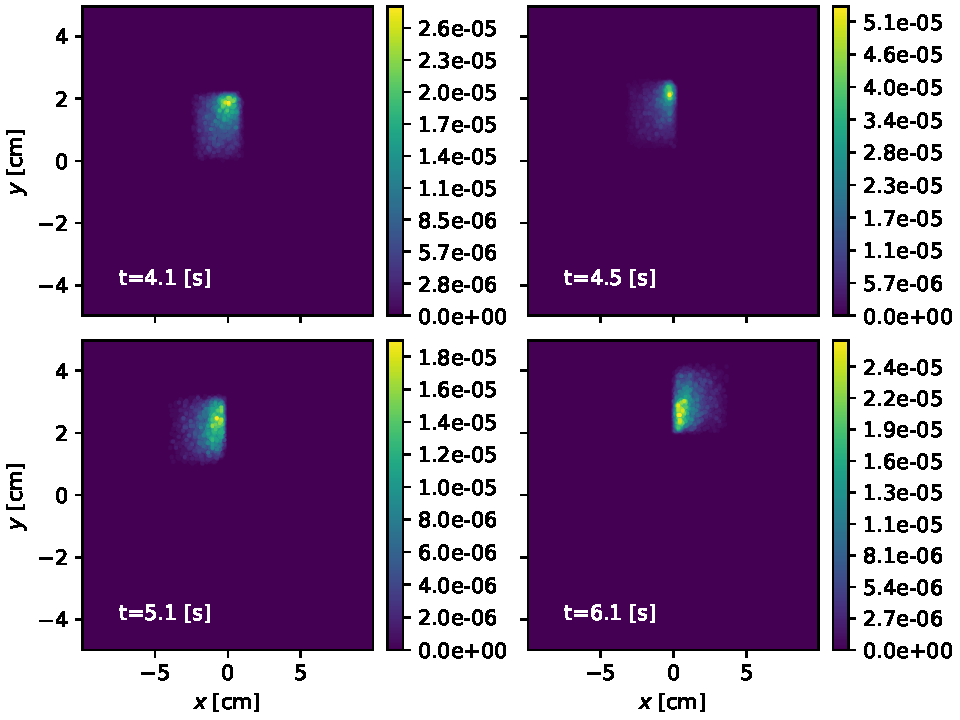
\includegraphics[width=0.49\linewidth]{monte_carlo/delta_tracking/figures/verification/moving_pellet_plot.pdf}
    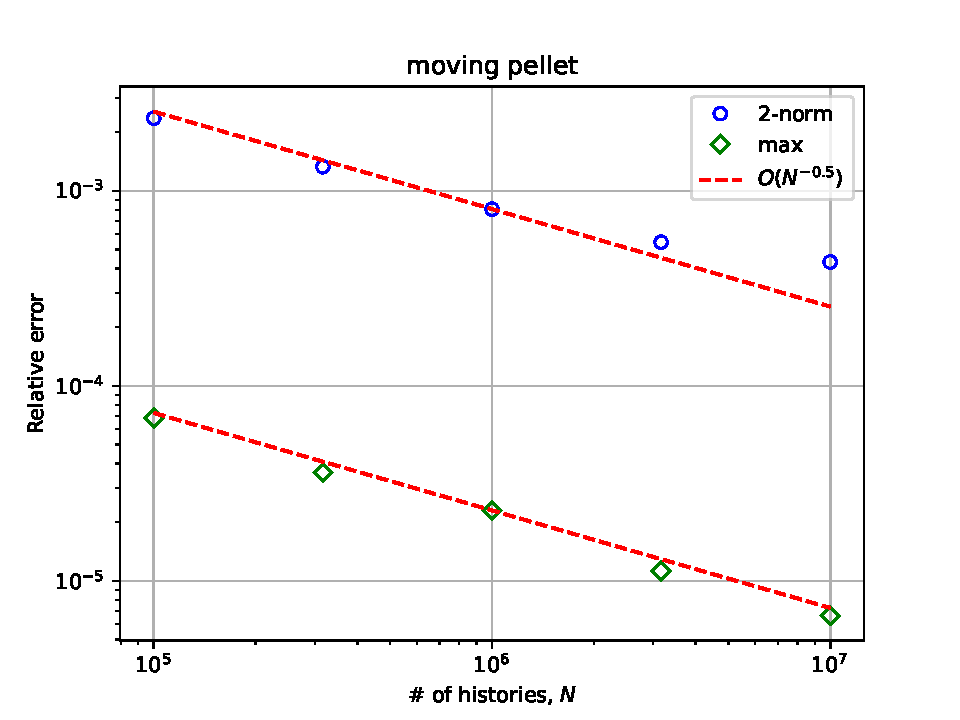
\includegraphics[width=0.49\linewidth]{monte_carlo/delta_tracking/figures/verification/moving_pellet.pdf}
    \caption{(left) Fission flux density at various points in time for the moving pellet problem, using Woodcock-delta tracking with a collision estimator (right) convergence between fluxes produced from surface and Woodcock-delta tracking both with the track-length estimator, showing $N^{-1/2}$ convergence rate.}
    \label{fig:moving_pellet}
\end{figure}

To further verify Woodcock delta tracking with continuous movement physics we regressively compare the flux solutions provided from traditional surface tracking and delta tracking with voxelized tallies at various particle counts.
We compute 
\begin{equation}
    \epsilon_N = |\phi_N^{\text{surface}} - \phi_N^{\text{delta}} |_2
\end{equation}
at every choice of $N$ particles.
We then compare the error of flux over particles to ensure the expected Monte Carlo convergence rate ($N^{-0.5}$).
Figure \ref{fig:moving_pellet} at right shows the error converging at the expected rate.
This regressively verifies that Woodcock-delta tracking can be used in conjunction with continuously moving surfaces.
We also produced this same plot for both tracking method using a collision estimator for both flux and fission tallies all of which matched the expect Monte Carlo convergence rate.

\section{Benchmark Problems}
\label{sec:benchmarks}

% vairiance reudciton and figure of merrit
The performance of a given Monte Carlo algorithm for a specified problem is a function of solver variance ($\sigma^2$, from the Monte Carlo process itself) and wall-clock runtime it takes to get that solution.
If a certain algorithm can forum a solution with low variance at fewer particles it may still yet be not considered as suitable as an algorithm that takes many many more particles to reach that statistical variance if it is too slow.
So a measurement must be used to take into account both the variance of a given solution and Figure of Merit (FOM) is one such measure. In this work we will use 
\begin{equation}
    FOM = \frac{1}{\hat{\sigma}^2 t_{wc}}
\end{equation}
where $\hat{\sigma}^2$ is the L$_{1}$ norm (over phase space) of the variance of the solution provided by the Monte Carlo solver and $t_{wc}$ is the wall clock runtime required to obtain that solution.

\begin{figure}
    \centering
    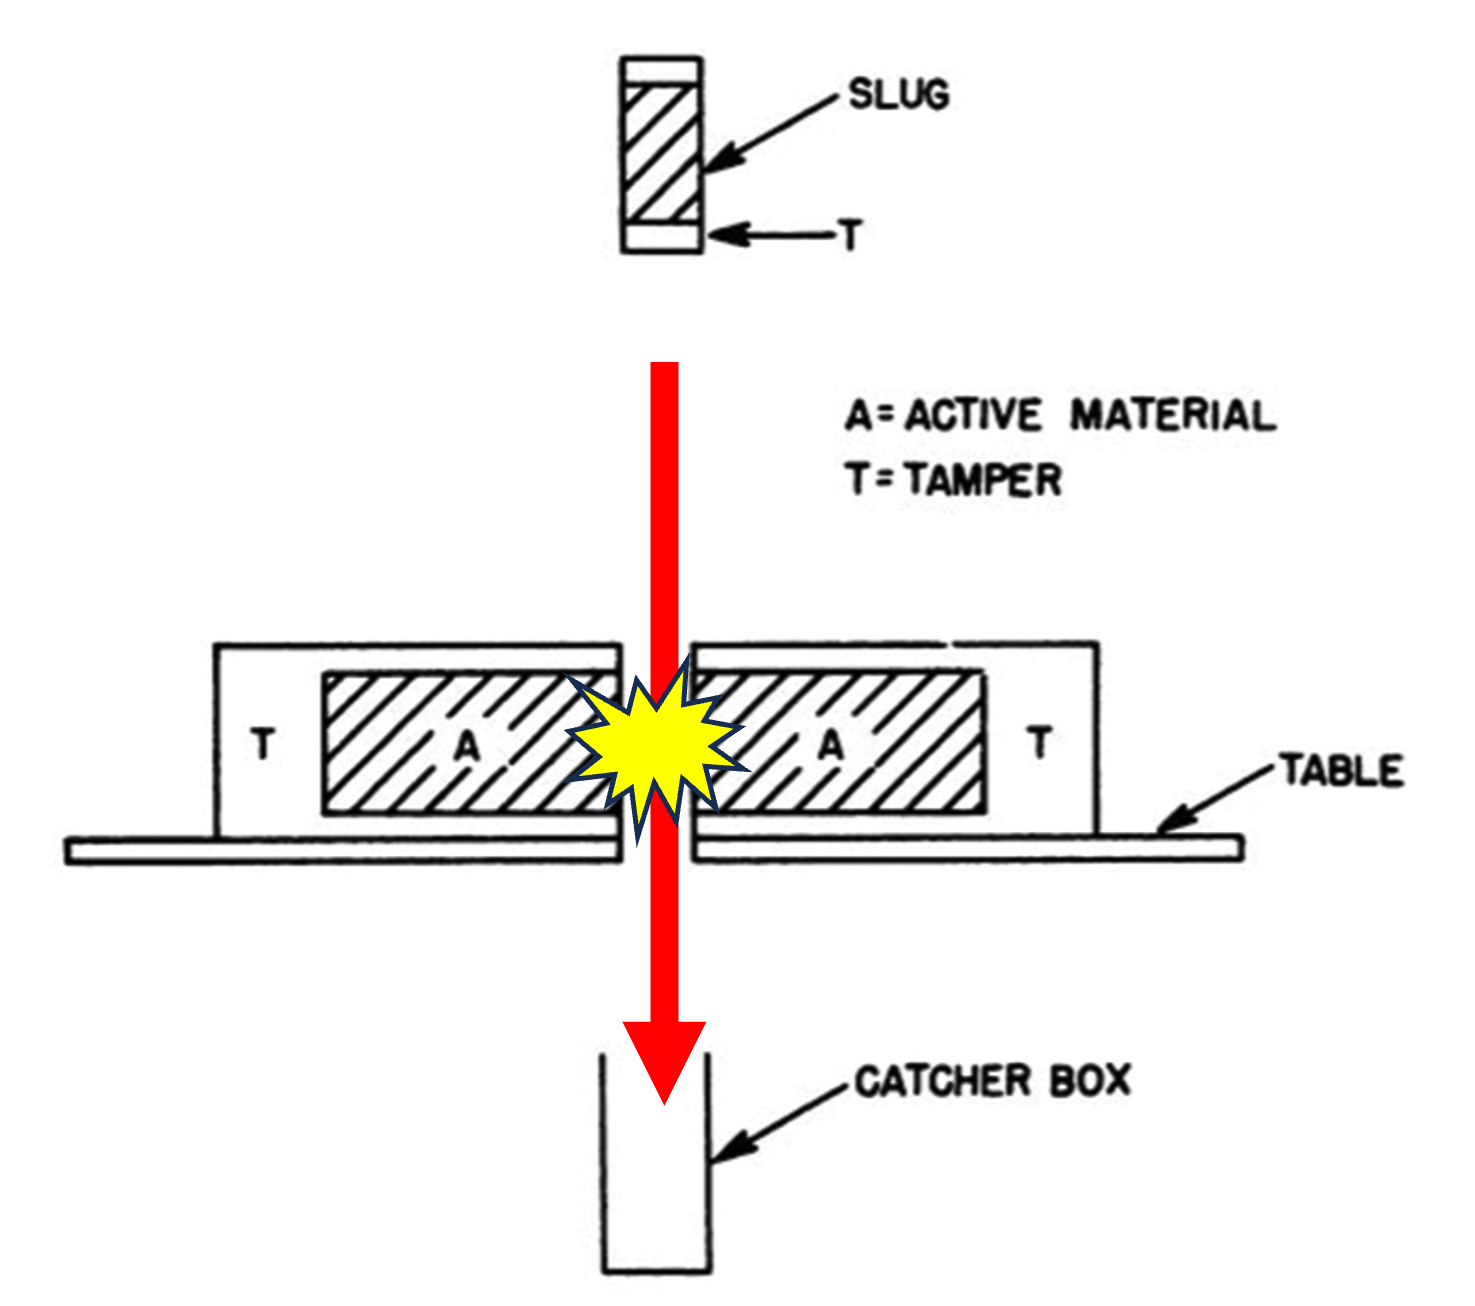
\includegraphics[width=0.48\linewidth]{monte_carlo/delta_tracking/figures/dragon.png}
    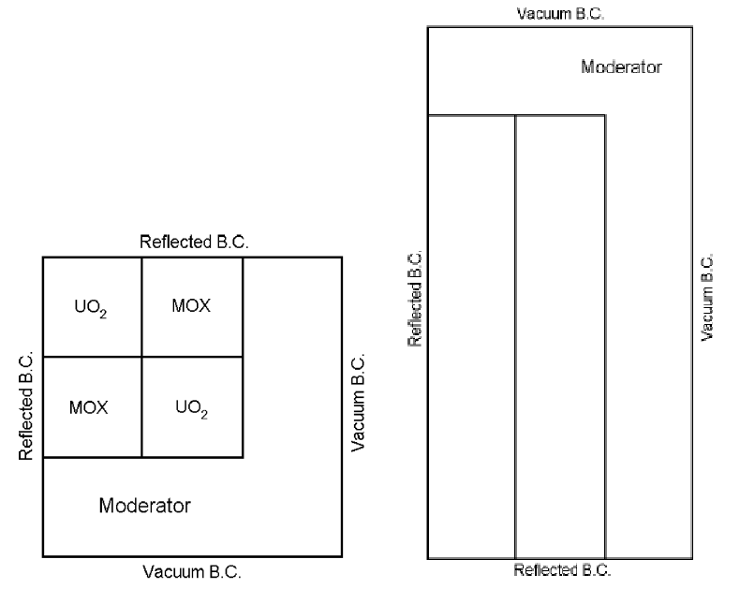
\includegraphics[width=0.48\linewidth]{monte_carlo/delta_tracking/figures/c5g7.png}
    \caption{Schematics (left) Dragon burst problem \cite{kimpland2021dragon} (right) C5G7 reactor quarter (via reflecting boundaries) \cite{jia_hou_oecdnea_2017}}
    \label{fig:schems}
\end{figure}

% the problems we run themselves
We use four fully time dependent fixed source benchmark problems to compare the voxlized tally scheme and hybrid methods proposed in this work to surface tracking on CPU and GPU machines.
Two are multi-group, two are continuous energy.
Table \ref{table:benchmark_problems} summarizes the size (in both mesh and particle count) of each benchmark problem.
Some problems may not be suited for delta tracking methods but are used anyway here to show both correctness under physical problem dynamics (i.e., moving surface) and demonstrate algorithmic improvement in under highly exaggerated problem parameters.

\begin{table}[htb]
  \centering
  \begin{tabular}{@{}l c c c @{}} \toprule
    Problem & $N_{mesh}$ & $N_{particles}$ & Energy physics \\ \midrule
    Kobyashi & \num{120e3} & \num{1e10} & MG (1 group) \\
    Dragon Burst & \num{4.0e6} & \num{3e9} & Cont. E (3 materials) \\
    C5G7 & \num{3.9e6} & \num{1e7} & MG (7 groups) \\
    C5CE & \num{544e3} & \num{1e5} & Cont. E (7 materials) \\
    \bottomrule
  \end{tabular}
  \caption{Time dependent benchmark problems.} 
  \label{table:benchmark_problems} 
\end{table}

% koby intro
The first benchmark we consider is the time dependent version of the Kobyashi problem \cite{Kobayashi2001} introduced by \cite{morgan_2025_monte}.
We run this problem with 10 batches with \num{1e9} particles per batch (\num{1e10} particles total) with traditional surface tracking, traditional delta tracking with a collision estimator, and a delta tracking using the voxelized tally method.
This problem contains two materials, a dense region (characterizing a solid), and a low density region modeled by air (characterizing a void) in a single energy group.
There are a 120k structured tally mesh cells in the $x$-$y$ plane and in time.

% acident intro
Figure \ref{fig:schems} at right shows the geometry for the next two simulations we consider based on the C5G7 benchmark problem \cite{jia_hou_oecdnea_2017}.
We model a 4 phase accident where-in a pressurized light water reactor reactor is powering up by removing control rods.
Figure \ref{fig:c5g7} at left shows the normalized flux density as a function of time (produced from reactor point kinetics) and the four phases shaded as gray, green, red, and blue.
Phase one (shaded gray) starts with the reactor operating at steady state.
In phase two (shaded green) the control rods are removed from the reactor to power up to a new steady state.
Phase three (shaded red) begins when a bank of control rods gets stuck in the fully withdrawn position.
Towards the end of phase three the reactor sees a rapid spike in power that ends when at \SI{15}{\s} all the control rods are forced into the reactor ending the accident.
The fourth and final phase sees the reactor decaying in power as the delayed neutron population dies out.
Figure \ref{fig:c5g7} shows plots of flux in the $x$-$y$ plan at various points in time including at \SI{14.95}{\s} the maximum power excursion.
These results are produced from running \num{1e6} particles in \num{10} batches (total of \num{1e7} particles).

\begin{figure}
    \centering
    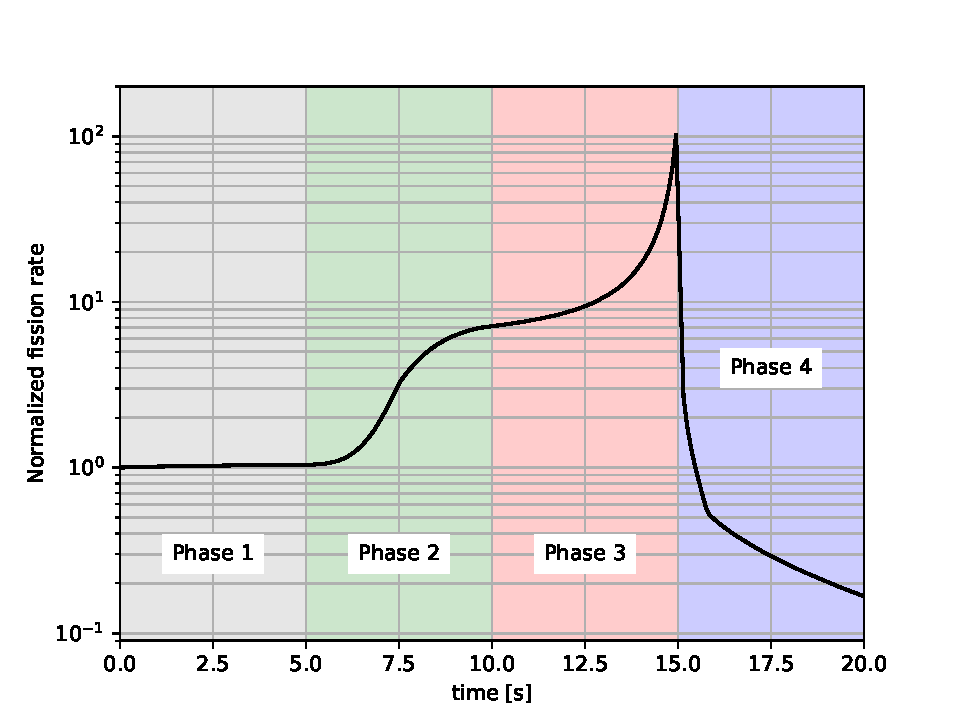
\includegraphics[width=0.48\linewidth]{monte_carlo/delta_tracking/figures/c5/acc.pdf}
    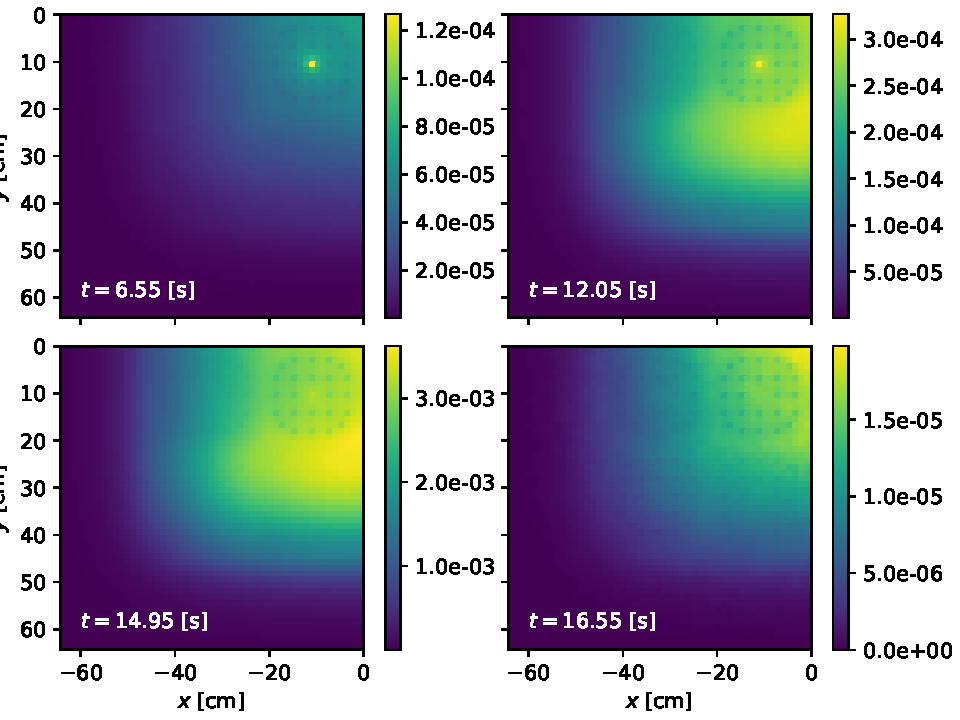
\includegraphics[width=0.48\linewidth]{monte_carlo/delta_tracking/figures/c5/flux.pdf}
    \caption{C5G7 stuck rod accident simulation, (left) flux densities through time, (right) scalar flux on x-y plane (top view) at points in time}
    \label{fig:c5g7}
\end{figure}

We first model this problem using the 7 group materials described by the normal C5G7 benchmark \cite{jia_hou_oecdnea_2017} which we will call C5G7 in the remainder of this work.
We model C5G7 with \num{3.9} million mesh cells in a full 3D, time and energy dependent tally mesh.
The movement of the control rods into and out of the reactor is controlled with MC/DC's continuous movement functionality.
To verify that the delta tracking methods we explore converge to the correct solutions while in transport with continuously moving surfaces we compare delta tracking solutions to solutions provided by surface tracking (which has already been verified and validated).
Performance data is collected by running \num{1e6} particles in \num{10} batches (total of \num{1e7} particles).

Next we define a continuous energy version of the C5G7 geometry we call C5CE undergoing the same 4-phase accident.
Table \ref{tab:c5ce} in appendix \ref{app:c5ce_mat} shows material compositions for the C5CE problem.
Using this benchmark we evaluate both the voxelized tally method as well as the hybrid-in-energy method described in section \ref{sec:cutoff}.
Figure \ref{fig:majorant_c5ce} at right plots the macroscopic total and majorant cross sections over energy for the materials in C5CE.
The neutron resonances end around \SI{10}{\kilo\electronvolt} so we set a cut off at \SI{50}{\kilo\electronvolt}.
When running this problem particles moving at speeds above \SI{50}{\kilo\electronvolt} MC/DC will use voxelized Woodcock-delta tracking and blow it will use traditional surface tracking.
We expect this to provide significant speedup over all previous methods explored in this problem as we avoid both down falls of either tracking method (surface tracking moving from surface to surface and delta tracking getting stuck in the rejection sample). 
To quote Miley Cyrus, ``you get the best of both worlds" \cite{cyrus_best_2005}.
C5CE also includes the same continuously moving surfaces as C5G7 so it serves as an additional verification that delta tracking methods can be used in conjunction continuously moving surfaces.
We model this problem with \num{447} mesh tally bins in 2D $x$-$y$ geometry (integrated along $z$) time and energy dependent tally mesh.
We run \num{1e5} particles in a single batch.

% dragon intro
The next problem we consider is a full time dependent simulation of the historical Dragon-burst experiments \cite{kimpland2021dragon}.
It was conducted in 1944 during the Manhattan project to prove that criticality could be achieved with prompt neutrons only.
Previous experiments, like the Chicago Pile One, used delayed neutrons to achieve criticality.
Figure \ref{fig:schems} at left shows a schematic of the experiment where a slug of highly enriched (75\%) Uranium Hydride ($UH_{10}$) was doped through a core with additional fuel.
As the slug moved through the core a prompt critical reaction was triggered as critical mass was achieved.
Before the super critical burst could become a problem (i.e. a deadly uncontrollable blast), gravity would pull the slug out of the core, ending the reaction.
Kimpland et. al showed that this burst criticality experiment could achieve over 9 orders of burst magnitude \cite{kimpland2021dragon}.
Work is on going to model the problem up to 9 orders of burst magnitude in MC/DC but here we use a less reactive version (25\% enrichment) to verify delta tracking with the hybrid-in-material method described in section \ref{sec:material_exc} and additional verification for delta tracking with continuously moving surfaces.
Figure \ref{fig:dragon_results} shows the overall flux density through time at left and a y-z plot of scalar flux at various points in time on the right.

\begin{figure}
    \centering
    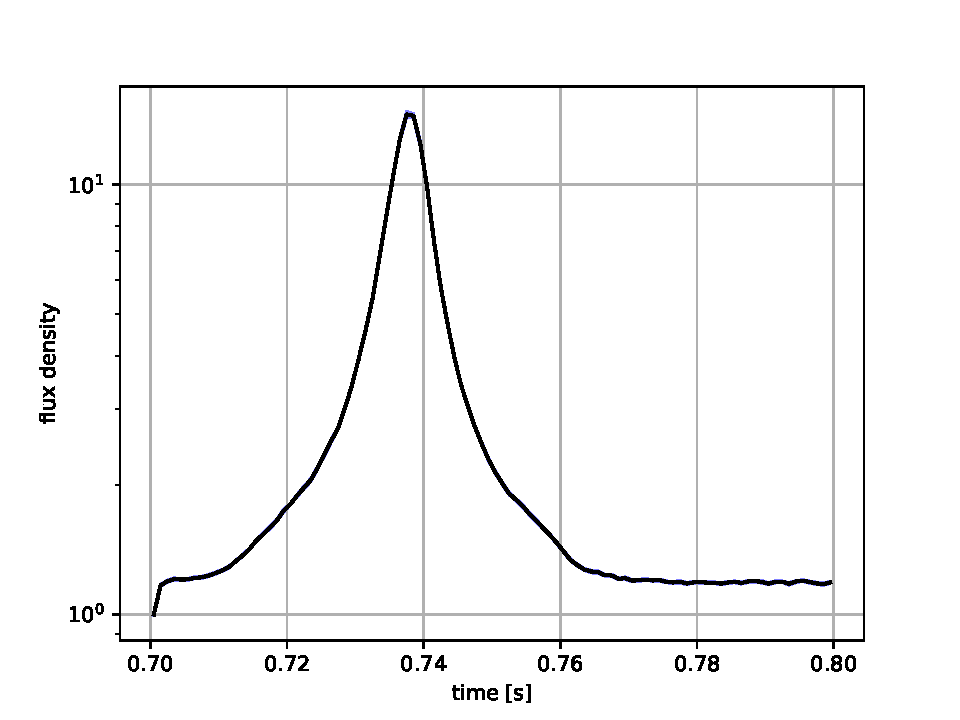
\includegraphics[width=0.48\linewidth]{monte_carlo/delta_tracking/figures/dragon/dragon_curve.pdf}
    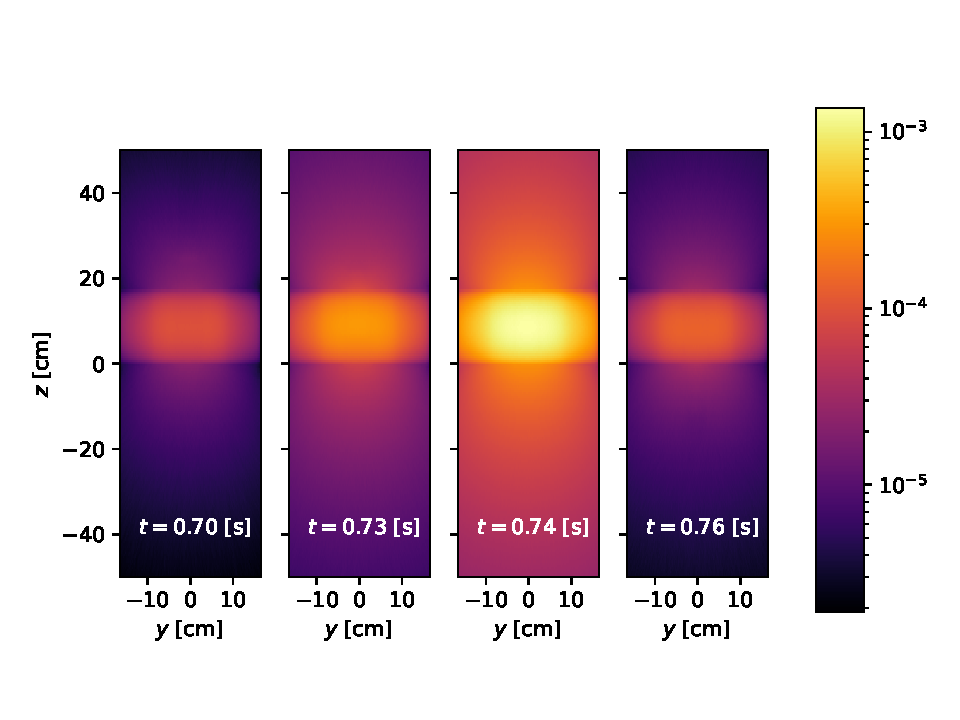
\includegraphics[width=0.48\linewidth]{monte_carlo/delta_tracking/figures/dragon/flux_dragon.pdf}
    \caption{Dragon burst simulation, (left) flux density through time, (right) scalar flux on y-z plane (side view) at points in time.}
    \label{fig:dragon_results}
\end{figure}

Figure \ref{fig:majorant_dragon} at left shows the continuous energy macroscopic total cross sections in the model we simulate.
The majorant, tamper and fuel cross sections all sit almost 4 orders magnitude above the cross section for air.
This is due to air being low density meaning fewer atoms for neutrons to interact with.
We expect any delta tracking algorithm to perform quite poorly in this model for a number of reasons.
First when undergoing delta tracking particles in the air region will get stuck in the rejection sample loop for a long time as the majorant is orders of magnitude larger and will sample very small distance before conducting a rejection sample.
Second as much of the problem is a void region the collision estimator that normal delta tracking requires will provide poor tallies in those regions
Third the problem is geometrically simple: consisting of a rectangular slug moving through a rectangular slab with a complimentary hole.
Traditional wisdom suggests that delta tracking performs best in complex materials.
The point of comparing delta tracking methods for this specific problem is to first confirm that delta tracking works with such a dynamic problem (the slug is modeled using MC/DC's continues movement functionality) and if we measure superior performance to standard delta tracking when using the hybrid-in-material method.

\section{Results}

% TLEase add the following required packages to your document preamble:
% \usepackage{multirow}
\begin{table}
\centering
\begin{tabular}{llllll}
\hline
Problem & Tracking Alg. & Estimator & Runtime [s] & $|\hat{\sigma}^2|_1$ & FOM \\ \hline
\multirow{4}{*}{Kobyashi}
 & surface  & TLE & \num{1574} & \num{4.514e-3} & 0.1407 \\
 & surface  & CE & \num{1014} & \num{9.552e-2} & 0.0103 \\
 & delta  & TLE & \num{1298} & \num{4.539e-3} & 0.1697 \\ 
 & delta  & CE & \num{817.2} & \num{2.062e-1}  & 0.0059 \\
 \hline
 

 
\multirow{4}{*}{C5G7}
 & surface  & TLE & \num{7926} & \num{1.295e-4} & \num{0.9744} \\
 & surface  & CE & \num{3173} & \num{1.295e-4} & \num{2.4336} \\
 & delta  & TLE & \num{2870.} & \num{1.400e-4} & \num{2.4889} \\
 & delta  & CE & \num{1820} & \num{2.15e-4} & \num{2.5515} \\
 \hline

 
\multirow{6}{*}{C5CE} 
 & surface  & TLE & \num{734.6} & \num{1.812e-3} & \num{0.7484}\\
 & surface  & CE & \num{587.8} & \num{1.812e-2} & \num{0.9391}\\
 & delta  & TLE & \num{496.8} & \num{4.906e-3} & \num{0.4103} \\
 & delta  & CE & \num{555.0} & \num{1.173e-2} &  \num{0.1536} \\
 & hybrid-energy & TLE & \num{226.25} & \num{1.164e-3} & \num{3.798} \\ 
 & hybrid-energy & CE & \num{220.5} & \num{1.144e-3} & \num{3.965} \\ 
 \hline

 
\multirow{4}{*}{Dragon} 
 & surface  & TLE & \num{3816} & \num{1.163e-6} & \num{221.4} \\
 & delta  & CE & DNF$^*$ & - & - \\
 & delta  & TLE & DNF$^*$ & - & - \\
 & hybrid-in-material & TLE & \num{15493} & \num{1.106e-6} & \num{58.40} \\
 \hline
\end{tabular}
\caption{Results for benchmark problems on Dane (112$\times$ Intel Sapphire Rapids CPU cores). $^*$Did not finish in 8 hour time limit.}
\label{tab:dane_results}
\end{table}

%1.163327654958653e-06
%1.1056932706381267e-06

% Please add the following required packages to your document preamble:
% \usepackage{multirow}
\begin{table}
\centering
\begin{tabular}{llllll}
\hline
Problem & Tracking Alg. & Estimator & Runtime [s] & $|\hat{\sigma}^2|_1$ & FOM \\ \hline
\multirow{4}{*}{Kobyashi} 
 & surface  & TLE & \num{973.9} & \num{4.514e-3} & 0.2275 \\
 & surface  & CE & \num{840.6} & \num{9.952e-2} & 0.0125 \\
 & delta  & TLE & \num{831.8} & \num{4.539e-3} & 0.1697 \\ 
 & delta  & CE & \num{620.7} & \num{2.062e-1}  & 0.0078 \\
 \hline
 
\multirow{4}{*}{C5G7} 
 & surface  & TLE & \num{4598} & \num{1.305e-4} & \num{1.666} \\
 & surface  & CE & \num{2403} & \num{1.305e-4} & \num{3.1878} \\
 & delta  & TLE & \num{161} & \num{1.400e-4} & \num{4.4205} \\ 
 & delta  & CE & \num{789.3} & \num{2.152e-4} & \num{5.8860} \\

 \hline
 
\multirow{6}{*}{C5CE} 
 & surface  & TLE & \num{550.9} & \num{2.452e-3} & \num{0.7402}\\
 & surface  & CE & \num{465.9} & \num{2.452e-3} & \num{0.8753}\\
 & delta  & TLE & \num{500.7} & \num{1.690e-2} & \num{0.1182} \\
 & delta  & CE & \num{421.6} & \num{1.793e-2} &  \num{0.1323} \\
 & hybrid-energy & TLE & \num{291.7} & \num{1.557e-3} & \num{2.2023} \\ 
 & hybrid-energy & CE & \num{275.6} & \num{1.839e-3} & \num{1.9731} \\ 
 \hline
 
\multirow{4}{*}{Dragon} 
 & surface & TLE & \num{3993} & \num{1.163e-06} & \num{2153} \\
 & delta & CE & DNF$^*$ & - & - \\
 & delta & TLE & DNF$^*$ & - & - \\
 & hybrid-material & TLE & DNF$^*$ & - & - \\ \hline
\end{tabular}
\caption{Results for benchmark problems on Lassen (4$\times$ Nvidia Tesla V100). $^*$Did not finish in 8 hour time limit.}
\label{tab:lassen_results}
\end{table}

In this section we discuss performance results of the of the benchmarks described above with surface, traditional delta, voxelized delta tracking as well as the hybrid-in-energy and hybrid-in-material tracking algorithms.
In this section we also verify that the various delta tracking methods converge to the same solution as surface tracking while transporting on a geometry with continuously moving surfaces.

\subsection{Performance Results}

% testing systems
We ran our benchmark problems on high-performance computing systems available at Lawrence Livermore National Laboratory (LLNL): the Dane, and Lassen machines.
Dane is a CPU-only system with dual-socket Intel Xeon Sapphire Rapids CPUs, each with 56 cores for a total of 112 per node. 
Lassen is the open collaboration sibling to the Sierra machine with four Nvidia Tesla V100s GPUs and two IBM Power 9 CPUs per node.
We will make all performance statements against CPU runtime from a whole node of Dane (112 MPI threads, CPU) and a whole node of Lassen (4 MPI Threads, GPU).
We compile to Nvidia GPUs with CUDA v11.8 and
Nvida-PTX with Numba v0.59.0\footnote{Numba v0.59.1 is the most recent version to support Power9 CPUs}.
We compile to CPUs with Numba v0.60.0.
We build our delta tracking methods off of MC/DC v0.12.0 \cite{transport_cement_mcdc_2024} and compile with Harmonize v0.0.2 \cite{harmonize}.
We use double precision for all floating point operations.
% Introduce the table
Table \ref{tab:dane_results} and \ref{tab:lassen_results} show the wall-clock runtime, normalized standard deviations and figures of merit for our four benchmark problems from the Dane and Lassen machines respectively.

% Results Koby
The Kobyashi problem on Dane sees dramatic runtime improvements when moving from surface to delta tracking with a collision estimator.
However this does not make up for the two orders of magnitude additional variance on the tallies of interest.
This leads to a dramatically smaller figure of merit for traditional delta tracking (using a collision estimator) compared to surface tracking.
Figure \ref{fig:koby} shows the traditional delta tracking with a collision estimator on the bottom and our voxlized delta tracking on top at various points in time through the simulation.
It is clear to a casual observer that the collision estimator is producing a more variant (appearing as static-y or fuzzy) result than the track-length estimator.
Our voxlized tally method sees 21\% decrease in wall clock time compared with the same amount of normalized variance leading to a moderately improved figure of merit (\num{0.1697} and \num{0.1407} for our voxelized method and surface tracking respectively) 
This pattern of results, where traditional delta tracking is the fastest wall clock runtime with a normalized variance orders of magnitude above methods using a track-length estimator, will persist through the analysis of the other problems we consider.
As will the behavior of the voxelized delta method's runtime sitting between surface tracking and traditional delta tracking with similar variance to surface tracing results.


\begin{figure}
    \centering
    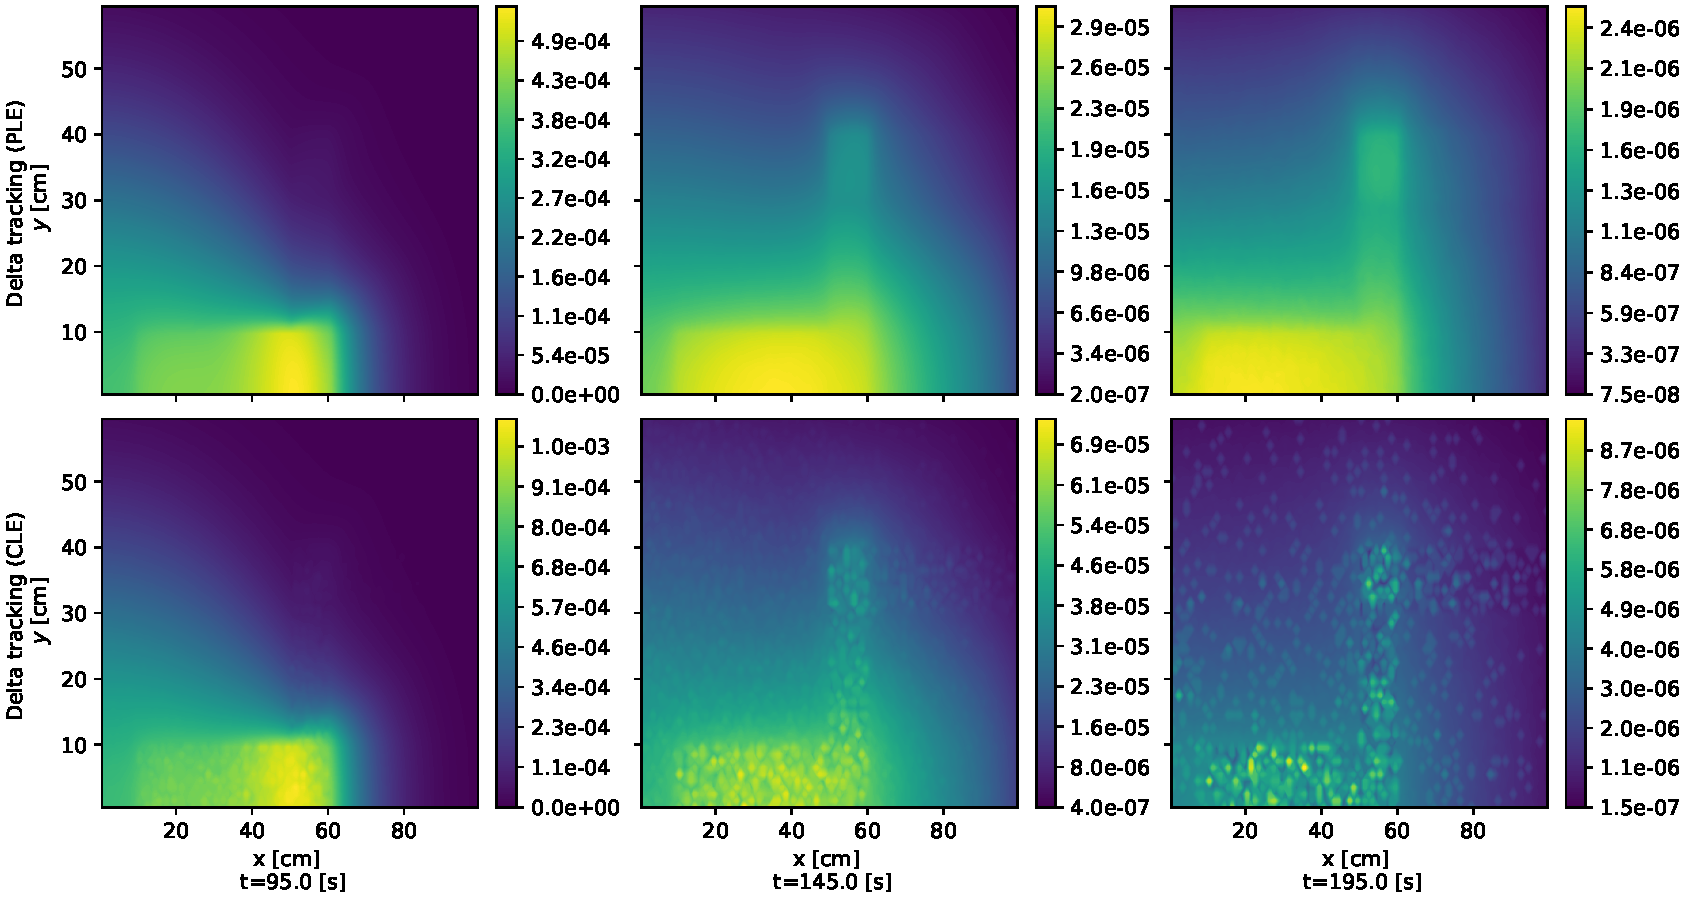
\includegraphics[width=\textwidth]{monte_carlo/delta_tracking/figures/cle_v_tle.pdf}
    \caption{Comparison of delta tracking using the track-length estimator (top row) and collision estimator (bottom row) at three points in time. Collision estimator has a much higher variance.}
    \label{fig:koby}
\end{figure}

% Restuls C5G7
Moving on to C5G7, the same pattern of results persists where traditional delta tracking sees the smallest wall-clock runtime with the highest variance (\SI{1673}{\s} and \num{0.20062} respectively), while surface tracking sees the longest runtime and voxelized delta tracking sits between the two (\SI{7920}{\s}, \SI{2870}{\s} respectively) with roughly the same error ($\approx$\num{1e-4}).
The pattern continues to persist on Lassen only with between \num{1.7}$\times$ and \num{2}$\times$ wall clock runtime speedup for all tracking methods when moving from Dane to Lassen while variance remains about the same.
Voxelized delta tracking shows a \num{2.6}$\times$ and \num{2.7}$\times$ higher figure of merit over surface tracking on Dane and Lassen respectively.

% Restuls C5CE
C5CE shows similar results to the previous benchmarks for surface traditional and voxelized tracking methods.
The speedup of Lassen over Dane is now lower (between \num{0.9}$\times$ and \num{1.3}$\times$ speedup) indicating improvements are needed for our continuous energy physics when implemented on GPU.
The hybrid-in-energy method sees the most significant improvement of figure of merit with an order of magnitude increase (\num{11}$\times$ on Dane \num{7}$\times$ on Lassen).


% Restuls Dragon
The performance of the Dragon problem is an outlier in the behavior of the methods we consider.
Delta tracking (both traditional and voxelized) do not finish on Dane or Lassen in the 8 hours given to complete the simulation on either machine.
As predicted the hybrid-in-material method does see improvement over the other two methods, as it completes the simulation in 4 hours while traditional surface tracking completes it in one.
Also as predicted this is a problem that does not warrant any delta tracking methods due to the material composition and geometric layout of the problem.
However, It further demonstrates that delta tracking methods can be used with the continuously moving surfaces implemented in MC/DC.


\section{Discussion, Conclusions, and Future Work}
\label{disucssions}

We have implemented, Woodcock-delta tracking in MC/DC on CPUs and GPUs including using a voxelized track-length tally to efficiently score integral track-length tallies while under going delta tracking.
We verify the solution produced by this method against various steady state and time dependent anaclitic benchmark problems available in MC/DC's verification suite.
We also verify the Woodcock-delta tracking algorithm with the continuously moving surfaces in MC/DC using the fuel pellet problem.
We have shown figures of merit improve modestly in large scale multi-group and continuous energy time dependent benchmark problems when using this tracking and tallying technique on CPUs and GPUs.

We have also demonstrated a novel hybrid surface-delta tracking scheme called hybrid-in-energy where surface and delta are used in low and high energies, respectively.
For a continuous energy version of the C5G7 benchmark geometry undergoing a 4-phase accident we show an order of magnitude increase in figure of merit on both a CPU and GPU node.
We have also confirmed previously defined surface-hybrid delta tracking methods can produce better results in problems significant void regions \cite{leppanen_2010_burnup}.

A combination of a numerical method getting a lower variance with fewer particles and an efficient implementation of that numerical method.
Thus what makes a delta or surface tracking algorithm more ``efficient" than the other can vary code-to-code.
Not every code implements tallying the way MC/DC does meaning the added efficiency of using the voxelized tally 
This does make the repeatability of surface v delta tracking implementations less generalizable but this has been the case when confronting multiple developments in the Monte Carlo neutron transport space.
For example when implementing GPUs some production codes had relatively few algorithmic issues and substanital CS

The major take away of this work is that Delta and surface tracking do not have to be treated as discrete choices in numerical method.
Indeed this matches what the developers of Serpent2, and MONK/MCBEND have known for years.
Greater performance can be achieved by mixing and matching the underlying transport methods given the detectable physics of a simulation and the relative strengths and weakness of a given transport application.
As we discussed in section \ref{sec:implementation} taking a surface transport code and implementing delta tracking is simple given a method of computing a macroscopic majorant cross section.
This process has been completed at least twice now in MCATK \cite{morgan2023delta}, and MC/DC with work ongoing in OpenMC and MCNP. % cite their branch

For the voxelized tally method specifically this work is promising, but the lack of non-integral tallies means limited applicability to physical problems of interest.
Work is on-going in producing efficient methods of computing relevant macroscopic cross-sections defined on a structured mesh while a particle is undergoing transport.
This process is simple for multi-group cross-sections where reaction rates can be determined entirely as a post process but work is ongoing to identify the most efficient method for continuous energy transport.

A method of reducing the dimensionality of the majorant is also under active research in order to have a smaller more efficient majorant cross section lookup in the sample distance to collision operations.
Implementing post process reaction tallies for other quantities of interest
Experiments with the collision flux estimator and methods of tallying into vacuum and low interaction rate are being considered.
Research is also ongoing into methods to tallying with multiple estimators onto the same mesh.
If only one estimator is used at a time then we avoid the need for complex covariance computations (e.g., those implemented in MCNP \cite{urbatsch_estimation_1995} \cite{MCNP_RisingArmstrongEtAl}).

Combinations of the Woodcock-delta and surface tracking algorithms proves to be a compiling field of research in Monte Carlo neutron transport.
The combination of these two tracking algorithms allows for greater significances on a broader set of problem physics where one scheme may out perform another.
Either method is a valid sampling of the cumulative probability distribution function at any point in transport.
Modest to significant improvements may occor when taking advantage of that fact.


\section*{Acknowledgments}
We thank Patrick Shirwise and Paul Ramano of Argonne National Laboratory, Mike Rising of Los Alamos National Laboratory, Jaakko Leppänen of VTT Technical Research Center of Finland, and Simon Richards of ANSWERS software for productive conversations.
We also thank the high performance computing staff at Lawrence Livermore National Laboratory for continued support using the Dane machine. 

This work was supported by the Center for Exascale Monte-Carlo Neutron Transport (CEMeNT) a PSAAP-III project funded by the Department of Energy, grant number: DE-NA003967.

\section*{Appendix}


\subsection*{Continuous Energy Macroscopic Majorant}
\label{app:majorant}

To compute a unified energy grid per material we combine the energy grids from all nuclide in a given material. 
Then we call \texttt{numpy.unique()} which returns a sorted array (form smallest to largest) with no repeating elements \cite{van_der_walt_numpy_2011}.
To compute a unified energy grid for the whole problem we do the same but with all the nuclides in the entire problem.

Computing a macroscopic majorant for nuclides that are not on a unified energy grid requires two levels of interpolation to put a given macroscopic total cross section on a unified energy grid.
First interpolation from each nuclides microscopic cross section onto a materials unified energy grid to compute a macroscopic total cross section.
Then a second interpolation from the material to the majorant's unified energy grid.
We use \texttt{scipy.interpolate.interp1d()} to interpolate from one energy grid to the next \cite{2020SciPy-NMeth:a}. 

The following code shows exactly how this is done in MC/DC:

\begin{minted}[mathescape, linenos]{python}
import scipy
import numpy

# unify the energy grids from all nuclides
majorant_energy_grid = np.array([])
for n in range(N_nuclide):
    nuclide = mcdc["nuclides"][n]
    majorant_energy_grid = np.append(majorant_energy_grid, nuclide["E_xs"])

# sort energy grid and eliminate duplicate points
majorant_energy_grid = np.unique(majorant_energy_grid)
majorant_xsec = np.zeros_like(majorant_energy_grid)

for m in range(N_material):

    material = mcdc["materials"][m]

    material_energy_grid = np.array([])

    # copmute a unified energy grid across all nuclides of a given material
    for n in range(material["N_nuclide"]):
        nuclide = mcdc["nuclides"][n]
        material_energy_grid = np.append(
            material_energy_grid, nuclide["E_xs"]
        )
    material_energy_grid = np.unique(material_energy_grid)
    MacroXS = np.zeros_like(material_energy_grid)

    # compute the macroscopic total cross section of a material on its unified
    # energy grid
    for n in range(material["N_nuclide"]):
        ID_nuclide = material["nuclide_IDs"][n]
        nuclide = mcdc["nuclides"][ID_nuclide]

        # Get nuclide density
        N = material["nuclide_densities"][n]

        # putting the microscopic cross-sections on the unifed
        # material energy grid
        total_micro_xsec_unified = scipy.interpolate.interp1d(
            nuclide["E_xs"], nuclide["ce_total"], bounds_error=False
        )
        total_micro_xsec_unified = total_micro_xsec_unified(
            material_energy_grid
        )

        # Accumulate
        MacroXS += N * total_micro_xsec_unified

    # puting the total macroscopic cross sections on on the majorant energy grid
    total_xsec_unified = scipy.interpolate.interp1d(
        material_energy_grid, MacroXS, bounds_error=False
    )
    total_xsec_unified = total_xsec_unified(majorant_energy_grid)

    # compares old majorant xsec and the currently evaluated unified xsec 
    # and picks the larger xsecs
    majorant_xsec = np.max((majorant_xsec, total_xsec_unified), axis=0)

\end{minted}

This process results in a large majorant cross section that is quite unwieldy.
Other more efficient algorithms exist to produce a just as accurate majorant with fewer points.
Delta tracking codes like Serpent avoid the need for any of this by having all nuclides on a unified energy grid \cite{leppanen_2015_serpent}.

\newpage

\subsection*{C5CE Material Definition}
\label{app:c5ce_mat}
\begin{longtable}{|l|l|l|}
\hline
Material                         & Nuclide & Atom fraction          \\ \hline
\endfirsthead
%
\endhead
%
\multirow{5}{*}{UO2 Fuel}        & O-16     & \num{0.04585265389377734}    \\ \cline{2-3} 
                                 & O-17     & \num{1.7419604031574338e-05} \\ \cline{2-3} 
                                 & O-18     & \num{9.19424166352541e-05}   \\ \cline{2-3} 
                                 & U-235    & \num{0.0007217486041189947}  \\ \cline{2-3} 
                                 & U-238    & \num{0.02224950230720295}    \\ \hline
                                 & O-17     & \num{1.743649552488715e-05}  \\ \cline{2-3} 
\multirow{5}{*}{MOX-43 Fuel}     & O-16     & \num{0.04589711643122753}    \\ \cline{2-3} 
                                 & O-17     & \num{1.743649552488715e-05}  \\ \cline{2-3} 
                                 & O-18     & \num{9.203157163056531e-05}  \\ \cline{2-3} 
                                 & U-235    & \num{0.0003750264168772414}  \\ \cline{2-3} 
                                 & U-238    & \num{0.02262319599228636}    \\ \hline
\multirow{5}{*}{MOX-7 Fuel}      & O-16     & \num{0.04583036614158277}    \\ \cline{2-3} 
                                 & O-17     & \num{1.741113682662514e-05}  \\ \cline{2-3} 
                                 & O-18     & \num{9.189772587857765e-05}  \\ \cline{2-3} 
                                 & U-235    & \num{0.0005581382302893396}  \\ \cline{2-3} 
                                 & U-238    & \num{0.022404154012604437}   \\ \hline
\multirow{5}{*}{MOX-87 Fuel}     & O-16     & \num{0.04585265389377734}    \\ \cline{2-3} 
                                 & O-17     & \num{1.7419604031574338e-05} \\ \cline{2-3} 
                                 & O-18     & \num{9.19424166352541e-05}   \\ \cline{2-3} 
                                 & U-235    & \num{0.0007217486041189947}  \\ \cline{2-3} 
                                 & U-238    & \num{0.02224950230720295}    \\ \hline
\multirow{5}{*}{Guide Tube}      & H-1      & \num{0.050347844752850625}   \\ \cline{2-3} 
                                 & H-2      & \num{7.842394716362082e-06}  \\ \cline{2-3} 
                                 & O-16     & \num{0.025117935412784034}   \\ \cline{2-3} 
                                 & O-17     & \num{9.542402714463945e-06}  \\ \cline{2-3} 
                                 & O-18     & \num{5.03657582849965e-05}   \\ \hline
\multirow{5}{*}{Fission Chamber} & H-1      & \num{0.050347844752850625}   \\ \cline{2-3} 
                                 & H-2      & \num{7.842394716362082e-06}  \\ \cline{2-3} 
                                 & O-16     & \num{0.025117935412784034}   \\ \cline{2-3} 
                                 & O-17     & \num{9.542402714463945e-06}  \\ \cline{2-3} 
                                 & O-18     & \num{5.03657582849965e-05}   \\ \hline
\multirow{12}{*}{Control Rod}    & Ag-107   & \num{0.023523285675833942}   \\ \cline{2-3} 
                                 & Ag-109   & \num{0.02185429814297804}    \\ \cline{2-3} 
                                 & In-113   & \num{0.0003421922042655644}  \\ \cline{2-3} 
                                 & In-115   & \num{0.007651085167039375}   \\ \cline{2-3} 
                                 & Cd-106   & \num{3.38816276451386e-05}   \\ \cline{2-3} 
                                 & Cd-108   & \num{2.4166172970990425e-05} \\ \cline{2-3} 
                                 & Cd-110   & \num{0.0003393605596264083}  \\ \cline{2-3} 
                                 & Cd-111   & \num{0.0003482051612205208}  \\ \cline{2-3} 
                                 & Cd-112   & \num{0.0006561061533306398}  \\ \cline{2-3} 
                                 & Cd-113   & \num{0.00033274751904988726} \\ \cline{2-3} 
                                 & Cd-114   & \num{0.0007825159207295705}  \\ \cline{2-3} 
                                 & Cd-116   & \num{0.00020443276053837845} \\ \hline
\multirow{5}{*}{Moderator}       & H-1      & \num{0.050347844752850625}   \\ \cline{2-3} 
                                 & H-2      & \num{7.842394716362082e-06}  \\ \cline{2-3} 
                                 & O-16     & \num{0.025117935412784034}   \\ \cline{2-3} 
                                 & O-17     & \num{9.542402714463945e-06}  \\ \cline{2-3} 
                                 & O-18     & \num{5.03657582849965e-05}   \\ \hline
\caption{Materials used in C5CE problem}
\label{tab:c5ce}\\
\end{longtable}


%!TEX root = thesis.tex

\chapter{Conclusions}
\label{chap:conclusion}

\epigraphhead[10]{\singlespacing
\epigraph{
	I have no enemies. I don't permit such a thing.
	}{Cormac McCarthy}
}

In this dissertation I have developed new numerical algorithms and investigated new ways of developing and deploying those algorithms on modern high performance computers with both CPUs and GPUs.
In this concluding chapter I first draw conclusions to the research questions posed in chapter \ref{chap:intro}.
These research questions form the through-line between the manuscripts of this dissertation.
Then I itemize the novel contributions to the field made in this dissertation.
Finally I discuss directions of possible future work.

\section{Answers to Research Questions}

I motivated the constitution parts of this dissertation using research questions defined in \ref{sec:research_qustions}.
In this section I discuss how the data collected in various chapters answer these questions.

\subsection{Research Question One}

Research question one was posed as
\begin{displayquote}
Can relying on abstraction through using software libraries enable non-expert users to produce efficient-performing software for heterogeneous computing systems?
\end{displayquote}

Chapter \ref{chap:therefore_paper} provides evidence that by using strided batched GPU solvers more efficient portable code can be developed (see \ref{sec:therefore_disscusion}).
The space-parallel numerical methods was more amenable to be efficiently implemented using these off-the-shelf libraries.
By leveraging libraries from the GPU vendor themselves, efficient GPU code for a specific hardware target is just a function call, header import, and compilation command away.
Furthermore the algorithm is fairly generic: lots of small $Ax=b$ problems to solve in each iteration.
Many libraries exist to compute this problem efficiently, meaning for both differing architectures of today and whatever completely new architectures lie over the horizon, the efficient calculation of these types of problems may be granted.

Chapters \ref{chap:joss_paper} and \ref{chap:cise_paper} as well as appendix \ref{chapter:mcdc_prof} describe in great detail the software engineering scheme developed in the new Monte Carlo neutron transport application MC/DC.
MC/DC is specifically developed to explore novel numerical methods for time-dependent radiation transport.
These chapters also provide performance analysis and show that MC/DC performs similarly on problems of interest to traditionally developed compiled codes including in weak scaling analysis upto 256 nodes of a modern super computer (see \ref{sec:cise:performance} and \ref{sec:mcdc_prof:results}).
They also show that on GPUs (both Nvidia and AMD) MC/DC's performance is mostly in-line with what has previously been reported by other traditionally developed Monte Carlo neutron transport applications (see \ref{sec:mcdc_prof:results}).

Furthermore Chapters \ref{chap:joss_paper} and \ref{chap:cise_paper} discuss other research implemented by other MC/DC developers most of whom are not subject area experts in the field of computer science and software engineering.
They are however excellent researchers in their particular fields.
The vast amount of novel research for time-dependent Monte Carlo cited in those chapters provides further evidence that the software engineering scheme in MC/DC does allow for developing numerical methods rapidly.

Chapter \ref{chap:delta_tracking_paper} provides what I consider the most compelling evidence towards this conclusion.
It describes the process of converting MC/DC---a full continuous energy Monte Carlo neutron transport code---written with surface tracking, into a code that implements Woodcock delta tracking in \emph{in four weeks}.

Previous hybrid-surface delta tracking algorithms have only been implemented in forums connivent for software engineering choices made by traditional compiled codes \cite{leppanen_development_2013conf}.
In fact previous hybrid surface delta tracking algorithms where designed with the purpose of slotting into compiled codes as effortlessly as possible \cite{morgan2023delta}.
That kind of consideration is not necessarily needed for developing numerical methods rapidly in MC/DC.

Not only is traditional Woodcock delta tracking implemented, the software engineering structure of MC/DC allowed for experimenting with contentiously time-dependent features, novel tallying schemes (see \ref{sec:voxtallies}) and two hybrid surface-delta tracking algorithms one of which is novel (see \ref{sec:material_exc} and \ref{sec:cutoff}).
All this work is implemented on CPUs and GPUs and tested at scale.

\subsection{Research Questions Two, Three, and Four}

Research questions two three and four probe the space-parallel deterministic transport iteration algorithm explored in this dissertation.
Research question two asks
\begin{displayquote}
Will a space-parallel deterministic iterative solution algorithm (that lags the incident information on the bounds of a cell from a previous iteration) outperform the standard angle-parallel iterative algorithm on modern heterogeneous architectures?
\end{displayquote}
Work began to answer this question in publication \cite{morgan2023oci} for single energy groups and was expanded to consider multi-group in energy by chapter \ref{chap:therefore_paper}.
Both publications showed that even when the space-parallel algorithm required more iterations to converge a problem those iterations would be done faster on a GPU then the traditional algorithm.
Meaning the space-parallel algorithm was faster in wall clock runtime that except for problems in the thin and diffusive limits where convergence issues grew.

Research question three asks
\begin{displayquote}
For deterministic algorithms, does accounting for transient effects alter convergence rates of iterative solution algorithms?
\end{displayquote}
Chapter \ref{chap:therefore_paper} provided extensive analysis on this point including the derivation of Fourier analysis to analytically show how time dependence altered the convergence behavior of the space-parallel algorithm.
Further results, when implementing a problem adapted from literature, showed that the space-parallel algorithm saw increased speedup when running at smaller time steps as compared to the traditional algorithm.
In summary chapter \ref{chap:therefore_paper} demonstrates that as mean free time decreases so does the spectral radius and that the time absorption component can resynchronizes cells.
For problems that demand high fidelity in time convergence issues in the thin limit may be abated.

Research question four inquires
\begin{displayquote}
Can information coming from a low-order problem be used to inform cell boundary information and increase convergence rates of a one-cell inversion iteration algorithm?
\end{displayquote}
Chapter \ref{chap:smom_paper} derives a second moment method to converge the OCI inversion iteration in the diffusive limit.
A method from a previously derived domain decomposition algorithm is used to update incident angular fluxes on the surface of each cell.
While behaving mildly inconsistently for some problems considered this method converges OCI in the diffusive limit very well, showing immense improvement to spectral properties in the thick-diffusive limit.


\subsection{Research Question Five}

\begin{displayquote}
How can alternative Monte Carlo tracking schemes (namely Woodcock or delta tracking) be used be used to converge the quantities of interest faster?
\end{displayquote}
Chapter \ref{chap:delta_tracking_paper} derives a new voxelized tally method to allow for an often superior track length estimator to be used while under going Woodcock-delta tracking.
This method showed significant improvement in problems with void regions showing 2 orders of magnitude improvement over the traditional Woodcock-delta tracking algorithm.
Chapter \ref{chap:delta_tracking_paper} explored a novel hybrid surface delta tracking algorithms which converged the solution to a continuous energy fully time-dependent four-phase reactor accident problem by about 4$\times$ on CPUs and 3$\times$ on GPUs.
Chapter \ref{chap:delta_tracking_paper} also verified that Woodcock delta tracking can be used in conjunction with continuously moving surfaces for the first time.


\section{Novelty}

The novel contributions contained in this dissertation include:
\begin{itemize}
    \item For deterministic S$_N$ transport:
    \begin{itemize}
        \item Solving the time-dependent transport equation with a space-parallel algorithm;
        \item Proving the unconditional stability of the multiple balance in time simple, simple corner balance in space discretization scheme;
        \item Conducting Fourier analysis on the space-parallel iteration algorithm under time-dependent considerations to show that as mean free time decreases spectral radius also decreases; 
        \item Computing on GPUs with vendor supplied library functions, alleviating HPC development issues (portability and difficulty) for a numerical methods developer; and
        \item Deriving and implementing a second moment method which supports converging the space-parallel algorithm in the diffusive limit \emph{without} requiring transport sweeps.
    \end{itemize}
    \item For Monte Carlo methods:
    \begin{itemize}
        \item Developing a Python based acceleration and abstraction software engineering scheme for Monte Carlo transport;
        \item Providing evidence suggesting that the software engineering scheme allows for rapid numerical methods development on CPUs and GPUs;
        \item Proving that the Woodcock-delta tracking algorithm can be used in conjunction with continuously moving surfaces;
        \item Evaluating quantities of interest using using track-length estimator when undergoing Woodcock-delta tracking;
        \item Developing and implementing a \emph{hybrid-in-energy} Woodcock delta-surface tracking algorithm; and
        \item Testing numerical methods on a continuous energy four-phase reactor accident problem on both GPUs and CPUs.
    \end{itemize}
\end{itemize}
All these contributions are contained in the constituent manuscripts which are published, accepted, or planned for submission to relevant journals.

\section{Future Work}

For the space-parallel deterministic algorithm, work is ongoing to resolve the inconsistency described in Chapter \ref{chap:smom_paper} so that the solution provided by the second moment system matches transport.
I also plan on investigating additional preconditioners to converge the steady-state thin limit.
%Algebraic multi-grid was suggested an initial examination of the idea is compelling may prove fruitful.

In order to demonstrate the space-parallel algorithms ability to solve real world engineering and scientific problems, deployment of this scheme on two spatial dimensions is imperative.
Further investigations on unstructured grids and anisotropic distributions in angle may also prove to be fruitful directions of future research (see \ref{sec:therefore_disscusion}).
Solving complex engineering problems is not included in this traunch of my dissertation as before this can be done finding the balance between parallelism, preconditioning, and implementation needed to be considered.

For Monte Carlo methods work is on going to further verify the Woodcock delta algorithms on problems of interest.
The hybrid in energy method in particular may be leveraged when running a fully small modular reactor challenge problem.
On the software engineering side work is ongoing to allow MC/DC to use shared memory between MPI threads on a single node, which will dramatically decrease the memory footprint of MC/DC when running on HPCs.
Also work into using OpenMP type shared memory parallelism on a given processor.
MC/DC will continue to not only develop new numerical methods but foster an ever growing community of numerical methods developers looking to deploy their methods at scale.


\newpage



\printbibliography


% \newpage
\appendix
\chapter{Complete List of Publications}
\label{chap:listopusb}

During the duration of my Ph.D. studies I have authored fourteen manuscripts of which: on eleven I have been first author, seven have been published in peer-reviewer conference transactions or proceedings, and four have been published in field relevant journals.

\begin{enumerate}
    \item Chapter \ref{chap:therefore_paper}: \textsc{J. P. Morgan}, \textsc{I. Variansyah}, \textsc{T. S. Palmer}, and \textsc{K. E. Niemeyer}. (2025) One-Cell Inversion for Solving Higher-Order Time-Dependent Radiation Transport on GPUs. Accepted \emph{Nuclear Science and Engineering}. \doi{10.1080/00295639.2025.2510004}. \arxiv{2503.00264}.

    \item Chapter \ref{chap:smom_paper}: \textsc{J. P. Morgan},  \textsc{T. S. Palmer}, and \textsc{K. E. Niemeyer}. Efficient Preconditioning for Space-Parallel One Cell Inversions in Slab Geometry using a Second Moment Method. In preparation for submission to \emph{Journal of Computational and Theoretical Transport}.

    \item Chapter \ref{chap:joss_paper}: \textsc{J. P. Morgan}, \textsc{I. Variansyah}, \textsc{S. Pasmann}, \textsc{K. B. Clements}, et. al. (2024) Monte Carlo / Dynamic Code (MC/DC): An accelerated Python package for fully transient neutron transport and rapid methods development. \emph{Journal of Open Source Software}. 9 (96), 6415. \doi{10.21105/joss.06415}.

    \item Chapter \ref{chap:cise_paper}: \textsc{J. P. Morgan}, \textsc{I. Variansyah}, \textsc{B. Cuneo}, \textsc{T. S. Palmer}, and \textsc{K. E. Niemeyer}. (2025) Performant and Portable Monte Carlo Neutron Transport via Numba. \bf{27}(1), 57--65. \emph{Computing in Science and Engineering (IEEE)}. \doi{10.1109/MCSE.2025.3550863}. \arxiv{2409.04668}.

    \item Chapter \ref{chap:delta_tracking_paper}: \textsc{J. P. Morgan}, \textsc{I. Variansyah}, \textsc{K. B. Clements}, and \textsc{K. E. Niemeyer}. Hybrid Woodcock-delta Tracking Schemes Using a Track-Length Estimator. In preparation for submission to \emph{Journal of Computational and Theoretical Transport}.

    \item \textsc{J. P. Morgan}, \textsc{A. Mote}, \textsc{S. Pasmann}, \textsc{ G. Ridley}, \textsc{T. S. Palmer}, \textsc{K. E. Niemeyer}, \textsc{R. G. McClarren}. The Monte Carlo Computational Summit -- October 25 \& 26, 2023 -- Notre Dame, Indiana, USA. \emph{Journal of Computational and Theoretical Transport}.\\
    \doi{10.1080/23324309.2024.2354401}.
    \arxiv{2402.08161}. 

    \item \textsc{J. P. Morgan}, \textsc{B. Cuneo}, \textsc{I. Variansyah}, \textsc{K. E. Niemeyer}. Enabling GPU portability into the Numba-JITed Monte Carlo particle transport code MC/DC. (2025). \emph{Proceeding of the International Conference on Mathematics and Computational Methods Applied to Nuclear Science and Engineering (ANS M\&C 2025)}. Denver, CO, USA. \doi{10.13182/MC25-47142}. \arxiv{2501.05440}.

    \item \textsc{B. Cuneo}, \textsc{J. P. Morgan}, \textsc{I. Variansyah}, \textsc{K. E. Niemeyer}. Comparing the Performance of MC/DC's on-GPU Event-based Processing Methods in Multigroup and Continuous-energy Problems. \emph{Proceeding of the International Conference on Mathematics and Computational Methods Applied to Nuclear Science and Engineering (ANS M\&C 2025)}. Denver, CO, USA. DOI: \doi{10.13182/MC25-47142}.

    \item \textsc{J. P. Morgan}, \textsc{T. S. Palmer}, \textsc{T. S. Palmer}, and \textsc{K. E. Niemeyer}. (2023). “Exploring One-Cell Inversion Method for Transient Transport on GPU.” \emph{Proceeding of the International Conference on Mathematics and Computational Methods Applied to Nuclear Science and Engineering (ANS M\&C 2023)}. Niagara Falls, Ontario, Canada. \arxiv{2305.13555}.

    \item Appendix \ref{chapter:mcatk_paper}: \textsc{J. P. Morgan}, \textsc{T. J. Trahan}, \textsc{T. P. Burke}, {C. J. Josey}, and \textsc{K. E. Niemeyer}. (2023). Hybrid-Delta Tracking on a Structured Mesh in MCATK. \emph{Proceeding of the International Conference on Mathematics and Computational Methods Applied to Nuclear Science and Engineering (ANS M\&C 2023)}. Niagara Falls, Ontario, Canada. \arxiv{2306.07847}.

    \item \textsc{I. Variansyah}, \textsc{J. P. Morgan}, {J. Northrop}, \textsc{K. E. Niemeyer}, and \textsc{R. G. McClarren}. (2023). Development of MC/DC: a performant, scalable, and portable Python-based Monte Carlo neutron transport code. \emph{Proceeding of the International Conference on Mathematics and Computational Methods Applied to Nuclear Science and Engineering (ANS M\&C 2023)}. Niagara Falls, Ontario, Canada. \arxiv{2305.07636}.
    
    \item \textsc{J. P. Morgan}, \textsc{T. S. Palmer}, and \textsc{K. E. Niemeyer}. (2022). “Automatic Hardware Code Generation for Neutron Transport Applications.” \emph{Transactions of the American Nuclear Society}, v126, p. 318–-320. American Nuclear Society, Anaheim, CA. \doi{10.13182/T126-38137}. \doi{10.5281/zenodo.6646813}.

    \item Appendix \ref{chapter:trt_paper}: \textsc{J. P. Morgan}, \textsc{A. Long}, \textsc{K. Long}, and \textsc{K. E. Niemeyer}. (2022). “Novel MC TRT Method: Vectorizable Variance Reduction for Energy Spectra.” \emph{Transactions of the American Nuclear Society}, v126, p. 276-–278. American Nuclear Society, Anaheim, CA. \doi{10.13182/T126-38066}. \doi{10.5281/zenodo.6643659}.

    \item \textsc{M. Derman}, \textsc{J. P. Morgan}, \textsc{K. E. Niemeyer}, \textsc{T. S. Palmer}. Unnamed paper on iterative mode decomposition. In preparation.
\end{enumerate}


\chapter{Complex Spectral Radii from OCI and TDMB}
\newpage
\renewcommand{\TheTitle}{One-Cell Inversion for Solving Higher-Order Time-Dependent Radiation Transport on GPUs}
\renewcommand{\TheAuthors}{Joanna Piper Morgan,
  Travis J. Trahan,
  Timothy P. Burke,
  Colin J. Josey, 
  and Kyle E. Niemeyer}
  
\renewcommand{\TheAddress}{
    \textit{Proceedings of International Conference on Mathematics and Computational Methods Applied to Nuclear Science and Engineering (M\&C 2023)} \\
    Vol 19 2023. \\
    \doi{10.48550/arXiv.2306.07847}
}

\chapter{\TheTitle}
\label{chapter:mcatk_paper}

\PaperHeader{\TheTitle}{\TheAuthors}{\TheAddress}


\section*{Abstract}
Monte Carlo Application Toolkit (MCATK) commonly uses surface tracking on a structured mesh to compute scalar fluxes. In this mode, higher fidelity requires more mesh cells and isotopes and thus more computational overhead --- since every time a particle changes cells, new cross-sections must be found for all materials in a given cell --- even if no collision occurs in that cell. We implement a hybrid version of Woodcock (delta) tracking on this imposed mesh to alleviate the number of cross-section lookups. This algorithm computes an energy-dependent microscopic majorant cross section is computed for the problem. Each time a particle enters a new cell, rather than computing a true macroscopic cross-section over all isotopes in the cell, the microscopic majorant cross-section is simply multiplied by the total number density of the cell to obtain a macroscopic majorant cross-section for the cell. Delta tracking is then performed within that single cell. This increases performance with minimal code changes, speeding up the solve time by a factor of 1.5---1.75 for k-eigenvalue simulations and 1.2---1.6 for fixed source simulations in a series of materially complex criticality benchmarks.

\section{INTRODUCTION} 
\label{sec:mcatkintro}

The Monte Carlo Application ToolKit (MCATK) \cite{mcatk} is a Monte Carlo particle transport code that commonly uses surface tracking on a structured mesh (e.g., a Cartesian grid) to compute scalar fluxes.
The structured mesh makes distance-to-boundary calculations cheap compared to simulations using a constructive solid geometry.

Many current simulations need a great number of isotopes to be modeled properly, such that a single mesh cell might contain many isotopes. 
MCATK's standard algorithm computes the total cross-section of all isotopes in a cell every time a particle moves between cells.
Computationally expensive lookup and interpolation functions are called at every boundary crossing.
When cell sizes are small compared to a neutron mean free path, often this cross section lookup finds that a particle does not collide in the cell.
This process repeats until a collision occurs.

In this work, we introduce a hybrid-delta tracking algorithm to eliminate the macroscopic cross section lookup at surface crossings while still performing standard surface tracking.

\section{HYBRID-DELTA TRACKING}
\label{sec:mcatkmethod}

Woodcock, or delta, tracking \cite{woodcock_techniques_1965} is a variance-reduction technique that computes the majorant cross-section for the whole problem space, then uses this to determine a distance to collision for all particles.
Coupled with rejection sampling to sort for phantom collisions, and a collision estimator to compute scalar flux, delta tracking often improves performance over analogue Monte Carlo in problems that warrant it.
Many production Monte Carlo Neutron transport codes like Serpent \cite{leppanen_development_2013} use this method.

We implement a hybrid surface-delta tracking algorithm to reduce the number of cross-section lookups while still using MCATK's surface tracking on a structured mesh to find scalar flux. First we start by computing the microscopic majorant cross-section over the whole problem space, like in traditional delta tracking:
\begin{equation}
    \label{eq:majorant_mcatk}
    \sigma_{M}(E) = \max\left(\sigma_{T,k}(E), ..., \sigma_{T,K}(E)\right) \,\text{,}
\end{equation}
where $E$ is energy, $\sigma_{M}$ is the microscopic majorant cross-section, and $\sigma_{T,k}$ is the microscopic total cross-section of the $k^{\text{th}}$ material. In this work, we use one majorant over the whole problem regardless of location, but regional microscopic majorants could still be used in future work. Now to sample a distance we calculate the distance to a collision
\begin{equation}
    \label{eq:sample_mcatk}
    D = \frac{-\ln{\xi}}{N_i \sigma_{M}(E)} \, \text{,} 
\end{equation}
where $\xi$ is a random number between zero and one and $N_i$ is the number density in cell $i$.
Thus far the number density of the cell is the only parameter that depends on the particle's location in the problem, so there is no need to look up and interpolate total cross-sections when tallying the distance traveled through the mesh before a collision.
This is equivalent to assuming all atoms in the cell are of the type with the largest microscopic total cross-section at that energy.

If the potential collision occurs within the cell, we move the particle to the sampled distance and do rejection sampling, since we are now potentially forcing collisions that did not occur. We sort out these phantom collisions by allowing particles to continue to a new sampled distance if
\begin{equation}
    \label{eq:reject_mcatk}
    \xi < \frac{ \Sigma_{T,i}(E) } { N_i \sigma_M(E) } \, \text{,}
\end{equation}
where $\xi$ is a new random number between zero and one and $\Sigma_{T,i}(E)$ is the macroscopic total cross-section of the cell. 
%not sure about these indices but I want to denote that this is in a new cell and not necessarily the one next door

Since we are still moving the particles through each cell, we can use a track-length tally for estimating scalar flux.
This may not offer as much raw speed-up as full delta tracking, but may result in greater efficiency, as a track-length estimator has a lower variance than a collision estimator \cite{mc2018}.

\begin{figure}[!htb]
  \centering
  \includegraphics[scale=0.95]{appendix/mcatk_figures/algo.png}
  \caption{A material region in a structured mesh where each color represents a different material with a different ${N_i}$ and ${\sigma_T(E)}$}
  \label{fig:algo}
\end{figure}

Consider the region with three materials shown in blue, green, and pink presented in Figure \ref{fig:algo}. A particle enters the region from the left and undergoes transport with operations required at every distance to a boundary or collision:
\begin{enumerate}
    \item the particle crosses into region 1 requiring that $\sigma_M(E)$ (pre-computed) is interpolated, multiplied by $N_{1}$ to form $\Sigma_{M,1}$, and a new distance to collision is computed;
    \item the particle crosses into region 2 requiring that $\sigma_M$ (pre-computed) is interpolated then multiplied by $N_{2}$ to form $\Sigma_{M,2}$, and a new distance to collision is computed;
    \item the distance to collision is small enough to place a collision in the cell. Rejection sampling is done and it is found that this was a real event. Particle undergoes a scattering event;
    \item the particle crosses into region 3 requiring that $\sigma_M$ (pre-computed) is interpolated then multiplied by $N_{3}$ to form $\Sigma_{M,3}$, and a new distance to collision is computed;
    \item the distance to collision  is small enough to place a collision in the cell. A potential collision is rejected; and
    \item the distance to collision  is small enough to place a collision in the cell. Rejection sampling determines that the collision is real, and the particle is absorbed.
\end{enumerate}
Here, $\sigma_M = \max{(\sigma_{T,1}, \sigma_{T,2}, \sigma_{T,3})}$. $\sigma_{T,i}$ is only looked up for rejection sampling, required in operations 3, 5 and 6. For this hypothetical problem we have reduced the number of lookups to find $\sigma_{T,i}$ from ten to three. Depending on the number of isotopes in the cell, this could represent a significant number of operations.
Speed-up in MCATK with this method comes from the avoidance of these lookup functions to find the dominant total microscopic cross section between \textit{all} the isotopes that are contained within a cell. 
We expect a significant speed-up as this function is called frequently in standard surface tracking. 
We also expect that the speedup will be greater when there are more isotopes within a cell. 
All other operations remain the same between standard tracking and hybrid surface-delta tracking on the structured mesh.

Extending our implementation of the hybrid-delta tracking scheme in models that use constructive solid geometry instead of structured meshes will require no additional work.
Since small cell sizes in structured meshes is analogous to complex and small geometries in constructive solid geometry, we expect similar performance increases when these models also have complex isotopic compositions.

We first implemented hybrid-delta tracking in MCATK's k-eigenvalue algorithm then implemented it for fixed source problems.
Since all of MCATK's algorithms (e.g., k-eigenvalue, fixed source, etc.) use the same collision kernel no alterations were required to move from an implementation in one algorithm to the next other than Boolean switches to initialize the mini-delta tracking algorithm.


\section{BENCHMARKS}
\label{sec:mcatkbenchmarks}
We investigated the performance of hybrid-delta tracking on a series of benchmark problems: one from the Godiva IV experiment (HEU-MET-FAST-086, case 5) and two from the MUSiC experiment.
All three are materially complex, having between 48 and 125 isotopes over the whole model, and implement a structured tracking mesh imposed on the geometry. 
The minimum mesh cell dimension is 1 mm in the fissile region of each problem.

%\subsection{Godiva IV}
%\label{subsec:godiva}
The Godiva IV super-prompt-critical burst experiments use two control rods and one burst rod made of highly enriched uranium and molybdenum to control criticality \cite{osti_9564352009}.
As the rods are inserted reactivity goes up, and vice versa when they are removed.
The only fission source is the spontaneous fission from the highly enriched uranium in the experiment.
Figure \ref{fig:godiva} shows a cross section of the Godiva IV core assembly and restraints which are modeled in our benchmark.
This is the simplest benchmark we model, requiring the fewest number of isotopes. 

\begin{figure}[!htb]
  \centering
  \includegraphics[scale=0.6]{appendix/mcatk_figures/godivaIV.PNG}
  \caption{Cutaway view of the Godiva IV core and its restraints used in the HEU-MET-FAST-086 benchmark \cite{godiva2014}. }
  \label{fig:godiva}
\end{figure}

%\subsection{MUSiC}
%\label{subsec:music}

The Measurement of Uranium Subcritical and Critical (MUSiC) experiments (IER 488) use stack-able hemispheres of highly enriched uranium --- known as the Rocky Flats Shells --- to take data with various detectors \cite{music2021}.
Figure \ref{fig:music} at right shows the highly enriched uranium shells which are about \SI{0.3}{\centi\meter} thick and have variable radii between about \SI{2}{\centi\meter} and \SI{10}{\centi\meter}.
Figure \ref{fig:music} at left shows the full configuration of the experiment with fission sources and detectors.
Fission is induced with a Cf-252 source at the center of the shell array as well as an external deuterium source.

\begin{figure}[!htb]
  \centering
  \includegraphics[width=0.39\textwidth]{appendix/mcatk_figures/MUSiC/music_config.png}
  \includegraphics[width=0.57\textwidth]{appendix/mcatk_figures/MUSiC/rocky_flats.png}
  \caption{Left: Overall configuration of the MUSiC experiment. Right: Schematic of the Rocky Flats highly enriched uranium hemispherical shells \cite{osti_1781360} }
  \label{fig:music}
\end{figure}

\section{PERFORMANCE RESULTS} 
\label{sec:mcatkresults}

We verified all models on both k-eigenvalue and fixed source problems with the standard tracking algorithm from MCATK, then computed the speed-up from our hybrid-delta tracking scheme.
To produce timing results these benchmarks ran with 1 rank; however, parallelization is already enabled for hybrid-delta tracking in MCATK via MPI.
Material, geometry, and mesh between k-eigenvalue and fixed source simulations are the same for a given case.

\subsection{k-eigenvalue Simulation}
K-eigenvalue simulations were started with 100 inactive cycles before 500 active ones using \num{1e5} particles in each cycle.
Table \ref{table:mcatkruntime} shows the performance increase when hybrid-delta tracking is enabled.
The differences in eigenvalue between simulations with and without the hybrid-delta tracking algorithm are all within 1.12 standard deviations. This table also shows a significant speed-up in the over all solve time of MCATK with delta tracking incurring between a 1.54 --- 1.75$\times$ speed-up.

\begin{table}[!htb]
  \centering
  \caption{Benchmark results: where ${\Delta \sigma}$ is the difference in number of standard deviations of ${k_{\text{eff}}}$ between the standard algorithm and hybrid-delta tracking.}
  \label{table:mcatkruntime} 
  \begin{tabular}{c c c c c c  } \hline 
    Test Model & MCATK & MCATK & $k$ & $\Delta \sigma$ & speed-up\\
               & Surface (s)  & Hybrid-Delta (s) &  & &\\ \hline
    \ Godiva Case 5 & 16900 &  10987 & 0.99736 &  -0.747 & 1.54 \\
    \ MUSiC Case 8  & 23937 &  14832 & 0.99970 &  0.130 & 1.61 \\
    \ MUSiC Case 9  & 22649 &  12973 & 0.99929 &  -1.105 & 1.75 \\ 
    \hline
  \end{tabular}
\end{table}

\subsection{Fixed Source Simulations}

To compute error between tracking schemes in fixed source simulations we used the estimates of the $\alpha$-eigenvalue computed using MCATK's time-dependent algorithm.
The benchmarks were started at \SI{0}{\second} and ran to \SI{500e-8}{\second} with a time step of $\Delta t =$ \SI{1e-8}{\second}.
The particle population was combed between every time step up or down to \num{1e5} particles. 
Table \ref{table:runtime_trans} shows less speed-up then for k-eigenvalue computations (only between 1.24$\times$ and 1.63$\times$) but still significant for minimal alterations to a production code. This table also shows the average $\alpha$-eigenvalues method within three standard deviations.

\begin{table}[!htb]
  \centering
  \caption{ Benchmark results: where ${\Delta \sigma}$ is the difference in number of standard deviations of the $\alpha$-eigenvalues between standard algorithm and hybrid-delta tracking.}
  \label{table:runtime_trans} 
  \begin{tabular}{c c c c c c } \hline 
    Benchmark & MCATK            & MCATK         & $\alpha_{\text{avg}}$ & $\Delta \sigma$ & speed-up\\
               & Surface (s)  & Hybrid-Delta (s) & &                 &\\ \hline
    \ Godiva Case 5 & 2689 &  2168 & \num{-3.54e-3} &  \num{-1.91} & 1.24 \\
    \ MUSiC Case 8  & 4352 &  2665 & \num{-1.26e-3} &  \num{-0.76} & 1.63 \\
    \ MUSiC Case 9  & 4440 &  2786 & \num{-1.02e-3} &  \num{-2.75} & 1.59 \\ 
    \hline
  \end{tabular}
\end{table}

\begin{figure}[!p]
  \centering
  \includegraphics[width=.85\textwidth]{appendix/mcatk_figures/godiva_plot.png}
  \caption{Right: Spatial averaged scalar flux of Godiva IV (HEU-MET-FAST-086) from MCATK. Left: Relative error between solution from standard tracking algorithm and hybrid-delta tracking. Shown through time (every \SI{1e-8}{\s}).}
  \label{fig:godiva_results}
\end{figure}


Figure \ref{fig:godiva_results} at left shows spatial averaged scalar flux ($\bar{\phi}$) of the \num{0.1} to \SI{1.0}{\mega\electronvolt} energy bin on an $y-z$ plane slice at $x=$ \SI{0}{\centi\meter} in a high fidelity version (same simulation but with \num{1e8} particles per time step) of Godiva IV as a fixed source problem. The source in this simulation is an isotropic burst of neutrons at $(0,0,0)$ \unit{\centi\meter} and $t=0.0$ \unit{\s} with an energy of \SI{1}{\mega\electronvolt}.
At right Figure \ref{fig:godiva_results} shows the relative error
\begin{equation}
    \epsilon = \frac{\left|\bar{\phi}_{\Delta} - \bar{\phi}_{\text{Standard}}\right|}{\bar{\phi}_{\Delta}},
\end{equation}
where $\bar{\phi}_{\Delta}$ is the spatial averaged scalar flux solution from the hybrid-delta tracking scheme and $\bar{\phi}_{\text{Standard}}$ is from the standard tracking scheme.
It shows that the relative error in this slice is small between the two methods of tracking.
This further demonstrates that a hybrid-delta tracking scheme is not biasing the results of MCATK's standard surface tracking algorithm in these models. 


\section{CONCLUSIONS \& FUTURE WORK}
Hybrid-delta tracking on a structured mesh improves run time in large and materially complex simulations like the ones we benchmarked: 1.5---1.75$\times$ speed-up for k-eigenvalue and 1.2---1.6$\times$ speed-up for fixed source problems.
We expect further optimizations will improve speed-up for these algorithms.

The solutions found with hybrid-delta tracking match to within three standard deviations of solutions found with MCATK's standard algorithm. 
The advantages of this algorithm over full delta tracking on structured meshes are that track-length estimators may still be used, and that minimal the changes are required to the code as the treatment of the geometry does not change.

Further work is required to verify and validate the hybrid-delta tracking scheme.
For k-eigenvalue problems we will use the criticality validation suite for MCNP \cite{mcnpCriticality} as well as other criticality benchmarks such as the Sub-critical Copper-Reflected $\alpha$-phase Pu (SCR$\alpha$P) experiment \cite{ICSBEP_2020}.
For fixed source solutions we will verify with the analytical AZURV1 \cite{ganapol_homogeneous_2001} benchmark problems. We also plan to study how the algorithm performs as a function of time step size, since small time steps can suffer from poor performance in a similar manner as small cell sizes.

We expect that this work will increase the overall performance of MCATK when delta tracking is appropriately used in problems that warrant it.

\section*{ACKNOWLEDGEMENTS}
Research presented in this article was supported by the Laboratory Directed Research and Development program of Los Alamos National Laboratory under project number 20220084DR.

This work was supported by the Center for Exascale Monte-Carlo Neutron Transport (CEMeNT) a PSAAP-III project funded by the Department of Energy, grant number: DE-NA003967.

The authors would like to R. Arthur Forster for the discussions that inspired this work as well as Theresa Cutler, Travis Smith, and Robert Weldon Jr. for providing benchmark problem input files.

LA-UR-23-24971

\newpage
\renewcommand{\TheTitle}{Novel MC TRT Method: Vectorizable Variance Reduction for Energy Spectra}
\renewcommand{\TheAuthors}{%
  Joanna Piper Morgan,
  Alex Long,
  Kendra Long, 
  and Kyle E. Niemeyer}
  
\renewcommand{\TheAddress}{%
    \textit{Transactions of the American Nuclear Society} \\
    Vol. 126, 276--278, 2022. \\
    \doi{10.13182/T126-38066} \\
    \zenodo{6643659}
    
}

\chapter{\TheTitle}
\label{chapter:trt_paper}

\vspace{1em}
\TheAuthors\\
\TheAddress

%\PaperHeader{\TheTitle}{\TheAuthors}{\TheAddress}

%%%%%%%%%%%%%%%%%%%%%%%%%%%%%%%%%%%%%%%%%%%%%%%%%%%%%%%%%%%%%%%%%%%%%%%%%%%%%%%%
\section{Introduction}
Several production-scale multigroup Thermal Radiation Transport (TRT) codes use the Monte Carlo method as their primary solution technique.
One such example is \textit{Jayenne} from Los Alamos National Lab, which samples a single energy group for a particle then transports it \cite{Thompson_2021}. 
In this work we created a novel TRT variance-reduction method to better resolve the energy spectra with large group structures and fewer particles, with a goal to decrease computational time at a given fidelity of solution in the energy spectra.

\section{TRT Equations}

The explicit TRT equations discretized in frequency using a multigroup approximation, and in zero-dimensional space, are \cite{Pomraning1973}
\begin{equation}
    \frac{1}{c}\frac{\partial I_g(t)}{\partial t} + \sigma_{a,g}(T)I_{g}(t) = x_{g}(T)B_{g}(T)
\end{equation}
%
\begin{equation}
    c_{v}\frac{dE}{dt} = \sum_{0}^{G}{\sigma_{g}(T)I_{g}(t) - x_{g}(T)B_{g}(T)}
\end{equation}
for time $t>0$ and the number of groups $G \geq 1$, where $I_{g}(T)$ is the specific intensity in a given group $g$, $c$ is the speed of light, $\sigma_{a,g}(T)$ is the absorption opacity in a given group g, $B_{g}(T)$ is Planck's function for group $g$, $c_v$ is the specific heat of the material (which is assumed constant), and $x_{g}(T)$ is the Planck-weighted opacity for group $g$.

Note that we discretize the material equation in time using a forward Euler scheme \cite{mc2018}:
\begin{equation}
    T_{n+1} = T_{n} + \frac{\Delta t}{c_{v} \rho}\frac{dE_{n}}{dt} \;,
\end{equation}
where $n$ is the time index and $\rho$ is the material density. 
This means error is proportional to $\mathcal{O}(\Delta t)$.
%%%%%%%%%%%%%%%%%%%%%%%%%%%%%%%%%%%%%%%%%%%%%%%%%%%%%%%%%%%%%%%%%%%%%%%%%%%%%%%%
\section{Flocking Particles}
We propose a method in which a single pseudo-particle carries a vector of energy weights, representing particles across all energy groups in a given simulation.
This could be thought of as a ``flock'' of particles all moving together through space, angle, and time. 
We implement continuous energy deposition so a distance to event is found by comparing the distance to a spatial cell boundary and a distance associated with the time left in a step (effectively the temporal cell boundary) and selecting the minimum between the two.
We are considering several ways to implement physical scattering, which is not currently implemented in this work. 
A scheme with explicit Euler does not introduce ``effective scattering'' and physical scattering is generally much smaller than absorption opacity.

%Scattering is not currently implemented, as physical scattering is much smaller than effective scattering for most simulations neglecting however and/or giving it special treatment in the future is totally.
%add more info about combing to this section

We also required this method to be time dependant by using a particle census to move particles between time steps.
A known, desired number of particles is used to find the census population (particles brought forward from the last time step) and emission population (particles produced by material emission within a time step) governed by their ratio of total energy.
If the population of the census is larger than its allocation, then we use Russian Roulette for population control (based on Legrady et al.~\cite{Legrady2020}).
This addresses the unbounded particle growth that happens when implementing continuous energy methods.

A Roulette normally does not conserve either total energy or total group energy for a finite number of particles; our method requires both. 
This is due to our desire to conserve spectral shape to hopefully lead to further variance reduction.
This requirement means that if the energy weight for a given group across all particles was computed, it would be the same before and after the Roulette, as well as total energy of all particles.
Figure 1~\ref{fig:roulette} shows the population Roulette, where a vector of energy weights is accumulated for each Rouletted particle in each group. That accumulation vector is then divided by the number of particles remaining at the end of the Roulette. And finally this per particle accumulation vector of energy weights is added to the energy of the still living census particles, group by group.
Histories will only terminate when met with the end of the problem or the Roulette.

\begin{figure}
    \begin{center}
        \includegraphics[width=.75\textwidth]{appendix/trt_figs/flow_chart.png}
        \caption{Flowchart of the Russian Roulette population control process as implemented in our method.}
        \label{fig:roulette}
    \end{center}
\end{figure}

After a distance to event is sampled, the energy weights in \textbf{all} groups must be attenuated, requiring the computation of an exponential function, and the manipulation of energy weights in \textbf{all} groups.
This is done independently as if it were a normal particle in that energy group by
\begin{equation}
    w_g^{n+1} = w_g^n e^{-\sigma_g  d} \;,
\end{equation}
where $w$ is the energy weight of a particle, $n$ is the time index, $g$ is the group number, and $d$ is the distance to event (same distance across all groups).

Consider a 200-group problem using our novel technique: instead of computing a single exponential attenuation as in the single-group MC scheme, we must repeat this exponential calculation 200 times (once for each frequency group in the problem).
Thus for \textit{one} pseudo-particle's history, in \textit{one} time step, the number of exponentials required is now proportional to the number of groups, hindering effective performance gains.

However, there is still hope.
The attenuation calculation involves applying the same operation to multiple discrete pieces of data; said another way, the attenuation calculation is an example of single instruction/multiple data (SIMD) processing.
SIMD hardware (a type of vector-processing unit) is widely deployed, and can be found in production x86 CPUs with AVX instructions as well as machines purpose-built to operate on vectors. 
It is also relatively easy to enable through the use of compiler flags on modern C++ compilers \cite{OpenMP2018}. 
As a result, this method will be able to use accelerators that already exist and commonly remain idle, to speed up our novel method and dampen the hit to performance.

% add difference to the other work
The method presented here is similar to, though distinct from, a method described by McKinley, Brooks, and Szoke~\cite{McKinley2003}.
They apply a vector-of-weights approach to the Symbolic Implicit Monte Carlo (SIMC) algorithm, while this method is applied directly to a time-explicit discretization of the TRT equations.
We also investigate this method for specific use on vector hardware.

%%%%%%%%%%%%%%%%%%%%%%%%%%%%%%%%%%%%%%%%%%%%%%%%%%%%%%%%%%%%%%%%%%%%%%%%%%%%%%%%
\section{Results and Discussion}
We developed a test code in C++ to examine this method's performance, first as a time-dependent zero spatial dimension problem, then as a time-dependent single spatial dimension problem. 
For both we ran gray and multigroup test cases and compared results to analytical solutions (if available) as well as the \textit{Jayenne} Implicit Monte Carlo code from Los Alamos National Lab.

\subsection{Zero-dimensional problem}

The zero-dimensional test is a simple time-dependent equilibration problem. We compared a gray case to both the analytical Mosher \cite{Mosher2006} solution as well as solutions from Jayenne. Then, we performed simulations with up to 200 energy groups in Jayenne, examining both time to equilibration and the spectrum of the results.

Table~\ref{tabel:0d_error} shows that to get roughly the same fidelity of solution our novel method required the simulation of only \num{1e4} particles, while the production code required \num{1e6} particles.
These were computed against a benchmark solution from the production code of \num{5e6} particles.
With these results we felt confident to move our novel method into one dimension.

\begin{table}
    \caption{L2 norms between Jayenne and Flocking for the zero-dimensional solution. Flocking at \num{1e4} particles is as accurate as Jayenne at \num{1e6}.}
    \centering
    \begin{tabular}{@{}llll@{}}
        \toprule
         Time Step & Jayenne (\num[print-unity-mantissa=false]{e4}) & Jayenne (\num[print-unity-mantissa=false]{e6}) & Flocking (\num[print-unity-mantissa=false]{e4}) \\
         \midrule
         1000 & \num{1.03e-1} & \num{4.60e-3} & \num{3.66e-3} \\
         2000 & \num{7.59e-2} & \num{4.53e-3} & \num{3.83e-3} \\
         \bottomrule
    \end{tabular}
    \label{tabel:0d_error}
\end{table}


\subsection{One-dimensional problem}

To compare the results of our testbed with those from Jayenne, we employ a Marshak wave test, again starting from the gray case, then moving to multigroup with up to 200 groups.
The test case is a \SI{1}{\centi\meter} long slab of iron ($c_v$ = \SI{0.1}{\giga\joule\per\gram\per\kilo\eV}, $\rho$ = \SI{1}{\gram\per\cm^3}), where the material and radiation temperatures are initially at equilibrium at \SI{1e-6}{\kilo\eV}.
The left boundary is an infinite plane wall source, with temperature \SI{3}{\kilo\eV} and the right boundary is a vacuum.
We used a time step of $\Delta t$ =  \SI{e-12}{\s} and a mesh width of $\Delta x$ = \SI{0.005}{\cm}
As time goes forward we expect a temperature wave to propagate through the material from left to right.
As time goes to infinity we expect the solution to come to equilibrium.

After confirming that the temperature profiles over time matched both our expectations and solutions from Jayenne, we moved to examine their spectra in specific mesh cells at specific time steps. 
Figure~\ref{fig:10kvar} shows the spectrum produced by either code at ten-thousand particles compared to a benchmark solution of the production code ran with 5 million particles. 
The spectral solution from Jayenne is very noisy (lots of jagged peaks) while the spectrum produced by our novel method is smooth and accurate compared to the benchmark solution at this low particle count.
This demonstrates that the variance reduction works.

However, a slight deviation of the spectral shape near the peak is observed.
We believe this stems from the use of spatial tilt for source position sampling in Jayenne that has not yet been implemented in our test-bed code.
When implemented we expect this discrepancy to disappear and we will be able to use a traditional Figure of Merit comparison to fully demonstrate the novel method's variance reduction abilities.

\begin{figure}
    \begin{center}
        \includegraphics[width=\textwidth]{appendix/trt_figs/spectra_report.png}
        \caption{Energy spectra from a single cell at a single time step produced with \num{1e4} particles to show the high-variance solution produced from Jayenne, and the low-variance solution produced by our novel method. They are plotted against a benchmark solution from Jayenne computed with \num{5e6} particles.}
        \label{fig:10kvar}
    \end{center}
\end{figure}

We must also consider run times. 
Table~\ref{table:flockvec} confirms that this method is vectorizable, and will be able to take advantage of the specialized vector processing components of modern CPUs.
It also shows that enabling vectorization has a huge impact on run time for this method; cutting runtime for a fully optimized executable (using the Intel icpc compiler flag \texttt{-Ofast}) in half when they are turned on (using a SIMD reduction flag above the attenuation loop).

To confirm that this method will result in an overall performance increase when considering the energy spectra, we raced the production code against the novel method at various particle counts and examined their spectra. 
Table~\ref{table:jayandflock} shows that the novel method does take slightly longer. However, if a well resolved spectrum is the goal of the computation then we have effectively reduced the computational time as fewer particles are required to get a well defined solution. While direct comparisons to production codes can be fraught, we feel this demonstrates that if this method is implemented in Jayenne the figure of merit will increase.

\begin{table}
\caption{Run-times of the 1D novel method test bed under various compiler flag conditions. Simulations run on a single node of Intel Skylake Gold processors.}
\begin{center}
    \begin{tabular}{@{}lll@{}}
         \toprule
         Optimized? & Vectorized? & Runtime [s]\\
         \midrule
         no & no & 1855.2\\
         yes & no & 353.2\\
         yes & yes & 184.7\\
         \bottomrule
    \end{tabular}
    \label{table:flockvec}
\end{center}
\end{table}

\begin{table}
\caption{Comparing the run-times of the 1D test case between Jayenne and flocking test bed.}
    \begin{center}
    \begin{tabular}{@{}lll@{}}
         \toprule
          Method & \# particles & Runtime [s] \\
         \midrule
         Jayenne & \num{1e4} & 70.97 \\
         Jayenne & \num{1e6} & 3005.50 \\
         flocking & \num{1e4} & 92.0 \\
         flocking & \num{1e6} & 3775.12  \\
         \bottomrule
    \end{tabular}
    \label{table:jayandflock}
    \end{center}
\end{table}

%%%%%%%%%%%%%%%%%%%%%%%%%%%%%%%%%%%%%%%%%%%%%%%%%%%%%%%%%%%%%%%%%%%%%%%%%%%%%%%%
\section{Conclusions}

We have successfully demonstrated a novel variance reduction technique for the energy spectra for Monte Carlo Thermal Radiation Transport. Continued work is required before the method is stable enough to implement on production codes. Specifically we need to implement physical scattering, source tilting \cite{Wollaber2016}, and post-collisions group splitting (to prevent highly unlikely interactions across various energy regimes in optically thin material) in the testbed.

%%%%%%%%%%%%%%%%%%%%%%%%%%%%%%%%%%%%%%%%%%%%%%%%%%%%%%%%%%%%%%%%%%%%%%%%%%%%%%%%

\section*{Acknowledgments}
Release number: LA-UR-22-20908.

This work was supported by the Center for Exascale Monte-Carlo Neutron Transport (CEMeNT) a PSAAP-III project funded by the Department of Energy, grant number: DE-NA003967.



\newpage
\renewcommand{\TheTitle}{Enabling GPU Portability into the Numba-JITed Monte Carlo Particle Transport Code MC/DC}

\renewcommand{\TheAuthors}{%
  Joanna Piper Morgan,
  Braxton Cuneo,
  Ilham Variansyah, 
  and Kyle E.~Niemeyer%
  }
  
\renewcommand{\TheAddress}{%
    \textit{Proceedings of International Conference on Mathematics and Computational Methods Applied to Nuclear Science and Engineering (M\&C 2025)}\\
    Vol 19, 2025.\\
    \doi{10.13182/MC25-47142}\\
    \arxiv{2501.05440}
}

\chapter{\TheTitle}
\label{chapter:mcdc_prof}

\vspace{1em}
\TheAuthors\\
\TheAddress
%\vspace{1em}


%\PaperHeader{\TheTitle}{\TheAuthors}{\TheAddress}

\section*{Abstract}%
The Center for Exascale Monte Carlo Neutron Transport is developing Monte Carlo / Dynamic Code (MC/DC) as a portable Monte Carlo neutron transport package for rapid numerical methods exploration on CPU- and GPU-based high-performance computers.
In this paper, we describe MC/DC's current event-based GPU algorithm as well as the just-in-time (JIT) compilation scheme we use to enable GPU operability on Nvidia and AMD GPUs from MC/DC's Python source.
To analyze performance, we conduct runtime tests of the C5G7 k-eigenvalue benchmark problem and a continuous-energy infinite pin cell on Nvidia Tesla V100 GPU, AMD MI250X GPU, and the AMD MI300A APU and make comparison to a dual-socket Intel Xeon Sapphire Rapid CPU node.
We found that for the multi-group C5G7 benchmark problem, we respectively see a 15$\times$, 0.7$\times$, 12$\times$ speedup on a V100, MI250X, and MI300A over 112 Intel Xeon CPU cores.
For the continuous-energy infinite pin-cell benchmark, we found speedups of 5$\times$, 3$\times$, 4$\times$ on a V100, MI250X, and MI300A, respectively, over the same CPU node.


\section{Introduction}\label{sec:1}

The Center for Exascale Monte Carlo Neutron Transport (CEMeNT) develops Monte Carlo / Dynamic Code (MC/DC) to rapidly investigate novel time-dependent neutron transport algorithms and deploy them at scale on modern heterogeneous supercomputers \cite{morgan_monte_2024}.
MC/DC is scripted in Python and uses a novel development strategy for the field that supports executing Monte Carlo transport functions purely in the Python interpreter or compiling to CPUs (x86, PowerPC-64, and ARM-64) \cite{variansyah_mc23_mcdc} and now GPUs (Nvidia and AMD) using the Numba compiler for Python \cite{lam_numba_2015}.
This development strategy is an effort to abstract the specific hardware-target architecture from the numerical methods designer to enable more rapid methods development.
We have previously shown that in single-threaded workloads, Numba provides up to three orders of magnitude of speedup as compared to transport problems run in the Python interpreter.
On the CPU, MC/DC uses a distributed-memory-parallelism-only paradigm provided through mpi4py \cite{dalcin_mpi4py_2021} (which is also currently enabled for multi-GPU computations) for domain replicated or decomposed problems.

% general MC/DC descprition
As of version 0.11.1, MC/DC supports continuous and multi-group energy neutron transport physics with constructive solid geometry modeling using surface tracking \cite{transport_cement_mcdc_2024}.
It can solve k-eigenvalue problems as well as perform fully dynamic simulations.
It also supports replicable random number generation for CPU and GPU side computations \cite{rngseed}.
In an initial code-to-code performance comparison, MC/DC was found to run about 2.5 times slower than the Shift Monte Carlo code for a simple problem and showed similar scaling up to hundreds of nodes \cite{variansyah_mc23_mcdc}.
MC/DC's CPU development structure has previously been explored~\cite{morgan_monte_2024, variansyah_mc23_mcdc, morgan2022}.
MC/DC's CPU history-based performance is generally between 2 and 10 times slower than that of production Monte Carlo neutron transport applications \cite{variansyah_mc23_mcdc}; nevertheless, not yet highly optimized, MC/DC still has a sizeable room for improvement.
%; however, MC/DC has many novel variance reduction techniques which can result in higher figures of merit for problems of interest.

When targeting GPUs, an understanding of the architecture is needed.
GPUs use a single instruction-multiple thread (SIMT) parallelism paradigm \cite{cuda}, where threads are bound together in teams called warps, or thread-blocks, and are required to do the same operations in absolute unison. 
If threads in the same warp need to take different paths in a program (e.g., different if/else branches or iterating loops a different number of times), each path must be executed serially. 
This behavior is called thread divergence.
Threads that do not belong to the currently executing path are turned off so that the end result of the computation is consistent with the control flow logic.
Usually, mitigating thread divergence will result in higher performance of GPU-enabled applications.
For example, consider a warp that has 32 threads, with each thread requiring a different operation.
That warp will have to run each thread individually, thus resulting in serial execution: 32 clock cycles to perform 32 operations.
%However, modern GPUs have many warps so most can remain relatively performant in-spite of some amount of divergence.

In this paper, we first discuss the state of the art of GPU operability in production Monte Carlo neutron transport applications and summarize relevant performance characteristics.
We then discuss MC/DC's current event-based transport algorithm for GPUs and describe in depth how MC/DC is compiled to Nvidia and AMD GPUs.
We describe two benchmark problems of interest: a multi-group C5G7 k-eigenvalue benchmark and a continuous-energy, time-dependent infinite pin cell benchmark.
Then, we conduct a performance analysis using Intel Sapphire Rapids CPUs, Nvidia Tesla V100, and AMD MI250X GPUs, as well as the new AMD MI300A APU on supercomputers at Lawrence Livermore National Laboratory.

\section{Modeling Strategy}
\label{sec:modeling_strat}

In this section, we describe the GPU modeling strategy of several state-of-the-art production codes---namely Shift, OpenMC, and Mercury---and then describe MC/DC's event-based algorithm.
Shift is a Monte Carlo neutron transport package available as part of the SCALE library from Oak Ridge National Laboratory \cite{pandya_implementation_2016}.
Shift allows for multi-group and continuous-energy transport on Nvidia and AMD GPUs.
%On GPU Shift uses both history and event-based transport algorithms written in C with C-make macros alternating language divergences from one vendor to the other with Nvidia compiling with NVCC and AMD with HIP compilers.
The Shift development team has reported that, for multi-group GPU algorithms, all GPUs on a given node allow for between 7 and 80 times speedup compared to all CPUs of those same nodes for a set of C5G7-type problems \cite{hamilton_multigroup_2018}.
The Shift team has also reported that, for most problems, the performance on an Nvidia Tesla V100 is about equal to that on one graphics compute die of an AMD MI250X, which in turn is equivalent to about 100--150 Intel Xeon CPU cores \cite{mcsummit}.

Similarly, GPU support for the Mercury Monte Carlo neutron transport solver from Lawrence Livermore National Laboratory is enabled by an event-based algorithm written in C-CUDA \cite{pozulp_progress_2023}.
The Mercury development team has discussed the importance of optimizing code generation through the use of language/compiler tools such as link time optimization (LTO) and whole code optimization.
For a Godiva in water continuous-energy benchmark problem, Mercury has shown up to a 7.7 times speedup on a whole node of the Sierra class systems as compared to a whole node of Intel Xeon dual-socket type CPUs \cite{pozulp_progress_2023}.
The Mercury development team has announced initial development efforts porting to AMD MI300A APUs \cite{pozulp_sna_2024}.
Other GPU codes have been developed as standalone C-CUDA projects directly targeting GPUs, including PRAGMA \cite{choi_optimization_2021}, GUARDYAN \cite{molnar_gpu_based_2019}, and a CUDA-based port of OpenMC \cite{ridley2021}.

%% OpenMC
OpenMC from Argonne National Laboratory differs from these approaches.
OpenMC uses the OpenMP target-offloading model to compile and execute on Nvidia, AMD, and Intel GPUs for event-based transport algorithms.
OpenMC is currently the only Monte Carlo neutron transport code enabled to run on Intel's PVC GPUs.
Furthermore, the OpenMC team has demonstrated node scaling on Nvidia, AMD, and Intel GPUs.
The OpenMC development team reports that, for the continuous-energy exaSMR test problem, they achieve a 70 times speed up on Intel GPUs as compared to a dual-socket Intel Xeon CPU node \cite{tramm2024performanceportablemontecarlo}.

When targeting GPUs, MC/DC uses the Harmonize GPU runtime to orchestrate execution and data marshaling, decreasing thread divergence and increasing performance on GPUs \cite{brax2023}.
In this mode, Numba is used to compile transport functions to intermediate compiler representations (PTX or LLVM-IR for Nvidia and AMD hardware-targets, respectively), which in turn are bundled with device, global, and host functions that promote optimal runtime behavior of functions from Harmonize (more on this in Section~\ref{sec:jit}).
This abstraction technique allows for GPU compilation/execution to be treated generically and distinctly from numerical methods development and Monte Carlo transport logic.
Thus, the GPU architecture is largely abstracted from the MC/DC developer, who works entirely in Python script.
The hope is that this will allow for both portability to various GPU types and also enable rapid numerical methods development for time-dependent Monte Carlo transport algorithms.

Harmonize has two scheduling strategies: an event-based and an asynchronous algorithm.
The asynchronous algorithm is described in depth by Cuneo and Bailey~\cite{brax2023} as well as an additional publication in this conference proceeding.
Asynchronous scheduling is currently only available for Nvidia GPUs; thus, in this paper, we focus on the more generic event-based execution strategy which is currently deployed on AMD and Nvidia GPUs.

MC/DC's initial implementation of event-based transport uses a monolithic event design.
In this mode all transport operations (e.g. sample direction, move particle location, etc.) are are ran together as single event (also referred to as a single segment) of transport.
No pre-kernel launch sorting or grouping of like operations is currently provided.
This execution structure is similar to what Hamilton, Slattery, and Evans call \textit{history-length truncation} \cite{hamilton_multigroup_2018} if the truncation criterion was set to one.

For a GPU-centric perspective, say a warp of 32 threads receives 32 live particles from the stack to transport.
The physical ``events'' that those particles require could be completely different.
If there are indeed 32 different events then the warp will execute serially in order to process the single step (or segment) for those 32 particles.
Better occupancy (how many threads are able to operate in unison) may be expected for problems where singular events are dominant (e.g., highly scattering problems).

Furthermore, modern GPUs may concurrently execute many warps within the same streaming multiprocessor (SM), allowing the SM to hide the latency of loads by switching from stalled warps to eligible ones.
This monolithic event structure is paired with a dual set of particle banks where one stores particles that have yet to be processed and the second stores those that have already been processed by the executing kernel.
As the monolithic scheme does not subdivide the logic of the particle transport loop, there may be no savings in register (high-speed warp memory) allocation that is normally enjoyed when implementing an event-based transport algorithm on GPUs.


%Furthermore modern GPUs have many warps so even though individual warps are operating serially the group of warps are still operating in parallel, mitigating performance degradations.
%This monolithic event structure is paired with a stack based particle bank so that when particle lives are terminated they can easily be removed from the stack without incurring additional sorting operations.
%As monolithic scheme may require every thread-block may be doing every operation there may be no savings in register (high speed warp memory) pressure that is normally incurred when implementing an event-based transport algorithm on GPUs.

Work is ongoing to move to a more field-standard event-based approach where the main transport operations are decomposed to be a more narrowly defined set of operations where each event is individually launched \cite{brown_stack}.
This alteration will make our event-based transport algorithm more in line with what is implemented in GPU-enabled production codes \cite{hamilton_multigroup_2018, pozulp_progress_2023, choi_optimization_2021, molnar_gpu_based_2019, tramm2024performanceportablemontecarlo}.

\section{JIT Compilation process}
\label{sec:jit}

When targeting GPUs, MC/DC functions are just-in-time (JIT) compiled with Harmonize.
To JIT compile and execute on AMD or Nvidia GPUs, MC/DC users need only to append their terminal launches with a \texttt{--target=gpu} option.
When considered in totality the MC/DC+Numba+Harmonize JIT compilation structure is akin to ``portability framework", in that it allows dynamic targeting and developer abstraction of hardware architectures, like OpenMP target-offloading used by OpenMC.
This JIT compilation process allows MC/DC to pair the idea of a portability framework with a high-level language in an effort to enable more rapid methods development on Exascale systems.

Monte Carlo transport functions from MC/DC are treated as device functions with global, host, and additional device functions coming from Harmonize.
Mixing codes from various sources (Python and C++) requires the user to provide an \textit{exacting} set of compiler options to achieve an operable executable.
We provide in-depth descriptions of these sets of commands as we found the definition of this JIT compilation process one of the most difficult parts to get the MC/DC+Harmonize software engineering structure operable.

To examine the compilation strategy in-depth, a simple proxy problem is provided in Figures~\ref{fig:codenvcc} and \ref{fig:codeclang}.
The figures show a simple Python function that does integer addition on a provided value (representing MC/DC transport operations) and a C++ snippet (representing Harmonize) showing first the declaration of an extern device function (eventually coming from Python) and a global function which will act as the GPU runtime for our Python device function.
Note that for the operability of these examples, extra functions are required in \texttt{dep.cpp} and \texttt{add\_one.py} but are truncated for brevity.

\subsection{Nvidia Targets}

To compile to Nvidia GPU hardware-targets at runtime, we rely entirely on the Nvidia C-Compiler (\texttt{nvcc}).
Current versions of Numba come with CUDA operability natively, but this is set to be deprecated in future releases in favor of a more modular approach where the Numba-CUDA package will be an optional separate feature.

\begin{figure}
  \centering
  \includegraphics[width=\textwidth]{appendix/mcdc_prof_figs/flownvcc.pdf}
  \caption{Simple proxy example describing how to compile device functions in Numba-Python with external C++ code for targeting Nvidia GPUs. In this simplified proxy, the Python function corresponds to MC/DC, and the C++ code corresponds to Harmonize.}
  \label{fig:codenvcc}
\end{figure}

We begin by
\begin{enumerate}
    \item Compiling Python device code to Nvidia PTX by \longttt{numba.cuda.compile\_ptx\_for\_current\_device}(which requires typed function signatures), then place that output into \longttt{add\_one.ptx} file; next
    
    \item Compiling PTX to relocatable device code using \longttt{nvcc -rdc=true -dc -arch=<arch> --cudart shared --compiler-options -fPIC add.ptx -o add.o} where \longttt{-dc} asks the compiler for device code, \longttt{-rdc} asks to make that device code relocatable, \longttt{--cudart shared} asks for shared CUDA runtime libraries and \longttt{-fPIC} generates position-independent code;
    
    \item Compiling that relocatable byte code into a library of executable device functions is done with \longttt{nvcc -dlink add.o -arch=<arch> --cudart shared -o device.o --compiler-options -fPIC} where \texttt{-dlink} asks the compiler for relocatable device code; and finally
    
    \item Compiling the C-CUDA file containing the global function and linking with the library of device functions originating from Python with \longttt{nvcc -shared add.o device.o -arch=<arch> --cudart shared}.
    
\end{enumerate}

While the complexity of the functions both from MC/DC (Python) and Harmonize (C++) increases dramatically when moving toward implementation in MC/DC, this compilation strategy remains mostly the same.
The exact compilation commands Harmonize calls when compiling MC/DC functions can be viewed by setting \texttt{VERBOSE=True} in \longttt{harmonize/python/config.py}.
This compilation strategy also allows for the extension of functions defined in the CUDA API but not in Numba-CUDA as they can come from the C-CUDA source in \texttt{dep.cpp}.

\subsection{AMD Targets}
Just in time compilation and execution to AMD devices are enabled as of MC/DC v0.11.0 \cite{transport_cement_mcdc_2024}.
Significant adaptations from the process of Nvidia compilation are required to target AMD GPUs.
PTX is a proprietary Nvidia standard, so when targeting AMD GPUs, we rely on intermediate compiler representation (IR) from LLVM for an AMD GPU hardware-target (also called an LLVM target triple).
AMD's compiler toolchain is based in the LLVM-Clang ecosystem, so we will be calling LLVM-Clang-based tools (e.g., \texttt{hipcc} is a wrapper function for \texttt{clang}).
Note that while the LLVM-Clang commands are generic, AMD variations of compilers, linkers, etc. must be invoked.
For example, to invoke the correct Clang compiler point to the ROCm installed variation (often on LinuxOS at \longttt{opt/rocm/llvm/bin/clang}).

To generate AMD target LLVM-IR from Python script, a patch to Numba is provided by AMD\footnote{https://github.com/ROCm/numba-hip}.
This patch can also execute produced functions from the Python interpreter, much like Numba-CUDA.
As this patch is a port of AMD's Heterogeneous-computing Interface for Portability (HIP) API, it attempts to be a one-to-one implementation of operations implemented in Numba-CUDA.%, going as far as to alias CUDA specific operations to their HIP counterparts.
The Numba-HIP development team has gone as far as to provide a \longttt{numba.hip.pose\_as\_cuda()} function, which, after being called in Python script, will alias all supported Numba-CUDA functions to Numba-HIP ones and compile/run automatically.
% We where able to port a version of MC/DC-BIT (a mini-app which we originally used as a proof of concept of CUDA operability which in early versions did not use Harmonize) by calling that single command at the beginning of the Python script.

When moving to compile and execute full MC/DC+Harmonize, we must again enable the compilation of device functions from Numba-HIP and device, global, and host functions from C++.
To show that process, we again explore a simple proxy application shown in figure \ref{fig:codeclang} where a Numba-HIP function adds one to an integer value and a C++ function declares an extern function by the same name and runs that function for all values of an array.

Every GPU program is technically a bound set of two complementary applications: one that runs on the host side (CPU) and the other on the device side (GPU), with global functions linking them together.
To link external device code together for AMD hardware-targets, we have to unbundle these two programs, link the extra device functions (coming from Python) to the device side, then re-bundle the device and host functions back together.
This process is done in LLVM-IR.

\begin{figure}
  \centering
  \includegraphics[width=\textwidth]{appendix/mcdc_prof_figs/flowclang.pdf}
  \caption{Simple proxy example describing how to compile device functions in Numba-HIP with external C++ code to AMD GPU targets. In this simplified proxy, the Python function corresponds to MC/DC, and the C++ code corresponds to Harmonize}
  \label{fig:codeclang}
\end{figure}

Figure \ref{fig:codeclang} shows the compilation structure.
We begin compilation by
\begin{enumerate}
    \item Compiling C++ source in \longttt{dep.cpp} to LLVM-IR with host and device code bundled together with \longttt{hipcc -c -fgpu-rdc -S -emit-llvm -o dep.ll -x hip dep.cpp -g} where \longttt{-fgpu-rdc} asks the compiler for relocatable device code \longttt{-emit-llvm} requests the LLVM-IR, \texttt{-c} only runs preprocess, compile, and assemble steps, and \texttt{-x hip} specifies that \longttt{dep.cpp} is HIP code;
    
    \item Unbundling the LLVM-IR:
    
    \begin{enumerate}
        \item first the device half \longttt{clang-offload-bundler --type=ll --unbundle --input=dep.ll --output=dep\_gpu.ll --targets=hip-amdgcn-amd-amdhsa--gfx90a} where \longttt{amdgcn-amd-amdhsa} is the LLVM target-tipple and \texttt{gfx90a} is compiler designation for an MI250X;
        
        \item then the host half \longttt{clang-offload-bundler --type=ll --unbundle --input=dep.ll --output=dep\_cpu.ll --targets=host-x86\_64-unknown-linux-gnu}; then
    \end{enumerate}
    
    \item Compiling device functions from Python source with \longttt{numba.hip.generate\_llvmir()} and place into \texttt{add\_one.ll};
    
    \item Linking the now unbundled device code in \longttt{dep\_gpu.ll} and the device code from Python in \longttt{add\_one.ll} together with \longttt{llvm-link dep\_gpu.ll add\_one.ll -S -o dep\_gpu\_linked.ll};
    
    \item Rebundling the now combined Python/C++ device LLVM-IR back to the host LLVM-IR with \longttt{clang-offload-bundler --type=ll --input=dep\_gpu\_linked.ll --input=dep\_cpu.ll --output=dep\_bundled.ll --targets=hip-amdgcn-amd-amdhsa--gfx90a, host-x86\_64-unknown-linux-gnu}; and finally
    
    \item Compiling to an executable with \longttt{hipcc -v -fgpu-rdc --hip-link dep\_bundled.ll -o program} where \texttt{--hip-link} links clang-offload-bundles for HIP
    
\end{enumerate}

As in the Nvidia compilation, non-implemented functions can be brought into the final program via the C++ source.
This was required for MC/DC on AMD GPUs as vector operable atomics are not currently implemented in the Numba HIP port and thus must come from the C++ side.
We hope that these more generic adaptations (relying on LLVM-Clang infrastructure instead of CUDA) will allow for greater extensibility as we move to target future accelerator platforms---namely, Intel GPUs.
For compilation to Nvidia hardware-targets, we will still keep the PTX-based compilation structure.

\section{GPU performance analysis}

To examine the performance of MC/DC+Harmonize's monolithic event and JIT compilation strategy, we run two problems on HPC nodes and compare the runtime performance between all the GPUs of a given node and a dual-socket Intel Xeon Sapphire Rapids node.
To compare, we use a CPU core equivalency equation
\begin{equation}
    \text{Effective CPU cores per GPU} = \frac{\text{\#CPU cores}\times\text{CPU run time}}{\text{\#GPUs}\times\text{GPU run time}} \; ,
\end{equation}
to have a core equivalency measure on a per GPU basis.

We first examine a fully 3D C5G7 benchmark problem with multi-group cross-sections and geometries as defined by Hou et al.~\cite{jia_hou_oecdnea_2017}.
%Note that this is different from the two C5G7-type test problems used by Hamilton, Evans, and Slaghtery \cite{hamilton_multigroup_2018}---they used alternative group structures (8 and 253 group from Scale) as well as older standards for geometry.
We run a k-eigenvalue simulation with 50 inactive and 100 active cycles with \num{1e6} particle histories modeled in every iteration.% with splitting rouletting population control.

Next, we examine the performance of an infinite Uranium dioxide (UO$_{\text{2}}$) fuel pin at 2.4\% enrichment surrounded by a homogeneous mixture of water and Boron shown in Figure~\ref{fig:inf_pin} at left.
A uniform 14 MeV source drives the problem and is molded as a continuous-energy problem with cross-sections from an OpenMC's Official Data Library\cite{romano_openmc_2015}.
To aggressively verify MC/DC's continuous-energy physics, we compare neutron density through time produced from MC/DC and OpenMC in figure \ref{fig:inf_pin} at right.
Both MC/DC and OpenMC solutions are produced with \num{1e7} particle histories, and a reference solution from OpenMC is also shown produced from \num{1e9} particle histories.
MC/DC's solution does deviate from OpenMC's and the reference solutions as MC/DC currently has several limitations when running in continuous-energy mode.
Notably, $S(\alpha, \beta)$ scattering and high energy reactions are not currently implemented, and we also assume the free-gas scattering model with constant cross-sections.
Taking this into account, there is good agreement between the flux spectrum evolution of the three solutions.
The full problem definition for the continuous-energy problem is provided in \texttt{examples/fixed\_source/inf\_pin\_ce/input.py} in v0.11.1 of MC/DC's
repository \cite{transport_cement_mcdc_2024}.
To conduct performance analysis, we use 10$^7$ particle histories run in time-dependent fixed-source mode.


\begin{figure}
  \centering
  \includegraphics[width=\textwidth]{appendix/mcdc_prof_figs/inf_pin_ce.pdf}
  \caption{Left: Infinite pin cell with reflecting boundaries on all sides, Red is 2.4\% enriched UO$_2$, and blue is a homogeneous Boron/Water moderator. Right: Neutron population density of infinite pin cell benchmark problem through time from MC/DC and OpenMC at \num{1e7} particle histories and a reference from OpenMC at \num{1e9}}
  \label{fig:inf_pin}
\end{figure}

We ran these problems on high-performance computing systems available at Lawrence Livermore National Laboratory (LLNL): the Dane, Tioga, and Lassen machines.
Dane is a CPU-only system with dual-socket Intel Xeon Sapphire Rapids CPUs, each with 56 cores for a total of 112 per node. 
We will make all CPU-GPU performance comparisons against CPU runtime from a whole node (112 threads) of Dane.
Lassen is the open collaboration sibling to the Sierra machine with four Nvidia Tesla V100s and two IBM Power 9 CPUs per node.
Tioga is an early access machine for LLNL's exascale-class El Capitan machine.
On its standard partition, Tioga's nodes have four AMD MI250X GPUs and one AMD EPYC 7A53 CPU.
Note that a single MI250X itself has two graphics compute dies (GCDs), so one node of Tioga has a total of eight GPUs for MPI purposes; we still report results as four GPUs (as is standard for this hardware).
Tioga also has a partition of AMD MI300A APUs, which will be deployed in the exascale-class El Capitan machine.
Each MI300A is a 24-core CPU on the same die as the GPU.
The APU architecture of the MI300A is different from previous generations of GPUs as there is little to no overhead cost to moving data from the host and device side as device memory is shared between the CPU and GPU components of the APU.

\section{Results, Discussion, and Future Work}
\label{sec:mcdc_prof:results}

We compile to AMD and Nvidia GPUs with ROCm v6.0.0 (clang v17.0.0) and CUDA v11.8, respectively, 
and to CPU and Nvida-PTX with Numba v0.58.1.
For AMD GPU targeted LLVM-IR, AMD provides the Numba HIP patch, which we apply to Numba v0.58.1. %\footnote{https://github.com/ROCm/numba-hip}
We run MC/DC v0.11.1 \cite{transport_cement_mcdc_2024} and Harmonize v0.0.2 \cite{harmonize}.
We use double precision for all floating point operations.

\begin{table}[ht]
    \centering
    \caption{Run time and CPU core equivalent for C5G7 (multi-group) and infinite pin-cell (continuous-energy) benchmark problems from various hardware types.}
    \resizebox{\textwidth}{!}{\begin{tabular}{@{}c c c c c@{}}
        \hline
        (\#) Hardware & C5G7 & & Infinite Pin-cell & \\
        & Runtime [s] & Core Equivalency & Runtime [s] & Core Equivalency \\
        \hline
        (112) Sapphire Rapids CPU & 5080. & $-$ & 512.4 & $-$ \\
        (4) Nvidia V100 & 342.6 & 415 & 111.0 & 129 \\
        (4) AMD MI250X & 7020. & 20 & 181.2 & 79 \\
        (4) AMD MI300A & 436.8 & 326 & 116.4 & 123 \\
        \hline
    \end{tabular}}
    \label{tab:runtime}
\end{table}

Table \ref{tab:runtime} shows runtime and CPU core equivalencies for the multi-group C5G7 and continuous-energy infinite pin-cell benchmark problems.
For the C5G7 core equivalences, V100 and MI300A both perform well as compared to Intel CPUs, with V100s producing a 15$\times$ speedup corresponding to a 415 CPU core equivalency per GPU.
Similarly, MI300A sees a 12 $\times$ speedup corresponding to 362 CPU cores per GPU.
Regardless, we see an order of magnitude speedup using a whole node of these two GPU types compared to the whole node of a dual-socket Intel Xeon node which is similar to what has been reported from other GPU-based codes \cite{tramm2024performanceportablemontecarlo, mcsummit}.
MI250X performance shows a slowdown relative to CPU performance.
Performance analysis using ROCm profilers available on Tioga is underway in an effort to explanation for this slowdown.

Moving to the infinite pin-cell continuous-energy problem, MI250X performance is now more in line with V100 GPUs and MI300A APUs. Core equivalency is clustered between 80 to 130, and the speedup is 5$\times$, 3$\times$, and 4$\times$ for V100s, MI250X, and MI300A, respectively. 
We believe this decrease in relative performance between CPU and GPU is due to the monolithic event kernel, specifically when handling the large number of cross-section lookups and interpolations that promote thread divergence.
Again, V100s seem to be the most performant (with core equivalency at 129) but only slightly above the MI300A (at 123).
MI300A outperforms MI250X significantly for the multigroup C5G7 eigenvalue problem but only slightly for the continuous-energy time-dependent pin-cell problem. 

More work is needed to do further code-to-code comparisons of MC/DC to both production CPU and GPU codes.
We believe when this is coupled with profiling, particular deficiencies with our algorithms will be identified.
When these are addressed (most likely using similar algorithms implemented by production Monte Carlo transport codes on GPU), we will see performance improvements on all GPU hardware-targets.

The Shift development team has reported that one GCD of an MI250X is roughly equal to the performance of one V100 \cite{mcsummit}.
We are currently not able to replicate this result in MC/DC.
We believe this is, at least partly, due to non-optimal code generation for AMD hardware-targets.
The Mercury development team has previously shown how important compiler optimizers are in the production of performant GPU code \cite{pozulp_progress_2023}.
Compilation times may loosely indicate how much automatic compiler optimization is occurring.
For the C5G7 problem, compiling to Nvidia GPU targets took more than three times as long (at about \SI{160}{s}) as compiling to AMD GPU targets (about \SI{45}{s}).
This could indicate a lack of automatic compiler code optimization, which may be caused by our JIT-compilation interrupting ROCm's compilation path.
We will experiment with additional compiler flags to force more optimization when generating device code.
%We will test this by anylizing a simple proxy application, much like the one listed in figure \ref{fig:codeclang}, and compare runtimes between mixing Python and C++ versus defining the same functionality entirely in C++.


%The Shift development team has also reported how volatile code produced from AMD compiler tools can be between ROCm versions on the same hardware \cite{mcsummit}.
%We will also explore this using newer ROCm versions to get a sense of performance volatility between versions.

Work is ongoing to improve the GPU and CPU performance of MC/DC.
The most important future analysis will be the use of profilers to identify GPU code hot spots and address them with either algorithmic or compiler optimizations.
Eventually, we will run the continuous-energy exaSMR problem so we can conduct a direct comparison with other production Monte Carlo codes on GPU nodes.
We will also begin exploring node-scaling for problems of interest.
Furthermore, we will continue to engage in novel method developments for transient problems of interest.


\section*{ACKNOWLEDGEMENTS}
The authors would like to thank Dr. Damon McDougall and Dr. Dominic Etienne Charrier from AMD for support with Numba-HIP and ROCm compilers.
The authors would also like to thank the Livermore computing staff for continued support using the Dane, Tioga, and Lassen machines and Dr. Steven Hamilton from Oak Ridge National Laboratory for supplying alternate versions of C5G7 cross-section data and geometries.
This work was supported by the Center for Exascale Monte-Carlo Neutron Transport (CEMeNT) a PSAAP-III project funded by the Department of Energy, grant number: DE-NA003967.

\end{document}
